% Options for packages loaded elsewhere
\PassOptionsToPackage{unicode}{hyperref}
\PassOptionsToPackage{hyphens}{url}
\PassOptionsToPackage{dvipsnames,svgnames,x11names}{xcolor}
%
\documentclass[
  letterpaper,
  DIV=11,
  numbers=noendperiod]{scrartcl}

\usepackage{amsmath,amssymb}
\usepackage{iftex}
\ifPDFTeX
  \usepackage[T1]{fontenc}
  \usepackage[utf8]{inputenc}
  \usepackage{textcomp} % provide euro and other symbols
\else % if luatex or xetex
  \usepackage{unicode-math}
  \defaultfontfeatures{Scale=MatchLowercase}
  \defaultfontfeatures[\rmfamily]{Ligatures=TeX,Scale=1}
\fi
\usepackage{lmodern}
\ifPDFTeX\else  
    % xetex/luatex font selection
\fi
% Use upquote if available, for straight quotes in verbatim environments
\IfFileExists{upquote.sty}{\usepackage{upquote}}{}
\IfFileExists{microtype.sty}{% use microtype if available
  \usepackage[]{microtype}
  \UseMicrotypeSet[protrusion]{basicmath} % disable protrusion for tt fonts
}{}
\makeatletter
\@ifundefined{KOMAClassName}{% if non-KOMA class
  \IfFileExists{parskip.sty}{%
    \usepackage{parskip}
  }{% else
    \setlength{\parindent}{0pt}
    \setlength{\parskip}{6pt plus 2pt minus 1pt}}
}{% if KOMA class
  \KOMAoptions{parskip=half}}
\makeatother
\usepackage{xcolor}
\setlength{\emergencystretch}{3em} % prevent overfull lines
\setcounter{secnumdepth}{5}
% Make \paragraph and \subparagraph free-standing
\ifx\paragraph\undefined\else
  \let\oldparagraph\paragraph
  \renewcommand{\paragraph}[1]{\oldparagraph{#1}\mbox{}}
\fi
\ifx\subparagraph\undefined\else
  \let\oldsubparagraph\subparagraph
  \renewcommand{\subparagraph}[1]{\oldsubparagraph{#1}\mbox{}}
\fi

\usepackage{color}
\usepackage{fancyvrb}
\newcommand{\VerbBar}{|}
\newcommand{\VERB}{\Verb[commandchars=\\\{\}]}
\DefineVerbatimEnvironment{Highlighting}{Verbatim}{commandchars=\\\{\}}
% Add ',fontsize=\small' for more characters per line
\usepackage{framed}
\definecolor{shadecolor}{RGB}{241,243,245}
\newenvironment{Shaded}{\begin{snugshade}}{\end{snugshade}}
\newcommand{\AlertTok}[1]{\textcolor[rgb]{0.68,0.00,0.00}{#1}}
\newcommand{\AnnotationTok}[1]{\textcolor[rgb]{0.37,0.37,0.37}{#1}}
\newcommand{\AttributeTok}[1]{\textcolor[rgb]{0.40,0.45,0.13}{#1}}
\newcommand{\BaseNTok}[1]{\textcolor[rgb]{0.68,0.00,0.00}{#1}}
\newcommand{\BuiltInTok}[1]{\textcolor[rgb]{0.00,0.23,0.31}{#1}}
\newcommand{\CharTok}[1]{\textcolor[rgb]{0.13,0.47,0.30}{#1}}
\newcommand{\CommentTok}[1]{\textcolor[rgb]{0.37,0.37,0.37}{#1}}
\newcommand{\CommentVarTok}[1]{\textcolor[rgb]{0.37,0.37,0.37}{\textit{#1}}}
\newcommand{\ConstantTok}[1]{\textcolor[rgb]{0.56,0.35,0.01}{#1}}
\newcommand{\ControlFlowTok}[1]{\textcolor[rgb]{0.00,0.23,0.31}{#1}}
\newcommand{\DataTypeTok}[1]{\textcolor[rgb]{0.68,0.00,0.00}{#1}}
\newcommand{\DecValTok}[1]{\textcolor[rgb]{0.68,0.00,0.00}{#1}}
\newcommand{\DocumentationTok}[1]{\textcolor[rgb]{0.37,0.37,0.37}{\textit{#1}}}
\newcommand{\ErrorTok}[1]{\textcolor[rgb]{0.68,0.00,0.00}{#1}}
\newcommand{\ExtensionTok}[1]{\textcolor[rgb]{0.00,0.23,0.31}{#1}}
\newcommand{\FloatTok}[1]{\textcolor[rgb]{0.68,0.00,0.00}{#1}}
\newcommand{\FunctionTok}[1]{\textcolor[rgb]{0.28,0.35,0.67}{#1}}
\newcommand{\ImportTok}[1]{\textcolor[rgb]{0.00,0.46,0.62}{#1}}
\newcommand{\InformationTok}[1]{\textcolor[rgb]{0.37,0.37,0.37}{#1}}
\newcommand{\KeywordTok}[1]{\textcolor[rgb]{0.00,0.23,0.31}{#1}}
\newcommand{\NormalTok}[1]{\textcolor[rgb]{0.00,0.23,0.31}{#1}}
\newcommand{\OperatorTok}[1]{\textcolor[rgb]{0.37,0.37,0.37}{#1}}
\newcommand{\OtherTok}[1]{\textcolor[rgb]{0.00,0.23,0.31}{#1}}
\newcommand{\PreprocessorTok}[1]{\textcolor[rgb]{0.68,0.00,0.00}{#1}}
\newcommand{\RegionMarkerTok}[1]{\textcolor[rgb]{0.00,0.23,0.31}{#1}}
\newcommand{\SpecialCharTok}[1]{\textcolor[rgb]{0.37,0.37,0.37}{#1}}
\newcommand{\SpecialStringTok}[1]{\textcolor[rgb]{0.13,0.47,0.30}{#1}}
\newcommand{\StringTok}[1]{\textcolor[rgb]{0.13,0.47,0.30}{#1}}
\newcommand{\VariableTok}[1]{\textcolor[rgb]{0.07,0.07,0.07}{#1}}
\newcommand{\VerbatimStringTok}[1]{\textcolor[rgb]{0.13,0.47,0.30}{#1}}
\newcommand{\WarningTok}[1]{\textcolor[rgb]{0.37,0.37,0.37}{\textit{#1}}}

\providecommand{\tightlist}{%
  \setlength{\itemsep}{0pt}\setlength{\parskip}{0pt}}\usepackage{longtable,booktabs,array}
\usepackage{calc} % for calculating minipage widths
% Correct order of tables after \paragraph or \subparagraph
\usepackage{etoolbox}
\makeatletter
\patchcmd\longtable{\par}{\if@noskipsec\mbox{}\fi\par}{}{}
\makeatother
% Allow footnotes in longtable head/foot
\IfFileExists{footnotehyper.sty}{\usepackage{footnotehyper}}{\usepackage{footnote}}
\makesavenoteenv{longtable}
\usepackage{graphicx}
\makeatletter
\def\maxwidth{\ifdim\Gin@nat@width>\linewidth\linewidth\else\Gin@nat@width\fi}
\def\maxheight{\ifdim\Gin@nat@height>\textheight\textheight\else\Gin@nat@height\fi}
\makeatother
% Scale images if necessary, so that they will not overflow the page
% margins by default, and it is still possible to overwrite the defaults
% using explicit options in \includegraphics[width, height, ...]{}
\setkeys{Gin}{width=\maxwidth,height=\maxheight,keepaspectratio}
% Set default figure placement to htbp
\makeatletter
\def\fps@figure{htbp}
\makeatother
% definitions for citeproc citations
\NewDocumentCommand\citeproctext{}{}
\NewDocumentCommand\citeproc{mm}{%
  \begingroup\def\citeproctext{#2}\cite{#1}\endgroup}
\makeatletter
 % allow citations to break across lines
 \let\@cite@ofmt\@firstofone
 % avoid brackets around text for \cite:
 \def\@biblabel#1{}
 \def\@cite#1#2{{#1\if@tempswa , #2\fi}}
\makeatother
\newlength{\cslhangindent}
\setlength{\cslhangindent}{1.5em}
\newlength{\csllabelwidth}
\setlength{\csllabelwidth}{3em}
\newenvironment{CSLReferences}[2] % #1 hanging-indent, #2 entry-spacing
 {\begin{list}{}{%
  \setlength{\itemindent}{0pt}
  \setlength{\leftmargin}{0pt}
  \setlength{\parsep}{0pt}
  % turn on hanging indent if param 1 is 1
  \ifodd #1
   \setlength{\leftmargin}{\cslhangindent}
   \setlength{\itemindent}{-1\cslhangindent}
  \fi
  % set entry spacing
  \setlength{\itemsep}{#2\baselineskip}}}
 {\end{list}}
\usepackage{calc}
\newcommand{\CSLBlock}[1]{\hfill\break\parbox[t]{\linewidth}{\strut\ignorespaces#1\strut}}
\newcommand{\CSLLeftMargin}[1]{\parbox[t]{\csllabelwidth}{\strut#1\strut}}
\newcommand{\CSLRightInline}[1]{\parbox[t]{\linewidth - \csllabelwidth}{\strut#1\strut}}
\newcommand{\CSLIndent}[1]{\hspace{\cslhangindent}#1}

\KOMAoption{captions}{tableheading}
\makeatletter
\@ifpackageloaded{caption}{}{\usepackage{caption}}
\AtBeginDocument{%
\ifdefined\contentsname
  \renewcommand*\contentsname{Table of contents}
\else
  \newcommand\contentsname{Table of contents}
\fi
\ifdefined\listfigurename
  \renewcommand*\listfigurename{List of Figures}
\else
  \newcommand\listfigurename{List of Figures}
\fi
\ifdefined\listtablename
  \renewcommand*\listtablename{List of Tables}
\else
  \newcommand\listtablename{List of Tables}
\fi
\ifdefined\figurename
  \renewcommand*\figurename{Figure}
\else
  \newcommand\figurename{Figure}
\fi
\ifdefined\tablename
  \renewcommand*\tablename{Table}
\else
  \newcommand\tablename{Table}
\fi
}
\@ifpackageloaded{float}{}{\usepackage{float}}
\floatstyle{ruled}
\@ifundefined{c@chapter}{\newfloat{codelisting}{h}{lop}}{\newfloat{codelisting}{h}{lop}[chapter]}
\floatname{codelisting}{Stan

Program}
\newcommand*\listoflistings{\listof{codelisting}{List of Listings}}
\makeatother
\makeatletter
\makeatother
\makeatletter
\@ifpackageloaded{caption}{}{\usepackage{caption}}
\@ifpackageloaded{subcaption}{}{\usepackage{subcaption}}
\makeatother
\ifLuaTeX
  \usepackage{selnolig}  % disable illegal ligatures
\fi
\usepackage{bookmark}

\IfFileExists{xurl.sty}{\usepackage{xurl}}{} % add URL line breaks if available
\urlstyle{same} % disable monospaced font for URLs
\hypersetup{
  pdftitle={Pairwise Comparison Modeling},
  pdfauthor={Michael Betancourt},
  colorlinks=true,
  linkcolor={blue},
  filecolor={Maroon},
  citecolor={Blue},
  urlcolor={Blue},
  pdfcreator={LaTeX via pandoc}}

\title{Pairwise Comparison Modeling}
\author{Michael Betancourt}
\date{November 2024}

\begin{document}
\maketitle

\renewcommand*\contentsname{Table of contents}
{
\hypersetup{linkcolor=}
\setcounter{tocdepth}{3}
\tableofcontents
}
A diversity of applications all consider data arising from the
comparison of two objects to each other. For example we might be
interesting in the outcome of a sporting event between two teams, how
well a student can answer a battery of test questions, or even consumer
preferences between two products.

In this chapter we'll discuss general strategies for modeling
\textbf{pairwise comparisons}, the inferential degeneracies that are
inherent to these models, and productive strategies for managing those
degeneracies. Per tradition these concepts will all be demonstrated in a
series of instructional analyses.

\section{Modeling Pairwise Comparisons}\label{sec:pair-comps}

Given the rich variety of pairwise comparisons that arise in practical
applications we will need a reasonably generic vocabulary to describe
the common modeling techniques.

To that end consider a collection of \(I\) \textbf{items}, any pair of
which can be compared to each other according to some
\textbf{criterion}. Items can refer to anything from individual living
creatures to individual inanimate objects, collections of those
individuals, and more. Comparative criterion include the personal
judgement of an individual and the scoring of a direct competition.

In many applications every pair of items defines a valid comparison.
Some applications, however, partition the items into two groups and
allow comparisons between only an item from one group with an item from
the other group; specifically we cannot compare items within each group
to each other. For example in a sporting event we might model the points
scored by one team as a comparison between that team's offense and their
opponent's defense, but no other outcomes directly compare the opposing
teams' offensives or defenses to each other. I will refer to these
restricted pairings as \textbf{bipartite comparisons}.

A comparison between two abstract items will not always result in a
quantitative outcome. Just think of all of the poets and songwriters who
have struggled to express their feelings about contrasting concepts! To
facilitate mathematical modeling we have to restrict consideration to
comparative criteria that are quantifiable. In this chapter I will
assume a convention where quantitative comparisons yield larger
numerical values if the first item in the pair \(i_{1}\) is superior to
the second item \(i_{2}\) according to the stated criterion.

More formally we will consider only pairwise comparisons that yield a
point in some ordered space, with the superiority of item \(i_{1}\) over
item \(i_{2}\) manifesting as larger values in that space. For example
comparisons might be quantified by binary values, integers, or even real
numbers. Critically these outputs depend on the arrangement of the
items; swapping the roles of item \(i_{1}\) and item \(i_{2}\) will in
general result in outcomes on the opposite side of the space. For
example if \(i_{1}\) is superior to \(i_{2}\), and comparisons return
larger values, then \(i_{2}\) will be inferior to \(i_{1}\) and
comparisons will return smaller values.

Our general strategy for consistently modeling pairwise comparisons with
ordered outputs will proceed in two stages.

First we equip each item with a real-valued \textbf{quality} parameter,
\(\alpha_{i} \in \mathbb{R}\), that quantifies how much each item
contributes to a particular comparison. A useful convention when working
with bipartite comparisons is to denote the quality parameters of each
group with a separate variable name, for example \(\alpha_{i_{i}}\) and
\(\beta_{i_{2}}\). To even further distinguish the two types of items we
can also use separate indices, for example \(\alpha_{i}\) and
\(\beta_{j}\) or \(\alpha_{j}\) and \(\beta_{i}\).

Next we need to ensure that when comparing item \(i_{1}\) to item
\(i_{2}\) the larger \(\alpha_{i_{1}}\) is relative to
\(\alpha_{i_{2}}\) the more the comparison outcome \(y_{i_{1} i_{2}}\)
will tend towards larger values. Equivalently the larger
\(\alpha_{i_{2}}\) is relative to \(\alpha_{i_{1}}\) the more
\(y_{i_{1} i_{2}}\) should tend towards smaller values.

One way to guarantee this behavior is to model the comparison outcome
\(y_{i_{1} i_{2}}\) with an appropriate location family of probability
density functions, \[
p(y_{i_{1} i_{2}} \mid \mu_{i_{1} i_{2}}, \phi),
\] and then replace the location parameter \(\mu_{i_{1} i_{2}}\) with
the output of a monotonically-increasing function of the difference in
quality parameters, \[
\mu_{i_{1} i_{2}} = f(\alpha_{i_{1}} - \alpha_{i_{2}}).
\] The larger \(\alpha_{i_{1}}\) is relative to \(\alpha_{i_{2}}\) the
larger the difference between them will be, the larger the output of the
function \(f\) will be, and the more the comparison outcomes will
concentrate on larger values as desired.

\section{Coupling Outcome Location and Item
Qualities}\label{coupling-outcome-location-and-item-qualities}

The general construction of pairwise comparison models presented in
\hyperref[sec:pair-comps]{Section 1} allows for a variety of
sophisticated behaviors. Perhaps the most important of these is the
functional relationship that couples the location of the outcome model
to the difference of item qualities, \[
\mu_{i_{1} i_{2}} = f(\alpha_{i_{1}} - \alpha_{i_{2}}).
\] Often it is more productive to build up the function \(f\) as a
composition of multiple component functions, \[
\mu_{i_{1} i_{2}}
=
f_{J} \circ \cdots \circ f_{1}(\alpha_{i_{1}} - \alpha_{i_{2}}),
\] with each moderating the coupling in different ways.

In this section we'll discuss a few functional behaviors that are
particularly useful for many pairwise comparison applications.

\subsection{Constraining Functions}\label{constraining-functions}

By construction item qualities are real-valued, and so too are their
differences. If the location configuration of the outcome model is not
real-valued then we cannot directly relate it to those real-valued
differences. In particular if the location configuration is constrained
then it will not be immediately compatible to the item differences.
Instead we need to introduce an intermediate function to corral any
inconsistent values.

First, however, consider a pairwise comparison that results in a
real-valued outcome. In this case we might consider a normal outcome
model \[
\text{normal}(y_{i_{1} i_{2}} \mid \mu_{i_{1} i_{2}}, \sigma).
\] Because the location \(\mu_{i_{1} i_{2}}\) is unconstrained we can
directly relate it to the item differences with an identify function, \[
\mu_{i_{1} i_{2}}
= \mathrm{Id}(\alpha_{i_{1}} - \alpha_{i_{2}})
= \alpha_{i_{1}} - \alpha_{i_{2}}.
\] Here the quality of the first item \(\alpha_{i_{1}}\) directly
translates the location of the outcome model upwards while the quality
of the second item \(\alpha_{i_{2}}\) translates the location downwards.

Now consider a pairwise comparison that yields non-negative,
integer-valued outcomes \(y_{i_{1} i_{2}} \in \mathbb{N}\). Here we
might reach for a Poisson outcome model, \[
\text{Poisson}(y_{i_{1} i_{2}} \mid \lambda_{i_{1} i_{2}} ),
\] with a positive location configuration \(\lambda_{i_{1} i_{2}}\). In
order to relate the unconstrained item quality differences to a valid
location configuration we need a monotonic function that squeezes an
entire real line into a positive real line, \[
f : \mathbb{R} \rightarrow \mathbb{R}^{+}.
\]

One possibility is the exponential function, \begin{align*}
\lambda_{i_{1} i_{2}}
&=
\exp(\alpha_{i_{1}} - \alpha_{i_{2}})
\\
&=
\exp(\alpha_{i_{1}}) \, \exp(-\alpha_{i_{2}})
\\
&=
\exp(\alpha_{i_{1}}) \frac{1}{\exp(\alpha_{i_{2}})}.
\end{align*} In this case the item quality differences don't translate
the location configuration but rather \emph{scale} it multiplicatively.

Similarly when working with binary outcomes
\(y_{i_{1} i_{2}} \in \{0, 1\}\) we can always assume a Bernoulli model
\[
\text{Bernoulli}(y_{i_{1} i_{2}} \mid p_{i_{1} i_{2}}).
\] We can then use a logistic function \[
\mathrm{logistic} : \mathbb{R} \rightarrow [0, 1]
\] to map item quality differences into unit-interval-valued probability
configurations, \[
p_{i_{1} i_{2}} = \mathrm{logistic}(\alpha_{i_{1}} - \alpha_{i_{2}}).
\] That said the logistic function is not the only possibility here. For
example we could use the error function or really the cumulative
distribution function for any probability distribution defined on a real
line.

\subsection{Baseline-Inducing
Functions}\label{baseline-inducing-functions}

In many applications it is useful to have item qualities modify a common
\emph{baseline} behavior. One way to achieve this is with a translation
function that centers differences in item qualities around a baseline
value, \[
t_{\eta}(\alpha_{i_{1}} - \alpha_{i_{2}})
=
\eta + \alpha_{i_{1}} - \alpha_{i_{2}}.
\]

For example we can model real-valued comparison outcomes with the same
normal model that we considered above \[
\text{normal}(y_{i_{1} i_{2}} \mid \mu_{i_{1} i_{2}}, \sigma)
\] but with the location configuration \begin{align*}
\mu_{i_{1} i_{2}}
&=
t_{\eta}(\alpha_{i_{1}} - \alpha_{i_{2}})
\\
&=
\eta + \alpha_{i_{1}} - \alpha_{i_{2}}.
\end{align*} Here \(\eta\) models the baseline location which can be
translated up or down by the qualities of the items being compared.

\subsection{Discrimination-Inducing
Functions}\label{discrimination-inducing-functions}

Another useful feature of a pairwise comparison model is the ability to
moderate exactly how much the location configuration is coupled to the
item quality differences. One way to accomplish this is with a scaling
function, \[
s_{\gamma}(\alpha_{i_{1}} - \alpha_{i_{2}})
=
\gamma \cdot (\alpha_{i_{1}} - \alpha_{i_{2}}).
\]

Large, positive values of \(\gamma\) enhance the coupling while smaller
values suppress it. As \(\gamma\) approaches zero the location
configuration becomes completely uncoupled to the item qualities.
Because of this behavior \(\gamma\) is known as a
\textbf{discrimination} variable.

Negative values of \(\gamma\) invert the relationship between the item
quality differences and the location configuration so that, for example,
\(\alpha_{i_{1}} > \alpha_{i_{2}}\) results in smaller outcomes that
suggest the superiority of item \(i_{2}\) over item \(i_{1}\). This
behavior can be useful when the nominal comparison criterion might
actually be reversed.

That said negative values of \(\gamma\) also allow for some redundancy
in the resulting pairwise comparison model. Flipping the sign of the
discrimination and item qualities at the same time results in the same
output, \[
\gamma \cdot (\alpha_{i_{1}} - \alpha_{i_{2}})
=
(-\gamma) \cdot ( (-\alpha_{i_{1}}) - (-\alpha_{i_{2}})),
\] and hence the same model for the comparison outcomes. This redundancy
then manifests as degenerate likelihood functions.

Beyond cases where the nominal comparison criterion is suspect the best
practice is to constrain the sign of a discrimination parameter to
positive values. This eliminates the sign redundancy and any resulting
inferential degeneracies.

All of this said, a homogeneous discrimination model is not all that
useful in practice. Scaling the differences in item qualities is most
useful when the discrimination varies across different circumstances,
with outcomes more strongly informed by the item qualities for some
observations but more weakly informed by the item qualities for others.
Exactly how \(\gamma\) should vary will depend on the details of a
particular application; we'll see some examples in
\hyperref[sec:demo-irt]{Section 6.4} and
\hyperref[sec:demo-league]{Section 6.5}.

\subsection{Combining Functional
Behaviors}\label{combining-functional-behaviors}

As useful as these individual functional behaviors are on their own they
can become especially useful when combined together.

To demonstrate let's reconsider pairwise comparisons that yield
non-negative, integer-valued outcomes. Once again we'll appeal to a
Poisson model for the outcomes \[
\text{Poisson}(y_{i_{1} i_{2}} \mid \lambda_{i_{1} i_{2}} ),
\] but now we'll allow for more sophisticated functional relationships
between the location configuration \(\lambda_{i_{1} i_{2}}\) and the
item difficulties.

For example if we compose a translation function with an exponential
function then the latter will define a baseline while the latter will
ensure positive location configurations, \begin{align*}
\lambda_{i_{1} i_{2}}
&=
\exp \circ t_{\eta}(\alpha_{i_{1}} - \alpha_{i_{2}})
\\
&=
\exp(\eta + \alpha_{i_{1}} - \alpha_{i_{2}})
\\
&=
\exp(\eta) \cdot \exp(\alpha_{i_{1}}) \cdot \exp(-\alpha_{i_{2}})
\\
&=
\exp(\eta)
\cdot \exp(\alpha_{i_{1}})
\cdot \frac{1}{\exp(\alpha_{i_{2}})}.
\end{align*} In this case \(\exp(\eta)\) defines a baseline location
that is multiplicatively perturbed by the quality parameters of the
items being compared.

We might even compose a scaling function, a translation function, and an
exponential function together at the same time, \begin{align*}
\lambda_{i_{1} i_{2}}
&=
\exp \circ t_{\eta} \circ s_{\gamma}
\big(\alpha_{i_{1}} - \alpha_{i_{2}}\big)
\\
&=
\exp \circ t_{\eta}
\big( \gamma \cdot (\alpha_{i_{1}} - \alpha_{i_{2}}) \big)
\\
&=
\exp \big( \eta + \gamma \cdot (\alpha_{i_{1}} - \alpha_{i_{2}}) \big)
\\
&=
\exp \big( \eta \big) \,
\exp \big( \gamma \cdot (\alpha_{i_{1}} - \alpha_{i_{2}}) \big).
\end{align*} As before \(\exp(\eta)\) defines a baseline location, but
now the multiplicative perturbations defined by the item quality
parameters are moderated by \(\gamma\). In particular as
\(\gamma \rightarrow 0\) the output of any pairwise comparison shrinks
towards the baseline behavior regardless of the qualities of the items
being compared.

\section{Notable Pairwise Comparisons
Models}\label{notable-pairwise-comparisons-models}

While pairwise comparison modeling is broadly applicable there are two
applications that dominate the statistics literature, both of which
consider only the special case of binary outcomes. In this case section
we'll review these applications in the context of the more general
techniques.

\subsection{Bradley-Terry Model}\label{bradley-terry-model}

One common pairwise comparison arises in competitions, with a game
between two players or teams resulting in an unambiguous winner and
loser. We can model these competitions as pairwise comparisons with the
binary outcome \(y_{i_{1} i_{2}} = 1\) denoting a win for the
\(i_{1}\)th competitor and \(y_{i_{1} i_{2}} = 0\) a win for the
\(i_{2}\)th competitor. The items then model the competitors while the
item qualities model their skills.

Wrapping the difference in item qualities in a logistic functions gives
the pairwise comparison model \[
\text{Bernoulli}(y_{i_{1} i_{2}} \mid p_{i_{1} i_{2}})
\] with \begin{align*}
p_{i_{1} i_{2}}
&=
\mathrm{logistic}(\alpha_{i_{1}} - \alpha_{i_{2}})
\\
&=
\frac{1}{1 + \exp( -( \alpha_{i_{1}} - \alpha_{i_{2}} ) )}
\\
&=
\frac{1}{1 + \exp(-\alpha_{i_{1}}) \, \exp(\alpha_{i_{2}})}
\\
&=
\frac{\exp(\alpha_{i_{1}})}
{\exp(-\alpha_{i_{1}}) + \exp(\alpha_{i_{2}})}.
\end{align*} This model is commonly known as the \textbf{Bradley-Terry
model} (Bradley and Terry (1952)), although historically it has been
independently derived multiple times from multiple different
perspectives (Hamilton, Tawn, and Firth (2023)).

One nice feature of this model is the symmetry between the competitors.
If we swap the order of the competitors then the probability that the
\(i_{2}\)th competitor wins is \begin{align*}
p_{i_{2} i_{1}}
&=
\mathrm{logistic}( \alpha_{i_{2}} - \alpha_{i_{1}} )
\\
&=
\frac{1}{1 + \exp( -( \alpha_{i_{2}} - \alpha_{i_{1}} ) )}
\\
&=
\frac
{ \exp( -( \alpha_{i_{1}} - \alpha_{i_{2}} ) }
{ 1 + \exp( -( \alpha_{i_{1}} - \alpha_{i_{2}} ) ) }
\\
&=
\frac
{ 1 + \exp( -( \alpha_{i_{1}} - \alpha_{i_{2}} ) - 1}
{ 1 + \exp( -( \alpha_{i_{1}} - \alpha_{i_{2}} ) ) }
\\
&=
\frac
{ 1 + \exp( -( \alpha_{i_{1}} - \alpha_{i_{2}} ) }
{ 1 + \exp( -( \alpha_{i_{1}} - \alpha_{i_{2}} ) ) }
-
\frac
{ 1 }
{ 1 + \exp( -( \alpha_{i_{1}} - \alpha_{i_{2}} ) ) }
\\
&=
1 - p_{i_{1} i_{2}}.
\end{align*} Consequently modeling a win for either team will always
yield the same inferences for their relative skills.

This model is also the basis for the Elo rating system (Elo (1967))
first developed to rank competitive chess players but since applied to
all kinds of repeated competitions. The original Elo rating system used
this pairwise comparison model to derive iterative updates to the
competitor skills based on the initial skills and the outcome of a
competition.

One limitation of considering only the winner of a competition is that
the resulting analysis is largely insensitive to the details of
competition itself. In particular any analysis using this model will be
able to predict the winner of future competitions only so well.

In practice we can often use more general pairwise comparison models to
capture these dynamics and inform more versatile predictions. For
example in some competitions we can model the scores of two competitors,
with item qualities capturing for their distinct offensive and defensive
skills. In many cases we can even model the outcome of individual plays
and then integrate these components models together into a detailed
model of how a competition progresses.

When analyzing a baseball game, for instance, we could model only the
winner or we could model the scores of each team. We could even go
deeper and model the constituent competitions between individual batters
and pitchers, balls in play and team defenses, and so on.

\subsection{Item Response Theory}\label{item-response-theory}

Another common pairwise comparison arises in standardized testing, also
known as \textbf{item response theory} (Baker (2001)). These
applications consider bipartite comparisons, with one item in each
comparison representing a question on a test and the other representing
a student attempting to answer that question. The item qualities then
model the difficulty of the question and the test-taking ability of the
student, respectively, while the binary outcome quantifies whether a not
the student correctly answers the question.

The key difference between item response theory models and Bradley-Terry
models is the asymmetry in the items. A Bradley-Terry model allows for
comparisons between any two competitors, but an item response theory
model considers only comparisons between one question and one student.

The simplest item response theory model takes the same form as the
Bradley-Terry model with \[
\text{Bernoulli}(y_{ji} \mid p_{ji})
\] and \[
p_{ji}
=
\mathrm{logistic}(\alpha_{j} - \beta_{i}),
\] where \(i\) indexes each question and \(j\) indexes each student.
Historically this model is also known as the Rasch model (Rasch (1960)).
In more contemporary literature it is often referred to as a 1PL model,
with the ``L'' referring to the logistic mapping between item quality
differences and outcome probabilities and the ``1P'' referring to the
one parameter used to model the behavior of each question.

Adding a discrimination parameter for each question, \[
p_{ji}
=
\mathrm{logistic}\big( \gamma_{i} \cdot (\alpha_{j} - \beta_{i} ) \big),
\] allows the model to account for poorly designed questions that might
be less sensitive to student abilities. This is also known as a 2PL
model given the two parameters needed to model each question.

Lastly a 3PL model for each question introduces lower bounds to the
correct answer probabilities, \[
p_{ji}
=
  \lambda_{i}
+ (1 - \lambda_{i}) \cdot
  \mathrm{logistic} \big(
    \gamma_{i} \cdot (\alpha_{j} - \beta_{i} )
  \big).
\] As we saw in the
\href{https://betanalpha.github.io/assets/chapters_html/mixture_modeling.html\#categorical-and-multinomial-mixture-models}{mixture
modeling chapter} this mixture of Bernoulli probability configurations
can also be interpreted as a mixture of separate Bernoulli models,
\begin{align*}
p(y_{ji})
&=
\quad\quad\quad\; \lambda_{i} \, \text{Bernoulli}(y_{ji} \mid 1)
\\
&\quad +
(1 - \lambda_{i}) \,
\text{Bernoulli}(y_{ji} \mid
  \mathrm{logistic}\big( \gamma_{j} \cdot
                         (\alpha_{j} - \beta_{i} ) \big)).
\end{align*} In other words the 3PL model implies that students have
some fixed probability of guessing each answer correctly, independent of
their test-taking abilities.

\section{Managing Inferential Degeneracies}\label{sec:inf-degen}

Unfortunately pairwise comparison models aren't as well-posed as we
might initially have hoped. By construction observed outcomes inform
only the differences between item qualities and not their definite
values. Because of this the item qualities cannot be inferred
independently of each other and, in a very real sense, they cannot be
meaningfully interpreted independently of each other.

In other words pairwise comparison models are inherently redundant, and
this redundancy complicates practical implementations.

\subsection{The Fundamental Redundancy of Item
Qualities}\label{the-fundamental-redundancy-of-item-qualities}

Pairwise comparison models are inherently non-identified, with any
common translation to the item qualities yielding the same location
configurations, \begin{align*}
\mu_{i_{1} i_{2}}( \alpha_{i_{1}} + \zeta, \alpha_{i_{2}} + \zeta )
&=
f \big( (\alpha_{i_{1}} + \zeta) - (\alpha_{i_{2}} + \zeta) \big)
\\
&=
f \big( \alpha_{i_{1}} - \alpha_{i_{2}} + \zeta - \zeta \big)
\\
&=
f \big( \alpha_{i_{1}} - \alpha_{i_{2}} \big)
\\
&=
\mu_{i_{1} i_{2}}( \alpha_{i_{1}}, \alpha_{i_{2}} ).
\end{align*} Consequently every likelihood function realized from one of
these models will be invariant to translations of the item qualities.
This invariance in turn traces out non-compact inferential degeneracies
that frustrate computation (Figure~\ref{fig-prior-containment2}).

\begin{figure}

\begin{minipage}{0.01\linewidth}
~\end{minipage}%
%
\begin{minipage}{0.33\linewidth}

\centering{

\captionsetup{labelsep=none}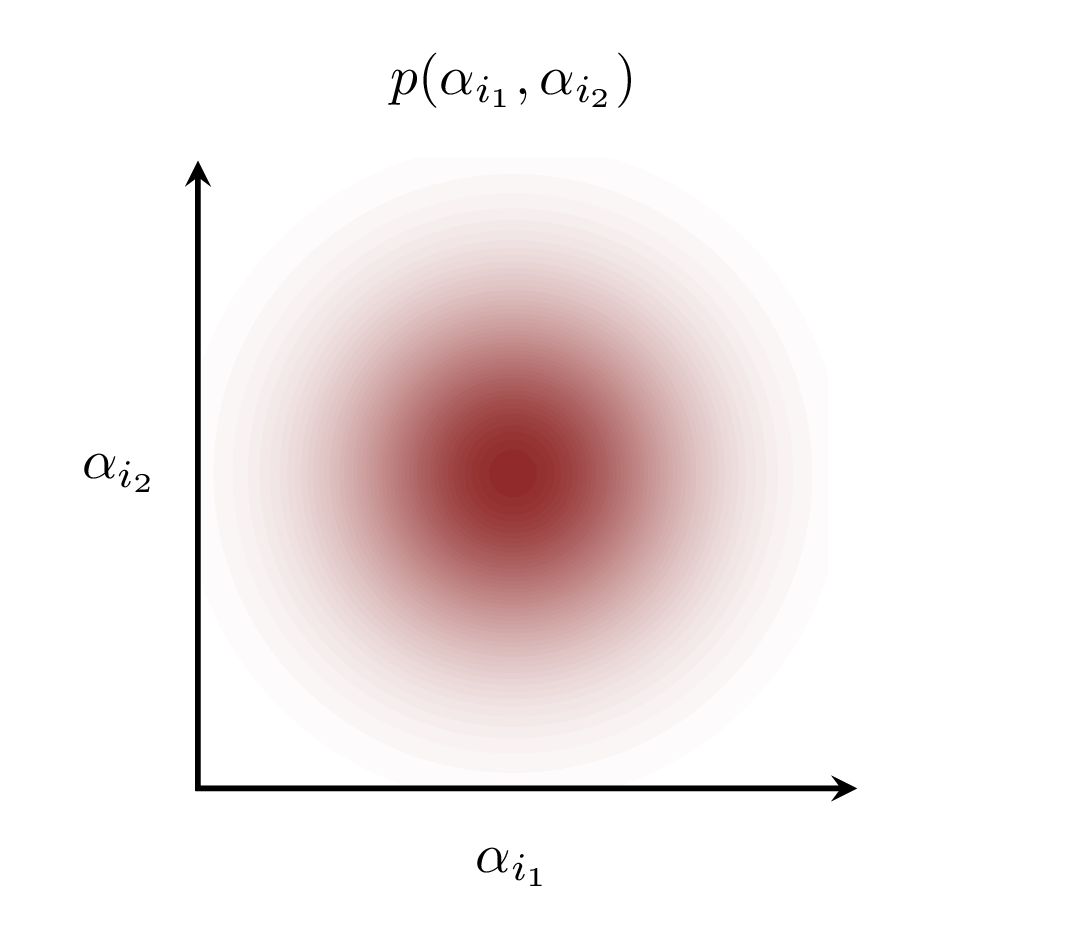
\includegraphics{figures/prior_containment/1/1.png}

}

\subcaption{\label{fig-prior-containment1}}

\end{minipage}%
%
\begin{minipage}{0.33\linewidth}

\centering{

\captionsetup{labelsep=none}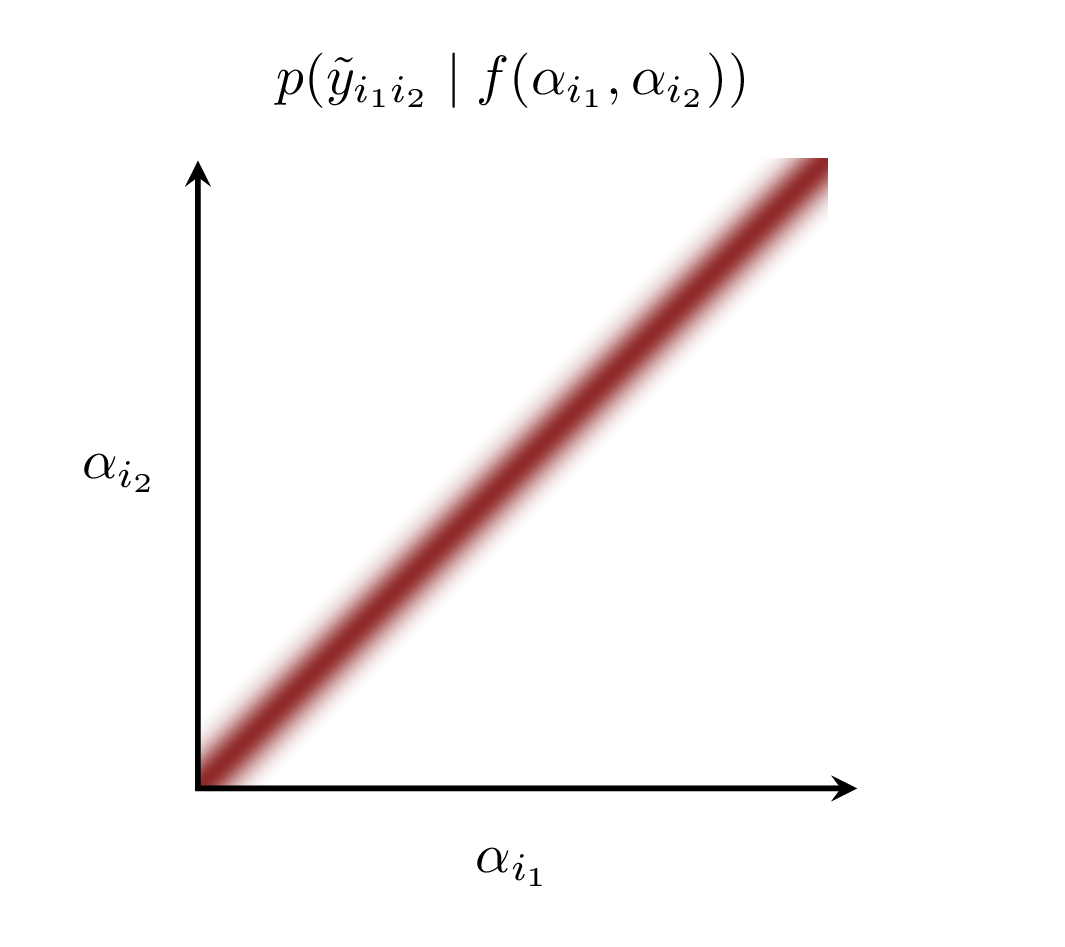
\includegraphics{figures/prior_containment/2/2.png}

}

\subcaption{\label{fig-prior-containment2}}

\end{minipage}%
%
\begin{minipage}{0.33\linewidth}

\centering{

\captionsetup{labelsep=none}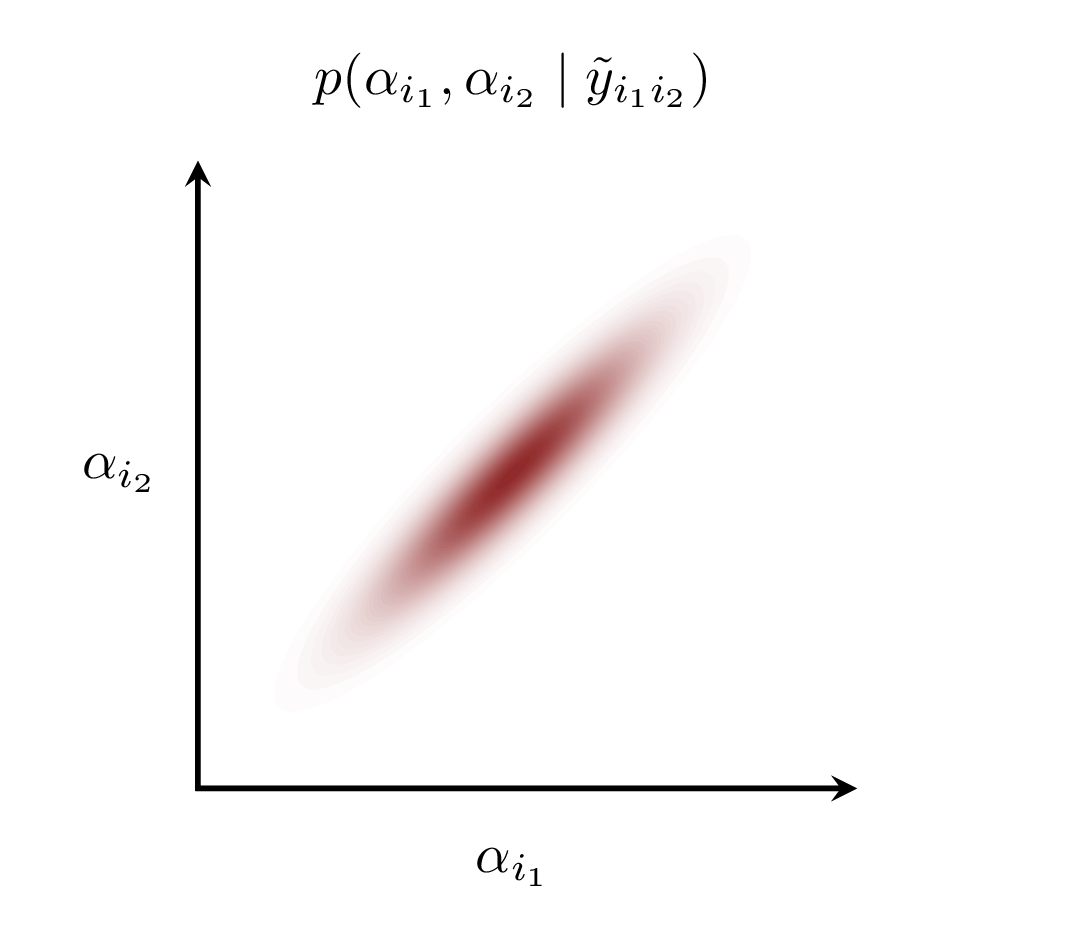
\includegraphics{figures/prior_containment/3/3.png}

}

\subcaption{\label{fig-prior-containment3}}

\end{minipage}%
%
\begin{minipage}{0.01\linewidth}
~\end{minipage}%

\caption{\label{fig-prior-containment}The item qualities in a naive
pairwise comparison model are non-identified, resulting in (b)
likelihood functions with non-compact degeneracies. (a) An informative
prior model suppresses extreme qualities, resulting in a (c) much better
behaved posterior distribution. Note, however, that a residual
degeneracy remains within the containment of the prior model.}

\end{figure}%

\subsection{Informative Prior
Modeling}\label{informative-prior-modeling}

Within a Bayesian analysis we can use an informative prior model to at
least tame these non-compact degeneracies and contain the corresponding
posterior distributions away from infinity
(Figure~\ref{fig-prior-containment}). While inferential degeneracies can
still persist within the breadth of a prior model and hinder
computational efficiency this containment at least makes accurate
computational possible.

Because we cannot interpret the item qualities independently of each
other any prior model over the \(\alpha_{i}\) will be somewhat
arbitrary. What really determines a whether a prior model is useful or
not is how consistent the \emph{induced} behavior for the differences in
item qualities, and ultimately the corresponding outcome behaviors, is
with the available domain expertise.

For example the independent component prior model over the item
qualities, \[
p( \alpha_{1}, \ldots, \alpha_{I} )
=
\prod_{i = 1}^{I} \text{normal}( \alpha_{i} \mid 0, s_{i} ),
\] implies a pushforward prior model for any item quality difference, \[
p( \alpha_{i_{1}} - \alpha_{i_{2}} )
=
\text{normal} \left( \alpha_{i_{1}} - \alpha_{i_{2}} \mid
                     0, \sqrt{ s_{i_{1}}^{2} + s_{i_{2}}^{2} } \right).
\] If this pushforward behavior is consistent with our domain expertise
then the initial prior model will be satisfactory.

That said many distinct prior models will in general share the same
pushforward behavior. In particular any independent component prior
model of the form \[
p( \alpha_{1}, \ldots, \alpha_{I} )
=
\prod_{i = 1}^{I} \text{normal}( \alpha_{i} \mid m, s_{i} )
\] implies the same pushforward behavior, \[
p( \alpha_{i_{1}} - \alpha_{i_{2}} )
=
\text{normal} \left( \alpha_{i_{1}} - \alpha_{i_{2}} \mid
                     0, \sqrt{ s_{i_{1}}^{2} + s_{i_{2}}^{2} } \right).
\] Consequently any value of \(m\) defines an equally viable prior
model.

\subsection{Anchoring Item Qualities}\label{anchoring-item-qualities}

A more effective approach than prior containment is to remove a degree
of freedom from the pairwise comparison model and eliminate the
underlying redundancy entirely.

For example consider picking an arbitrary item and then subtracting the
distinguished item quality from all of the item qualities, \[
\delta_{i} = \alpha_{i} - \alpha_{i'}.
\] After this transformation the item quality differences are unchanged,
\begin{align*}
\mu_{i_{1} i_{2}}( \delta_{i_{1}}, \delta_{i_{2}} )
&=
\mu_{i_{1} i_{2}}( \alpha_{i_{1}} - \alpha_{i'},
                   \alpha_{i_{2}} - \alpha_{i'} )
\\
&=
f \big(  (\alpha_{i_{1}} - \alpha_{i'})
       - (\alpha_{i_{2}} - \alpha_{i'}) \big)
\\
&=
f \big( \alpha_{i_{1}} - \alpha_{i_{2}} \big)
\\
&=
\mu_{i_{1} i_{2}}( \alpha_{i_{1}}, \alpha_{i_{2}} ),
\end{align*} but the distinguished item quality is now \textbf{anchored}
to zero, \[
\delta_{i'} = \alpha_{i'} - \alpha_{i'} = 0.
\] Because \(\delta_{i'}\) is now fixed we have to infer only the
\(I - 1\) remaining quality parameters.

The \(\delta_{i}\) can be interpreted as the item qualities
\emph{relative} to the quality of the anchored item, with
\(\delta_{i} > 0\) implying that the \(i\)th item is superior to the
anchored item and \(\delta_{i} < 0\) implying that the \(i\)th item is
inferior to the anchored item. This direct interpretation also
facilitates prior modeling, allowing us to reason about the relative
item qualities directly instead of having to analyze pushforward
behavior.

All of this said, a single anchor isn't always enough. Recall that once
we fix the quality of the \(i'\)th item to zero the residual quality
parameters are interpreted relative to the quality of that anchored
item. This immediately identifies the \(\delta_{i}\) for any item that
is directly compared to the \(i'\)th item. These identified parameters
in turn identify any remaining items that are directly compared to them,
and so on.

Any items which are not at least indirectly compared to the anchored
item, however, remain invariant to translations! In order to eliminate
this remaining redundancy we need to anchor the quality of at least one
more item.

We can formalize the connectivity of the comparisons, and hence how many
item qualities we need to anchor, with a little bit of graph theory
(Clark and Holton (1991)). Any set of observed pairwise comparisons
define a graph, with each item defining a node and the number of
pairwise comparisons between any two items defining a weighted,
undirected edge between the corresponding nodes
(Figure~\ref{fig-graph}).

\begin{figure}

\centering{

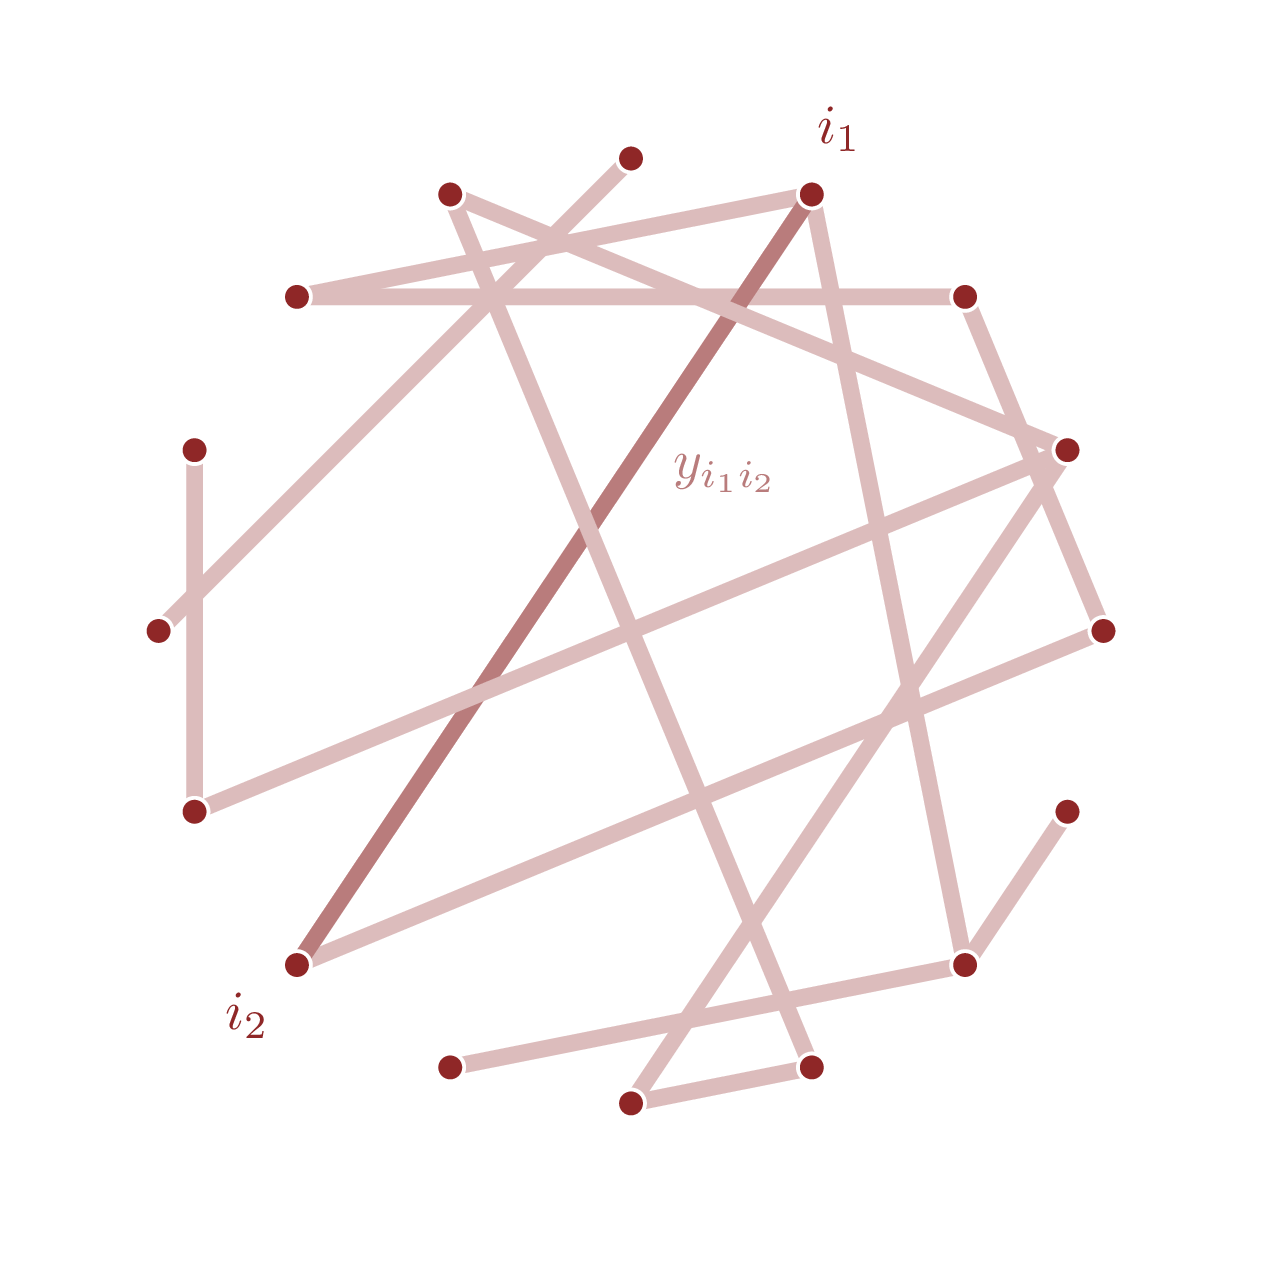
\includegraphics[width=0.5\textwidth,height=\textheight]{figures/graph/graph.png}

}

\caption{\label{fig-graph}Any collection of pairwise comparisons defines
an undirected graph, with the items being compared defining nodes and
the comparisons themselves defining edges between the nodes.}

\end{figure}%

Two items have been directly or indirectly compared inform each other if
their nodes can be connected by a path of edges. More formally these
interacting items form the connected subgraphs, or \textbf{components},
of the full graph (Figure~\ref{fig-graph-decomposition}).

\begin{figure}

\begin{minipage}{0.01\linewidth}
~\end{minipage}%
%
\begin{minipage}{0.33\linewidth}

\centering{

\captionsetup{labelsep=none}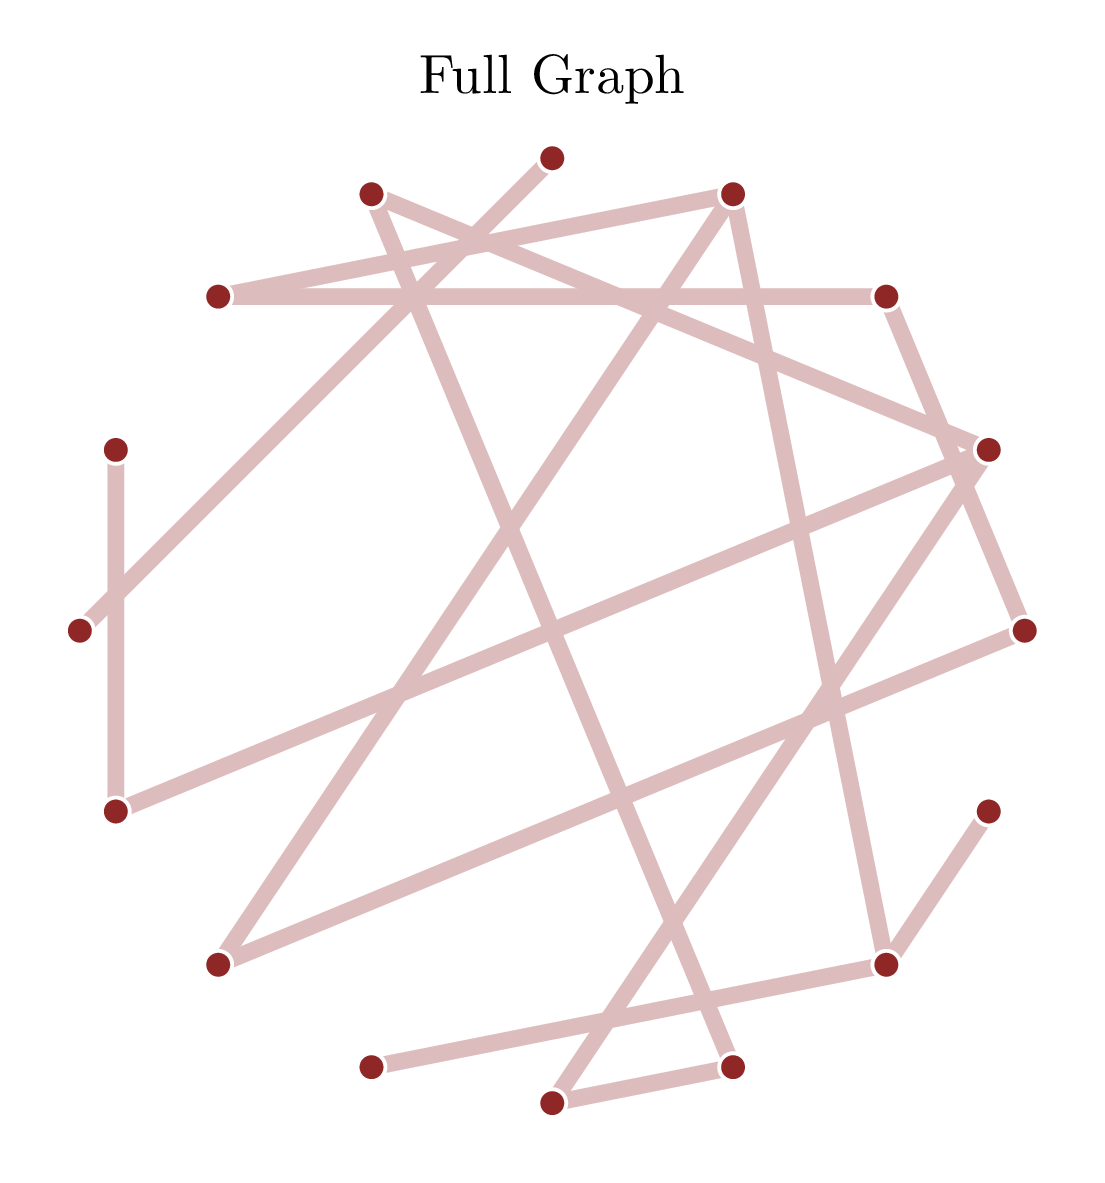
\includegraphics{figures/graph_decomposition/1/1.png}

}

\subcaption{\label{fig-graph-decomposition1}}

\end{minipage}%
%
\begin{minipage}{0.33\linewidth}

\centering{

\captionsetup{labelsep=none}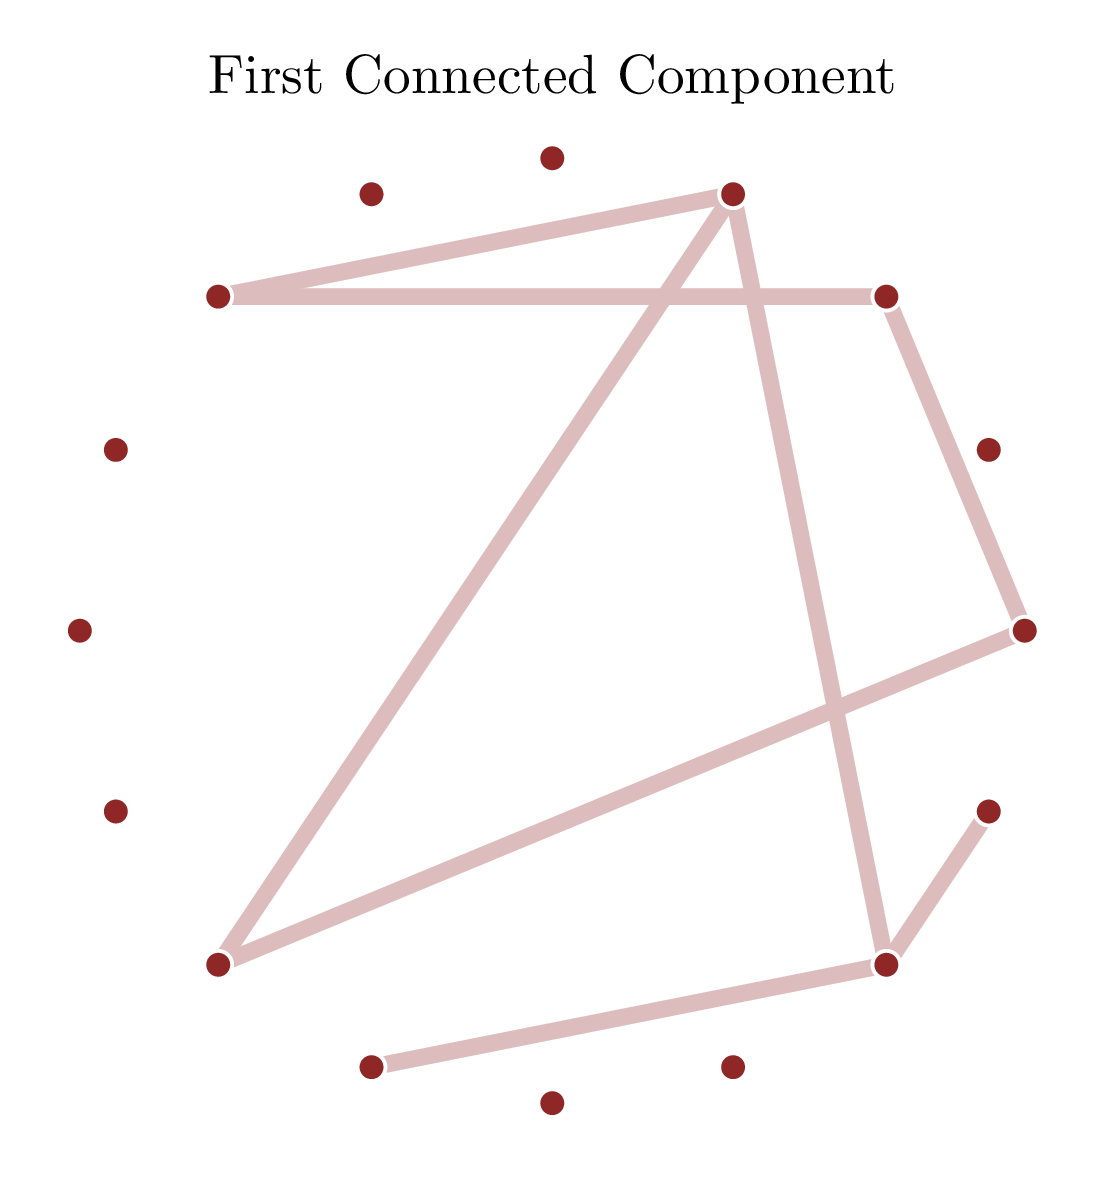
\includegraphics{figures/graph_decomposition/2/2.png}

}

\subcaption{\label{fig-graph-decomposition2}}

\end{minipage}%
%
\begin{minipage}{0.33\linewidth}

\centering{

\captionsetup{labelsep=none}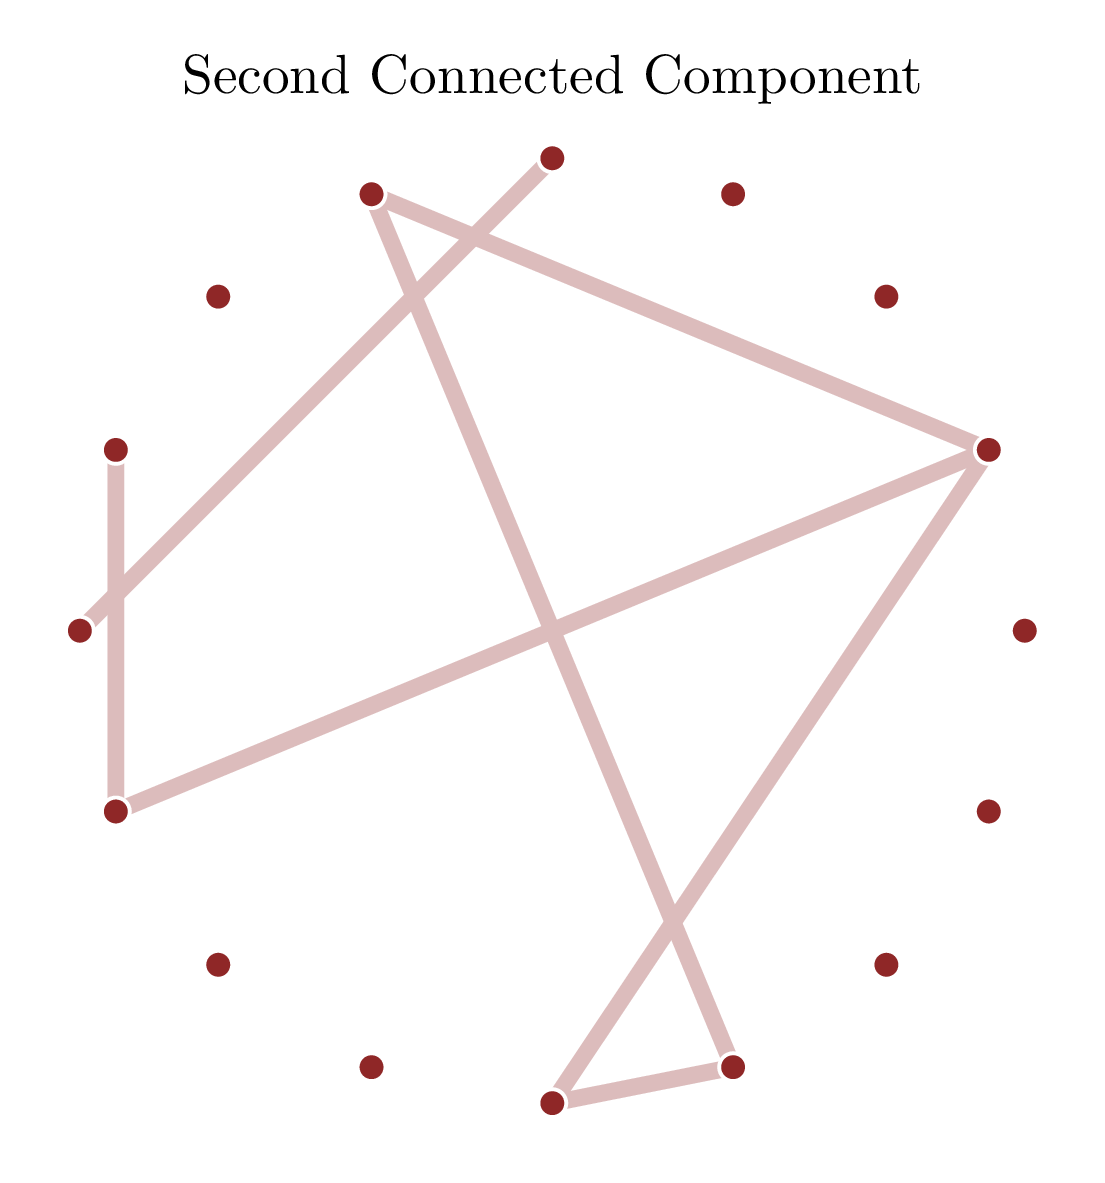
\includegraphics{figures/graph_decomposition/3/3.png}

}

\subcaption{\label{fig-graph-decomposition3}}

\end{minipage}%
%
\begin{minipage}{0.01\linewidth}
~\end{minipage}%

\caption{\label{fig-graph-decomposition}When some nodes are isolated
from the others (a) a graph decomposes into (b, c) multiple connected
components. In a graph defined by pairwise comparisons the item
qualities in any one component are independent of the item qualities in
any other component.}

\end{figure}%

From an inferential perspective the behavior of items in one connected
component are independent of the behavior of items in any other
connected component. In particular anchoring the quality parameter of an
item eliminates the redundancy only of the item qualities within the
same component. The redundancy of item qualities in other components
remains.

To completely eliminate the redundancy of a pairwise component model and
avoid the subsequent inferential degeneracies we have to anchor one item
quality \emph{in each connected component}. Fortunately the translation
of a collection of items into a graph and computation of the resulting
connected components is relatively straightforward to implement in
practice (Cormen et al. (2022)). We'll review a demonstration in
\hyperref[sec:graph-utils]{Section 6.2}.

Another consequence of these connectivity considerations is that the
item qualities are only \emph{locally} interpretable within the
encompassing connected component. We cannot relate items that have no
connection to each other! For example while we can learn the relative
test-taking abilities of students who take the same test we cannot
compare students who have taken completely different tests. Similarly
when analyzing historical competition data we can learn how skilled more
modern competitors are to older competitors only if we have enough
intermediate competitions to bridge them together.

\subsection{Coupling Function
Redundancies}\label{coupling-function-redundancies}

Every function that couples the item quality differences to the outcome
location will suffer the fundamental redundancy of the item qualities.
Some coupling functions, however, can introduce new redundancies and
inferential degeneracies with them.

Consider, for example, the translation function \[
t_{\eta} ( \alpha_{i_{1}} - \alpha_{i_{2}} )
=
\eta + \alpha_{i_{1}} - \alpha_{i_{2}}.
\] Mathematically the baseline suffers from an additive redundancy with
the item quality differences, \begin{align*}
t_{\eta} ( \alpha_{i_{1}} - \alpha_{i_{2}} )
&=
\eta + \alpha_{i_{1}} - \alpha_{i_{2}}
\\
&=
\eta + 0 + \alpha_{i_{1}} - \alpha_{i_{2}}
\\
&=
\eta + \zeta - \zeta + \alpha_{i_{1}} - \alpha_{i_{2}}
\\
&=
(\eta + \zeta) + (\alpha_{i_{1}} - \alpha_{i_{2}} - \zeta)
\\
&=
t_{\eta + \zeta} (\alpha_{i_{1}} - \alpha_{i_{2}} - \zeta ).
\end{align*}

When items appear are both side of the comparisons, however, there's no
way to factor that offset \(\zeta\) into the individual item qualities.
In this case the baseline \(\eta\) is identified by the observed
behavior common to all comparisons.

With bi-partite comparisons, however, we can factor any offset \(\zeta\)
into either of the contrasting item qualities \begin{align*}
t_{\eta} ( \alpha_{i} - \beta_{j} )
&=
t_{\eta + \zeta} ( \alpha_{i} - \beta_{j} - \zeta )
\\
&=
t_{\eta + \zeta} \big( (\alpha_{i} - \zeta) - \beta_{j} \big)
\\
&=
t_{\eta + \zeta} \big( \alpha_{i} - (\beta_{j} + \zeta) \big).
\end{align*} Because we can absorb the offset into either group of item
qualities we cannot eliminate this redundancy by anchoring one type of
item alone. Instead we have to anchor both types of items.

When the observed comparisons define a single connected component we
need to set a distinguished \(\alpha_{i'}\) and a distinguished
\(\beta_{j'}\) to zero at the same time. More generally we need to fix
one of each type of item quality within each connected component.

For example if we're modeling points scored in the games of a sports
league as \[
p(y_{ij} ) =
\mathrm{Poisson}\big( y_{ij} \mid
                      \exp(  \eta
                           + \alpha_{i}^{\mathrm{offense}}
                           - \alpha_{j}^{\mathrm{defense}}
                          )
                \big)
\] then we would need to anchor one team's offensive skill to zero and
one team's defensive skill to zero so that the remaining skills are
defined relative to the anchored skills. In general we can anchor the
offensive and defensive skills of the same team or even different teams.
Either way we can then interpret the baseline \(\eta\) as modeling the
score in a, possibly hypothetical, game between the anchored offense and
the anchored defense.

Similarly a scaling function \[
s_{\gamma} (\alpha_{i_{1}} - \alpha_{i_{2}} )
=
\gamma \cdot (\alpha_{i_{1}} - \alpha_{i_{2}}).
\] suffers from a multiplicative redundancy, \begin{align*}
s_{\gamma} (\alpha_{i_{1}} - \alpha_{i_{2}} )
&=
\gamma \cdot (\alpha_{i_{1}} - \alpha_{i_{2}})
\\
&=
\gamma \cdot 1 \cdot (\alpha_{i_{1}} - \alpha_{i_{2}})
\\
&=
\gamma \cdot \frac{\rho}{\rho} \cdot (\alpha_{i_{1}} - \alpha_{i_{2}})
\\
&=
(\rho \cdot \gamma) \cdot
\left( \frac{\alpha_{i_{1}} - \alpha_{i_{2}}}{\rho} \right)
\\
&=
s_{\rho \cdot \gamma}
\left( \frac{\alpha_{i_{1}} - \alpha_{i_{2}}}{\rho} \right).
\end{align*}

Because scaling the item qualities does not obstruct translations, \[
\frac{\alpha_{i_{1}} - \alpha_{i_{2}}}{\rho}
=
\frac{ (\alpha_{i_{1}} + \zeta) - (\alpha_{i_{2}} - \zeta)}{\rho},
\] anchoring the item qualities will not eliminate this scale
redundancy. \emph{Any} proportional increase in the discrimination
parameter \(\gamma\) can be compensated by a proportional decrease in
the item qualities and vice versa.

An informative prior model on the item qualities and discrimination
parameters does limit the scope of this redundancy, and hence the
resulting inferential degeneracies. That said constraints on the
qualities and discriminations can interact in subtle ways that
complicate principled prior modeling. By far the most effective strategy
is to eliminate the redundancy entirely.

If the discrimination is homogeneous across all comparisons then we can
always fix \(\gamma\) to one without any loss of generality. On the
other hand if the discrimination is heterogeneous, with a separate
\(\gamma_{k}\) for each distinct context, then fixing one of the
\(\gamma_{k'}\) will eliminate the redundancy in the pairwise comparison
model. Specifically if we set \[
\gamma_{k'} = 1
\] then the remaining discrimination parameters end up quantifying
scaling relative to the anchored context, \[
\kappa_{k} = \frac{ \gamma_{k} }{ \gamma_{k'} }.
\]

\subsection{Trouble With Dominating
Items}\label{trouble-with-dominating-items}

Depending on the structure of the observational space pairwise
comparison models can also suffer from some more circumstantial
inferential degeneracies.

Consider for example comparison outcomes that are bounded above, \[
y_{i_{1} i_{2}} \le y_{\max}.
\] If the observed comparisons to one particular item \(i'\) always
saturate that maximum value, \[
y_{i' i_{2}} = y_{\max},
\] then the observations will not be able to determine just how much
better that dominating item is from the others.

The saturated observations will be able to lower bound the definite or
relative quality of the dominating item, but they will be indifferent to
the remaining, arbitrarily large values. This then results in a
non-compact degeneracy extending out towards positively-infinite values.

Similarly if the observed comparisons are bounded below, \[
y_{i_{1} i_{2}} \ge y_{\min},
\] and the observed comparisons to one dominating item always saturate
that minimum value, \[
y_{i' i_{2}} = y_{\min},
\] then the data will not be able to differentiate between arbitrarily
large but negative values of the definite quality \(\alpha_{i'}\) or
even the relative quality \(\delta_{i'}\). In this case the likelihood
function will exhibit a non-compact degeneracy that extends out towards
negatively-infinite values.

For both cases a reasonably informative prior model will be able contain
these inferential degeneracies and prevent them from propagating to the
posterior distribution. An even better strategy is to design more
informative comparisons that can inform just how much better every item
is from its peers.

For example in the context of sporting events analyzing score
differentials is always more informative than analyzing winners.
Similarly in the context of standardized testing one might be able to
learn more from how long it takes students to reach the right answer
than one can from whether or not the students report the right answer
eventually.

\section{Ranking Items}\label{ranking-items}

Because item qualities can be meaningfully interpreted only relative to
one other they inform only a limited range of behaviors. One
particularly useful behavior that they can inform are \emph{rankings} of
the items being compared.

Formally any configuration of item qualities, \[
( \alpha_{1}, \ldots, \alpha_{i}, \ldots, \alpha_{I} ) \in A^{I},
\] implies one of \(I!\) possible rankings, \[
(r_{1}, \ldots, r_{i}, \ldots, r_{I}) \in R,
\] where the items are ordered by their relative qualities, \[
\alpha_{r_{1}} < \ldots <
\alpha_{r_{i}} < \ldots <
\alpha_{r_{I}}.
\] In fact this relationship defines a bijective function from the space
of item qualities to the space of the possible orderings of the \(I\)
items, \[
o : A^{I} \rightarrow R.
\]

Theoretically pushing forward a posterior distribution over the item
qualities \(\pi\) along this function will define a posterior
distribution \(o_{*} \pi\) that quantifies the consistent item rankings.
The challenge in practice, however, is that the space of ranking \(R\)
is difficult to navigate. In particular it is not immediately clear how
we might be able to construct summaries of \(o_{*} \pi\) that are
straightforward to communicate.

For example we might be interested in point summaries that quantify the
centrality of the rank posterior distribution in some way. Because the
space of rankings is discrete each rank will in general be allocated
non-zero probability, allowing us to consider a modal ranking, \[
r^{*} = \underset{r \in R}{\mathrm{argmax}} \; o_{*} \pi( \{ r \} ).
\]

Unfortunately even if a unique mode exists actually finding it is
typically intractable. In general we will not be able to compute the
atomic allocations \(o_{*} \pi( \{ r \} )\) in closed form and
estimation of all of these probabilities quickly becomes expensive.
Consequently exhaustively searching through all \(I!\) atomic
allocations is almost always be too expensive. Moreover without gradient
information we have no way to guide a more efficient search of the
ranking space.

In analogy to the construction of posterior mean summaries we might
instead consider a ranking distance function
\(d : R \times R \rightarrow \mathbb{R}^{+}\) and then define a point
summary that minimizes the expected distance, \[
\mu_{R}
=
\underset{r \in R}{\mathrm{argmin}} \;
\mathbb{E}_{o_{*} \pi}[ d( \cdot, r) ].
\] Conveniently there are a variety of useful distance functions on
\(R\) that we could use to inform such point summaries, and in theory we
can estimate the necessary expectation values with Markov chain Monte
Carlo. The minimization over all possible candidate rankings
\(r \in R\), however, suffers from the same problems as above.

Because of these computational issues we usually need to appeal to more
heuristic summaries in practice. For instance we can always rank the
items by the posterior expectation values of their individual qualities,
\[
\mathbb{E}_{\pi}[ \alpha_{r_{1}} ] < \ldots <
\mathbb{E}_{\pi}[ \alpha_{r_{i}} ] < \ldots <
\mathbb{E}_{\pi}[ \alpha_{r_{I}} ].
\]

When considering only two items at a time we can can also consult the
posterior probability that one skill surpasses the other, \[
\pi( \{ \alpha_{i_{1}} > \alpha_{i_{2}} \} ).
\] One nice feature of this pairwise inferential comparison is that it
accounts for any coupled uncertainties between the two item qualities.

These binary inferential comparisons can also be used to construct
another heuristic ranking. The posterior probability that the quality of
each item is larger than the quality of all other items, \[
p_{i'} = \pi( \{ \alpha_{i'} > \alpha_{1} \,
                 \text{and} \, \ldots \, \text{and} \,
                 \alpha_{i'} > \alpha_{i} \,
                 \text{and} \, \ldots \, \text{and} \,
                 \alpha_{i'} > \alpha_{I} \}),
\] can be used to assign a top rank, \[
r_{I} = \underset{i \in I}{\mathrm{argmax}} \; p_{i}.
\] At this point we can compute the posterior probability that the
quality of each remaining item is larger than the quality of all of the
other remaining items and assign the second-highest rank based on the
largest of these probabilities. We can then fill out all of the
remaining rankings by iterating this procedure until only one item is
left to occupy the lowest rank.

The main limitations with this approach is that it requires estimating
so many probability allocations that we can exhaust the available
computational resources, especially if there are a lot of items. The
computation is even more demanding if we want to ensure robust rankings
that are not corrupted by computational artifacts. This requires that
the Markov chain Monte Carlo error for each posterior probability
estimate is smaller than any of the differences between it and the other
posterior probability estimates. Implementing robust rankings in
practice requires not only carefully monitor the error of all of the
posterior probability estimates but also potentially running additional
or longer Markov chains to reduce any errors as needed.

\section{Demonstrations}\label{demonstrations}

With the foundations laid let's investigate the implementation of
pairwise comparison models and their inferential behaviors with a series
of increasingly more sophisticated example analyses.

\subsection{Setup}\label{setup}

First and foremost we have to set up or local \texttt{R} environment.

\begin{Shaded}
\begin{Highlighting}[]
\FunctionTok{par}\NormalTok{(}\AttributeTok{family=}\StringTok{"serif"}\NormalTok{, }\AttributeTok{las=}\DecValTok{1}\NormalTok{, }\AttributeTok{bty=}\StringTok{"l"}\NormalTok{,}
    \AttributeTok{cex.axis=}\DecValTok{1}\NormalTok{, }\AttributeTok{cex.lab=}\DecValTok{1}\NormalTok{, }\AttributeTok{cex.main=}\DecValTok{1}\NormalTok{,}
    \AttributeTok{xaxs=}\StringTok{"i"}\NormalTok{, }\AttributeTok{yaxs=}\StringTok{"i"}\NormalTok{, }\AttributeTok{mar =} \FunctionTok{c}\NormalTok{(}\DecValTok{5}\NormalTok{, }\DecValTok{5}\NormalTok{, }\DecValTok{3}\NormalTok{, }\DecValTok{5}\NormalTok{))}
\end{Highlighting}
\end{Shaded}

\begin{Shaded}
\begin{Highlighting}[]
\FunctionTok{library}\NormalTok{(rstan)}
\FunctionTok{rstan\_options}\NormalTok{(}\AttributeTok{auto\_write =} \ConstantTok{TRUE}\NormalTok{)            }\CommentTok{\# Cache compiled Stan programs}
\FunctionTok{options}\NormalTok{(}\AttributeTok{mc.cores =}\NormalTok{ parallel}\SpecialCharTok{::}\FunctionTok{detectCores}\NormalTok{()) }\CommentTok{\# Parallelize chains}
\NormalTok{parallel}\SpecialCharTok{:::}\FunctionTok{setDefaultClusterOptions}\NormalTok{(}\AttributeTok{setup\_strategy =} \StringTok{"sequential"}\NormalTok{)}

\FunctionTok{library}\NormalTok{(colormap)}
\end{Highlighting}
\end{Shaded}

\begin{Shaded}
\begin{Highlighting}[]
\NormalTok{util }\OtherTok{\textless{}{-}} \FunctionTok{new.env}\NormalTok{()}
\FunctionTok{source}\NormalTok{(}\StringTok{\textquotesingle{}mcmc\_analysis\_tools\_rstan.R\textquotesingle{}}\NormalTok{, }\AttributeTok{local=}\NormalTok{util)}
\FunctionTok{source}\NormalTok{(}\StringTok{\textquotesingle{}mcmc\_visualization\_tools.R\textquotesingle{}}\NormalTok{, }\AttributeTok{local=}\NormalTok{util)}
\end{Highlighting}
\end{Shaded}

\subsection{Graph Analysis Utilities}\label{sec:graph-utils}

Next we'll need some utilities for analyzing the graphs defined by a
collection of pairwise comparisons. There are a variety of dedicated
graph analysis packages available in \texttt{R}, but here I'll code up
basic implementations of the specific tools that we'll need.

Firstly we'll need a function that builds up a weighted
\textbf{adjacency matrix} from a list of pairwise comparisons. The
\((i_{1}, i_{2})\)-th element of a weighted adjacency matrix is the
number of comparisons between item \(i_{1}\) and item \(i_{2}\). In
particular if the \((i_{1}, i_{2})\)-th element is zero then the two
items have not been directly compared.

\begin{Shaded}
\begin{Highlighting}[]
\NormalTok{build\_adj\_matrix }\OtherTok{\textless{}{-}} \ControlFlowTok{function}\NormalTok{(N\_items, N\_comparisons, idx1, idx2) \{}
  \ControlFlowTok{if}\NormalTok{ (}\FunctionTok{min}\NormalTok{(idx1) }\SpecialCharTok{\textless{}} \DecValTok{1} \SpecialCharTok{|} \FunctionTok{max}\NormalTok{(idx1) }\SpecialCharTok{\textgreater{}}\NormalTok{ N\_items) \{}
    \FunctionTok{stop}\NormalTok{(}\StringTok{"Out of bounds idx1 values."}\NormalTok{)}
\NormalTok{  \}}
  \ControlFlowTok{if}\NormalTok{ (}\FunctionTok{min}\NormalTok{(idx2) }\SpecialCharTok{\textless{}} \DecValTok{1} \SpecialCharTok{|} \FunctionTok{max}\NormalTok{(idx2) }\SpecialCharTok{\textgreater{}}\NormalTok{ N\_items) \{}
    \FunctionTok{stop}\NormalTok{(}\StringTok{"Out of bounds idx2 values."}\NormalTok{)}
\NormalTok{  \}}

\NormalTok{  adj }\OtherTok{\textless{}{-}} \FunctionTok{matrix}\NormalTok{(}\DecValTok{0}\NormalTok{, }\AttributeTok{nrow=}\NormalTok{N\_items, }\AttributeTok{ncol=}\NormalTok{N\_items)}

  \CommentTok{\# Compute directed edges}
  \ControlFlowTok{for}\NormalTok{ (n }\ControlFlowTok{in} \DecValTok{1}\SpecialCharTok{:}\NormalTok{N\_comparisons) \{}
\NormalTok{    adj[idx1[n], idx2[n]] }\OtherTok{\textless{}{-}}\NormalTok{ adj[idx1[n], idx2[n]] }\SpecialCharTok{+} \DecValTok{1}
\NormalTok{  \}}

  \CommentTok{\# Compute symmetric, undirected edges}
  \ControlFlowTok{for}\NormalTok{ (p1 }\ControlFlowTok{in} \DecValTok{1}\SpecialCharTok{:}\NormalTok{(N\_items }\SpecialCharTok{{-}} \DecValTok{1}\NormalTok{)) \{}
    \ControlFlowTok{for}\NormalTok{ (p2 }\ControlFlowTok{in}\NormalTok{ (p1 }\SpecialCharTok{+} \DecValTok{1}\NormalTok{)}\SpecialCharTok{:}\NormalTok{N\_items) \{}
\NormalTok{      N1 }\OtherTok{\textless{}{-}}\NormalTok{ adj[p1, p2]}
\NormalTok{      N2 }\OtherTok{\textless{}{-}}\NormalTok{ adj[p2, p1]}
\NormalTok{      adj[p1, p2] }\OtherTok{\textless{}{-}}\NormalTok{ N1 }\SpecialCharTok{+}\NormalTok{ N2}
\NormalTok{      adj[p2, p1] }\OtherTok{\textless{}{-}}\NormalTok{ N1 }\SpecialCharTok{+}\NormalTok{ N2}
\NormalTok{    \}}
\NormalTok{  \}}

\NormalTok{  (adj)}
\NormalTok{\}}
\end{Highlighting}
\end{Shaded}

Adjacency matrices are extremely useful for implementing many graph
theory operations in practice. For example we can use a weighed
adjacency matrix to visualize the comparison graph, with circles
representing each node and lines representing the edges. Here the color
of the lines visualizes the weight of each edge, equivalently how many
comparisons have been made between any two items.

\begin{Shaded}
\begin{Highlighting}[]
\NormalTok{plot\_undir\_graph }\OtherTok{\textless{}{-}} \ControlFlowTok{function}\NormalTok{(adj) \{}
  \ControlFlowTok{if}\NormalTok{ (}\SpecialCharTok{!}\FunctionTok{is.matrix}\NormalTok{(adj)) \{}
    \FunctionTok{stop}\NormalTok{(}\StringTok{"Input adj is not a matrix."}\NormalTok{)}
\NormalTok{  \}}
  \ControlFlowTok{if}\NormalTok{ (}\FunctionTok{nrow}\NormalTok{(adj) }\SpecialCharTok{!=} \FunctionTok{ncol}\NormalTok{(adj)) \{}
    \FunctionTok{stop}\NormalTok{(}\StringTok{"Input adj is not a square matrix."}\NormalTok{)}
\NormalTok{  \}}

\NormalTok{  nom\_colors }\OtherTok{\textless{}{-}} \FunctionTok{c}\NormalTok{(}\StringTok{"\#DCBCBC"}\NormalTok{, }\StringTok{"\#C79999"}\NormalTok{, }\StringTok{"\#B97C7C"}\NormalTok{, }\StringTok{"\#A25050"}\NormalTok{)}
\NormalTok{  edge\_colors }\OtherTok{\textless{}{-}} \FunctionTok{colormap}\NormalTok{(}\AttributeTok{colormap=}\NormalTok{nom\_colors, }\AttributeTok{nshades=}\DecValTok{100}\NormalTok{)}

\NormalTok{  I }\OtherTok{\textless{}{-}} \FunctionTok{nrow}\NormalTok{(adj)}
\NormalTok{  delta }\OtherTok{\textless{}{-}} \DecValTok{2} \SpecialCharTok{*}\NormalTok{ pi }\SpecialCharTok{/}\NormalTok{ I}
\NormalTok{  thetas }\OtherTok{\textless{}{-}}\NormalTok{ (}\DecValTok{0}\SpecialCharTok{:}\NormalTok{(I }\SpecialCharTok{{-}} \DecValTok{1}\NormalTok{)) }\SpecialCharTok{*}\NormalTok{ delta }\SpecialCharTok{+}\NormalTok{ pi }\SpecialCharTok{/} \DecValTok{2}
\NormalTok{  R }\OtherTok{\textless{}{-}} \DecValTok{1}

\NormalTok{  xs }\OtherTok{\textless{}{-}}\NormalTok{ R }\SpecialCharTok{*} \FunctionTok{cos}\NormalTok{(thetas)}
\NormalTok{  ys }\OtherTok{\textless{}{-}}\NormalTok{ R }\SpecialCharTok{*} \FunctionTok{sin}\NormalTok{(thetas)}

  \FunctionTok{plot}\NormalTok{(}\DecValTok{0}\NormalTok{, }\AttributeTok{type=}\StringTok{\textquotesingle{}n\textquotesingle{}}\NormalTok{, }\AttributeTok{axes=}\ConstantTok{FALSE}\NormalTok{, }\AttributeTok{ann=}\ConstantTok{FALSE}\NormalTok{,}
       \AttributeTok{xlim=}\FunctionTok{c}\NormalTok{(}\SpecialCharTok{{-}}\FloatTok{1.1} \SpecialCharTok{*}\NormalTok{ R, }\SpecialCharTok{+}\FloatTok{1.1} \SpecialCharTok{*}\NormalTok{ R), }\AttributeTok{ylim=}\FunctionTok{c}\NormalTok{(}\SpecialCharTok{{-}}\FloatTok{1.1} \SpecialCharTok{*}\NormalTok{ R, }\SpecialCharTok{+}\FloatTok{1.1} \SpecialCharTok{*}\NormalTok{ R))}

\NormalTok{  cthetas }\OtherTok{\textless{}{-}} \FunctionTok{seq}\NormalTok{(}\DecValTok{0}\NormalTok{, }\DecValTok{2} \SpecialCharTok{*}\NormalTok{ pi }\SpecialCharTok{+} \FloatTok{0.05}\NormalTok{, }\FloatTok{0.05}\NormalTok{)}
\NormalTok{  cxs }\OtherTok{\textless{}{-}}\NormalTok{ R }\SpecialCharTok{*} \FunctionTok{cos}\NormalTok{(cthetas)}
\NormalTok{  cys }\OtherTok{\textless{}{-}}\NormalTok{ R }\SpecialCharTok{*} \FunctionTok{sin}\NormalTok{(cthetas)}
  \FunctionTok{lines}\NormalTok{(cxs, cys, }\AttributeTok{lwd=}\DecValTok{3}\NormalTok{, }\AttributeTok{col=}\StringTok{"\#DDDDDD"}\NormalTok{)}

\NormalTok{  max\_adj }\OtherTok{\textless{}{-}} \FunctionTok{max}\NormalTok{(adj)}
  \ControlFlowTok{for}\NormalTok{ (i1 }\ControlFlowTok{in} \DecValTok{1}\SpecialCharTok{:}\NormalTok{(I }\SpecialCharTok{{-}} \DecValTok{1}\NormalTok{)) \{}
    \ControlFlowTok{for}\NormalTok{ (i2 }\ControlFlowTok{in}\NormalTok{ (i1 }\SpecialCharTok{+} \DecValTok{1}\NormalTok{)}\SpecialCharTok{:}\NormalTok{I) \{}
\NormalTok{      cidx }\OtherTok{\textless{}{-}} \FunctionTok{floor}\NormalTok{(}\DecValTok{100} \SpecialCharTok{*}\NormalTok{ (adj[i1, i2] }\SpecialCharTok{/}\NormalTok{ max\_adj))}
      \FunctionTok{lines}\NormalTok{(xs[}\FunctionTok{c}\NormalTok{(i1, i2)], ys[}\FunctionTok{c}\NormalTok{(i1, i2)], }\AttributeTok{lwd=}\DecValTok{3}\NormalTok{, }\AttributeTok{col=}\NormalTok{edge\_colors[cidx])}
\NormalTok{    \}}
\NormalTok{  \}}

  \FunctionTok{points}\NormalTok{(xs, ys, }\AttributeTok{pch=}\DecValTok{16}\NormalTok{, }\AttributeTok{cex=}\FloatTok{1.75}\NormalTok{, }\AttributeTok{col=}\StringTok{"white"}\NormalTok{)}
  \FunctionTok{points}\NormalTok{(xs, ys, }\AttributeTok{pch=}\DecValTok{16}\NormalTok{, }\AttributeTok{cex=}\FloatTok{1.25}\NormalTok{, }\AttributeTok{col=}\NormalTok{util}\SpecialCharTok{$}\NormalTok{c\_dark)}
\NormalTok{\}}
\end{Highlighting}
\end{Shaded}

We can also use an adjacency graph to decompose an initial graph into
connected components.

Given an initial node we first find all of the nodes that are at least
indirectly related by pairwise comparisons with a recursive,
breadth-first search.

\begin{Shaded}
\begin{Highlighting}[]
\NormalTok{breadth\_first\_search }\OtherTok{\textless{}{-}} \ControlFlowTok{function}\NormalTok{(n, adj, }\AttributeTok{local\_nodes=}\FunctionTok{c}\NormalTok{()) \{}
\NormalTok{  local\_nodes }\OtherTok{\textless{}{-}} \FunctionTok{c}\NormalTok{(local\_nodes, n)}
\NormalTok{  neighbors }\OtherTok{\textless{}{-}} \FunctionTok{which}\NormalTok{(adj[n,] }\SpecialCharTok{\textgreater{}} \DecValTok{0}\NormalTok{)}
  \ControlFlowTok{for}\NormalTok{ (nn }\ControlFlowTok{in}\NormalTok{ neighbors) \{}
    \ControlFlowTok{if}\NormalTok{ (}\SpecialCharTok{!}\NormalTok{(nn }\SpecialCharTok{\%in\%}\NormalTok{ local\_nodes))}
\NormalTok{      local\_nodes }\OtherTok{\textless{}{-}} \FunctionTok{union}\NormalTok{(local\_nodes,}
                           \FunctionTok{Recall}\NormalTok{(nn, adj, local\_nodes))}
\NormalTok{  \}}
\NormalTok{  (local\_nodes)}
\NormalTok{\}}
\end{Highlighting}
\end{Shaded}

Repeating this search until we've exhausted all of the nodes identifies
the connected components.

\begin{Shaded}
\begin{Highlighting}[]
\NormalTok{compute\_connected\_components }\OtherTok{\textless{}{-}} \ControlFlowTok{function}\NormalTok{(adj) \{}
  \ControlFlowTok{if}\NormalTok{ (}\SpecialCharTok{!}\FunctionTok{is.matrix}\NormalTok{(adj)) \{}
    \FunctionTok{stop}\NormalTok{(}\StringTok{"Input adj is not a matrix."}\NormalTok{)}
\NormalTok{  \}}
  \ControlFlowTok{if}\NormalTok{ (}\FunctionTok{nrow}\NormalTok{(adj) }\SpecialCharTok{!=} \FunctionTok{ncol}\NormalTok{(adj)) \{}
    \FunctionTok{stop}\NormalTok{(}\StringTok{"Input adj is not a square matrix."}\NormalTok{)}
\NormalTok{  \}}

\NormalTok{  all\_nodes }\OtherTok{\textless{}{-}} \DecValTok{1}\SpecialCharTok{:}\FunctionTok{nrow}\NormalTok{(adj)}
\NormalTok{  remaining\_nodes }\OtherTok{\textless{}{-}}\NormalTok{ all\_nodes}
\NormalTok{  components }\OtherTok{\textless{}{-}} \FunctionTok{list}\NormalTok{()}

  \ControlFlowTok{for}\NormalTok{ (n }\ControlFlowTok{in}\NormalTok{ all\_nodes) \{}
    \ControlFlowTok{if}\NormalTok{ (n }\SpecialCharTok{\%in\%}\NormalTok{ remaining\_nodes) \{}
\NormalTok{      subgraph }\OtherTok{\textless{}{-}} \FunctionTok{breadth\_first\_search}\NormalTok{(n, adj)}
\NormalTok{      remaining\_nodes }\OtherTok{\textless{}{-}} \FunctionTok{setdiff}\NormalTok{(remaining\_nodes, subgraph)}
\NormalTok{      components[[}\FunctionTok{length}\NormalTok{(components) }\SpecialCharTok{+} \DecValTok{1}\NormalTok{]] }\OtherTok{\textless{}{-}}\NormalTok{ subgraph}
\NormalTok{    \}}
\NormalTok{  \}}

\NormalTok{  (components)}
\NormalTok{\}}
\end{Highlighting}
\end{Shaded}

For example let's say that we have a graph defined by \(8\) items and
\(8\) comparisons.

\begin{Shaded}
\begin{Highlighting}[]
\NormalTok{K }\OtherTok{\textless{}{-}} \DecValTok{8}
\NormalTok{C }\OtherTok{\textless{}{-}} \DecValTok{8}

\NormalTok{item1 }\OtherTok{\textless{}{-}} \FunctionTok{c}\NormalTok{(}\DecValTok{1}\NormalTok{, }\DecValTok{2}\NormalTok{, }\DecValTok{3}\NormalTok{, }\DecValTok{4}\NormalTok{, }\DecValTok{4}\NormalTok{, }\DecValTok{4}\NormalTok{, }\DecValTok{5}\NormalTok{, }\DecValTok{7}\NormalTok{)}
\NormalTok{item2 }\OtherTok{\textless{}{-}} \FunctionTok{c}\NormalTok{(}\DecValTok{2}\NormalTok{, }\DecValTok{3}\NormalTok{, }\DecValTok{1}\NormalTok{, }\DecValTok{5}\NormalTok{, }\DecValTok{6}\NormalTok{, }\DecValTok{8}\NormalTok{, }\DecValTok{6}\NormalTok{, }\DecValTok{8}\NormalTok{)}
\end{Highlighting}
\end{Shaded}

These comparisons define a weighted adjacency matrix.

\begin{Shaded}
\begin{Highlighting}[]
\NormalTok{adj }\OtherTok{\textless{}{-}} \FunctionTok{build\_adj\_matrix}\NormalTok{(K, C, item1, item2)}
\end{Highlighting}
\end{Shaded}

The weighted adjacency matrix then informs a visualization of the graph.

\begin{Shaded}
\begin{Highlighting}[]
\FunctionTok{par}\NormalTok{(}\AttributeTok{mfrow=}\FunctionTok{c}\NormalTok{(}\DecValTok{1}\NormalTok{, }\DecValTok{1}\NormalTok{), }\AttributeTok{mar=}\FunctionTok{c}\NormalTok{(}\DecValTok{0}\NormalTok{, }\DecValTok{0}\NormalTok{, }\DecValTok{0}\NormalTok{, }\DecValTok{0}\NormalTok{))}

\FunctionTok{plot\_undir\_graph}\NormalTok{(adj)}
\end{Highlighting}
\end{Shaded}

\includegraphics{pairwise_comparison_modeling_files/figure-pdf/unnamed-chunk-11-1.pdf}

In this case the graph decomposes into two components.

\begin{Shaded}
\begin{Highlighting}[]
\NormalTok{components }\OtherTok{\textless{}{-}} \FunctionTok{compute\_connected\_components}\NormalTok{(adj)}
\NormalTok{components}
\end{Highlighting}
\end{Shaded}

\begin{verbatim}
[[1]]
[1] 1 2 3

[[2]]
[1] 4 5 6 8 7
\end{verbatim}

One way to visualize this decomposition is to visualize each connected
component individually.

\begin{Shaded}
\begin{Highlighting}[]
\FunctionTok{par}\NormalTok{(}\AttributeTok{mfrow=}\FunctionTok{c}\NormalTok{(}\DecValTok{1}\NormalTok{, }\DecValTok{2}\NormalTok{), }\AttributeTok{mar=}\FunctionTok{c}\NormalTok{(}\DecValTok{0}\NormalTok{, }\DecValTok{0}\NormalTok{, }\DecValTok{2}\NormalTok{, }\DecValTok{0}\NormalTok{))}
\ControlFlowTok{for}\NormalTok{ (c }\ControlFlowTok{in} \FunctionTok{seq\_along}\NormalTok{(components)) \{}
\NormalTok{  component\_adj }\OtherTok{\textless{}{-}}\NormalTok{ adj}
  \ControlFlowTok{for}\NormalTok{ (k }\ControlFlowTok{in} \DecValTok{1}\SpecialCharTok{:}\NormalTok{K) \{}
    \ControlFlowTok{if}\NormalTok{ (}\SpecialCharTok{!}\NormalTok{(k }\SpecialCharTok{\%in\%}\NormalTok{ components[[c]]))}
\NormalTok{      component\_adj[k,] }\OtherTok{\textless{}{-}} \FunctionTok{rep}\NormalTok{(}\DecValTok{0}\NormalTok{, K)}
\NormalTok{  \}}
  \FunctionTok{plot\_undir\_graph}\NormalTok{(component\_adj)}
  \FunctionTok{title}\NormalTok{(}\FunctionTok{paste}\NormalTok{(}\StringTok{"Component"}\NormalTok{, c))}
\NormalTok{\}}
\end{Highlighting}
\end{Shaded}

\includegraphics{pairwise_comparison_modeling_files/figure-pdf/unnamed-chunk-13-1.pdf}

\subsection{Modeling Binary
Comparisons}\label{modeling-binary-comparisons}

With toolbox prepared let's move onto our first example. Here we'll
emphasize inferential degeneracies with a model of binary comparisons.
To provide some basic context let's say that these binary comparisons
are the outcomes of games between two players and we're interesting in
inferring the relative skills of each player.

\subsubsection{Simulate data}\label{simulate-data}

To start we'll need to some data to analyze, including which players are
matched up in each game and the eventual winner. For this example we'll
simulate the games in two steps, using \texttt{player1\_probs} to sample
the first player and \texttt{pair\_probs} to conditionally sample their
opponent. Note the zeroes in \texttt{pair\_probs} prevent some player
matchups from occurring at all.

\begin{Shaded}
\begin{Highlighting}[]
\NormalTok{N\_players }\OtherTok{\textless{}{-}} \DecValTok{7}
\NormalTok{N\_games }\OtherTok{\textless{}{-}} \DecValTok{4000}

\NormalTok{player1\_probs }\OtherTok{\textless{}{-}} \FunctionTok{c}\NormalTok{(}\FloatTok{0.2}\NormalTok{, }\FloatTok{0.16}\NormalTok{, }\FloatTok{0.19}\NormalTok{, }\FloatTok{0.11}\NormalTok{, }\FloatTok{0.12}\NormalTok{, }\FloatTok{0.13}\NormalTok{, }\FloatTok{0.09}\NormalTok{)}

\NormalTok{pair\_probs }\OtherTok{\textless{}{-}} \FunctionTok{c}\NormalTok{(}\FloatTok{0.0}\NormalTok{, }\FloatTok{0.4}\NormalTok{, }\FloatTok{0.0}\NormalTok{, }\FloatTok{0.0}\NormalTok{, }\FloatTok{0.5}\NormalTok{, }\FloatTok{0.0}\NormalTok{, }\FloatTok{0.0}\NormalTok{,}
                \FloatTok{0.5}\NormalTok{, }\FloatTok{0.0}\NormalTok{, }\FloatTok{0.0}\NormalTok{, }\FloatTok{0.0}\NormalTok{, }\FloatTok{0.2}\NormalTok{, }\FloatTok{0.6}\NormalTok{, }\FloatTok{0.0}\NormalTok{,}
                \FloatTok{0.0}\NormalTok{, }\FloatTok{0.0}\NormalTok{, }\FloatTok{0.0}\NormalTok{, }\FloatTok{0.6}\NormalTok{, }\FloatTok{0.0}\NormalTok{, }\FloatTok{0.0}\NormalTok{, }\FloatTok{0.5}\NormalTok{,}
                \FloatTok{0.0}\NormalTok{, }\FloatTok{0.0}\NormalTok{, }\FloatTok{0.7}\NormalTok{, }\FloatTok{0.0}\NormalTok{, }\FloatTok{0.0}\NormalTok{, }\FloatTok{0.0}\NormalTok{, }\FloatTok{0.5}\NormalTok{,}
                \FloatTok{0.5}\NormalTok{, }\FloatTok{0.3}\NormalTok{, }\FloatTok{0.0}\NormalTok{, }\FloatTok{0.0}\NormalTok{, }\FloatTok{0.0}\NormalTok{, }\FloatTok{0.4}\NormalTok{, }\FloatTok{0.0}\NormalTok{,}
                \FloatTok{0.0}\NormalTok{, }\FloatTok{0.3}\NormalTok{, }\FloatTok{0.0}\NormalTok{, }\FloatTok{0.0}\NormalTok{, }\FloatTok{0.3}\NormalTok{, }\FloatTok{0.0}\NormalTok{, }\FloatTok{0.0}\NormalTok{,}
                \FloatTok{0.0}\NormalTok{, }\FloatTok{0.0}\NormalTok{, }\FloatTok{0.3}\NormalTok{, }\FloatTok{0.4}\NormalTok{, }\FloatTok{0.0}\NormalTok{, }\FloatTok{0.0}\NormalTok{, }\FloatTok{0.0}\NormalTok{)}
\NormalTok{pair\_probs }\OtherTok{\textless{}{-}}  \FunctionTok{matrix}\NormalTok{(pair\_probs, }\AttributeTok{nrow=}\NormalTok{N\_players)}
\end{Highlighting}
\end{Shaded}

\begin{codelisting}

\caption{\texttt{simu\textbackslash\_bradley\textbackslash\_terry.stan}}

\begin{Shaded}
\begin{Highlighting}[]
\KeywordTok{data}\NormalTok{ \{}
  \DataTypeTok{int}\NormalTok{\textless{}}\KeywordTok{lower}\NormalTok{=}\DecValTok{1}\NormalTok{\textgreater{} N\_players; }\CommentTok{// Number of players}
  \DataTypeTok{int}\NormalTok{\textless{}}\KeywordTok{lower}\NormalTok{=}\DecValTok{1}\NormalTok{\textgreater{} N\_games;   }\CommentTok{// Number of games}

  \CommentTok{// Matchup probabilities}
  \DataTypeTok{simplex}\NormalTok{[N\_players] player1\_probs;}
  \DataTypeTok{array}\NormalTok{[N\_players] }\DataTypeTok{simplex}\NormalTok{[N\_players] pair\_probs;}
\NormalTok{\}}

\KeywordTok{generated quantities}\NormalTok{ \{}
  \CommentTok{// Player skills}
  \DataTypeTok{array}\NormalTok{[N\_players] }\DataTypeTok{real}\NormalTok{ alpha}
\NormalTok{    = normal\_rng(rep\_vector(}\DecValTok{0}\NormalTok{, N\_players), log(sqrt(}\DecValTok{2}\NormalTok{)) / }\FloatTok{2.32}\NormalTok{);}

  \CommentTok{// Game outcomes}
  \DataTypeTok{array}\NormalTok{[N\_games] }\DataTypeTok{int}\NormalTok{\textless{}}\KeywordTok{lower}\NormalTok{=}\DecValTok{1}\NormalTok{, }\KeywordTok{upper}\NormalTok{=N\_players\textgreater{} player1\_idx;}
  \DataTypeTok{array}\NormalTok{[N\_games] }\DataTypeTok{int}\NormalTok{\textless{}}\KeywordTok{lower}\NormalTok{=}\DecValTok{1}\NormalTok{, }\KeywordTok{upper}\NormalTok{=N\_players\textgreater{} player2\_idx;}
  \DataTypeTok{array}\NormalTok{[N\_games] }\DataTypeTok{int}\NormalTok{\textless{}}\KeywordTok{lower}\NormalTok{=}\DecValTok{0}\NormalTok{, }\KeywordTok{upper}\NormalTok{=}\DecValTok{1}\NormalTok{\textgreater{} y;}

  \ControlFlowTok{for}\NormalTok{ (n }\ControlFlowTok{in} \DecValTok{1}\NormalTok{:N\_games) \{}
    \CommentTok{// Simulate first player}
\NormalTok{    player1\_idx[n] = categorical\_rng(player1\_probs);}

    \CommentTok{// Simulate second player}
\NormalTok{    player2\_idx[n] = categorical\_rng(pair\_probs[player1\_idx[n]]);}

    \CommentTok{// Simulate winner}
\NormalTok{    y[n] = bernoulli\_logit\_rng(  alpha[player1\_idx[n]]}
\NormalTok{                               {-} alpha[player2\_idx[n]]);}
\NormalTok{  \}}
\NormalTok{\}}
\end{Highlighting}
\end{Shaded}

\end{codelisting}

\begin{Shaded}
\begin{Highlighting}[]
\NormalTok{simu }\OtherTok{\textless{}{-}} \FunctionTok{stan}\NormalTok{(}\AttributeTok{file=}\StringTok{"stan\_programs/simu\_bradley\_terry.stan"}\NormalTok{,}
             \AttributeTok{algorithm=}\StringTok{"Fixed\_param"}\NormalTok{, }\AttributeTok{seed=}\DecValTok{8438338}\NormalTok{,}
             \AttributeTok{data=}\FunctionTok{list}\NormalTok{(}\StringTok{"N\_players"} \OtherTok{=}\NormalTok{ N\_players,}
                       \StringTok{"N\_games"} \OtherTok{=}\NormalTok{ N\_games,}
                       \StringTok{"player1\_probs"} \OtherTok{=}\NormalTok{ player1\_probs,}
                       \StringTok{"pair\_probs"} \OtherTok{=}\NormalTok{ pair\_probs),}
             \AttributeTok{warmup=}\DecValTok{0}\NormalTok{, }\AttributeTok{iter=}\DecValTok{1}\NormalTok{, }\AttributeTok{chains=}\DecValTok{1}\NormalTok{, }\AttributeTok{refresh=}\DecValTok{0}\NormalTok{)}
\end{Highlighting}
\end{Shaded}

\begin{Shaded}
\begin{Highlighting}[]
\NormalTok{data }\OtherTok{\textless{}{-}} \FunctionTok{list}\NormalTok{(}\StringTok{"N\_players"} \OtherTok{=}\NormalTok{ N\_players,}
             \StringTok{"N\_games"} \OtherTok{=}\NormalTok{ N\_games,}
             \StringTok{"player1\_idx"} \OtherTok{=} \FunctionTok{extract}\NormalTok{(simu)}\SpecialCharTok{$}\NormalTok{player1\_idx[}\DecValTok{1}\NormalTok{,],}
             \StringTok{"player2\_idx"} \OtherTok{=} \FunctionTok{extract}\NormalTok{(simu)}\SpecialCharTok{$}\NormalTok{player2\_idx[}\DecValTok{1}\NormalTok{,],}
             \StringTok{"y"} \OtherTok{=} \FunctionTok{extract}\NormalTok{(simu)}\SpecialCharTok{$}\NormalTok{y[}\DecValTok{1}\NormalTok{,])}

\NormalTok{alpha\_true }\OtherTok{\textless{}{-}} \FunctionTok{extract}\NormalTok{(simu)}\SpecialCharTok{$}\NormalTok{alpha[}\DecValTok{1}\NormalTok{,]}
\end{Highlighting}
\end{Shaded}

\subsubsection{Explore Data}\label{explore-data}

Now we can explore the simulated data.

Counting the number of games that include each player we can see that
not every player participates in the same number of games. Consequently
we should be able to more precisely learn the relative skills of the
more active players.

\begin{Shaded}
\begin{Highlighting}[]
\NormalTok{game\_counts }\OtherTok{\textless{}{-}} \FunctionTok{sapply}\NormalTok{(}\DecValTok{1}\SpecialCharTok{:}\NormalTok{data}\SpecialCharTok{$}\NormalTok{N\_players,}
                      \ControlFlowTok{function}\NormalTok{(i) }\FunctionTok{sum}\NormalTok{(data}\SpecialCharTok{$}\NormalTok{player1\_idx }\SpecialCharTok{==}\NormalTok{ i }\SpecialCharTok{|}
\NormalTok{                                      data}\SpecialCharTok{$}\NormalTok{player2\_idx }\SpecialCharTok{==}\NormalTok{ i   ) )}

\FunctionTok{par}\NormalTok{(}\AttributeTok{mfrow=}\FunctionTok{c}\NormalTok{(}\DecValTok{1}\NormalTok{, }\DecValTok{1}\NormalTok{), }\AttributeTok{mar=}\FunctionTok{c}\NormalTok{(}\DecValTok{5}\NormalTok{, }\DecValTok{5}\NormalTok{, }\DecValTok{1}\NormalTok{, }\DecValTok{1}\NormalTok{))}

\FunctionTok{barplot}\NormalTok{(game\_counts,}
        \AttributeTok{space=}\DecValTok{0}\NormalTok{, }\AttributeTok{col=}\NormalTok{util}\SpecialCharTok{$}\NormalTok{c\_dark\_teal, }\AttributeTok{border=}\StringTok{"white"}\NormalTok{,}
        \AttributeTok{xlab=}\StringTok{"Player"}\NormalTok{, }\AttributeTok{ylab=}\StringTok{"Number of Games"}\NormalTok{)}
\end{Highlighting}
\end{Shaded}

\includegraphics{pairwise_comparison_modeling_files/figure-pdf/unnamed-chunk-17-1.pdf}

To investigate the interaction between the players we can visualize the
matchups as a graph.

\begin{Shaded}
\begin{Highlighting}[]
\NormalTok{adj }\OtherTok{\textless{}{-}} \FunctionTok{build\_adj\_matrix}\NormalTok{(data}\SpecialCharTok{$}\NormalTok{N\_players, data}\SpecialCharTok{$}\NormalTok{N\_games,}
\NormalTok{                        data}\SpecialCharTok{$}\NormalTok{player1\_idx, data}\SpecialCharTok{$}\NormalTok{player2\_idx)}

\FunctionTok{par}\NormalTok{(}\AttributeTok{mfrow=}\FunctionTok{c}\NormalTok{(}\DecValTok{1}\NormalTok{, }\DecValTok{1}\NormalTok{), }\AttributeTok{mar=}\FunctionTok{c}\NormalTok{(}\DecValTok{0}\NormalTok{, }\DecValTok{0}\NormalTok{, }\DecValTok{0}\NormalTok{, }\DecValTok{0}\NormalTok{))}

\FunctionTok{plot\_undir\_graph}\NormalTok{(adj)}
\end{Highlighting}
\end{Shaded}

\includegraphics{pairwise_comparison_modeling_files/figure-pdf/unnamed-chunk-18-1.pdf}

Interestingly the players decompose into two isolated groups, with no
games matching up players across the groups.

\begin{Shaded}
\begin{Highlighting}[]
\NormalTok{components }\OtherTok{\textless{}{-}} \FunctionTok{compute\_connected\_components}\NormalTok{(adj)}
\NormalTok{components}
\end{Highlighting}
\end{Shaded}

\begin{verbatim}
[[1]]
[1] 1 2 5 6

[[2]]
[1] 3 4 7
\end{verbatim}

\begin{Shaded}
\begin{Highlighting}[]
\FunctionTok{par}\NormalTok{(}\AttributeTok{mfrow=}\FunctionTok{c}\NormalTok{(}\DecValTok{1}\NormalTok{, }\DecValTok{2}\NormalTok{), }\AttributeTok{mar=}\FunctionTok{c}\NormalTok{(}\DecValTok{0}\NormalTok{, }\DecValTok{0}\NormalTok{, }\DecValTok{2}\NormalTok{, }\DecValTok{0}\NormalTok{))}

\ControlFlowTok{for}\NormalTok{ (c }\ControlFlowTok{in} \FunctionTok{seq\_along}\NormalTok{(components)) \{}
\NormalTok{  component\_adj }\OtherTok{\textless{}{-}}\NormalTok{ adj}
  \ControlFlowTok{for}\NormalTok{ (i }\ControlFlowTok{in} \DecValTok{1}\SpecialCharTok{:}\NormalTok{data}\SpecialCharTok{$}\NormalTok{N\_players) \{}
    \ControlFlowTok{if}\NormalTok{ (}\SpecialCharTok{!}\NormalTok{(i }\SpecialCharTok{\%in\%}\NormalTok{ components[[c]]))}
\NormalTok{      component\_adj[i,] }\OtherTok{\textless{}{-}} \FunctionTok{rep}\NormalTok{(}\DecValTok{0}\NormalTok{, data}\SpecialCharTok{$}\NormalTok{N\_players)}
\NormalTok{  \}}
  \FunctionTok{plot\_undir\_graph}\NormalTok{(component\_adj)}
  \FunctionTok{title}\NormalTok{(}\FunctionTok{paste}\NormalTok{(}\StringTok{"Connected Subgraph"}\NormalTok{, c))}
\NormalTok{\}}
\end{Highlighting}
\end{Shaded}

\includegraphics{pairwise_comparison_modeling_files/figure-pdf/unnamed-chunk-19-1.pdf}

Given the variation in the number of games played it's no surprise that
there is also heterogeneity in the total number of wins and losses for
each player.

\begin{Shaded}
\begin{Highlighting}[]
\NormalTok{win\_counts }\OtherTok{\textless{}{-}} \FunctionTok{sapply}\NormalTok{(}\DecValTok{1}\SpecialCharTok{:}\NormalTok{data}\SpecialCharTok{$}\NormalTok{N\_players,}
                     \ControlFlowTok{function}\NormalTok{(i) }\FunctionTok{sum}\NormalTok{(( data}\SpecialCharTok{$}\NormalTok{player1\_idx }\SpecialCharTok{==}\NormalTok{ i }\SpecialCharTok{\&}
\NormalTok{                                       data}\SpecialCharTok{$}\NormalTok{y }\SpecialCharTok{==} \DecValTok{1}\NormalTok{              ) }\SpecialCharTok{|}
\NormalTok{                                     ( data}\SpecialCharTok{$}\NormalTok{player2\_idx }\SpecialCharTok{==}\NormalTok{ i }\SpecialCharTok{\&}
\NormalTok{                                       data}\SpecialCharTok{$}\NormalTok{y }\SpecialCharTok{==} \DecValTok{0}\NormalTok{              )  ) )}

\NormalTok{loss\_counts }\OtherTok{\textless{}{-}} \FunctionTok{sapply}\NormalTok{(}\DecValTok{1}\SpecialCharTok{:}\NormalTok{data}\SpecialCharTok{$}\NormalTok{N\_players,}
                      \ControlFlowTok{function}\NormalTok{(i) }\FunctionTok{sum}\NormalTok{(( data}\SpecialCharTok{$}\NormalTok{player1\_idx }\SpecialCharTok{==}\NormalTok{ i }\SpecialCharTok{\&}
\NormalTok{                                        data}\SpecialCharTok{$}\NormalTok{y }\SpecialCharTok{==} \DecValTok{0}\NormalTok{             ) }\SpecialCharTok{|}
\NormalTok{                                      ( data}\SpecialCharTok{$}\NormalTok{player2\_idx }\SpecialCharTok{==}\NormalTok{ i }\SpecialCharTok{\&}
\NormalTok{                                        data}\SpecialCharTok{$}\NormalTok{y }\SpecialCharTok{==} \DecValTok{1}\NormalTok{             )  ) )}

\FunctionTok{par}\NormalTok{(}\AttributeTok{mfrow=}\FunctionTok{c}\NormalTok{(}\DecValTok{1}\NormalTok{, }\DecValTok{2}\NormalTok{), }\AttributeTok{mar=}\FunctionTok{c}\NormalTok{(}\DecValTok{5}\NormalTok{, }\DecValTok{5}\NormalTok{, }\DecValTok{1}\NormalTok{, }\DecValTok{1}\NormalTok{))}

\FunctionTok{barplot}\NormalTok{(win\_counts,}
        \AttributeTok{space=}\DecValTok{0}\NormalTok{, }\AttributeTok{col=}\NormalTok{util}\SpecialCharTok{$}\NormalTok{c\_dark\_teal, }\AttributeTok{border=}\StringTok{"white"}\NormalTok{,}
        \AttributeTok{xlab=}\StringTok{"Player"}\NormalTok{, }\AttributeTok{ylab=}\StringTok{"Number of Wins"}\NormalTok{, }\AttributeTok{ylim=}\FunctionTok{c}\NormalTok{(}\DecValTok{0}\NormalTok{, }\DecValTok{800}\NormalTok{))}

\FunctionTok{barplot}\NormalTok{(loss\_counts,}
        \AttributeTok{space=}\DecValTok{0}\NormalTok{, }\AttributeTok{col=}\NormalTok{util}\SpecialCharTok{$}\NormalTok{c\_dark\_teal, }\AttributeTok{border=}\StringTok{"white"}\NormalTok{,}
        \AttributeTok{xlab=}\StringTok{"Player"}\NormalTok{, }\AttributeTok{ylab=}\StringTok{"Number of Losses"}\NormalTok{, }\AttributeTok{ylim=}\FunctionTok{c}\NormalTok{(}\DecValTok{0}\NormalTok{, }\DecValTok{800}\NormalTok{))}
\end{Highlighting}
\end{Shaded}

\includegraphics{pairwise_comparison_modeling_files/figure-pdf/unnamed-chunk-20-1.pdf}

The proportion of games won should be particularly sensitive to the
individual player skills.

\begin{Shaded}
\begin{Highlighting}[]
\FunctionTok{par}\NormalTok{(}\AttributeTok{mfrow=}\FunctionTok{c}\NormalTok{(}\DecValTok{1}\NormalTok{, }\DecValTok{1}\NormalTok{), }\AttributeTok{mar=}\FunctionTok{c}\NormalTok{(}\DecValTok{5}\NormalTok{, }\DecValTok{5}\NormalTok{, }\DecValTok{1}\NormalTok{, }\DecValTok{1}\NormalTok{))}

\FunctionTok{barplot}\NormalTok{(win\_counts }\SpecialCharTok{/}\NormalTok{ game\_counts,}
        \AttributeTok{space=}\DecValTok{0}\NormalTok{, }\AttributeTok{col=}\NormalTok{util}\SpecialCharTok{$}\NormalTok{c\_dark\_teal, }\AttributeTok{border=}\StringTok{"white"}\NormalTok{,}
        \AttributeTok{xlab=}\StringTok{"Player"}\NormalTok{, }\AttributeTok{ylab=}\StringTok{"Win Frequency"}\NormalTok{)}
\end{Highlighting}
\end{Shaded}

\includegraphics{pairwise_comparison_modeling_files/figure-pdf/unnamed-chunk-21-1.pdf}

Indeed these empirical win frequencies make for a useful summary
statistic.

\subsubsection{Attempt 1}\label{attempt-1}

Given the binary outcomes we'll follow the Bradley-Terry construction,
with a Bernoulli model, \[
\text{Bernoulli}(y_{i_{1} i_{2}} \mid p_{i_{1} i_{2}}),
\] and logistic relationship between the probability that player
\(i_{1}\) defeats player \(i_{2}\) and the corresponding difference in
skills, \[
p_{i_{1} i_{2}}
=
\mathrm{logistic}(\alpha_{i_{1}} - \alpha_{i_{2}}).
\]

To investigate any inferential degeneracies as directly as possible
let's start with an improper, flat prior density function so that our
Markov chains are effectively exploring the contours of the realized
likelihood function.

\begin{codelisting}

\caption{\texttt{bradley\textbackslash\_terry1.stan}}

\begin{Shaded}
\begin{Highlighting}[]
\KeywordTok{data}\NormalTok{ \{}
  \DataTypeTok{int}\NormalTok{\textless{}}\KeywordTok{lower}\NormalTok{=}\DecValTok{1}\NormalTok{\textgreater{} N\_players; }\CommentTok{// Number of players}
  \DataTypeTok{int}\NormalTok{\textless{}}\KeywordTok{lower}\NormalTok{=}\DecValTok{1}\NormalTok{\textgreater{} N\_games;   }\CommentTok{// Number of games}

  \CommentTok{// Game outcomes}
  \DataTypeTok{array}\NormalTok{[N\_games] }\DataTypeTok{int}\NormalTok{\textless{}}\KeywordTok{lower}\NormalTok{=}\DecValTok{1}\NormalTok{, }\KeywordTok{upper}\NormalTok{=N\_players\textgreater{} player1\_idx;}
  \DataTypeTok{array}\NormalTok{[N\_games] }\DataTypeTok{int}\NormalTok{\textless{}}\KeywordTok{lower}\NormalTok{=}\DecValTok{1}\NormalTok{, }\KeywordTok{upper}\NormalTok{=N\_players\textgreater{} player2\_idx;}
  \DataTypeTok{array}\NormalTok{[N\_games] }\DataTypeTok{int}\NormalTok{\textless{}}\KeywordTok{lower}\NormalTok{=}\DecValTok{0}\NormalTok{, }\KeywordTok{upper}\NormalTok{=}\DecValTok{1}\NormalTok{\textgreater{} y;}
\NormalTok{\}}

\KeywordTok{parameters}\NormalTok{ \{}
  \DataTypeTok{vector}\NormalTok{[N\_players] alpha; }\CommentTok{// Player skills}
\NormalTok{\}}

\KeywordTok{model}\NormalTok{ \{}
  \CommentTok{// Implicit uniform prior density function for the alpha components}

  \CommentTok{// Observational model}
\NormalTok{  y \textasciitilde{} bernoulli\_logit(alpha[player1\_idx] {-} alpha[player2\_idx]);}
\NormalTok{\}}

\KeywordTok{generated quantities}\NormalTok{ \{}
  \DataTypeTok{array}\NormalTok{[N\_games] }\DataTypeTok{int}\NormalTok{\textless{}}\KeywordTok{lower}\NormalTok{=}\DecValTok{0}\NormalTok{, }\KeywordTok{upper}\NormalTok{=}\DecValTok{1}\NormalTok{\textgreater{} y\_pred;}
  \DataTypeTok{array}\NormalTok{[N\_players] }\DataTypeTok{int}\NormalTok{\textless{}}\KeywordTok{lower}\NormalTok{=}\DecValTok{0}\NormalTok{\textgreater{} win\_counts\_pred}
\NormalTok{    = rep\_array(}\DecValTok{0}\NormalTok{, N\_players);}
  \DataTypeTok{array}\NormalTok{[N\_players] }\DataTypeTok{int}\NormalTok{\textless{}}\KeywordTok{lower}\NormalTok{=}\DecValTok{0}\NormalTok{\textgreater{} loss\_counts\_pred}
\NormalTok{    = rep\_array(}\DecValTok{0}\NormalTok{, N\_players);}
  \DataTypeTok{array}\NormalTok{[N\_players] }\DataTypeTok{real}\NormalTok{ win\_freq\_pred;}

  \ControlFlowTok{for}\NormalTok{ (n }\ControlFlowTok{in} \DecValTok{1}\NormalTok{:N\_games) \{}
    \DataTypeTok{int}\NormalTok{ idx1 = player1\_idx[n];}
    \DataTypeTok{int}\NormalTok{ idx2 = player2\_idx[n];}

\NormalTok{    y\_pred[n] = bernoulli\_logit\_rng(alpha[idx1] {-} alpha[idx2]);}
    \ControlFlowTok{if}\NormalTok{ (y\_pred[n]) \{}
\NormalTok{      win\_counts\_pred[idx1] += }\DecValTok{1}\NormalTok{;}
\NormalTok{      loss\_counts\_pred[idx2] += }\DecValTok{1}\NormalTok{;}
\NormalTok{    \} }\ControlFlowTok{else}\NormalTok{ \{}
\NormalTok{      win\_counts\_pred[idx2] += }\DecValTok{1}\NormalTok{;}
\NormalTok{      loss\_counts\_pred[idx1] += }\DecValTok{1}\NormalTok{;}
\NormalTok{    \}}
\NormalTok{  \}}

  \ControlFlowTok{for}\NormalTok{ (i }\ControlFlowTok{in} \DecValTok{1}\NormalTok{:N\_players) \{}
\NormalTok{    win\_freq\_pred[i] =   (}\FloatTok{1.0}\NormalTok{ * win\_counts\_pred[i])}
\NormalTok{                       / (win\_counts\_pred[i] + loss\_counts\_pred[i]);}
\NormalTok{  \}}
\NormalTok{\}}
\end{Highlighting}
\end{Shaded}

\end{codelisting}

\begin{Shaded}
\begin{Highlighting}[]
\NormalTok{fit }\OtherTok{\textless{}{-}} \FunctionTok{stan}\NormalTok{(}\AttributeTok{file=}\StringTok{"stan\_programs/bradley\_terry1.stan"}\NormalTok{,}
            \AttributeTok{data=}\NormalTok{data, }\AttributeTok{seed=}\DecValTok{8438338}\NormalTok{,}
            \AttributeTok{warmup=}\DecValTok{1000}\NormalTok{, }\AttributeTok{iter=}\DecValTok{2024}\NormalTok{, }\AttributeTok{refresh=}\DecValTok{0}\NormalTok{)}
\end{Highlighting}
\end{Shaded}

Unfortunately the diagnostics are very unhappy.

\begin{Shaded}
\begin{Highlighting}[]
\NormalTok{diagnostics }\OtherTok{\textless{}{-}}\NormalTok{ util}\SpecialCharTok{$}\FunctionTok{extract\_hmc\_diagnostics}\NormalTok{(fit)}
\NormalTok{util}\SpecialCharTok{$}\FunctionTok{check\_all\_hmc\_diagnostics}\NormalTok{(diagnostics)}
\end{Highlighting}
\end{Shaded}

\begin{verbatim}
  Chain 1: 485 of 1024 transitions (47.36328125%) saturated the maximum treedepth of 10.

  Chain 2: 439 of 1024 transitions (42.87109375%) saturated the maximum treedepth of 10.

  Chain 3: 562 of 1024 transitions (54.8828125%) saturated the maximum treedepth of 10.

  Chain 4: 497 of 1024 transitions (48.53515625%) saturated the maximum treedepth of 10.

  Numerical trajectories that saturate the maximum treedepth have
terminated prematurely.  Increasing max_depth above 10 should result in
more expensive, but more efficient, Hamiltonian transitions.
\end{verbatim}

\begin{Shaded}
\begin{Highlighting}[]
\NormalTok{samples }\OtherTok{\textless{}{-}}\NormalTok{ util}\SpecialCharTok{$}\FunctionTok{extract\_expectand\_vals}\NormalTok{(fit)}
\NormalTok{base\_samples }\OtherTok{\textless{}{-}}\NormalTok{ util}\SpecialCharTok{$}\FunctionTok{filter\_expectands}\NormalTok{(samples,}
                                       \FunctionTok{c}\NormalTok{(}\StringTok{\textquotesingle{}alpha\textquotesingle{}}\NormalTok{),}
                                       \AttributeTok{check\_arrays=}\ConstantTok{TRUE}\NormalTok{)}
\NormalTok{util}\SpecialCharTok{$}\FunctionTok{check\_all\_expectand\_diagnostics}\NormalTok{(base\_samples)}
\end{Highlighting}
\end{Shaded}

\begin{verbatim}
alpha[1]:
  Split hat{R} (4.600) exceeds 1.1.
  Chain 1: hat{ESS} (8.697) is smaller than desired (100).
  Chain 2: hat{ESS} (5.632) is smaller than desired (100).
  Chain 3: hat{ESS} (8.079) is smaller than desired (100).
  Chain 4: hat{ESS} (4.521) is smaller than desired (100).

alpha[2]:
  Split hat{R} (4.600) exceeds 1.1.
  Chain 1: hat{ESS} (8.697) is smaller than desired (100).
  Chain 2: hat{ESS} (5.632) is smaller than desired (100).
  Chain 3: hat{ESS} (8.079) is smaller than desired (100).
  Chain 4: hat{ESS} (4.521) is smaller than desired (100).

alpha[3]:
  Split hat{R} (3.996) exceeds 1.1.
  Chain 1: hat{ESS} (5.616) is smaller than desired (100).
  Chain 2: hat{ESS} (6.316) is smaller than desired (100).
  Chain 3: hat{ESS} (10.696) is smaller than desired (100).
  Chain 4: hat{ESS} (13.759) is smaller than desired (100).

alpha[4]:
  Split hat{R} (3.996) exceeds 1.1.
  Chain 1: hat{ESS} (5.616) is smaller than desired (100).
  Chain 2: hat{ESS} (6.316) is smaller than desired (100).
  Chain 3: hat{ESS} (10.696) is smaller than desired (100).
  Chain 4: hat{ESS} (13.759) is smaller than desired (100).

alpha[5]:
  Split hat{R} (4.600) exceeds 1.1.
  Chain 1: hat{ESS} (8.697) is smaller than desired (100).
  Chain 2: hat{ESS} (5.632) is smaller than desired (100).
  Chain 3: hat{ESS} (8.078) is smaller than desired (100).
  Chain 4: hat{ESS} (4.521) is smaller than desired (100).

alpha[6]:
  Split hat{R} (4.600) exceeds 1.1.
  Chain 1: hat{ESS} (8.694) is smaller than desired (100).
  Chain 2: hat{ESS} (5.632) is smaller than desired (100).
  Chain 3: hat{ESS} (8.078) is smaller than desired (100).
  Chain 4: hat{ESS} (4.520) is smaller than desired (100).

alpha[7]:
  Split hat{R} (3.996) exceeds 1.1.
  Chain 1: hat{ESS} (5.616) is smaller than desired (100).
  Chain 2: hat{ESS} (6.316) is smaller than desired (100).
  Chain 3: hat{ESS} (10.695) is smaller than desired (100).
  Chain 4: hat{ESS} (13.758) is smaller than desired (100).


Split Rhat larger than 1.1 suggests that at least one of the Markov
chains has not reached an equilibrium.

Small empirical effective sample sizes result in imprecise Markov chain
Monte Carlo estimators.
\end{verbatim}

Together the treedepth saturation and low \(\hat{ESS}\)s suggest that
the likelihood function is concentrating into a long, narrow geometry.
Indeed when we look through pairs plots of the player skills we see some
of them exhibiting translation invariance.

\begin{Shaded}
\begin{Highlighting}[]
\NormalTok{names }\OtherTok{\textless{}{-}} \FunctionTok{sapply}\NormalTok{(}\DecValTok{1}\SpecialCharTok{:}\NormalTok{data}\SpecialCharTok{$}\NormalTok{N\_players, }\ControlFlowTok{function}\NormalTok{(i) }\FunctionTok{paste0}\NormalTok{(}\StringTok{\textquotesingle{}alpha[\textquotesingle{}}\NormalTok{, i, }\StringTok{\textquotesingle{}]\textquotesingle{}}\NormalTok{))}
\NormalTok{util}\SpecialCharTok{$}\FunctionTok{plot\_div\_pairs}\NormalTok{(names, names, samples, diagnostics)}
\end{Highlighting}
\end{Shaded}

\includegraphics{pairwise_comparison_modeling_files/figure-pdf/unnamed-chunk-24-1.pdf}

\includegraphics{pairwise_comparison_modeling_files/figure-pdf/unnamed-chunk-24-2.pdf}

\includegraphics{pairwise_comparison_modeling_files/figure-pdf/unnamed-chunk-24-3.pdf}

The behaviors become more consistent if we compare the skills of players
only within the same connected components. All of these pairs plots show
the same degenerate geometry.

\begin{Shaded}
\begin{Highlighting}[]
\NormalTok{names }\OtherTok{\textless{}{-}} \FunctionTok{sapply}\NormalTok{(components[[}\DecValTok{1}\NormalTok{]], }\ControlFlowTok{function}\NormalTok{(i) }\FunctionTok{paste0}\NormalTok{(}\StringTok{\textquotesingle{}alpha[\textquotesingle{}}\NormalTok{, i, }\StringTok{\textquotesingle{}]\textquotesingle{}}\NormalTok{))}
\NormalTok{util}\SpecialCharTok{$}\FunctionTok{plot\_div\_pairs}\NormalTok{(names, names, samples, diagnostics)}
\end{Highlighting}
\end{Shaded}

\includegraphics{pairwise_comparison_modeling_files/figure-pdf/unnamed-chunk-25-1.pdf}

\begin{Shaded}
\begin{Highlighting}[]
\NormalTok{names }\OtherTok{\textless{}{-}} \FunctionTok{sapply}\NormalTok{(components[[}\DecValTok{2}\NormalTok{]], }\ControlFlowTok{function}\NormalTok{(i) }\FunctionTok{paste0}\NormalTok{(}\StringTok{\textquotesingle{}alpha[\textquotesingle{}}\NormalTok{, i, }\StringTok{\textquotesingle{}]\textquotesingle{}}\NormalTok{))}
\NormalTok{util}\SpecialCharTok{$}\FunctionTok{plot\_div\_pairs}\NormalTok{(names, names, samples, diagnostics)}
\end{Highlighting}
\end{Shaded}

\includegraphics{pairwise_comparison_modeling_files/figure-pdf/unnamed-chunk-25-2.pdf}

Interestingly the skills of players between the two connected subgroups
appear to be largely uncorrelated. Instead the players skills
incoherently meandering around the consistent values.

\begin{Shaded}
\begin{Highlighting}[]
\NormalTok{names1 }\OtherTok{\textless{}{-}} \FunctionTok{sapply}\NormalTok{(components[[}\DecValTok{1}\NormalTok{]], }\ControlFlowTok{function}\NormalTok{(i) }\FunctionTok{paste0}\NormalTok{(}\StringTok{\textquotesingle{}alpha[\textquotesingle{}}\NormalTok{, i, }\StringTok{\textquotesingle{}]\textquotesingle{}}\NormalTok{))}
\NormalTok{names2 }\OtherTok{\textless{}{-}} \FunctionTok{sapply}\NormalTok{(components[[}\DecValTok{2}\NormalTok{]], }\ControlFlowTok{function}\NormalTok{(i) }\FunctionTok{paste0}\NormalTok{(}\StringTok{\textquotesingle{}alpha[\textquotesingle{}}\NormalTok{, i, }\StringTok{\textquotesingle{}]\textquotesingle{}}\NormalTok{))}
\NormalTok{util}\SpecialCharTok{$}\FunctionTok{plot\_div\_pairs}\NormalTok{(names1, names2, samples, diagnostics)}
\end{Highlighting}
\end{Shaded}

\includegraphics{pairwise_comparison_modeling_files/figure-pdf/unnamed-chunk-26-1.pdf}

\includegraphics{pairwise_comparison_modeling_files/figure-pdf/unnamed-chunk-26-2.pdf}

The fact that \emph{all} of the cross-component pairs plots exhibit
identical meandering patterns is somewhat disconcerting. Something has
to be coupling all of these behaviors together.

Recall that the observed game outcomes inform each player's skill
relative to their historical opponents. Nothing, however, informs how
the two connected components should behave relative to each other. A
player who has won all of their matches but played only poor opponents
isn't likely to fare well against new competition. Similarly a player
who has lost all of their matches against elite opponents can perform
surprisingly well against weaker competition.

Consequently the average skills of the two connected components
effectively random walk around each other.

\begin{Shaded}
\begin{Highlighting}[]
\NormalTok{var\_repl }\OtherTok{\textless{}{-}} \FunctionTok{list}\NormalTok{(}\StringTok{\textquotesingle{}alpha\textquotesingle{}}\OtherTok{=}\FunctionTok{array}\NormalTok{(}\FunctionTok{sapply}\NormalTok{(components[[}\DecValTok{1}\NormalTok{]],}
                                      \ControlFlowTok{function}\NormalTok{(i)}
                                      \FunctionTok{paste0}\NormalTok{(}\StringTok{"alpha["}\NormalTok{, i, }\StringTok{"]"}\NormalTok{))))}
\NormalTok{mean\_vals1 }\OtherTok{\textless{}{-}}\NormalTok{ util}\SpecialCharTok{$}\FunctionTok{eval\_expectand\_pushforward}\NormalTok{(samples,}
                                              \ControlFlowTok{function}\NormalTok{(alpha)}
                                                \FunctionTok{mean}\NormalTok{(alpha),}
\NormalTok{                                              var\_repl)}

\NormalTok{var\_repl }\OtherTok{\textless{}{-}} \FunctionTok{list}\NormalTok{(}\StringTok{\textquotesingle{}alpha\textquotesingle{}}\OtherTok{=}\FunctionTok{array}\NormalTok{(}\FunctionTok{sapply}\NormalTok{(components[[}\DecValTok{2}\NormalTok{]],}
                                      \ControlFlowTok{function}\NormalTok{(i)}
                                      \FunctionTok{paste0}\NormalTok{(}\StringTok{"alpha["}\NormalTok{, i, }\StringTok{"]"}\NormalTok{))))}
\NormalTok{mean\_vals2 }\OtherTok{\textless{}{-}}\NormalTok{ util}\SpecialCharTok{$}\FunctionTok{eval\_expectand\_pushforward}\NormalTok{(samples,}
                                              \ControlFlowTok{function}\NormalTok{(alpha)}
                                                \FunctionTok{mean}\NormalTok{(alpha),}
\NormalTok{                                              var\_repl)}

\NormalTok{util}\SpecialCharTok{$}\FunctionTok{plot\_pairs\_by\_chain}\NormalTok{(mean\_vals1, }\StringTok{\textquotesingle{}mean1\textquotesingle{}}\NormalTok{,}
\NormalTok{                         mean\_vals2, }\StringTok{\textquotesingle{}mean2\textquotesingle{}}\NormalTok{)}
\end{Highlighting}
\end{Shaded}

\includegraphics{pairwise_comparison_modeling_files/figure-pdf/unnamed-chunk-27-1.pdf}

Another way to understand these inferential degeneracies is that the
observed game outcomes inform the differences in the player skills but
not the sums. For this initial model the explored skill sums are limited
only by the finite length of the Markov chains.

\begin{Shaded}
\begin{Highlighting}[]
\FunctionTok{par}\NormalTok{(}\AttributeTok{mfrow=}\FunctionTok{c}\NormalTok{(}\DecValTok{1}\NormalTok{, }\DecValTok{2}\NormalTok{), }\AttributeTok{mar=}\FunctionTok{c}\NormalTok{(}\DecValTok{5}\NormalTok{, }\DecValTok{5}\NormalTok{, }\DecValTok{1}\NormalTok{, }\DecValTok{1}\NormalTok{))}

\NormalTok{var\_repl }\OtherTok{\textless{}{-}} \FunctionTok{list}\NormalTok{(}\StringTok{\textquotesingle{}alpha\textquotesingle{}}\OtherTok{=}\FunctionTok{array}\NormalTok{(}\FunctionTok{sapply}\NormalTok{(components[[}\DecValTok{1}\NormalTok{]],}
                                      \ControlFlowTok{function}\NormalTok{(i)}
                                      \FunctionTok{paste0}\NormalTok{(}\StringTok{"alpha["}\NormalTok{, i, }\StringTok{"]"}\NormalTok{))))}
\NormalTok{sum\_vals }\OtherTok{\textless{}{-}}\NormalTok{ util}\SpecialCharTok{$}\FunctionTok{eval\_expectand\_pushforward}\NormalTok{(samples,}
                                            \ControlFlowTok{function}\NormalTok{(alpha) }\FunctionTok{sum}\NormalTok{(alpha),}
\NormalTok{                                            var\_repl)}
\NormalTok{util}\SpecialCharTok{$}\FunctionTok{plot\_expectand\_pushforward}\NormalTok{(sum\_vals, }\DecValTok{20}\NormalTok{, }\AttributeTok{flim=}\FunctionTok{c}\NormalTok{(}\SpecialCharTok{{-}}\DecValTok{4000}\NormalTok{, }\DecValTok{4000}\NormalTok{),}
                                \AttributeTok{display\_name=}\StringTok{"sum(alpha)"}\NormalTok{,}
                                \AttributeTok{main=}\StringTok{"Connected Component 1"}\NormalTok{)}

\NormalTok{var\_repl }\OtherTok{\textless{}{-}} \FunctionTok{list}\NormalTok{(}\StringTok{\textquotesingle{}alpha\textquotesingle{}}\OtherTok{=}\FunctionTok{array}\NormalTok{(}\FunctionTok{sapply}\NormalTok{(components[[}\DecValTok{2}\NormalTok{]],}
                                      \ControlFlowTok{function}\NormalTok{(i)}
                                      \FunctionTok{paste0}\NormalTok{(}\StringTok{"alpha["}\NormalTok{, i, }\StringTok{"]"}\NormalTok{))))}
\NormalTok{sum\_vals }\OtherTok{\textless{}{-}}\NormalTok{ util}\SpecialCharTok{$}\FunctionTok{eval\_expectand\_pushforward}\NormalTok{(samples,}
                                            \ControlFlowTok{function}\NormalTok{(alpha) }\FunctionTok{sum}\NormalTok{(alpha),}
\NormalTok{                                            var\_repl)}
\NormalTok{util}\SpecialCharTok{$}\FunctionTok{plot\_expectand\_pushforward}\NormalTok{(sum\_vals, }\DecValTok{20}\NormalTok{, }\AttributeTok{flim=}\FunctionTok{c}\NormalTok{(}\SpecialCharTok{{-}}\DecValTok{4000}\NormalTok{, }\DecValTok{4000}\NormalTok{),}
                                \AttributeTok{display\_name=}\StringTok{"sum(alpha)"}\NormalTok{,}
                                \AttributeTok{main=}\StringTok{"Connected Component 2"}\NormalTok{)}
\end{Highlighting}
\end{Shaded}

\includegraphics{pairwise_comparison_modeling_files/figure-pdf/unnamed-chunk-28-1.pdf}

On the other hand the skill differences within each connected component
are consistent with the behavior of the simulation data generating
process.

\begin{Shaded}
\begin{Highlighting}[]
\FunctionTok{par}\NormalTok{(}\AttributeTok{mfrow=}\FunctionTok{c}\NormalTok{(}\DecValTok{2}\NormalTok{, }\DecValTok{3}\NormalTok{), }\AttributeTok{mar=}\FunctionTok{c}\NormalTok{(}\DecValTok{5}\NormalTok{, }\DecValTok{5}\NormalTok{, }\DecValTok{3}\NormalTok{, }\DecValTok{1}\NormalTok{))}

\NormalTok{N }\OtherTok{\textless{}{-}} \FunctionTok{length}\NormalTok{(components[[}\DecValTok{1}\NormalTok{]])}
\ControlFlowTok{for}\NormalTok{ (i1 }\ControlFlowTok{in} \DecValTok{1}\SpecialCharTok{:}\NormalTok{(N }\SpecialCharTok{{-}} \DecValTok{1}\NormalTok{)) \{}
  \ControlFlowTok{for}\NormalTok{ (i2 }\ControlFlowTok{in}\NormalTok{ (i1 }\SpecialCharTok{+} \DecValTok{1}\NormalTok{)}\SpecialCharTok{:}\NormalTok{N) \{}
\NormalTok{    idx1 }\OtherTok{\textless{}{-}}\NormalTok{ components[[}\DecValTok{1}\NormalTok{]][i1]}
\NormalTok{    idx2 }\OtherTok{\textless{}{-}}\NormalTok{ components[[}\DecValTok{1}\NormalTok{]][i2]}
\NormalTok{    name1 }\OtherTok{\textless{}{-}} \FunctionTok{paste0}\NormalTok{(}\StringTok{\textquotesingle{}alpha[\textquotesingle{}}\NormalTok{, idx1, }\StringTok{\textquotesingle{}]\textquotesingle{}}\NormalTok{)}
\NormalTok{    name2 }\OtherTok{\textless{}{-}} \FunctionTok{paste0}\NormalTok{(}\StringTok{\textquotesingle{}alpha[\textquotesingle{}}\NormalTok{, idx2, }\StringTok{\textquotesingle{}]\textquotesingle{}}\NormalTok{)}
\NormalTok{    diff\_vals }\OtherTok{\textless{}{-}}\NormalTok{ util}\SpecialCharTok{$}\FunctionTok{eval\_expectand\_pushforward}\NormalTok{(samples,}
                                                 \ControlFlowTok{function}\NormalTok{(a1, a2) a1 }\SpecialCharTok{{-}}\NormalTok{ a2,}
                                                 \FunctionTok{list}\NormalTok{(}\StringTok{\textquotesingle{}a1\textquotesingle{}}\OtherTok{=}\NormalTok{name1,}
                                                      \StringTok{\textquotesingle{}a2\textquotesingle{}}\OtherTok{=}\NormalTok{name2))}
\NormalTok{    util}\SpecialCharTok{$}\FunctionTok{plot\_expectand\_pushforward}\NormalTok{(diff\_vals,}
                                    \DecValTok{25}\NormalTok{, }\AttributeTok{flim=}\FunctionTok{c}\NormalTok{(}\SpecialCharTok{{-}}\FloatTok{0.75}\NormalTok{, }\FloatTok{0.5}\NormalTok{),}
                                    \AttributeTok{baseline=}\NormalTok{alpha\_true[idx1] }\SpecialCharTok{{-}}
\NormalTok{                                             alpha\_true[idx2],}
                                    \AttributeTok{baseline\_col=}\NormalTok{util}\SpecialCharTok{$}\NormalTok{c\_dark\_teal,}
                                    \AttributeTok{display\_name=}\FunctionTok{paste}\NormalTok{(name1, }\StringTok{\textquotesingle{}{-}\textquotesingle{}}\NormalTok{,}
\NormalTok{                                                       name2))}
\NormalTok{  \}}
\NormalTok{\}}

\FunctionTok{mtext}\NormalTok{(}\StringTok{"Connected Component 1"}\NormalTok{, }\AttributeTok{line=}\SpecialCharTok{{-}}\DecValTok{2}\NormalTok{, }\AttributeTok{outer=}\ConstantTok{TRUE}\NormalTok{)}
\end{Highlighting}
\end{Shaded}

\includegraphics{pairwise_comparison_modeling_files/figure-pdf/unnamed-chunk-29-1.pdf}

\begin{Shaded}
\begin{Highlighting}[]
\FunctionTok{par}\NormalTok{(}\AttributeTok{mfrow=}\FunctionTok{c}\NormalTok{(}\DecValTok{1}\NormalTok{, }\DecValTok{3}\NormalTok{), }\AttributeTok{mar=}\FunctionTok{c}\NormalTok{(}\DecValTok{5}\NormalTok{, }\DecValTok{5}\NormalTok{, }\DecValTok{3}\NormalTok{, }\DecValTok{1}\NormalTok{))}

\NormalTok{N }\OtherTok{\textless{}{-}} \FunctionTok{length}\NormalTok{(components[[}\DecValTok{2}\NormalTok{]])}
\ControlFlowTok{for}\NormalTok{ (i1 }\ControlFlowTok{in} \DecValTok{1}\SpecialCharTok{:}\NormalTok{(N }\SpecialCharTok{{-}} \DecValTok{1}\NormalTok{)) \{}
  \ControlFlowTok{for}\NormalTok{ (i2 }\ControlFlowTok{in}\NormalTok{ (i1 }\SpecialCharTok{+} \DecValTok{1}\NormalTok{)}\SpecialCharTok{:}\NormalTok{N) \{}
\NormalTok{    idx1 }\OtherTok{\textless{}{-}}\NormalTok{ components[[}\DecValTok{2}\NormalTok{]][i1]}
\NormalTok{    idx2 }\OtherTok{\textless{}{-}}\NormalTok{ components[[}\DecValTok{2}\NormalTok{]][i2]}
\NormalTok{    name1 }\OtherTok{\textless{}{-}} \FunctionTok{paste0}\NormalTok{(}\StringTok{\textquotesingle{}alpha[\textquotesingle{}}\NormalTok{, idx1, }\StringTok{\textquotesingle{}]\textquotesingle{}}\NormalTok{)}
\NormalTok{    name2 }\OtherTok{\textless{}{-}} \FunctionTok{paste0}\NormalTok{(}\StringTok{\textquotesingle{}alpha[\textquotesingle{}}\NormalTok{, idx2, }\StringTok{\textquotesingle{}]\textquotesingle{}}\NormalTok{)}
\NormalTok{    diff\_vals }\OtherTok{\textless{}{-}}\NormalTok{ util}\SpecialCharTok{$}\FunctionTok{eval\_expectand\_pushforward}\NormalTok{(samples,}
                                                 \ControlFlowTok{function}\NormalTok{(a1, a2)}
\NormalTok{                                                 a1 }\SpecialCharTok{{-}}\NormalTok{ a2,}
                                                 \FunctionTok{list}\NormalTok{(}\StringTok{\textquotesingle{}a1\textquotesingle{}}\OtherTok{=}\NormalTok{name1,}
                                                      \StringTok{\textquotesingle{}a2\textquotesingle{}}\OtherTok{=}\NormalTok{name2))}
\NormalTok{    util}\SpecialCharTok{$}\FunctionTok{plot\_expectand\_pushforward}\NormalTok{(diff\_vals,}
                                    \DecValTok{25}\NormalTok{, }\AttributeTok{flim=}\FunctionTok{c}\NormalTok{(}\SpecialCharTok{{-}}\FloatTok{0.75}\NormalTok{, }\FloatTok{0.5}\NormalTok{),}
                                    \AttributeTok{baseline=}\NormalTok{alpha\_true[idx1] }\SpecialCharTok{{-}}
\NormalTok{                                             alpha\_true[idx2],}
                                    \AttributeTok{baseline\_col=}\NormalTok{util}\SpecialCharTok{$}\NormalTok{c\_dark\_teal,}
                                    \AttributeTok{display\_name=}\FunctionTok{paste}\NormalTok{(name1, }\StringTok{\textquotesingle{}{-}\textquotesingle{}}\NormalTok{,}
\NormalTok{                                                       name2))}
\NormalTok{  \}}
\NormalTok{\}}

\FunctionTok{mtext}\NormalTok{(}\StringTok{"Connected Component 2"}\NormalTok{, }\AttributeTok{line=}\SpecialCharTok{{-}}\DecValTok{2}\NormalTok{, }\AttributeTok{outer=}\ConstantTok{TRUE}\NormalTok{)}
\end{Highlighting}
\end{Shaded}

\includegraphics{pairwise_comparison_modeling_files/figure-pdf/unnamed-chunk-29-2.pdf}

\subsubsection{Attempt 2}\label{sec:demo-binary-comp-2}

We should be able to tame the degenerate geometry of the realized
likelihood function with a proper prior model. Let's start by
considering a diffuse, but well-defined, prior model that contains the
magnitude of the player skills below \(10\). Keep in mind that inputs of
\(\pm 10\) to a logistic function correspond to pretty extreme output
probabilities!

\begin{codelisting}

\caption{\texttt{bradley\textbackslash\_terry2.stan}}

\begin{Shaded}
\begin{Highlighting}[]
\KeywordTok{data}\NormalTok{ \{}
  \DataTypeTok{int}\NormalTok{\textless{}}\KeywordTok{lower}\NormalTok{=}\DecValTok{1}\NormalTok{\textgreater{} N\_players; }\CommentTok{// Number of players}
  \DataTypeTok{int}\NormalTok{\textless{}}\KeywordTok{lower}\NormalTok{=}\DecValTok{1}\NormalTok{\textgreater{} N\_games;   }\CommentTok{// Number of games}

  \CommentTok{// Game outcomes}
  \DataTypeTok{array}\NormalTok{[N\_games] }\DataTypeTok{int}\NormalTok{\textless{}}\KeywordTok{lower}\NormalTok{=}\DecValTok{1}\NormalTok{, }\KeywordTok{upper}\NormalTok{=N\_players\textgreater{} player1\_idx;}
  \DataTypeTok{array}\NormalTok{[N\_games] }\DataTypeTok{int}\NormalTok{\textless{}}\KeywordTok{lower}\NormalTok{=}\DecValTok{1}\NormalTok{, }\KeywordTok{upper}\NormalTok{=N\_players\textgreater{} player2\_idx;}
  \DataTypeTok{array}\NormalTok{[N\_games] }\DataTypeTok{int}\NormalTok{\textless{}}\KeywordTok{lower}\NormalTok{=}\DecValTok{0}\NormalTok{, }\KeywordTok{upper}\NormalTok{=}\DecValTok{1}\NormalTok{\textgreater{} y;}
\NormalTok{\}}

\KeywordTok{parameters}\NormalTok{ \{}
  \DataTypeTok{vector}\NormalTok{[N\_players] alpha; }\CommentTok{// Player skills}
\NormalTok{\}}

\KeywordTok{model}\NormalTok{ \{}
  \CommentTok{// Prior model}
  \CommentTok{// {-}10 \textless{}\textasciitilde{} alpha[i] \textless{}\textasciitilde{} +10}
\NormalTok{  alpha \textasciitilde{} normal(}\DecValTok{0}\NormalTok{, }\DecValTok{10}\NormalTok{ / }\FloatTok{2.32}\NormalTok{);}

  \CommentTok{// Observational model}
\NormalTok{  y \textasciitilde{} bernoulli\_logit(alpha[player1\_idx] {-} alpha[player2\_idx]);}
\NormalTok{\}}

\KeywordTok{generated quantities}\NormalTok{ \{}
  \DataTypeTok{array}\NormalTok{[N\_games] }\DataTypeTok{int}\NormalTok{\textless{}}\KeywordTok{lower}\NormalTok{=}\DecValTok{0}\NormalTok{, }\KeywordTok{upper}\NormalTok{=}\DecValTok{1}\NormalTok{\textgreater{} y\_pred;}
  \DataTypeTok{array}\NormalTok{[N\_players] }\DataTypeTok{int}\NormalTok{\textless{}}\KeywordTok{lower}\NormalTok{=}\DecValTok{0}\NormalTok{\textgreater{} win\_counts\_pred}
\NormalTok{    = rep\_array(}\DecValTok{0}\NormalTok{, N\_players);}
  \DataTypeTok{array}\NormalTok{[N\_players] }\DataTypeTok{int}\NormalTok{\textless{}}\KeywordTok{lower}\NormalTok{=}\DecValTok{0}\NormalTok{\textgreater{} loss\_counts\_pred}
\NormalTok{    = rep\_array(}\DecValTok{0}\NormalTok{, N\_players);}
  \DataTypeTok{array}\NormalTok{[N\_players] }\DataTypeTok{real}\NormalTok{ win\_freq\_pred;}

  \ControlFlowTok{for}\NormalTok{ (n }\ControlFlowTok{in} \DecValTok{1}\NormalTok{:N\_games) \{}
    \DataTypeTok{int}\NormalTok{ idx1 = player1\_idx[n];}
    \DataTypeTok{int}\NormalTok{ idx2 = player2\_idx[n];}

\NormalTok{    y\_pred[n] = bernoulli\_logit\_rng(alpha[idx1] {-} alpha[idx2]);}
    \ControlFlowTok{if}\NormalTok{ (y\_pred[n]) \{}
\NormalTok{      win\_counts\_pred[idx1] += }\DecValTok{1}\NormalTok{;}
\NormalTok{      loss\_counts\_pred[idx2] += }\DecValTok{1}\NormalTok{;}
\NormalTok{    \} }\ControlFlowTok{else}\NormalTok{ \{}
\NormalTok{      win\_counts\_pred[idx2] += }\DecValTok{1}\NormalTok{;}
\NormalTok{      loss\_counts\_pred[idx1] += }\DecValTok{1}\NormalTok{;}
\NormalTok{    \}}
\NormalTok{  \}}

  \ControlFlowTok{for}\NormalTok{ (i }\ControlFlowTok{in} \DecValTok{1}\NormalTok{:N\_players) \{}
\NormalTok{    win\_freq\_pred[i] =   (}\FloatTok{1.0}\NormalTok{ * win\_counts\_pred[i])}
\NormalTok{                       / (win\_counts\_pred[i] + loss\_counts\_pred[i]);}
\NormalTok{  \}}
\NormalTok{\}}
\end{Highlighting}
\end{Shaded}

\end{codelisting}

\begin{Shaded}
\begin{Highlighting}[]
\NormalTok{fit }\OtherTok{\textless{}{-}} \FunctionTok{stan}\NormalTok{(}\AttributeTok{file=}\StringTok{"stan\_programs/bradley\_terry2.stan"}\NormalTok{,}
            \AttributeTok{data=}\NormalTok{data, }\AttributeTok{seed=}\DecValTok{8438338}\NormalTok{,}
            \AttributeTok{warmup=}\DecValTok{1000}\NormalTok{, }\AttributeTok{iter=}\DecValTok{2024}\NormalTok{, }\AttributeTok{refresh=}\DecValTok{0}\NormalTok{)}
\end{Highlighting}
\end{Shaded}

Even with this conservative prior model the diagnostics are much better
behaved than they were before.

\begin{Shaded}
\begin{Highlighting}[]
\NormalTok{diagnostics }\OtherTok{\textless{}{-}}\NormalTok{ util}\SpecialCharTok{$}\FunctionTok{extract\_hmc\_diagnostics}\NormalTok{(fit)}
\NormalTok{util}\SpecialCharTok{$}\FunctionTok{check\_all\_hmc\_diagnostics}\NormalTok{(diagnostics)}
\end{Highlighting}
\end{Shaded}

\begin{verbatim}
  All Hamiltonian Monte Carlo diagnostics are consistent with reliable
Markov chain Monte Carlo.
\end{verbatim}

\begin{Shaded}
\begin{Highlighting}[]
\NormalTok{samples }\OtherTok{\textless{}{-}}\NormalTok{ util}\SpecialCharTok{$}\FunctionTok{extract\_expectand\_vals}\NormalTok{(fit)}
\NormalTok{base\_samples }\OtherTok{\textless{}{-}}\NormalTok{ util}\SpecialCharTok{$}\FunctionTok{filter\_expectands}\NormalTok{(samples,}
                                       \FunctionTok{c}\NormalTok{(}\StringTok{\textquotesingle{}alpha\textquotesingle{}}\NormalTok{),}
                                       \AttributeTok{check\_arrays=}\ConstantTok{TRUE}\NormalTok{)}
\NormalTok{util}\SpecialCharTok{$}\FunctionTok{check\_all\_expectand\_diagnostics}\NormalTok{(base\_samples)}
\end{Highlighting}
\end{Shaded}

\begin{verbatim}
All expectands checked appear to be behaving well enough for reliable
Markov chain Monte Carlo estimation.
\end{verbatim}

That said the posterior exploration requires long, and consequently
expensive, Hamiltonian trajectories.

\begin{Shaded}
\begin{Highlighting}[]
\FunctionTok{par}\NormalTok{(}\AttributeTok{mfrow=}\FunctionTok{c}\NormalTok{(}\DecValTok{1}\NormalTok{, }\DecValTok{1}\NormalTok{), }\AttributeTok{mar=}\FunctionTok{c}\NormalTok{(}\DecValTok{5}\NormalTok{, }\DecValTok{5}\NormalTok{, }\DecValTok{1}\NormalTok{, }\DecValTok{1}\NormalTok{))}

\NormalTok{util}\SpecialCharTok{$}\FunctionTok{plot\_num\_leapfrogs}\NormalTok{(diagnostics)}
\end{Highlighting}
\end{Shaded}

\includegraphics{pairwise_comparison_modeling_files/figure-pdf/unnamed-chunk-32-1.pdf}

The costly exploration, however, does yield good retrodictive
performance. In particular the behavior of the posterior predictive and
observed empirical win frequencies are consistent with each other.

\begin{Shaded}
\begin{Highlighting}[]
\FunctionTok{par}\NormalTok{(}\AttributeTok{mfrow=}\FunctionTok{c}\NormalTok{(}\DecValTok{1}\NormalTok{, }\DecValTok{1}\NormalTok{), }\AttributeTok{mar=}\FunctionTok{c}\NormalTok{(}\DecValTok{5}\NormalTok{, }\DecValTok{5}\NormalTok{, }\DecValTok{1}\NormalTok{, }\DecValTok{1}\NormalTok{))}

\NormalTok{names }\OtherTok{\textless{}{-}} \FunctionTok{sapply}\NormalTok{(}\DecValTok{1}\SpecialCharTok{:}\NormalTok{data}\SpecialCharTok{$}\NormalTok{N\_players,}
                \ControlFlowTok{function}\NormalTok{(i) }\FunctionTok{paste0}\NormalTok{(}\StringTok{\textquotesingle{}win\_freq\_pred[\textquotesingle{}}\NormalTok{, i, }\StringTok{\textquotesingle{}]\textquotesingle{}}\NormalTok{))}
\NormalTok{util}\SpecialCharTok{$}\FunctionTok{plot\_disc\_pushforward\_quantiles}\NormalTok{(samples, names,}
                                     \AttributeTok{baseline\_values=}\NormalTok{win\_counts }\SpecialCharTok{/}
\NormalTok{                                                     game\_counts,}
                                     \AttributeTok{xlab=}\StringTok{"Player"}\NormalTok{,}
                                     \AttributeTok{ylab=}\StringTok{"Win Frequency"}\NormalTok{)}
\end{Highlighting}
\end{Shaded}

\includegraphics{pairwise_comparison_modeling_files/figure-pdf/unnamed-chunk-33-1.pdf}

Marginally the posterior inferences for each player skill aren't that
much more informative than the prior model.

\begin{Shaded}
\begin{Highlighting}[]
\FunctionTok{par}\NormalTok{(}\AttributeTok{mfrow=}\FunctionTok{c}\NormalTok{(}\DecValTok{2}\NormalTok{, }\DecValTok{4}\NormalTok{), }\AttributeTok{mar=}\FunctionTok{c}\NormalTok{(}\DecValTok{5}\NormalTok{, }\DecValTok{5}\NormalTok{, }\DecValTok{1}\NormalTok{, }\DecValTok{1}\NormalTok{))}

\ControlFlowTok{for}\NormalTok{ (i }\ControlFlowTok{in} \DecValTok{1}\SpecialCharTok{:}\NormalTok{data}\SpecialCharTok{$}\NormalTok{N\_players) \{}
\NormalTok{  name }\OtherTok{\textless{}{-}} \FunctionTok{paste0}\NormalTok{(}\StringTok{\textquotesingle{}alpha[\textquotesingle{}}\NormalTok{, i, }\StringTok{\textquotesingle{}]\textquotesingle{}}\NormalTok{)}
\NormalTok{  util}\SpecialCharTok{$}\FunctionTok{plot\_expectand\_pushforward}\NormalTok{(samples[[name]],}
                                  \DecValTok{25}\NormalTok{, }\AttributeTok{flim=}\FunctionTok{c}\NormalTok{(}\SpecialCharTok{{-}}\DecValTok{10}\NormalTok{, }\DecValTok{10}\NormalTok{),}
                                  \AttributeTok{baseline=}\NormalTok{alpha\_true[i],}
                                  \AttributeTok{baseline\_col=}\NormalTok{util}\SpecialCharTok{$}\NormalTok{c\_dark\_teal,}
                                  \AttributeTok{display\_name=}\NormalTok{name)}
\NormalTok{  xs }\OtherTok{\textless{}{-}} \FunctionTok{seq}\NormalTok{(}\SpecialCharTok{{-}}\DecValTok{10}\NormalTok{, }\DecValTok{10}\NormalTok{, }\FloatTok{0.25}\NormalTok{)}
\NormalTok{  ys }\OtherTok{\textless{}{-}} \FunctionTok{dnorm}\NormalTok{(xs, }\DecValTok{0}\NormalTok{, }\DecValTok{10} \SpecialCharTok{/} \FloatTok{2.32}\NormalTok{)}
  \FunctionTok{lines}\NormalTok{(xs, ys, }\AttributeTok{lwd=}\DecValTok{2}\NormalTok{, }\AttributeTok{col=}\NormalTok{util}\SpecialCharTok{$}\NormalTok{c\_light\_teal)}
\NormalTok{\}}
\end{Highlighting}
\end{Shaded}

\includegraphics{pairwise_comparison_modeling_files/figure-pdf/unnamed-chunk-34-1.pdf}

It's not that we're not learning anything; the game outcomes just don't
pin down the absolute value of the player skills.

\begin{Shaded}
\begin{Highlighting}[]
\FunctionTok{par}\NormalTok{(}\AttributeTok{mfrow=}\FunctionTok{c}\NormalTok{(}\DecValTok{2}\NormalTok{, }\DecValTok{4}\NormalTok{), }\AttributeTok{mar=}\FunctionTok{c}\NormalTok{(}\DecValTok{5}\NormalTok{, }\DecValTok{5}\NormalTok{, }\DecValTok{1}\NormalTok{, }\DecValTok{1}\NormalTok{))}

\ControlFlowTok{for}\NormalTok{ (i }\ControlFlowTok{in} \DecValTok{1}\SpecialCharTok{:}\NormalTok{(data}\SpecialCharTok{$}\NormalTok{N\_players }\SpecialCharTok{{-}} \DecValTok{1}\NormalTok{)) \{}
  \ControlFlowTok{for}\NormalTok{ (j }\ControlFlowTok{in}\NormalTok{ (i }\SpecialCharTok{+} \DecValTok{1}\NormalTok{)}\SpecialCharTok{:}\NormalTok{data}\SpecialCharTok{$}\NormalTok{N\_players) \{}
\NormalTok{    name1 }\OtherTok{\textless{}{-}} \FunctionTok{paste0}\NormalTok{(}\StringTok{\textquotesingle{}alpha[\textquotesingle{}}\NormalTok{, i, }\StringTok{\textquotesingle{}]\textquotesingle{}}\NormalTok{)}
\NormalTok{    name2 }\OtherTok{\textless{}{-}} \FunctionTok{paste0}\NormalTok{(}\StringTok{\textquotesingle{}alpha[\textquotesingle{}}\NormalTok{, j, }\StringTok{\textquotesingle{}]\textquotesingle{}}\NormalTok{)}
    \FunctionTok{plot}\NormalTok{(}\FunctionTok{c}\NormalTok{(samples[[name1]]), }\FunctionTok{c}\NormalTok{(samples[[name2]]),}
         \AttributeTok{cex=}\DecValTok{1}\NormalTok{, }\AttributeTok{pch=}\DecValTok{16}\NormalTok{, }\AttributeTok{col=}\NormalTok{util}\SpecialCharTok{$}\NormalTok{c\_dark,}
         \AttributeTok{xlab=}\NormalTok{name1, }\AttributeTok{xlim=}\FunctionTok{c}\NormalTok{(}\SpecialCharTok{{-}}\DecValTok{10}\NormalTok{, }\DecValTok{10}\NormalTok{),}
         \AttributeTok{ylab=}\NormalTok{name2, }\AttributeTok{ylim=}\FunctionTok{c}\NormalTok{(}\SpecialCharTok{{-}}\DecValTok{10}\NormalTok{, }\DecValTok{10}\NormalTok{))}
    \FunctionTok{lines}\NormalTok{(}\DecValTok{10} \SpecialCharTok{*} \FunctionTok{cos}\NormalTok{(}\FunctionTok{seq}\NormalTok{(}\DecValTok{0}\NormalTok{, }\DecValTok{2} \SpecialCharTok{*}\NormalTok{ pi, }\DecValTok{2} \SpecialCharTok{*}\NormalTok{ pi }\SpecialCharTok{/} \DecValTok{250}\NormalTok{)),}
          \DecValTok{10} \SpecialCharTok{*} \FunctionTok{sin}\NormalTok{(}\FunctionTok{seq}\NormalTok{(}\DecValTok{0}\NormalTok{, }\DecValTok{2} \SpecialCharTok{*}\NormalTok{ pi, }\DecValTok{2} \SpecialCharTok{*}\NormalTok{ pi }\SpecialCharTok{/} \DecValTok{250}\NormalTok{)),}
          \AttributeTok{col=}\NormalTok{util}\SpecialCharTok{$}\NormalTok{c\_dark\_teal)}
\NormalTok{  \}}
\NormalTok{\}}
\end{Highlighting}
\end{Shaded}

\includegraphics{pairwise_comparison_modeling_files/figure-pdf/unnamed-chunk-35-1.pdf}

\includegraphics{pairwise_comparison_modeling_files/figure-pdf/unnamed-chunk-35-2.pdf}

\includegraphics{pairwise_comparison_modeling_files/figure-pdf/unnamed-chunk-35-3.pdf}

In particular the sum of the player skills within each connected
component are informed entirely by the prior model.

\begin{Shaded}
\begin{Highlighting}[]
\FunctionTok{par}\NormalTok{(}\AttributeTok{mfrow=}\FunctionTok{c}\NormalTok{(}\DecValTok{1}\NormalTok{, }\DecValTok{2}\NormalTok{), }\AttributeTok{mar=}\FunctionTok{c}\NormalTok{(}\DecValTok{5}\NormalTok{, }\DecValTok{5}\NormalTok{, }\DecValTok{1}\NormalTok{, }\DecValTok{1}\NormalTok{))}

\NormalTok{var\_repl }\OtherTok{\textless{}{-}} \FunctionTok{list}\NormalTok{(}\StringTok{\textquotesingle{}alpha\textquotesingle{}}\OtherTok{=}\FunctionTok{array}\NormalTok{(}\FunctionTok{sapply}\NormalTok{(components[[}\DecValTok{1}\NormalTok{]],}
                                      \ControlFlowTok{function}\NormalTok{(i)}
                                      \FunctionTok{paste0}\NormalTok{(}\StringTok{"alpha["}\NormalTok{, i, }\StringTok{"]"}\NormalTok{))))}
\NormalTok{sum\_vals }\OtherTok{\textless{}{-}}\NormalTok{ util}\SpecialCharTok{$}\FunctionTok{eval\_expectand\_pushforward}\NormalTok{(samples,}
                                            \ControlFlowTok{function}\NormalTok{(alpha) }\FunctionTok{sum}\NormalTok{(alpha),}
\NormalTok{                                            var\_repl)}
\NormalTok{util}\SpecialCharTok{$}\FunctionTok{plot\_expectand\_pushforward}\NormalTok{(sum\_vals, }\DecValTok{20}\NormalTok{, }\AttributeTok{flim=}\FunctionTok{c}\NormalTok{(}\SpecialCharTok{{-}}\DecValTok{40}\NormalTok{, }\DecValTok{40}\NormalTok{),}
                                \AttributeTok{display\_name=}\StringTok{"sum(alpha)"}\NormalTok{,}
                                \AttributeTok{main=}\StringTok{"Connected Component 1"}\NormalTok{)}

\NormalTok{xs }\OtherTok{\textless{}{-}} \FunctionTok{seq}\NormalTok{(}\SpecialCharTok{{-}}\DecValTok{40}\NormalTok{, }\DecValTok{40}\NormalTok{, }\FloatTok{0.5}\NormalTok{)}
\NormalTok{ys }\OtherTok{\textless{}{-}} \FunctionTok{dnorm}\NormalTok{(xs, }\DecValTok{0}\NormalTok{, }\FunctionTok{sqrt}\NormalTok{(}\FunctionTok{length}\NormalTok{(components[[}\DecValTok{1}\NormalTok{]])) }\SpecialCharTok{*} \DecValTok{10} \SpecialCharTok{/} \FloatTok{2.32}\NormalTok{)}
\FunctionTok{lines}\NormalTok{(xs, ys, }\AttributeTok{lwd=}\DecValTok{2}\NormalTok{, }\AttributeTok{col=}\NormalTok{util}\SpecialCharTok{$}\NormalTok{c\_light\_teal)}

\NormalTok{var\_repl }\OtherTok{\textless{}{-}} \FunctionTok{list}\NormalTok{(}\StringTok{\textquotesingle{}alpha\textquotesingle{}}\OtherTok{=}\FunctionTok{array}\NormalTok{(}\FunctionTok{sapply}\NormalTok{(components[[}\DecValTok{2}\NormalTok{]],}
                                      \ControlFlowTok{function}\NormalTok{(i)}
                                      \FunctionTok{paste0}\NormalTok{(}\StringTok{"alpha["}\NormalTok{, i, }\StringTok{"]"}\NormalTok{))))}
\NormalTok{sum\_vals }\OtherTok{\textless{}{-}}\NormalTok{ util}\SpecialCharTok{$}\FunctionTok{eval\_expectand\_pushforward}\NormalTok{(samples,}
                                            \ControlFlowTok{function}\NormalTok{(alpha) }\FunctionTok{sum}\NormalTok{(alpha),}
\NormalTok{                                            var\_repl)}
\NormalTok{util}\SpecialCharTok{$}\FunctionTok{plot\_expectand\_pushforward}\NormalTok{(sum\_vals, }\DecValTok{20}\NormalTok{, }\AttributeTok{flim=}\FunctionTok{c}\NormalTok{(}\SpecialCharTok{{-}}\DecValTok{40}\NormalTok{, }\DecValTok{40}\NormalTok{),}
                                \AttributeTok{display\_name=}\StringTok{"sum(alpha)"}\NormalTok{,}
                                \AttributeTok{main=}\StringTok{"Connected Component 2"}\NormalTok{)}

\NormalTok{xs }\OtherTok{\textless{}{-}} \FunctionTok{seq}\NormalTok{(}\SpecialCharTok{{-}}\DecValTok{40}\NormalTok{, }\DecValTok{40}\NormalTok{, }\FloatTok{0.5}\NormalTok{)}
\NormalTok{ys }\OtherTok{\textless{}{-}} \FunctionTok{dnorm}\NormalTok{(xs, }\DecValTok{0}\NormalTok{, }\FunctionTok{sqrt}\NormalTok{(}\FunctionTok{length}\NormalTok{(components[[}\DecValTok{2}\NormalTok{]])) }\SpecialCharTok{*} \DecValTok{10} \SpecialCharTok{/} \FloatTok{2.32}\NormalTok{)}
\FunctionTok{lines}\NormalTok{(xs, ys, }\AttributeTok{lwd=}\DecValTok{2}\NormalTok{, }\AttributeTok{col=}\NormalTok{util}\SpecialCharTok{$}\NormalTok{c\_light\_teal)}
\end{Highlighting}
\end{Shaded}

\includegraphics{pairwise_comparison_modeling_files/figure-pdf/unnamed-chunk-36-1.pdf}

The observations instead inform only relative performance, and hence the
differences in the player skills.

\begin{Shaded}
\begin{Highlighting}[]
\FunctionTok{par}\NormalTok{(}\AttributeTok{mfrow=}\FunctionTok{c}\NormalTok{(}\DecValTok{2}\NormalTok{, }\DecValTok{3}\NormalTok{), }\AttributeTok{mar=}\FunctionTok{c}\NormalTok{(}\DecValTok{5}\NormalTok{, }\DecValTok{5}\NormalTok{, }\DecValTok{3}\NormalTok{, }\DecValTok{1}\NormalTok{))}

\NormalTok{N }\OtherTok{\textless{}{-}} \FunctionTok{length}\NormalTok{(components[[}\DecValTok{1}\NormalTok{]])}
\ControlFlowTok{for}\NormalTok{ (i1 }\ControlFlowTok{in} \DecValTok{1}\SpecialCharTok{:}\NormalTok{(N }\SpecialCharTok{{-}} \DecValTok{1}\NormalTok{)) \{}
  \ControlFlowTok{for}\NormalTok{ (i2 }\ControlFlowTok{in}\NormalTok{ (i1 }\SpecialCharTok{+} \DecValTok{1}\NormalTok{)}\SpecialCharTok{:}\NormalTok{N) \{}
\NormalTok{    idx1 }\OtherTok{\textless{}{-}}\NormalTok{ components[[}\DecValTok{1}\NormalTok{]][i1]}
\NormalTok{    idx2 }\OtherTok{\textless{}{-}}\NormalTok{ components[[}\DecValTok{1}\NormalTok{]][i2]}
\NormalTok{    name1 }\OtherTok{\textless{}{-}} \FunctionTok{paste0}\NormalTok{(}\StringTok{\textquotesingle{}alpha[\textquotesingle{}}\NormalTok{, idx1, }\StringTok{\textquotesingle{}]\textquotesingle{}}\NormalTok{)}
\NormalTok{    name2 }\OtherTok{\textless{}{-}} \FunctionTok{paste0}\NormalTok{(}\StringTok{\textquotesingle{}alpha[\textquotesingle{}}\NormalTok{, idx2, }\StringTok{\textquotesingle{}]\textquotesingle{}}\NormalTok{)}
\NormalTok{    diff\_vals }\OtherTok{\textless{}{-}}\NormalTok{ util}\SpecialCharTok{$}\FunctionTok{eval\_expectand\_pushforward}\NormalTok{(samples,}
                                                 \ControlFlowTok{function}\NormalTok{(a1, a2)}
\NormalTok{                                                 a1 }\SpecialCharTok{{-}}\NormalTok{ a2,}
                                                 \FunctionTok{list}\NormalTok{(}\StringTok{\textquotesingle{}a1\textquotesingle{}}\OtherTok{=}\NormalTok{name1,}
                                                      \StringTok{\textquotesingle{}a2\textquotesingle{}}\OtherTok{=}\NormalTok{name2))}
\NormalTok{    util}\SpecialCharTok{$}\FunctionTok{plot\_expectand\_pushforward}\NormalTok{(diff\_vals,}
                                    \DecValTok{25}\NormalTok{, }\AttributeTok{flim=}\FunctionTok{c}\NormalTok{(}\SpecialCharTok{{-}}\FloatTok{0.75}\NormalTok{, }\FloatTok{0.5}\NormalTok{),}
                                    \AttributeTok{baseline=}\NormalTok{alpha\_true[idx1] }\SpecialCharTok{{-}}
\NormalTok{                                             alpha\_true[idx2],}
                                    \AttributeTok{baseline\_col=}\NormalTok{util}\SpecialCharTok{$}\NormalTok{c\_dark\_teal,}
                                    \AttributeTok{display\_name=}\FunctionTok{paste}\NormalTok{(name1, }\StringTok{\textquotesingle{}{-}\textquotesingle{}}\NormalTok{,}
\NormalTok{                                                       name2))}
\NormalTok{  \}}
\NormalTok{\}}

\FunctionTok{mtext}\NormalTok{(}\StringTok{"Connected Component 1"}\NormalTok{, }\AttributeTok{line=}\SpecialCharTok{{-}}\DecValTok{2}\NormalTok{, }\AttributeTok{outer=}\ConstantTok{TRUE}\NormalTok{)}
\end{Highlighting}
\end{Shaded}

\includegraphics{pairwise_comparison_modeling_files/figure-pdf/unnamed-chunk-37-1.pdf}

\begin{Shaded}
\begin{Highlighting}[]
\FunctionTok{par}\NormalTok{(}\AttributeTok{mfrow=}\FunctionTok{c}\NormalTok{(}\DecValTok{1}\NormalTok{, }\DecValTok{3}\NormalTok{), }\AttributeTok{mar=}\FunctionTok{c}\NormalTok{(}\DecValTok{5}\NormalTok{, }\DecValTok{5}\NormalTok{, }\DecValTok{3}\NormalTok{, }\DecValTok{1}\NormalTok{))}

\NormalTok{N }\OtherTok{\textless{}{-}} \FunctionTok{length}\NormalTok{(components[[}\DecValTok{2}\NormalTok{]])}
\ControlFlowTok{for}\NormalTok{ (i1 }\ControlFlowTok{in} \DecValTok{1}\SpecialCharTok{:}\NormalTok{(N }\SpecialCharTok{{-}} \DecValTok{1}\NormalTok{)) \{}
  \ControlFlowTok{for}\NormalTok{ (i2 }\ControlFlowTok{in}\NormalTok{ (i1 }\SpecialCharTok{+} \DecValTok{1}\NormalTok{)}\SpecialCharTok{:}\NormalTok{N) \{}
\NormalTok{    idx1 }\OtherTok{\textless{}{-}}\NormalTok{ components[[}\DecValTok{2}\NormalTok{]][i1]}
\NormalTok{    idx2 }\OtherTok{\textless{}{-}}\NormalTok{ components[[}\DecValTok{2}\NormalTok{]][i2]}
\NormalTok{    name1 }\OtherTok{\textless{}{-}} \FunctionTok{paste0}\NormalTok{(}\StringTok{\textquotesingle{}alpha[\textquotesingle{}}\NormalTok{, idx1, }\StringTok{\textquotesingle{}]\textquotesingle{}}\NormalTok{)}
\NormalTok{    name2 }\OtherTok{\textless{}{-}} \FunctionTok{paste0}\NormalTok{(}\StringTok{\textquotesingle{}alpha[\textquotesingle{}}\NormalTok{, idx2, }\StringTok{\textquotesingle{}]\textquotesingle{}}\NormalTok{)}
\NormalTok{    diff\_vals }\OtherTok{\textless{}{-}}\NormalTok{ util}\SpecialCharTok{$}\FunctionTok{eval\_expectand\_pushforward}\NormalTok{(samples,}
                                                 \ControlFlowTok{function}\NormalTok{(a1, a2)}
\NormalTok{                                                 a1 }\SpecialCharTok{{-}}\NormalTok{ a2,}
                                                 \FunctionTok{list}\NormalTok{(}\StringTok{\textquotesingle{}a1\textquotesingle{}}\OtherTok{=}\NormalTok{name1,}
                                                      \StringTok{\textquotesingle{}a2\textquotesingle{}}\OtherTok{=}\NormalTok{name2))}
\NormalTok{    util}\SpecialCharTok{$}\FunctionTok{plot\_expectand\_pushforward}\NormalTok{(diff\_vals,}
                                    \DecValTok{25}\NormalTok{, }\AttributeTok{flim=}\FunctionTok{c}\NormalTok{(}\SpecialCharTok{{-}}\FloatTok{0.75}\NormalTok{, }\FloatTok{0.5}\NormalTok{),}
                                    \AttributeTok{baseline=}\NormalTok{alpha\_true[idx1] }\SpecialCharTok{{-}}
\NormalTok{                                             alpha\_true[idx2],}
                                    \AttributeTok{baseline\_col=}\NormalTok{util}\SpecialCharTok{$}\NormalTok{c\_dark\_teal,}
                                    \AttributeTok{display\_name=}\FunctionTok{paste}\NormalTok{(name1, }\StringTok{\textquotesingle{}{-}\textquotesingle{}}\NormalTok{,}
\NormalTok{                                                       name2))}
\NormalTok{  \}}
\NormalTok{\}}

\FunctionTok{mtext}\NormalTok{(}\StringTok{"Connected Component 2"}\NormalTok{, }\AttributeTok{line=}\SpecialCharTok{{-}}\DecValTok{2}\NormalTok{, }\AttributeTok{outer=}\ConstantTok{TRUE}\NormalTok{)}
\end{Highlighting}
\end{Shaded}

\includegraphics{pairwise_comparison_modeling_files/figure-pdf/unnamed-chunk-37-2.pdf}

\subsubsection{Attempt 3}\label{attempt-3}

Although the previous model was by no means a disaster we should be able
to achieve faster computation with a more informative prior model. We
don't even have to be all that precise with our domain expertise
elicitation.

For example let's say that our domain expertise is inconsistent with win
probabilities below \(1/3\) and above \(2/3\), \[
\frac{1}{3} \lessapprox p_{i_{1} i_{2}} \lessapprox \frac{2}{3}.
\] In the context of our model this implies that \begin{alignat*}{4}
\mathrm{logit} \left( \frac{1}{3} \right)
&\; \lessapprox \;&
\; \mathrm{logit} ( p_{i_{1} i_{2}} ) \;
&\; \lessapprox \;&
\mathrm{logit} \left( \frac{2}{3} \right)
\\
\log \left( \frac{ \frac{1}{3} }{1 - \frac{1}{3}} \right)
&\; \lessapprox \;&
\alpha_{i1} - \alpha_{i2}
&\; \lessapprox \;&
\; \log \left( \frac{ \frac{2}{3} }{1 - \frac{2}{3}} \right)
\\
\log \left( \frac{ \frac{1}{3} }{\frac{2}{3}} \right)
&\; \lessapprox \;&
\alpha_{i1} - \alpha_{i2}
&\; \lessapprox \;&
\log \left( \frac{ \frac{2}{3} }{\frac{1}{3}} \right)
\\
\log \left( \frac{1}{2} \right)
&\; \lessapprox \;&
\alpha_{i1} - \alpha_{i2}
&\; \lessapprox \;&
\log \left( 2 \right)
\\
- \log 2
&\; \lessapprox \;&
\alpha_{i1} - \alpha_{i2}
&\; \lessapprox \;&
+ \log 2.
\end{alignat*}

We can achieve this containment in the differences by containing the
individual player skills to \begin{alignat*}{4}
- \log 2
&\; \lessapprox \;&
\; 2 \, \alpha_{i}
&\; \lessapprox \;&
+ \log 2
\\
- \frac{1}{2} \log 2
&\; \lessapprox \;&
\; \alpha_{i}
&\; \lessapprox \;&
+ \frac{1}{2} \log 2.
\end{alignat*} For context the threshold \(\frac{1}{2} \log 2\) is about
\(0.35\), almost two orders of magnitude smaller than the more
conservative threshold that we used in the previous model!

\begin{codelisting}

\caption{\texttt{bradley\textbackslash\_terry3.stan}}

\begin{Shaded}
\begin{Highlighting}[]
\KeywordTok{data}\NormalTok{ \{}
  \DataTypeTok{int}\NormalTok{\textless{}}\KeywordTok{lower}\NormalTok{=}\DecValTok{1}\NormalTok{\textgreater{} N\_players; }\CommentTok{// Number of players}
  \DataTypeTok{int}\NormalTok{\textless{}}\KeywordTok{lower}\NormalTok{=}\DecValTok{1}\NormalTok{\textgreater{} N\_games;   }\CommentTok{// Number of games}

  \CommentTok{// Game outcomes}
  \DataTypeTok{array}\NormalTok{[N\_games] }\DataTypeTok{int}\NormalTok{\textless{}}\KeywordTok{lower}\NormalTok{=}\DecValTok{1}\NormalTok{, }\KeywordTok{upper}\NormalTok{=N\_players\textgreater{} player1\_idx;}
  \DataTypeTok{array}\NormalTok{[N\_games] }\DataTypeTok{int}\NormalTok{\textless{}}\KeywordTok{lower}\NormalTok{=}\DecValTok{1}\NormalTok{, }\KeywordTok{upper}\NormalTok{=N\_players\textgreater{} player2\_idx;}
  \DataTypeTok{array}\NormalTok{[N\_games] }\DataTypeTok{int}\NormalTok{\textless{}}\KeywordTok{lower}\NormalTok{=}\DecValTok{0}\NormalTok{, }\KeywordTok{upper}\NormalTok{=}\DecValTok{1}\NormalTok{\textgreater{} y;}
\NormalTok{\}}

\KeywordTok{parameters}\NormalTok{ \{}
  \DataTypeTok{vector}\NormalTok{[N\_players] alpha; }\CommentTok{// Player skills}
\NormalTok{\}}

\KeywordTok{model}\NormalTok{ \{}
  \CommentTok{// Prior model}
  \CommentTok{// {-}log sqrt(2) \textless{}\textasciitilde{} alpha[i] \textless{}\textasciitilde{} +log sqrt(2)}
\NormalTok{  alpha \textasciitilde{} normal(}\DecValTok{0}\NormalTok{, log(sqrt(}\DecValTok{2}\NormalTok{)) / }\FloatTok{2.32}\NormalTok{);}

  \CommentTok{// Observational model}
\NormalTok{  y \textasciitilde{} bernoulli\_logit(alpha[player1\_idx] {-} alpha[player2\_idx]);}
\NormalTok{\}}

\KeywordTok{generated quantities}\NormalTok{ \{}
  \DataTypeTok{array}\NormalTok{[N\_games] }\DataTypeTok{int}\NormalTok{\textless{}}\KeywordTok{lower}\NormalTok{=}\DecValTok{0}\NormalTok{, }\KeywordTok{upper}\NormalTok{=}\DecValTok{1}\NormalTok{\textgreater{} y\_pred;}
  \DataTypeTok{array}\NormalTok{[N\_players] }\DataTypeTok{int}\NormalTok{\textless{}}\KeywordTok{lower}\NormalTok{=}\DecValTok{0}\NormalTok{\textgreater{} win\_counts\_pred}
\NormalTok{    = rep\_array(}\DecValTok{0}\NormalTok{, N\_players);}
  \DataTypeTok{array}\NormalTok{[N\_players] }\DataTypeTok{int}\NormalTok{\textless{}}\KeywordTok{lower}\NormalTok{=}\DecValTok{0}\NormalTok{\textgreater{} loss\_counts\_pred}
\NormalTok{    = rep\_array(}\DecValTok{0}\NormalTok{, N\_players);}
  \DataTypeTok{array}\NormalTok{[N\_players] }\DataTypeTok{real}\NormalTok{ win\_freq\_pred;}

  \ControlFlowTok{for}\NormalTok{ (n }\ControlFlowTok{in} \DecValTok{1}\NormalTok{:N\_games) \{}
    \DataTypeTok{int}\NormalTok{ idx1 = player1\_idx[n];}
    \DataTypeTok{int}\NormalTok{ idx2 = player2\_idx[n];}

\NormalTok{    y\_pred[n] = bernoulli\_logit\_rng(alpha[idx1] {-} alpha[idx2]);}
    \ControlFlowTok{if}\NormalTok{ (y\_pred[n]) \{}
\NormalTok{      win\_counts\_pred[idx1] += }\DecValTok{1}\NormalTok{;}
\NormalTok{      loss\_counts\_pred[idx2] += }\DecValTok{1}\NormalTok{;}
\NormalTok{    \} }\ControlFlowTok{else}\NormalTok{ \{}
\NormalTok{      win\_counts\_pred[idx2] += }\DecValTok{1}\NormalTok{;}
\NormalTok{      loss\_counts\_pred[idx1] += }\DecValTok{1}\NormalTok{;}
\NormalTok{    \}}
\NormalTok{  \}}

  \ControlFlowTok{for}\NormalTok{ (i }\ControlFlowTok{in} \DecValTok{1}\NormalTok{:N\_players) \{}
\NormalTok{    win\_freq\_pred[i] =   (}\FloatTok{1.0}\NormalTok{ * win\_counts\_pred[i])}
\NormalTok{                       / (win\_counts\_pred[i] + loss\_counts\_pred[i]);}
\NormalTok{  \}}
\NormalTok{\}}
\end{Highlighting}
\end{Shaded}

\end{codelisting}

\begin{Shaded}
\begin{Highlighting}[]
\NormalTok{fit }\OtherTok{\textless{}{-}} \FunctionTok{stan}\NormalTok{(}\AttributeTok{file=}\StringTok{"stan\_programs/bradley\_terry3.stan"}\NormalTok{,}
            \AttributeTok{data=}\NormalTok{data, }\AttributeTok{seed=}\DecValTok{8438338}\NormalTok{,}
            \AttributeTok{warmup=}\DecValTok{1000}\NormalTok{, }\AttributeTok{iter=}\DecValTok{2024}\NormalTok{, }\AttributeTok{refresh=}\DecValTok{0}\NormalTok{)}
\end{Highlighting}
\end{Shaded}

A stronger prior containment should only make the posterior geometry
more well-behaved, and unsurprisingly the computational diagnostics
remain clean.

\begin{Shaded}
\begin{Highlighting}[]
\NormalTok{diagnostics }\OtherTok{\textless{}{-}}\NormalTok{ util}\SpecialCharTok{$}\FunctionTok{extract\_hmc\_diagnostics}\NormalTok{(fit)}
\NormalTok{util}\SpecialCharTok{$}\FunctionTok{check\_all\_hmc\_diagnostics}\NormalTok{(diagnostics)}
\end{Highlighting}
\end{Shaded}

\begin{verbatim}
  All Hamiltonian Monte Carlo diagnostics are consistent with reliable
Markov chain Monte Carlo.
\end{verbatim}

\begin{Shaded}
\begin{Highlighting}[]
\NormalTok{samples }\OtherTok{\textless{}{-}}\NormalTok{ util}\SpecialCharTok{$}\FunctionTok{extract\_expectand\_vals}\NormalTok{(fit)}
\NormalTok{base\_samples }\OtherTok{\textless{}{-}}\NormalTok{ util}\SpecialCharTok{$}\FunctionTok{filter\_expectands}\NormalTok{(samples,}
                                       \FunctionTok{c}\NormalTok{(}\StringTok{\textquotesingle{}alpha\textquotesingle{}}\NormalTok{),}
                                       \AttributeTok{check\_arrays=}\ConstantTok{TRUE}\NormalTok{)}
\NormalTok{util}\SpecialCharTok{$}\FunctionTok{summarize\_expectand\_diagnostics}\NormalTok{(base\_samples)}
\end{Highlighting}
\end{Shaded}

\begin{verbatim}
All expectands checked appear to be behaving well enough for reliable
Markov chain Monte Carlo estimation.
\end{verbatim}

Moreover the improved geometry requires almost an order of magnitude
fewer model evaluations to inform each Markov transition.

\begin{Shaded}
\begin{Highlighting}[]
\FunctionTok{par}\NormalTok{(}\AttributeTok{mfrow=}\FunctionTok{c}\NormalTok{(}\DecValTok{1}\NormalTok{, }\DecValTok{1}\NormalTok{), }\AttributeTok{mar=}\FunctionTok{c}\NormalTok{(}\DecValTok{5}\NormalTok{, }\DecValTok{5}\NormalTok{, }\DecValTok{1}\NormalTok{, }\DecValTok{1}\NormalTok{))}

\NormalTok{util}\SpecialCharTok{$}\FunctionTok{plot\_num\_leapfrogs}\NormalTok{(diagnostics)}
\end{Highlighting}
\end{Shaded}

\includegraphics{pairwise_comparison_modeling_files/figure-pdf/unnamed-chunk-40-1.pdf}

Similarly no problems have snuck into the posterior retrodictive checks.

\begin{Shaded}
\begin{Highlighting}[]
\FunctionTok{par}\NormalTok{(}\AttributeTok{mfrow=}\FunctionTok{c}\NormalTok{(}\DecValTok{1}\NormalTok{, }\DecValTok{1}\NormalTok{), }\AttributeTok{mar=}\FunctionTok{c}\NormalTok{(}\DecValTok{5}\NormalTok{, }\DecValTok{5}\NormalTok{, }\DecValTok{1}\NormalTok{, }\DecValTok{1}\NormalTok{))}

\NormalTok{names }\OtherTok{\textless{}{-}} \FunctionTok{sapply}\NormalTok{(}\DecValTok{1}\SpecialCharTok{:}\NormalTok{data}\SpecialCharTok{$}\NormalTok{N\_players,}
                \ControlFlowTok{function}\NormalTok{(i) }\FunctionTok{paste0}\NormalTok{(}\StringTok{\textquotesingle{}win\_freq\_pred[\textquotesingle{}}\NormalTok{, i, }\StringTok{\textquotesingle{}]\textquotesingle{}}\NormalTok{))}
\NormalTok{util}\SpecialCharTok{$}\FunctionTok{plot\_disc\_pushforward\_quantiles}\NormalTok{(samples, names,}
                                     \AttributeTok{baseline\_values=}\NormalTok{win\_counts }\SpecialCharTok{/}
\NormalTok{                                                     game\_counts,}
                                     \AttributeTok{xlab=}\StringTok{"Player"}\NormalTok{,}
                                     \AttributeTok{ylab=}\StringTok{"Win Frequency"}\NormalTok{)}
\end{Highlighting}
\end{Shaded}

\includegraphics{pairwise_comparison_modeling_files/figure-pdf/unnamed-chunk-41-1.pdf}

While the individual player skills are still poorly informed by the
observed data, the stronger prior model corrals them into a smaller
neighborhood.

\begin{Shaded}
\begin{Highlighting}[]
\FunctionTok{par}\NormalTok{(}\AttributeTok{mfrow=}\FunctionTok{c}\NormalTok{(}\DecValTok{2}\NormalTok{, }\DecValTok{4}\NormalTok{), }\AttributeTok{mar=}\FunctionTok{c}\NormalTok{(}\DecValTok{5}\NormalTok{, }\DecValTok{5}\NormalTok{, }\DecValTok{1}\NormalTok{, }\DecValTok{1}\NormalTok{))}

\ControlFlowTok{for}\NormalTok{ (i }\ControlFlowTok{in} \DecValTok{1}\SpecialCharTok{:}\NormalTok{data}\SpecialCharTok{$}\NormalTok{N\_players) \{}
\NormalTok{  name }\OtherTok{\textless{}{-}} \FunctionTok{paste0}\NormalTok{(}\StringTok{\textquotesingle{}alpha[\textquotesingle{}}\NormalTok{, i, }\StringTok{\textquotesingle{}]\textquotesingle{}}\NormalTok{)}
\NormalTok{  util}\SpecialCharTok{$}\FunctionTok{plot\_expectand\_pushforward}\NormalTok{(samples[[name]],}
                                  \DecValTok{25}\NormalTok{, }\AttributeTok{flim=}\FunctionTok{c}\NormalTok{(}\SpecialCharTok{{-}}\FloatTok{0.7}\NormalTok{, }\FloatTok{0.7}\NormalTok{),}
                                  \AttributeTok{baseline=}\NormalTok{alpha\_true[i],}
                                  \AttributeTok{baseline\_col=}\NormalTok{util}\SpecialCharTok{$}\NormalTok{c\_dark\_teal,}
                                  \AttributeTok{display\_name=}\NormalTok{name)}
\NormalTok{  xs }\OtherTok{\textless{}{-}} \FunctionTok{seq}\NormalTok{(}\SpecialCharTok{{-}}\FloatTok{1.25}\NormalTok{, }\FloatTok{1.25}\NormalTok{, }\FloatTok{0.01}\NormalTok{)}
\NormalTok{  ys }\OtherTok{\textless{}{-}} \FunctionTok{dnorm}\NormalTok{(xs, }\DecValTok{0}\NormalTok{, }\FunctionTok{log}\NormalTok{(}\FunctionTok{sqrt}\NormalTok{(}\DecValTok{2}\NormalTok{)) }\SpecialCharTok{/} \FloatTok{2.32}\NormalTok{)}
  \FunctionTok{lines}\NormalTok{(xs, ys, }\AttributeTok{lwd=}\DecValTok{2}\NormalTok{, }\AttributeTok{col=}\NormalTok{util}\SpecialCharTok{$}\NormalTok{c\_light\_teal)}
\NormalTok{\}}
\end{Highlighting}
\end{Shaded}

\includegraphics{pairwise_comparison_modeling_files/figure-pdf/unnamed-chunk-42-1.pdf}

\begin{Shaded}
\begin{Highlighting}[]
\FunctionTok{par}\NormalTok{(}\AttributeTok{mfrow=}\FunctionTok{c}\NormalTok{(}\DecValTok{2}\NormalTok{, }\DecValTok{4}\NormalTok{), }\AttributeTok{mar=}\FunctionTok{c}\NormalTok{(}\DecValTok{5}\NormalTok{, }\DecValTok{5}\NormalTok{, }\DecValTok{1}\NormalTok{, }\DecValTok{1}\NormalTok{))}

\ControlFlowTok{for}\NormalTok{ (i }\ControlFlowTok{in} \DecValTok{1}\SpecialCharTok{:}\NormalTok{(data}\SpecialCharTok{$}\NormalTok{N\_players }\SpecialCharTok{{-}} \DecValTok{1}\NormalTok{)) \{}
  \ControlFlowTok{for}\NormalTok{ (j }\ControlFlowTok{in}\NormalTok{ (i }\SpecialCharTok{+} \DecValTok{1}\NormalTok{)}\SpecialCharTok{:}\NormalTok{data}\SpecialCharTok{$}\NormalTok{N\_players) \{}
\NormalTok{    name1 }\OtherTok{\textless{}{-}} \FunctionTok{paste0}\NormalTok{(}\StringTok{\textquotesingle{}alpha[\textquotesingle{}}\NormalTok{, i, }\StringTok{\textquotesingle{}]\textquotesingle{}}\NormalTok{)}
\NormalTok{    name2 }\OtherTok{\textless{}{-}} \FunctionTok{paste0}\NormalTok{(}\StringTok{\textquotesingle{}alpha[\textquotesingle{}}\NormalTok{, j, }\StringTok{\textquotesingle{}]\textquotesingle{}}\NormalTok{)}
    \FunctionTok{plot}\NormalTok{(}\FunctionTok{c}\NormalTok{(samples[[name1]]), }\FunctionTok{c}\NormalTok{(samples[[name2]]),}
         \AttributeTok{cex=}\DecValTok{1}\NormalTok{, }\AttributeTok{pch=}\DecValTok{16}\NormalTok{, }\AttributeTok{col=}\NormalTok{util}\SpecialCharTok{$}\NormalTok{c\_dark,}
         \AttributeTok{xlab=}\NormalTok{name1, }\AttributeTok{xlim=}\FunctionTok{c}\NormalTok{(}\SpecialCharTok{{-}}\FloatTok{0.7}\NormalTok{, }\FloatTok{0.7}\NormalTok{),}
         \AttributeTok{ylab=}\NormalTok{name2, }\AttributeTok{ylim=}\FunctionTok{c}\NormalTok{(}\SpecialCharTok{{-}}\FloatTok{0.7}\NormalTok{, }\FloatTok{0.7}\NormalTok{))}
    \FunctionTok{lines}\NormalTok{(}\FunctionTok{log}\NormalTok{(}\FunctionTok{sqrt}\NormalTok{(}\DecValTok{2}\NormalTok{)) }\SpecialCharTok{*} \FunctionTok{cos}\NormalTok{(}\FunctionTok{seq}\NormalTok{(}\DecValTok{0}\NormalTok{, }\DecValTok{2} \SpecialCharTok{*}\NormalTok{ pi, }\DecValTok{2} \SpecialCharTok{*}\NormalTok{ pi }\SpecialCharTok{/} \DecValTok{250}\NormalTok{)),}
          \FunctionTok{log}\NormalTok{(}\FunctionTok{sqrt}\NormalTok{(}\DecValTok{2}\NormalTok{)) }\SpecialCharTok{*} \FunctionTok{sin}\NormalTok{(}\FunctionTok{seq}\NormalTok{(}\DecValTok{0}\NormalTok{, }\DecValTok{2} \SpecialCharTok{*}\NormalTok{ pi, }\DecValTok{2} \SpecialCharTok{*}\NormalTok{ pi }\SpecialCharTok{/} \DecValTok{250}\NormalTok{)),}
          \AttributeTok{col=}\NormalTok{util}\SpecialCharTok{$}\NormalTok{c\_dark\_teal)}
\NormalTok{  \}}
\NormalTok{\}}
\end{Highlighting}
\end{Shaded}

\includegraphics{pairwise_comparison_modeling_files/figure-pdf/unnamed-chunk-43-1.pdf}

\includegraphics{pairwise_comparison_modeling_files/figure-pdf/unnamed-chunk-43-2.pdf}

\includegraphics{pairwise_comparison_modeling_files/figure-pdf/unnamed-chunk-43-3.pdf}

Because the inferential degeneracy persists within the containment of
the prior model the observed data does not provide any additional
information about the sum of the player skills within each cohort.

\begin{Shaded}
\begin{Highlighting}[]
\FunctionTok{par}\NormalTok{(}\AttributeTok{mfrow=}\FunctionTok{c}\NormalTok{(}\DecValTok{1}\NormalTok{, }\DecValTok{2}\NormalTok{), }\AttributeTok{mar=}\FunctionTok{c}\NormalTok{(}\DecValTok{5}\NormalTok{, }\DecValTok{5}\NormalTok{, }\DecValTok{1}\NormalTok{, }\DecValTok{1}\NormalTok{))}

\NormalTok{var\_repl }\OtherTok{\textless{}{-}} \FunctionTok{list}\NormalTok{(}\StringTok{\textquotesingle{}alpha\textquotesingle{}}\OtherTok{=}\FunctionTok{array}\NormalTok{(}\FunctionTok{sapply}\NormalTok{(components[[}\DecValTok{1}\NormalTok{]],}
                                      \ControlFlowTok{function}\NormalTok{(i)}
                                      \FunctionTok{paste0}\NormalTok{(}\StringTok{"alpha["}\NormalTok{, i, }\StringTok{"]"}\NormalTok{))))}
\NormalTok{sum\_vals }\OtherTok{\textless{}{-}}\NormalTok{ util}\SpecialCharTok{$}\FunctionTok{eval\_expectand\_pushforward}\NormalTok{(samples,}
                                            \ControlFlowTok{function}\NormalTok{(alpha) }\FunctionTok{sum}\NormalTok{(alpha),}
\NormalTok{                                            var\_repl)}
\NormalTok{util}\SpecialCharTok{$}\FunctionTok{plot\_expectand\_pushforward}\NormalTok{(sum\_vals, }\DecValTok{20}\NormalTok{, }\AttributeTok{flim=}\FunctionTok{c}\NormalTok{(}\SpecialCharTok{{-}}\DecValTok{2}\NormalTok{, }\DecValTok{2}\NormalTok{),}
                                \AttributeTok{display\_name=}\StringTok{"sum(alpha)"}\NormalTok{,}
                                \AttributeTok{main=}\StringTok{"Connected Component 1"}\NormalTok{)}

\NormalTok{xs }\OtherTok{\textless{}{-}} \FunctionTok{seq}\NormalTok{(}\SpecialCharTok{{-}}\DecValTok{2}\NormalTok{, }\DecValTok{2}\NormalTok{, }\FloatTok{0.01}\NormalTok{)}
\NormalTok{ys }\OtherTok{\textless{}{-}} \FunctionTok{dnorm}\NormalTok{(xs, }\DecValTok{0}\NormalTok{, }\FunctionTok{sqrt}\NormalTok{(}\FunctionTok{length}\NormalTok{(components[[}\DecValTok{1}\NormalTok{]])) }\SpecialCharTok{*} \FunctionTok{log}\NormalTok{(}\FunctionTok{sqrt}\NormalTok{(}\DecValTok{2}\NormalTok{)) }\SpecialCharTok{/} \FloatTok{2.32}\NormalTok{)}
\FunctionTok{lines}\NormalTok{(xs, ys, }\AttributeTok{lwd=}\DecValTok{2}\NormalTok{, }\AttributeTok{col=}\NormalTok{util}\SpecialCharTok{$}\NormalTok{c\_light\_teal)}

\NormalTok{var\_repl }\OtherTok{\textless{}{-}} \FunctionTok{list}\NormalTok{(}\StringTok{\textquotesingle{}alpha\textquotesingle{}}\OtherTok{=}\FunctionTok{array}\NormalTok{(}\FunctionTok{sapply}\NormalTok{(components[[}\DecValTok{2}\NormalTok{]],}
                                      \ControlFlowTok{function}\NormalTok{(i)}
                                      \FunctionTok{paste0}\NormalTok{(}\StringTok{"alpha["}\NormalTok{, i, }\StringTok{"]"}\NormalTok{))))}
\NormalTok{sum\_vals }\OtherTok{\textless{}{-}}\NormalTok{ util}\SpecialCharTok{$}\FunctionTok{eval\_expectand\_pushforward}\NormalTok{(samples,}
                                            \ControlFlowTok{function}\NormalTok{(alpha) }\FunctionTok{sum}\NormalTok{(alpha),}
\NormalTok{                                            var\_repl)}
\NormalTok{util}\SpecialCharTok{$}\FunctionTok{plot\_expectand\_pushforward}\NormalTok{(sum\_vals, }\DecValTok{20}\NormalTok{, }\AttributeTok{flim=}\FunctionTok{c}\NormalTok{(}\SpecialCharTok{{-}}\DecValTok{2}\NormalTok{, }\DecValTok{2}\NormalTok{),}
                                \AttributeTok{display\_name=}\StringTok{"sum(alpha)"}\NormalTok{,}
                                \AttributeTok{main=}\StringTok{"Connected Component 2"}\NormalTok{)}

\NormalTok{xs }\OtherTok{\textless{}{-}} \FunctionTok{seq}\NormalTok{(}\SpecialCharTok{{-}}\DecValTok{2}\NormalTok{, }\DecValTok{2}\NormalTok{, }\FloatTok{0.01}\NormalTok{)}
\NormalTok{ys }\OtherTok{\textless{}{-}} \FunctionTok{dnorm}\NormalTok{(xs, }\DecValTok{0}\NormalTok{, }\FunctionTok{sqrt}\NormalTok{(}\FunctionTok{length}\NormalTok{(components[[}\DecValTok{2}\NormalTok{]])) }\SpecialCharTok{*} \FunctionTok{log}\NormalTok{(}\FunctionTok{sqrt}\NormalTok{(}\DecValTok{2}\NormalTok{)) }\SpecialCharTok{/} \FloatTok{2.32}\NormalTok{)}
\FunctionTok{lines}\NormalTok{(xs, ys, }\AttributeTok{lwd=}\DecValTok{2}\NormalTok{, }\AttributeTok{col=}\NormalTok{util}\SpecialCharTok{$}\NormalTok{c\_light\_teal)}
\end{Highlighting}
\end{Shaded}

\includegraphics{pairwise_comparison_modeling_files/figure-pdf/unnamed-chunk-44-1.pdf}

Instead the observations inform only the differences between the player
skills in each cohort.

\begin{Shaded}
\begin{Highlighting}[]
\FunctionTok{par}\NormalTok{(}\AttributeTok{mfrow=}\FunctionTok{c}\NormalTok{(}\DecValTok{2}\NormalTok{, }\DecValTok{3}\NormalTok{), }\AttributeTok{mar=}\FunctionTok{c}\NormalTok{(}\DecValTok{5}\NormalTok{, }\DecValTok{5}\NormalTok{, }\DecValTok{3}\NormalTok{, }\DecValTok{1}\NormalTok{))}

\NormalTok{N }\OtherTok{\textless{}{-}} \FunctionTok{length}\NormalTok{(components[[}\DecValTok{1}\NormalTok{]])}
\ControlFlowTok{for}\NormalTok{ (i1 }\ControlFlowTok{in} \DecValTok{1}\SpecialCharTok{:}\NormalTok{(N }\SpecialCharTok{{-}} \DecValTok{1}\NormalTok{)) \{}
  \ControlFlowTok{for}\NormalTok{ (i2 }\ControlFlowTok{in}\NormalTok{ (i1 }\SpecialCharTok{+} \DecValTok{1}\NormalTok{)}\SpecialCharTok{:}\NormalTok{N) \{}
\NormalTok{    idx1 }\OtherTok{\textless{}{-}}\NormalTok{ components[[}\DecValTok{1}\NormalTok{]][i1]}
\NormalTok{    idx2 }\OtherTok{\textless{}{-}}\NormalTok{ components[[}\DecValTok{1}\NormalTok{]][i2]}
\NormalTok{    name1 }\OtherTok{\textless{}{-}} \FunctionTok{paste0}\NormalTok{(}\StringTok{\textquotesingle{}alpha[\textquotesingle{}}\NormalTok{, idx1, }\StringTok{\textquotesingle{}]\textquotesingle{}}\NormalTok{)}
\NormalTok{    name2 }\OtherTok{\textless{}{-}} \FunctionTok{paste0}\NormalTok{(}\StringTok{\textquotesingle{}alpha[\textquotesingle{}}\NormalTok{, idx2, }\StringTok{\textquotesingle{}]\textquotesingle{}}\NormalTok{)}
\NormalTok{    diff\_vals }\OtherTok{\textless{}{-}}\NormalTok{ util}\SpecialCharTok{$}\FunctionTok{eval\_expectand\_pushforward}\NormalTok{(samples,}
                                                 \ControlFlowTok{function}\NormalTok{(a1, a2)}
\NormalTok{                                                 a1 }\SpecialCharTok{{-}}\NormalTok{ a2,}
                                                 \FunctionTok{list}\NormalTok{(}\StringTok{\textquotesingle{}a1\textquotesingle{}}\OtherTok{=}\NormalTok{name1,}
                                                      \StringTok{\textquotesingle{}a2\textquotesingle{}}\OtherTok{=}\NormalTok{name2))}
\NormalTok{    util}\SpecialCharTok{$}\FunctionTok{plot\_expectand\_pushforward}\NormalTok{(diff\_vals,}
                                    \DecValTok{25}\NormalTok{, }\AttributeTok{flim=}\FunctionTok{c}\NormalTok{(}\SpecialCharTok{{-}}\FloatTok{0.75}\NormalTok{, }\FloatTok{0.5}\NormalTok{),}
                                    \AttributeTok{baseline=}\NormalTok{alpha\_true[idx1] }\SpecialCharTok{{-}}
\NormalTok{                                             alpha\_true[idx2],}
                                    \AttributeTok{baseline\_col=}\NormalTok{util}\SpecialCharTok{$}\NormalTok{c\_dark\_teal,}
                                    \AttributeTok{display\_name=}\FunctionTok{paste}\NormalTok{(name1, }\StringTok{\textquotesingle{}{-}\textquotesingle{}}\NormalTok{,}
\NormalTok{                                                       name2))}
\NormalTok{  \}}
\NormalTok{\}}

\FunctionTok{mtext}\NormalTok{(}\StringTok{"Connected Component 1"}\NormalTok{, }\AttributeTok{line=}\SpecialCharTok{{-}}\DecValTok{2}\NormalTok{, }\AttributeTok{outer=}\ConstantTok{TRUE}\NormalTok{)}
\end{Highlighting}
\end{Shaded}

\includegraphics{pairwise_comparison_modeling_files/figure-pdf/unnamed-chunk-45-1.pdf}

\begin{Shaded}
\begin{Highlighting}[]
\FunctionTok{par}\NormalTok{(}\AttributeTok{mfrow=}\FunctionTok{c}\NormalTok{(}\DecValTok{1}\NormalTok{, }\DecValTok{3}\NormalTok{), }\AttributeTok{mar=}\FunctionTok{c}\NormalTok{(}\DecValTok{5}\NormalTok{, }\DecValTok{5}\NormalTok{, }\DecValTok{3}\NormalTok{, }\DecValTok{1}\NormalTok{))}

\NormalTok{N }\OtherTok{\textless{}{-}} \FunctionTok{length}\NormalTok{(components[[}\DecValTok{2}\NormalTok{]])}
\ControlFlowTok{for}\NormalTok{ (i1 }\ControlFlowTok{in} \DecValTok{1}\SpecialCharTok{:}\NormalTok{(N }\SpecialCharTok{{-}} \DecValTok{1}\NormalTok{)) \{}
  \ControlFlowTok{for}\NormalTok{ (i2 }\ControlFlowTok{in}\NormalTok{ (i1 }\SpecialCharTok{+} \DecValTok{1}\NormalTok{)}\SpecialCharTok{:}\NormalTok{N) \{}
\NormalTok{    idx1 }\OtherTok{\textless{}{-}}\NormalTok{ components[[}\DecValTok{2}\NormalTok{]][i1]}
\NormalTok{    idx2 }\OtherTok{\textless{}{-}}\NormalTok{ components[[}\DecValTok{2}\NormalTok{]][i2]}
\NormalTok{    name1 }\OtherTok{\textless{}{-}} \FunctionTok{paste0}\NormalTok{(}\StringTok{\textquotesingle{}alpha[\textquotesingle{}}\NormalTok{, idx1, }\StringTok{\textquotesingle{}]\textquotesingle{}}\NormalTok{)}
\NormalTok{    name2 }\OtherTok{\textless{}{-}} \FunctionTok{paste0}\NormalTok{(}\StringTok{\textquotesingle{}alpha[\textquotesingle{}}\NormalTok{, idx2, }\StringTok{\textquotesingle{}]\textquotesingle{}}\NormalTok{)}
\NormalTok{    diff\_vals }\OtherTok{\textless{}{-}}\NormalTok{ util}\SpecialCharTok{$}\FunctionTok{eval\_expectand\_pushforward}\NormalTok{(samples,}
                                                 \ControlFlowTok{function}\NormalTok{(a1, a2)}
\NormalTok{                                                 a1 }\SpecialCharTok{{-}}\NormalTok{ a2,}
                                                 \FunctionTok{list}\NormalTok{(}\StringTok{\textquotesingle{}a1\textquotesingle{}}\OtherTok{=}\NormalTok{name1,}
                                                      \StringTok{\textquotesingle{}a2\textquotesingle{}}\OtherTok{=}\NormalTok{name2))}
\NormalTok{    util}\SpecialCharTok{$}\FunctionTok{plot\_expectand\_pushforward}\NormalTok{(diff\_vals,}
                                    \DecValTok{25}\NormalTok{, }\AttributeTok{flim=}\FunctionTok{c}\NormalTok{(}\SpecialCharTok{{-}}\FloatTok{0.75}\NormalTok{, }\FloatTok{0.5}\NormalTok{),}
                                    \AttributeTok{baseline=}\NormalTok{alpha\_true[idx1] }\SpecialCharTok{{-}}
\NormalTok{                                             alpha\_true[idx2],}
                                    \AttributeTok{baseline\_col=}\NormalTok{util}\SpecialCharTok{$}\NormalTok{c\_dark\_teal,}
                                    \AttributeTok{display\_name=}\FunctionTok{paste}\NormalTok{(name1, }\StringTok{\textquotesingle{}{-}\textquotesingle{}}\NormalTok{,}
\NormalTok{                                                       name2))}
\NormalTok{  \}}
\NormalTok{\}}

\FunctionTok{mtext}\NormalTok{(}\StringTok{"Connected Component 2"}\NormalTok{, }\AttributeTok{line=}\SpecialCharTok{{-}}\DecValTok{2}\NormalTok{, }\AttributeTok{outer=}\ConstantTok{TRUE}\NormalTok{)}
\end{Highlighting}
\end{Shaded}

\includegraphics{pairwise_comparison_modeling_files/figure-pdf/unnamed-chunk-45-2.pdf}

\subsubsection{Attempt 4}\label{attempt-4}

Because we took the time to thoroughly investigate the inferential
degeneracies of pairwise comparison models in
\hyperref[sec:inf-degen]{Section 4} we have more effective tools at our
disposal than just the prior model.

Let's go back to the more diffuse prior model that we introduced in
\hyperref[sec:demo-binary-comp-2]{Section 6.3.4} but anchor one of the
player skills to zero to eliminate some of the redundancy in the model.
Note that we have to be careful to update the prior model to accommodate
the now relative skill parameters.

\begin{codelisting}

\caption{\texttt{bradley\textbackslash\_terry4.stan}}

\begin{Shaded}
\begin{Highlighting}[]
\KeywordTok{data}\NormalTok{ \{}
  \DataTypeTok{int}\NormalTok{\textless{}}\KeywordTok{lower}\NormalTok{=}\DecValTok{1}\NormalTok{\textgreater{} N\_players; }\CommentTok{// Number of players}
  \DataTypeTok{int}\NormalTok{\textless{}}\KeywordTok{lower}\NormalTok{=}\DecValTok{1}\NormalTok{\textgreater{} N\_games;   }\CommentTok{// Number of games}

  \CommentTok{// Game outcomes}
  \DataTypeTok{array}\NormalTok{[N\_games] }\DataTypeTok{int}\NormalTok{\textless{}}\KeywordTok{lower}\NormalTok{=}\DecValTok{1}\NormalTok{, }\KeywordTok{upper}\NormalTok{=N\_players\textgreater{} player1\_idx;}
  \DataTypeTok{array}\NormalTok{[N\_games] }\DataTypeTok{int}\NormalTok{\textless{}}\KeywordTok{lower}\NormalTok{=}\DecValTok{1}\NormalTok{, }\KeywordTok{upper}\NormalTok{=N\_players\textgreater{} player2\_idx;}
  \DataTypeTok{array}\NormalTok{[N\_games] }\DataTypeTok{int}\NormalTok{\textless{}}\KeywordTok{lower}\NormalTok{=}\DecValTok{0}\NormalTok{, }\KeywordTok{upper}\NormalTok{=}\DecValTok{1}\NormalTok{\textgreater{} y;}
\NormalTok{\}}

\KeywordTok{parameters}\NormalTok{ \{}
  \DataTypeTok{vector}\NormalTok{[N\_players {-} }\DecValTok{1}\NormalTok{] delta\_free; }\CommentTok{// Relative player skills}
\NormalTok{\}}

\KeywordTok{transformed parameters}\NormalTok{ \{}
  \CommentTok{// Relative player skills with anchor skill}
  \DataTypeTok{vector}\NormalTok{[N\_players] delta = append\_row([}\DecValTok{0}\NormalTok{]\textquotesingle{}, delta\_free);}
\NormalTok{\}}

\KeywordTok{model}\NormalTok{ \{}
  \CommentTok{// Prior model}
  \CommentTok{// {-}sqrt(2) * 10 \textless{}\textasciitilde{} beta\_free[i] \textless{}\textasciitilde{} + sqrt(2) * 10}
\NormalTok{  delta\_free \textasciitilde{} normal(}\DecValTok{0}\NormalTok{, sqrt(}\DecValTok{2}\NormalTok{) * }\DecValTok{10}\NormalTok{ / }\FloatTok{2.32}\NormalTok{);}

  \CommentTok{// Observational model}
\NormalTok{  y \textasciitilde{} bernoulli\_logit(delta[player1\_idx] {-} delta[player2\_idx]);}
\NormalTok{\}}

\KeywordTok{generated quantities}\NormalTok{ \{}
  \DataTypeTok{array}\NormalTok{[N\_games] }\DataTypeTok{int}\NormalTok{\textless{}}\KeywordTok{lower}\NormalTok{=}\DecValTok{0}\NormalTok{, }\KeywordTok{upper}\NormalTok{=}\DecValTok{1}\NormalTok{\textgreater{} y\_pred;}
  \DataTypeTok{array}\NormalTok{[N\_players] }\DataTypeTok{int}\NormalTok{\textless{}}\KeywordTok{lower}\NormalTok{=}\DecValTok{0}\NormalTok{\textgreater{} win\_counts\_pred}
\NormalTok{    = rep\_array(}\DecValTok{0}\NormalTok{, N\_players);}
  \DataTypeTok{array}\NormalTok{[N\_players] }\DataTypeTok{int}\NormalTok{\textless{}}\KeywordTok{lower}\NormalTok{=}\DecValTok{0}\NormalTok{\textgreater{} loss\_counts\_pred}
\NormalTok{    = rep\_array(}\DecValTok{0}\NormalTok{, N\_players);}
  \DataTypeTok{array}\NormalTok{[N\_players] }\DataTypeTok{real}\NormalTok{ win\_freq\_pred;}

  \ControlFlowTok{for}\NormalTok{ (n }\ControlFlowTok{in} \DecValTok{1}\NormalTok{:N\_games) \{}
    \DataTypeTok{int}\NormalTok{ idx1 = player1\_idx[n];}
    \DataTypeTok{int}\NormalTok{ idx2 = player2\_idx[n];}

\NormalTok{    y\_pred[n] = bernoulli\_logit\_rng(delta[idx1] {-} delta[idx2]);}
    \ControlFlowTok{if}\NormalTok{ (y\_pred[n]) \{}
\NormalTok{      win\_counts\_pred[idx1] += }\DecValTok{1}\NormalTok{;}
\NormalTok{      loss\_counts\_pred[idx2] += }\DecValTok{1}\NormalTok{;}
\NormalTok{    \} }\ControlFlowTok{else}\NormalTok{ \{}
\NormalTok{      win\_counts\_pred[idx2] += }\DecValTok{1}\NormalTok{;}
\NormalTok{      loss\_counts\_pred[idx1] += }\DecValTok{1}\NormalTok{;}
\NormalTok{    \}}
\NormalTok{  \}}

  \ControlFlowTok{for}\NormalTok{ (i }\ControlFlowTok{in} \DecValTok{1}\NormalTok{:N\_players) \{}
\NormalTok{    win\_freq\_pred[i] =   (}\FloatTok{1.0}\NormalTok{ * win\_counts\_pred[i])}
\NormalTok{                       / (win\_counts\_pred[i] + loss\_counts\_pred[i]);}
\NormalTok{  \}}
\NormalTok{\}}
\end{Highlighting}
\end{Shaded}

\end{codelisting}

\begin{Shaded}
\begin{Highlighting}[]
\NormalTok{fit }\OtherTok{\textless{}{-}} \FunctionTok{stan}\NormalTok{(}\AttributeTok{file=}\StringTok{"stan\_programs/bradley\_terry4.stan"}\NormalTok{,}
            \AttributeTok{data=}\NormalTok{data, }\AttributeTok{seed=}\DecValTok{8438338}\NormalTok{,}
            \AttributeTok{warmup=}\DecValTok{1000}\NormalTok{, }\AttributeTok{iter=}\DecValTok{2024}\NormalTok{, }\AttributeTok{refresh=}\DecValTok{0}\NormalTok{)}
\end{Highlighting}
\end{Shaded}

None of the diagnostics indicate incomplete posterior exploration.

\begin{Shaded}
\begin{Highlighting}[]
\NormalTok{diagnostics }\OtherTok{\textless{}{-}}\NormalTok{ util}\SpecialCharTok{$}\FunctionTok{extract\_hmc\_diagnostics}\NormalTok{(fit)}
\NormalTok{util}\SpecialCharTok{$}\FunctionTok{check\_all\_hmc\_diagnostics}\NormalTok{(diagnostics)}
\end{Highlighting}
\end{Shaded}

\begin{verbatim}
  All Hamiltonian Monte Carlo diagnostics are consistent with reliable
Markov chain Monte Carlo.
\end{verbatim}

\begin{Shaded}
\begin{Highlighting}[]
\NormalTok{samples }\OtherTok{\textless{}{-}}\NormalTok{ util}\SpecialCharTok{$}\FunctionTok{extract\_expectand\_vals}\NormalTok{(fit)}
\NormalTok{base\_samples }\OtherTok{\textless{}{-}}\NormalTok{ util}\SpecialCharTok{$}\FunctionTok{filter\_expectands}\NormalTok{(samples,}
                                       \FunctionTok{c}\NormalTok{(}\StringTok{\textquotesingle{}delta\_free\textquotesingle{}}\NormalTok{),}
                                       \AttributeTok{check\_arrays=}\ConstantTok{TRUE}\NormalTok{)}
\NormalTok{util}\SpecialCharTok{$}\FunctionTok{summarize\_expectand\_diagnostics}\NormalTok{(base\_samples)}
\end{Highlighting}
\end{Shaded}

\begin{verbatim}
All expectands checked appear to be behaving well enough for reliable
Markov chain Monte Carlo estimation.
\end{verbatim}

That said we're back to needing hundreds of model evaluations to inform
each Markov transition.

\begin{Shaded}
\begin{Highlighting}[]
\FunctionTok{par}\NormalTok{(}\AttributeTok{mfrow=}\FunctionTok{c}\NormalTok{(}\DecValTok{1}\NormalTok{, }\DecValTok{1}\NormalTok{), }\AttributeTok{mar=}\FunctionTok{c}\NormalTok{(}\DecValTok{5}\NormalTok{, }\DecValTok{5}\NormalTok{, }\DecValTok{1}\NormalTok{, }\DecValTok{1}\NormalTok{))}

\NormalTok{util}\SpecialCharTok{$}\FunctionTok{plot\_num\_leapfrogs}\NormalTok{(diagnostics)}
\end{Highlighting}
\end{Shaded}

\includegraphics{pairwise_comparison_modeling_files/figure-pdf/unnamed-chunk-48-1.pdf}

The posterior retrodictive performance remains high.

\begin{Shaded}
\begin{Highlighting}[]
\FunctionTok{par}\NormalTok{(}\AttributeTok{mfrow=}\FunctionTok{c}\NormalTok{(}\DecValTok{1}\NormalTok{, }\DecValTok{1}\NormalTok{), }\AttributeTok{mar=}\FunctionTok{c}\NormalTok{(}\DecValTok{5}\NormalTok{, }\DecValTok{5}\NormalTok{, }\DecValTok{1}\NormalTok{, }\DecValTok{1}\NormalTok{))}

\NormalTok{names }\OtherTok{\textless{}{-}} \FunctionTok{sapply}\NormalTok{(}\DecValTok{1}\SpecialCharTok{:}\NormalTok{data}\SpecialCharTok{$}\NormalTok{N\_players,}
                \ControlFlowTok{function}\NormalTok{(i) }\FunctionTok{paste0}\NormalTok{(}\StringTok{\textquotesingle{}win\_freq\_pred[\textquotesingle{}}\NormalTok{, i, }\StringTok{\textquotesingle{}]\textquotesingle{}}\NormalTok{))}
\NormalTok{util}\SpecialCharTok{$}\FunctionTok{plot\_disc\_pushforward\_quantiles}\NormalTok{(samples, names,}
                                     \AttributeTok{baseline\_values=}\NormalTok{win\_counts }\SpecialCharTok{/}
\NormalTok{                                                     game\_counts,}
                                     \AttributeTok{xlab=}\StringTok{"Player"}\NormalTok{,}
                                     \AttributeTok{ylab=}\StringTok{"Win Frequency"}\NormalTok{)}
\end{Highlighting}
\end{Shaded}

\includegraphics{pairwise_comparison_modeling_files/figure-pdf/unnamed-chunk-49-1.pdf}

With the anchor in place posterior inferences for some of the relative
player skills are now being informed by the observed data! That said
some of the relative player skills are still being informed mostly by
the prior model.

\begin{Shaded}
\begin{Highlighting}[]
\FunctionTok{par}\NormalTok{(}\AttributeTok{mfrow=}\FunctionTok{c}\NormalTok{(}\DecValTok{2}\NormalTok{, }\DecValTok{4}\NormalTok{), }\AttributeTok{mar=}\FunctionTok{c}\NormalTok{(}\DecValTok{5}\NormalTok{, }\DecValTok{5}\NormalTok{, }\DecValTok{1}\NormalTok{, }\DecValTok{1}\NormalTok{))}

\NormalTok{plot\_lim }\OtherTok{\textless{}{-}} \FunctionTok{rep}\NormalTok{(}\DecValTok{0}\NormalTok{, data}\SpecialCharTok{$}\NormalTok{N\_players)}
\NormalTok{plot\_lim[components[[}\DecValTok{1}\NormalTok{]]] }\OtherTok{\textless{}{-}} \FloatTok{0.75}
\NormalTok{plot\_lim[components[[}\DecValTok{2}\NormalTok{]]] }\OtherTok{\textless{}{-}} \DecValTok{20}

\ControlFlowTok{for}\NormalTok{ (i }\ControlFlowTok{in} \DecValTok{1}\SpecialCharTok{:}\NormalTok{data}\SpecialCharTok{$}\NormalTok{N\_players) \{}
\NormalTok{  name }\OtherTok{\textless{}{-}} \FunctionTok{paste0}\NormalTok{(}\StringTok{\textquotesingle{}delta[\textquotesingle{}}\NormalTok{, i, }\StringTok{\textquotesingle{}]\textquotesingle{}}\NormalTok{)}
\NormalTok{  util}\SpecialCharTok{$}\FunctionTok{plot\_expectand\_pushforward}\NormalTok{(samples[[name]],}
                                  \DecValTok{35}\NormalTok{,}
                                  \AttributeTok{flim=}\FunctionTok{c}\NormalTok{(}\SpecialCharTok{{-}}\NormalTok{plot\_lim[i], }\SpecialCharTok{+}\NormalTok{plot\_lim[i]),}
                                  \AttributeTok{baseline=}\NormalTok{alpha\_true[i] }\SpecialCharTok{{-}}
\NormalTok{                                           alpha\_true[}\DecValTok{1}\NormalTok{],}
                                  \AttributeTok{baseline\_col=}\NormalTok{util}\SpecialCharTok{$}\NormalTok{c\_dark\_teal,}
                                  \AttributeTok{display\_name=}\NormalTok{name)}
  \ControlFlowTok{if}\NormalTok{ (i }\SpecialCharTok{\textgreater{}} \DecValTok{1}\NormalTok{) \{}
\NormalTok{    xs }\OtherTok{\textless{}{-}} \FunctionTok{seq}\NormalTok{(}\SpecialCharTok{{-}}\NormalTok{plot\_lim[i], }\SpecialCharTok{+}\NormalTok{plot\_lim[i], }\FloatTok{0.01}\NormalTok{)}
\NormalTok{    ys }\OtherTok{\textless{}{-}} \FunctionTok{dnorm}\NormalTok{(xs, }\DecValTok{0}\NormalTok{, }\FunctionTok{sqrt}\NormalTok{(}\DecValTok{2}\NormalTok{) }\SpecialCharTok{*} \DecValTok{10} \SpecialCharTok{/} \FloatTok{2.32}\NormalTok{)}
    \FunctionTok{lines}\NormalTok{(xs, ys, }\AttributeTok{lwd=}\DecValTok{2}\NormalTok{, }\AttributeTok{col=}\NormalTok{util}\SpecialCharTok{$}\NormalTok{c\_light\_teal)}
\NormalTok{  \}}
\NormalTok{\}}
\end{Highlighting}
\end{Shaded}

\includegraphics{pairwise_comparison_modeling_files/figure-pdf/unnamed-chunk-50-1.pdf}

\begin{Shaded}
\begin{Highlighting}[]
\FunctionTok{par}\NormalTok{(}\AttributeTok{mfrow=}\FunctionTok{c}\NormalTok{(}\DecValTok{2}\NormalTok{, }\DecValTok{4}\NormalTok{), }\AttributeTok{mar=}\FunctionTok{c}\NormalTok{(}\DecValTok{5}\NormalTok{, }\DecValTok{5}\NormalTok{, }\DecValTok{1}\NormalTok{, }\DecValTok{1}\NormalTok{))}

\ControlFlowTok{for}\NormalTok{ (i }\ControlFlowTok{in} \DecValTok{1}\SpecialCharTok{:}\NormalTok{(data}\SpecialCharTok{$}\NormalTok{N\_players }\SpecialCharTok{{-}} \DecValTok{1}\NormalTok{)) \{}
  \ControlFlowTok{for}\NormalTok{ (j }\ControlFlowTok{in}\NormalTok{ (i }\SpecialCharTok{+} \DecValTok{1}\NormalTok{)}\SpecialCharTok{:}\NormalTok{data}\SpecialCharTok{$}\NormalTok{N\_players) \{}
\NormalTok{    name1 }\OtherTok{\textless{}{-}} \FunctionTok{paste0}\NormalTok{(}\StringTok{\textquotesingle{}delta[\textquotesingle{}}\NormalTok{, i, }\StringTok{\textquotesingle{}]\textquotesingle{}}\NormalTok{)}
\NormalTok{    name2 }\OtherTok{\textless{}{-}} \FunctionTok{paste0}\NormalTok{(}\StringTok{\textquotesingle{}delta[\textquotesingle{}}\NormalTok{, j, }\StringTok{\textquotesingle{}]\textquotesingle{}}\NormalTok{)}
    \FunctionTok{plot}\NormalTok{(}\FunctionTok{c}\NormalTok{(samples[[name1]]), }\FunctionTok{c}\NormalTok{(samples[[name2]]),}
         \AttributeTok{cex=}\DecValTok{1}\NormalTok{, }\AttributeTok{pch=}\DecValTok{16}\NormalTok{, }\AttributeTok{col=}\NormalTok{util}\SpecialCharTok{$}\NormalTok{c\_dark,}
         \AttributeTok{xlab=}\NormalTok{name1, }\AttributeTok{xlim=}\FunctionTok{c}\NormalTok{(}\SpecialCharTok{{-}}\DecValTok{15}\NormalTok{, }\DecValTok{15}\NormalTok{),}
         \AttributeTok{ylab=}\NormalTok{name2, }\AttributeTok{ylim=}\FunctionTok{c}\NormalTok{(}\SpecialCharTok{{-}}\DecValTok{15}\NormalTok{, }\DecValTok{15}\NormalTok{))}
    \FunctionTok{lines}\NormalTok{(}\FunctionTok{sqrt}\NormalTok{(}\DecValTok{2}\NormalTok{) }\SpecialCharTok{*} \DecValTok{10} \SpecialCharTok{*} \FunctionTok{cos}\NormalTok{(}\FunctionTok{seq}\NormalTok{(}\DecValTok{0}\NormalTok{, }\DecValTok{2} \SpecialCharTok{*}\NormalTok{ pi, }\DecValTok{2} \SpecialCharTok{*}\NormalTok{ pi }\SpecialCharTok{/} \DecValTok{250}\NormalTok{)),}
          \FunctionTok{sqrt}\NormalTok{(}\DecValTok{2}\NormalTok{) }\SpecialCharTok{*} \DecValTok{10} \SpecialCharTok{*} \FunctionTok{sin}\NormalTok{(}\FunctionTok{seq}\NormalTok{(}\DecValTok{0}\NormalTok{, }\DecValTok{2} \SpecialCharTok{*}\NormalTok{ pi, }\DecValTok{2} \SpecialCharTok{*}\NormalTok{ pi }\SpecialCharTok{/} \DecValTok{250}\NormalTok{)),}
          \AttributeTok{col=}\NormalTok{util}\SpecialCharTok{$}\NormalTok{c\_dark\_teal)}
\NormalTok{  \}}
\NormalTok{\}}
\end{Highlighting}
\end{Shaded}

\includegraphics{pairwise_comparison_modeling_files/figure-pdf/unnamed-chunk-51-1.pdf}

\includegraphics{pairwise_comparison_modeling_files/figure-pdf/unnamed-chunk-51-2.pdf}

\includegraphics{pairwise_comparison_modeling_files/figure-pdf/unnamed-chunk-51-3.pdf}

What distinguishes the relative player skills that are now being
informed by the observed data and those that aren't? The former are in
the same connected component as the anchor player while the latter are
not. Setting a player skill to zero identifies the relative behavior of
players only in that same connected component!

We can verify this by looking at the sum of relative player skills in
the two components. Because the first component includes the anchor
player the sum of the relative player skills ends up being informed by
the observed data. On the other hand the sum of relative player skills
in the other component is informed mostly by the prior model.

\begin{Shaded}
\begin{Highlighting}[]
\FunctionTok{par}\NormalTok{(}\AttributeTok{mfrow=}\FunctionTok{c}\NormalTok{(}\DecValTok{1}\NormalTok{, }\DecValTok{2}\NormalTok{), }\AttributeTok{mar=}\FunctionTok{c}\NormalTok{(}\DecValTok{5}\NormalTok{, }\DecValTok{5}\NormalTok{, }\DecValTok{1}\NormalTok{, }\DecValTok{1}\NormalTok{))}

\NormalTok{var\_repl }\OtherTok{\textless{}{-}} \FunctionTok{list}\NormalTok{(}\StringTok{\textquotesingle{}delta\textquotesingle{}}\OtherTok{=}\FunctionTok{array}\NormalTok{(}\FunctionTok{sapply}\NormalTok{(components[[}\DecValTok{1}\NormalTok{]],}
                                      \ControlFlowTok{function}\NormalTok{(i)}
                                      \FunctionTok{paste0}\NormalTok{(}\StringTok{"delta["}\NormalTok{, i, }\StringTok{"]"}\NormalTok{))))}
\NormalTok{sum\_vals }\OtherTok{\textless{}{-}}\NormalTok{ util}\SpecialCharTok{$}\FunctionTok{eval\_expectand\_pushforward}\NormalTok{(samples,}
                                            \ControlFlowTok{function}\NormalTok{(delta) }\FunctionTok{sum}\NormalTok{(delta),}
\NormalTok{                                            var\_repl)}
\NormalTok{util}\SpecialCharTok{$}\FunctionTok{plot\_expectand\_pushforward}\NormalTok{(sum\_vals, }\DecValTok{100}\NormalTok{, }\AttributeTok{flim=}\FunctionTok{c}\NormalTok{(}\SpecialCharTok{{-}}\DecValTok{40}\NormalTok{, }\DecValTok{40}\NormalTok{),}
                                \AttributeTok{display\_name=}\StringTok{"sum(delta)"}\NormalTok{,}
                                \AttributeTok{main=}\StringTok{"Connected Component 1"}\NormalTok{)}

\NormalTok{xs }\OtherTok{\textless{}{-}} \FunctionTok{seq}\NormalTok{(}\SpecialCharTok{{-}}\DecValTok{40}\NormalTok{, }\DecValTok{40}\NormalTok{, }\FloatTok{0.01}\NormalTok{)}
\NormalTok{ys }\OtherTok{\textless{}{-}} \FunctionTok{dnorm}\NormalTok{(xs, }\DecValTok{0}\NormalTok{, }\FunctionTok{sqrt}\NormalTok{(}\FunctionTok{length}\NormalTok{(components[[}\DecValTok{1}\NormalTok{]])) }\SpecialCharTok{*} \FunctionTok{sqrt}\NormalTok{(}\DecValTok{2}\NormalTok{) }\SpecialCharTok{*} \DecValTok{10} \SpecialCharTok{/} \FloatTok{2.32}\NormalTok{)}
\FunctionTok{lines}\NormalTok{(xs, ys, }\AttributeTok{lwd=}\DecValTok{2}\NormalTok{, }\AttributeTok{col=}\NormalTok{util}\SpecialCharTok{$}\NormalTok{c\_light\_teal)}

\NormalTok{var\_repl }\OtherTok{\textless{}{-}} \FunctionTok{list}\NormalTok{(}\StringTok{\textquotesingle{}delta\textquotesingle{}}\OtherTok{=}\FunctionTok{array}\NormalTok{(}\FunctionTok{sapply}\NormalTok{(components[[}\DecValTok{2}\NormalTok{]],}
                                      \ControlFlowTok{function}\NormalTok{(i)}
                                      \FunctionTok{paste0}\NormalTok{(}\StringTok{"delta["}\NormalTok{, i, }\StringTok{"]"}\NormalTok{))))}
\NormalTok{sum\_vals }\OtherTok{\textless{}{-}}\NormalTok{ util}\SpecialCharTok{$}\FunctionTok{eval\_expectand\_pushforward}\NormalTok{(samples,}
                                            \ControlFlowTok{function}\NormalTok{(delta) }\FunctionTok{sum}\NormalTok{(delta),}
\NormalTok{                                            var\_repl)}
\NormalTok{util}\SpecialCharTok{$}\FunctionTok{plot\_expectand\_pushforward}\NormalTok{(sum\_vals, }\DecValTok{20}\NormalTok{, }\AttributeTok{flim=}\FunctionTok{c}\NormalTok{(}\SpecialCharTok{{-}}\DecValTok{40}\NormalTok{, }\DecValTok{40}\NormalTok{),}
                                \AttributeTok{display\_name=}\StringTok{"sum(delta)"}\NormalTok{,}
                                \AttributeTok{main=}\StringTok{"Connected Component 2"}\NormalTok{)}

\NormalTok{xs }\OtherTok{\textless{}{-}} \FunctionTok{seq}\NormalTok{(}\SpecialCharTok{{-}}\DecValTok{40}\NormalTok{, }\DecValTok{40}\NormalTok{, }\FloatTok{0.01}\NormalTok{)}
\NormalTok{ys }\OtherTok{\textless{}{-}} \FunctionTok{dnorm}\NormalTok{(xs, }\DecValTok{0}\NormalTok{, }\FunctionTok{sqrt}\NormalTok{(}\FunctionTok{length}\NormalTok{(components[[}\DecValTok{2}\NormalTok{]])) }\SpecialCharTok{*} \FunctionTok{sqrt}\NormalTok{(}\DecValTok{2}\NormalTok{) }\SpecialCharTok{*} \DecValTok{10} \SpecialCharTok{/} \FloatTok{2.32}\NormalTok{)}
\FunctionTok{lines}\NormalTok{(xs, ys, }\AttributeTok{lwd=}\DecValTok{2}\NormalTok{, }\AttributeTok{col=}\NormalTok{util}\SpecialCharTok{$}\NormalTok{c\_light\_teal)}
\end{Highlighting}
\end{Shaded}

\includegraphics{pairwise_comparison_modeling_files/figure-pdf/unnamed-chunk-52-1.pdf}

Regardless the differences in player skills within each component remain
well-informed by the observed data.

\begin{Shaded}
\begin{Highlighting}[]
\FunctionTok{par}\NormalTok{(}\AttributeTok{mfrow=}\FunctionTok{c}\NormalTok{(}\DecValTok{2}\NormalTok{, }\DecValTok{3}\NormalTok{), }\AttributeTok{mar=}\FunctionTok{c}\NormalTok{(}\DecValTok{5}\NormalTok{, }\DecValTok{5}\NormalTok{, }\DecValTok{3}\NormalTok{, }\DecValTok{1}\NormalTok{))}

\NormalTok{N }\OtherTok{\textless{}{-}} \FunctionTok{length}\NormalTok{(components[[}\DecValTok{1}\NormalTok{]])}
\ControlFlowTok{for}\NormalTok{ (i1 }\ControlFlowTok{in} \DecValTok{1}\SpecialCharTok{:}\NormalTok{(N }\SpecialCharTok{{-}} \DecValTok{1}\NormalTok{)) \{}
  \ControlFlowTok{for}\NormalTok{ (i2 }\ControlFlowTok{in}\NormalTok{ (i1 }\SpecialCharTok{+} \DecValTok{1}\NormalTok{)}\SpecialCharTok{:}\NormalTok{N) \{}
\NormalTok{    idx1 }\OtherTok{\textless{}{-}}\NormalTok{ components[[}\DecValTok{1}\NormalTok{]][i1]}
\NormalTok{    idx2 }\OtherTok{\textless{}{-}}\NormalTok{ components[[}\DecValTok{1}\NormalTok{]][i2]}
\NormalTok{    name1 }\OtherTok{\textless{}{-}} \FunctionTok{paste0}\NormalTok{(}\StringTok{\textquotesingle{}delta[\textquotesingle{}}\NormalTok{, idx1, }\StringTok{\textquotesingle{}]\textquotesingle{}}\NormalTok{)}
\NormalTok{    name2 }\OtherTok{\textless{}{-}} \FunctionTok{paste0}\NormalTok{(}\StringTok{\textquotesingle{}delta[\textquotesingle{}}\NormalTok{, idx2, }\StringTok{\textquotesingle{}]\textquotesingle{}}\NormalTok{)}
\NormalTok{    diff\_vals }\OtherTok{\textless{}{-}}\NormalTok{ util}\SpecialCharTok{$}\FunctionTok{eval\_expectand\_pushforward}\NormalTok{(samples,}
                                                 \ControlFlowTok{function}\NormalTok{(a1, a2)}
\NormalTok{                                                 a1 }\SpecialCharTok{{-}}\NormalTok{ a2,}
                                                 \FunctionTok{list}\NormalTok{(}\StringTok{\textquotesingle{}a1\textquotesingle{}}\OtherTok{=}\NormalTok{name1,}
                                                      \StringTok{\textquotesingle{}a2\textquotesingle{}}\OtherTok{=}\NormalTok{name2))}
\NormalTok{    util}\SpecialCharTok{$}\FunctionTok{plot\_expectand\_pushforward}\NormalTok{(diff\_vals,}
                                    \DecValTok{25}\NormalTok{, }\AttributeTok{flim=}\FunctionTok{c}\NormalTok{(}\SpecialCharTok{{-}}\FloatTok{0.75}\NormalTok{, }\FloatTok{0.5}\NormalTok{),}
                                    \AttributeTok{baseline=}\NormalTok{alpha\_true[idx1] }\SpecialCharTok{{-}}
\NormalTok{                                             alpha\_true[idx2],}
                                    \AttributeTok{baseline\_col=}\NormalTok{util}\SpecialCharTok{$}\NormalTok{c\_dark\_teal,}
                                    \AttributeTok{display\_name=}\FunctionTok{paste}\NormalTok{(name1, }\StringTok{\textquotesingle{}{-}\textquotesingle{}}\NormalTok{,}
\NormalTok{                                                       name2))}
\NormalTok{  \}}
\NormalTok{\}}

\FunctionTok{mtext}\NormalTok{(}\StringTok{"Connected Component 1"}\NormalTok{, }\AttributeTok{line=}\SpecialCharTok{{-}}\DecValTok{2}\NormalTok{, }\AttributeTok{outer=}\ConstantTok{TRUE}\NormalTok{)}
\end{Highlighting}
\end{Shaded}

\includegraphics{pairwise_comparison_modeling_files/figure-pdf/unnamed-chunk-53-1.pdf}

\begin{Shaded}
\begin{Highlighting}[]
\FunctionTok{par}\NormalTok{(}\AttributeTok{mfrow=}\FunctionTok{c}\NormalTok{(}\DecValTok{1}\NormalTok{, }\DecValTok{3}\NormalTok{), }\AttributeTok{mar=}\FunctionTok{c}\NormalTok{(}\DecValTok{5}\NormalTok{, }\DecValTok{5}\NormalTok{, }\DecValTok{3}\NormalTok{, }\DecValTok{1}\NormalTok{))}

\NormalTok{N }\OtherTok{\textless{}{-}} \FunctionTok{length}\NormalTok{(components[[}\DecValTok{2}\NormalTok{]])}
\ControlFlowTok{for}\NormalTok{ (i1 }\ControlFlowTok{in} \DecValTok{1}\SpecialCharTok{:}\NormalTok{(N }\SpecialCharTok{{-}} \DecValTok{1}\NormalTok{)) \{}
  \ControlFlowTok{for}\NormalTok{ (i2 }\ControlFlowTok{in}\NormalTok{ (i1 }\SpecialCharTok{+} \DecValTok{1}\NormalTok{)}\SpecialCharTok{:}\NormalTok{N) \{}
\NormalTok{    idx1 }\OtherTok{\textless{}{-}}\NormalTok{ components[[}\DecValTok{2}\NormalTok{]][i1]}
\NormalTok{    idx2 }\OtherTok{\textless{}{-}}\NormalTok{ components[[}\DecValTok{2}\NormalTok{]][i2]}
\NormalTok{    name1 }\OtherTok{\textless{}{-}} \FunctionTok{paste0}\NormalTok{(}\StringTok{\textquotesingle{}delta[\textquotesingle{}}\NormalTok{, idx1, }\StringTok{\textquotesingle{}]\textquotesingle{}}\NormalTok{)}
\NormalTok{    name2 }\OtherTok{\textless{}{-}} \FunctionTok{paste0}\NormalTok{(}\StringTok{\textquotesingle{}delta[\textquotesingle{}}\NormalTok{, idx2, }\StringTok{\textquotesingle{}]\textquotesingle{}}\NormalTok{)}
\NormalTok{    diff\_vals }\OtherTok{\textless{}{-}}\NormalTok{ util}\SpecialCharTok{$}\FunctionTok{eval\_expectand\_pushforward}\NormalTok{(samples,}
                                                 \ControlFlowTok{function}\NormalTok{(a1, a2)}
\NormalTok{                                                 a1 }\SpecialCharTok{{-}}\NormalTok{ a2,}
                                                 \FunctionTok{list}\NormalTok{(}\StringTok{\textquotesingle{}a1\textquotesingle{}}\OtherTok{=}\NormalTok{name1,}
                                                      \StringTok{\textquotesingle{}a2\textquotesingle{}}\OtherTok{=}\NormalTok{name2))}
\NormalTok{    util}\SpecialCharTok{$}\FunctionTok{plot\_expectand\_pushforward}\NormalTok{(diff\_vals,}
                                    \DecValTok{25}\NormalTok{, }\AttributeTok{flim=}\FunctionTok{c}\NormalTok{(}\SpecialCharTok{{-}}\FloatTok{0.75}\NormalTok{, }\FloatTok{0.5}\NormalTok{),}
                                    \AttributeTok{baseline=}\NormalTok{alpha\_true[idx1] }\SpecialCharTok{{-}}
\NormalTok{                                             alpha\_true[idx2],}
                                    \AttributeTok{baseline\_col=}\NormalTok{util}\SpecialCharTok{$}\NormalTok{c\_dark\_teal,}
                                    \AttributeTok{display\_name=}\FunctionTok{paste}\NormalTok{(name1, }\StringTok{\textquotesingle{}{-}\textquotesingle{}}\NormalTok{,}
\NormalTok{                                                       name2))}
\NormalTok{  \}}
\NormalTok{\}}

\FunctionTok{mtext}\NormalTok{(}\StringTok{"Connected Component 2"}\NormalTok{, }\AttributeTok{line=}\SpecialCharTok{{-}}\DecValTok{2}\NormalTok{, }\AttributeTok{outer=}\ConstantTok{TRUE}\NormalTok{)}
\end{Highlighting}
\end{Shaded}

\includegraphics{pairwise_comparison_modeling_files/figure-pdf/unnamed-chunk-53-2.pdf}

\subsubsection{Attempt 5}\label{attempt-5}

In order to completely eliminate the redundancy of this pairwise
comparison model we need to anchor the skill of any one player in each
component.

\begin{Shaded}
\begin{Highlighting}[]
\NormalTok{data}\SpecialCharTok{$}\NormalTok{N\_anchors }\OtherTok{\textless{}{-}} \DecValTok{2}
\NormalTok{data}\SpecialCharTok{$}\NormalTok{anchor\_idx }\OtherTok{\textless{}{-}} \FunctionTok{c}\NormalTok{(components[[}\DecValTok{1}\NormalTok{]][}\DecValTok{1}\NormalTok{], components[[}\DecValTok{2}\NormalTok{]][}\DecValTok{1}\NormalTok{])}
\end{Highlighting}
\end{Shaded}

Zipping together the anchored player skills and the free player skills
requires a little bit of care but otherwise the Stan program is largely
unchanged.

\begin{codelisting}

\caption{\texttt{bradley\textbackslash\_terry5.stan}}

\begin{Shaded}
\begin{Highlighting}[]
\KeywordTok{data}\NormalTok{ \{}
  \DataTypeTok{int}\NormalTok{\textless{}}\KeywordTok{lower}\NormalTok{=}\DecValTok{1}\NormalTok{\textgreater{} N\_players; }\CommentTok{// Number of players}
  \DataTypeTok{int}\NormalTok{\textless{}}\KeywordTok{lower}\NormalTok{=}\DecValTok{1}\NormalTok{\textgreater{} N\_games;   }\CommentTok{// Number of games}

  \CommentTok{// Game outcomes}
  \DataTypeTok{array}\NormalTok{[N\_games] }\DataTypeTok{int}\NormalTok{\textless{}}\KeywordTok{lower}\NormalTok{=}\DecValTok{1}\NormalTok{, }\KeywordTok{upper}\NormalTok{=N\_players\textgreater{} player1\_idx;}
  \DataTypeTok{array}\NormalTok{[N\_games] }\DataTypeTok{int}\NormalTok{\textless{}}\KeywordTok{lower}\NormalTok{=}\DecValTok{1}\NormalTok{, }\KeywordTok{upper}\NormalTok{=N\_players\textgreater{} player2\_idx;}
  \DataTypeTok{array}\NormalTok{[N\_games] }\DataTypeTok{int}\NormalTok{\textless{}}\KeywordTok{lower}\NormalTok{=}\DecValTok{0}\NormalTok{, }\KeywordTok{upper}\NormalTok{=}\DecValTok{1}\NormalTok{\textgreater{} y;}

  \CommentTok{// Anchor configuration}
  \DataTypeTok{int}\NormalTok{\textless{}}\KeywordTok{lower}\NormalTok{=}\DecValTok{0}\NormalTok{, }\KeywordTok{upper}\NormalTok{=N\_players {-} }\DecValTok{1}\NormalTok{\textgreater{} N\_anchors;}
  \DataTypeTok{array}\NormalTok{[N\_anchors] }\DataTypeTok{int}\NormalTok{\textless{}}\KeywordTok{lower}\NormalTok{=}\DecValTok{1}\NormalTok{, }\KeywordTok{upper}\NormalTok{=N\_players\textgreater{} anchor\_idx;}
\NormalTok{\}}

\KeywordTok{parameters}\NormalTok{ \{}
  \CommentTok{// Relative player skills}
  \DataTypeTok{vector}\NormalTok{[N\_players {-} N\_anchors] delta\_free;}
\NormalTok{\}}

\KeywordTok{transformed parameters}\NormalTok{ \{}
  \CommentTok{// Relative player skills with anchor skills}
  \DataTypeTok{vector}\NormalTok{[N\_players] delta = rep\_vector(}\DecValTok{0}\NormalTok{, N\_players);}

\NormalTok{  \{}
    \DataTypeTok{array}\NormalTok{[N\_anchors + }\DecValTok{2}\NormalTok{] }\DataTypeTok{int}\NormalTok{ boundary\_idx}
\NormalTok{      = append\_array(append\_array(\{}\DecValTok{0}\NormalTok{\}, anchor\_idx), \{N\_players + }\DecValTok{1}\NormalTok{\});}

    \ControlFlowTok{for}\NormalTok{ (n }\ControlFlowTok{in} \DecValTok{1}\NormalTok{:(N\_anchors + }\DecValTok{1}\NormalTok{)) \{}
      \DataTypeTok{int}\NormalTok{ idx1 = boundary\_idx[n]     + }\DecValTok{1}\NormalTok{;}
      \DataTypeTok{int}\NormalTok{ idx2 = boundary\_idx[n + }\DecValTok{1}\NormalTok{] {-} }\DecValTok{1}\NormalTok{;}
      \ControlFlowTok{if}\NormalTok{ (idx1 \textless{}= idx2) \{}
\NormalTok{        delta[idx1:idx2] = delta\_free[(idx1 {-} n + }\DecValTok{1}\NormalTok{):(idx2 {-} n + }\DecValTok{1}\NormalTok{)];}
\NormalTok{      \}}
\NormalTok{    \}}
\NormalTok{  \}}
\NormalTok{\}}

\KeywordTok{model}\NormalTok{ \{}
  \CommentTok{// Prior model}
  \CommentTok{// {-}sqrt(2) * 10 \textless{}\textasciitilde{} beta\_free[i] \textless{}\textasciitilde{} + sqrt(2) * 10}
\NormalTok{  delta\_free \textasciitilde{} normal(}\DecValTok{0}\NormalTok{, sqrt(}\DecValTok{2}\NormalTok{) * }\DecValTok{10}\NormalTok{ / }\FloatTok{2.32}\NormalTok{);}

  \CommentTok{// Observational model}
\NormalTok{  y \textasciitilde{} bernoulli\_logit(delta[player1\_idx] {-} delta[player2\_idx]);}
\NormalTok{\}}

\KeywordTok{generated quantities}\NormalTok{ \{}
  \DataTypeTok{array}\NormalTok{[N\_games] }\DataTypeTok{int}\NormalTok{\textless{}}\KeywordTok{lower}\NormalTok{=}\DecValTok{0}\NormalTok{, }\KeywordTok{upper}\NormalTok{=}\DecValTok{1}\NormalTok{\textgreater{} y\_pred;}
  \DataTypeTok{array}\NormalTok{[N\_players] }\DataTypeTok{int}\NormalTok{\textless{}}\KeywordTok{lower}\NormalTok{=}\DecValTok{0}\NormalTok{\textgreater{} win\_counts\_pred}
\NormalTok{    = rep\_array(}\DecValTok{0}\NormalTok{, N\_players);}
  \DataTypeTok{array}\NormalTok{[N\_players] }\DataTypeTok{int}\NormalTok{\textless{}}\KeywordTok{lower}\NormalTok{=}\DecValTok{0}\NormalTok{\textgreater{} loss\_counts\_pred}
\NormalTok{    = rep\_array(}\DecValTok{0}\NormalTok{, N\_players);}
  \DataTypeTok{array}\NormalTok{[N\_players] }\DataTypeTok{real}\NormalTok{ win\_freq\_pred;}

  \ControlFlowTok{for}\NormalTok{ (n }\ControlFlowTok{in} \DecValTok{1}\NormalTok{:N\_games) \{}
    \DataTypeTok{int}\NormalTok{ idx1 = player1\_idx[n];}
    \DataTypeTok{int}\NormalTok{ idx2 = player2\_idx[n];}

\NormalTok{    y\_pred[n] = bernoulli\_logit\_rng(delta[idx1] {-} delta[idx2]);}
    \ControlFlowTok{if}\NormalTok{ (y\_pred[n]) \{}
\NormalTok{      win\_counts\_pred[idx1] += }\DecValTok{1}\NormalTok{;}
\NormalTok{      loss\_counts\_pred[idx2] += }\DecValTok{1}\NormalTok{;}
\NormalTok{    \} }\ControlFlowTok{else}\NormalTok{ \{}
\NormalTok{      win\_counts\_pred[idx2] += }\DecValTok{1}\NormalTok{;}
\NormalTok{      loss\_counts\_pred[idx1] += }\DecValTok{1}\NormalTok{;}
\NormalTok{    \}}
\NormalTok{  \}}

  \ControlFlowTok{for}\NormalTok{ (i }\ControlFlowTok{in} \DecValTok{1}\NormalTok{:N\_players) \{}
\NormalTok{    win\_freq\_pred[i] =   (}\FloatTok{1.0}\NormalTok{ * win\_counts\_pred[i])}
\NormalTok{                       / (win\_counts\_pred[i] + loss\_counts\_pred[i]);}
\NormalTok{  \}}
\NormalTok{\}}
\end{Highlighting}
\end{Shaded}

\end{codelisting}

\begin{Shaded}
\begin{Highlighting}[]
\NormalTok{fit }\OtherTok{\textless{}{-}} \FunctionTok{stan}\NormalTok{(}\AttributeTok{file=}\StringTok{"stan\_programs/bradley\_terry5.stan"}\NormalTok{,}
            \AttributeTok{data=}\NormalTok{data, }\AttributeTok{seed=}\DecValTok{8438338}\NormalTok{,}
            \AttributeTok{warmup=}\DecValTok{1000}\NormalTok{, }\AttributeTok{iter=}\DecValTok{2024}\NormalTok{, }\AttributeTok{refresh=}\DecValTok{0}\NormalTok{)}
\end{Highlighting}
\end{Shaded}

No computational diagnostic warnings have arisen.

\begin{Shaded}
\begin{Highlighting}[]
\NormalTok{diagnostics }\OtherTok{\textless{}{-}}\NormalTok{ util}\SpecialCharTok{$}\FunctionTok{extract\_hmc\_diagnostics}\NormalTok{(fit)}
\NormalTok{util}\SpecialCharTok{$}\FunctionTok{check\_all\_hmc\_diagnostics}\NormalTok{(diagnostics)}
\end{Highlighting}
\end{Shaded}

\begin{verbatim}
  All Hamiltonian Monte Carlo diagnostics are consistent with reliable
Markov chain Monte Carlo.
\end{verbatim}

\begin{Shaded}
\begin{Highlighting}[]
\NormalTok{samples }\OtherTok{\textless{}{-}}\NormalTok{ util}\SpecialCharTok{$}\FunctionTok{extract\_expectand\_vals}\NormalTok{(fit)}
\NormalTok{base\_samples }\OtherTok{\textless{}{-}}\NormalTok{ util}\SpecialCharTok{$}\FunctionTok{filter\_expectands}\NormalTok{(samples,}
                                       \FunctionTok{c}\NormalTok{(}\StringTok{\textquotesingle{}delta\_free\textquotesingle{}}\NormalTok{),}
                                       \AttributeTok{check\_arrays=}\ConstantTok{TRUE}\NormalTok{)}
\NormalTok{util}\SpecialCharTok{$}\FunctionTok{summarize\_expectand\_diagnostics}\NormalTok{(base\_samples)}
\end{Highlighting}
\end{Shaded}

\begin{verbatim}
All expectands checked appear to be behaving well enough for reliable
Markov chain Monte Carlo estimation.
\end{verbatim}

With a second anchor the computational costs have decreased even beyond
what was needed for the informative prior model.

\begin{Shaded}
\begin{Highlighting}[]
\FunctionTok{par}\NormalTok{(}\AttributeTok{mfrow=}\FunctionTok{c}\NormalTok{(}\DecValTok{1}\NormalTok{, }\DecValTok{1}\NormalTok{), }\AttributeTok{mar=}\FunctionTok{c}\NormalTok{(}\DecValTok{5}\NormalTok{, }\DecValTok{5}\NormalTok{, }\DecValTok{1}\NormalTok{, }\DecValTok{1}\NormalTok{))}

\NormalTok{util}\SpecialCharTok{$}\FunctionTok{plot\_num\_leapfrogs}\NormalTok{(diagnostics)}
\end{Highlighting}
\end{Shaded}

\includegraphics{pairwise_comparison_modeling_files/figure-pdf/unnamed-chunk-57-1.pdf}

There are no compromises, however, to the retrodictive performance.

\begin{Shaded}
\begin{Highlighting}[]
\FunctionTok{par}\NormalTok{(}\AttributeTok{mfrow=}\FunctionTok{c}\NormalTok{(}\DecValTok{1}\NormalTok{, }\DecValTok{1}\NormalTok{), }\AttributeTok{mar=}\FunctionTok{c}\NormalTok{(}\DecValTok{5}\NormalTok{, }\DecValTok{5}\NormalTok{, }\DecValTok{1}\NormalTok{, }\DecValTok{1}\NormalTok{))}

\NormalTok{names }\OtherTok{\textless{}{-}} \FunctionTok{sapply}\NormalTok{(}\DecValTok{1}\SpecialCharTok{:}\NormalTok{data}\SpecialCharTok{$}\NormalTok{N\_players,}
                \ControlFlowTok{function}\NormalTok{(i) }\FunctionTok{paste0}\NormalTok{(}\StringTok{\textquotesingle{}win\_freq\_pred[\textquotesingle{}}\NormalTok{, i, }\StringTok{\textquotesingle{}]\textquotesingle{}}\NormalTok{))}
\NormalTok{util}\SpecialCharTok{$}\FunctionTok{plot\_disc\_pushforward\_quantiles}\NormalTok{(samples, names,}
                                     \AttributeTok{baseline\_values=}\NormalTok{win\_counts }\SpecialCharTok{/}
\NormalTok{                                                     game\_counts,}
                                     \AttributeTok{xlab=}\StringTok{"Player"}\NormalTok{,}
                                     \AttributeTok{ylab=}\StringTok{"Win Frequency"}\NormalTok{)}
\end{Highlighting}
\end{Shaded}

\includegraphics{pairwise_comparison_modeling_files/figure-pdf/unnamed-chunk-58-1.pdf}

Now the posterior inferences for all of the relative player skills are
being dominated by the observed data. Note that in order to compare
these inference to the player skills used to simulate the data we need
to account for both anchors.

\begin{Shaded}
\begin{Highlighting}[]
\NormalTok{delta\_true }\OtherTok{\textless{}{-}} \FunctionTok{rep}\NormalTok{(}\ConstantTok{NA}\NormalTok{, data}\SpecialCharTok{$}\NormalTok{N\_players)}
\ControlFlowTok{for}\NormalTok{ (i }\ControlFlowTok{in} \DecValTok{1}\SpecialCharTok{:}\NormalTok{data}\SpecialCharTok{$}\NormalTok{N\_players) \{}
\NormalTok{  delta\_true[i] }\OtherTok{\textless{}{-}} \FunctionTok{ifelse}\NormalTok{(i }\SpecialCharTok{\%in\%}\NormalTok{ components[[}\DecValTok{1}\NormalTok{]],}
\NormalTok{                          alpha\_true[i] }\SpecialCharTok{{-}}
\NormalTok{                          alpha\_true[data}\SpecialCharTok{$}\NormalTok{anchor\_idx[}\DecValTok{1}\NormalTok{]],}
\NormalTok{                          alpha\_true[i] }\SpecialCharTok{{-}}
\NormalTok{                          alpha\_true[data}\SpecialCharTok{$}\NormalTok{anchor\_idx[}\DecValTok{2}\NormalTok{]])}
\NormalTok{\}}

\FunctionTok{par}\NormalTok{(}\AttributeTok{mfrow=}\FunctionTok{c}\NormalTok{(}\DecValTok{2}\NormalTok{, }\DecValTok{4}\NormalTok{), }\AttributeTok{mar=}\FunctionTok{c}\NormalTok{(}\DecValTok{5}\NormalTok{, }\DecValTok{5}\NormalTok{, }\DecValTok{1}\NormalTok{, }\DecValTok{1}\NormalTok{))}

\ControlFlowTok{for}\NormalTok{ (i }\ControlFlowTok{in} \DecValTok{1}\SpecialCharTok{:}\NormalTok{data}\SpecialCharTok{$}\NormalTok{N\_players) \{}
\NormalTok{  name }\OtherTok{\textless{}{-}} \FunctionTok{paste0}\NormalTok{(}\StringTok{\textquotesingle{}delta[\textquotesingle{}}\NormalTok{, i, }\StringTok{\textquotesingle{}]\textquotesingle{}}\NormalTok{)}
\NormalTok{  util}\SpecialCharTok{$}\FunctionTok{plot\_expectand\_pushforward}\NormalTok{(samples[[name]],}
                                  \DecValTok{35}\NormalTok{, }\AttributeTok{flim=}\FunctionTok{c}\NormalTok{(}\SpecialCharTok{{-}}\FloatTok{0.7}\NormalTok{, }\SpecialCharTok{+}\FloatTok{0.7}\NormalTok{),}
                                  \AttributeTok{baseline=}\NormalTok{delta\_true[i],}
                                  \AttributeTok{baseline\_col=}\NormalTok{util}\SpecialCharTok{$}\NormalTok{c\_dark\_teal,}
                                  \AttributeTok{display\_name=}\NormalTok{name)}
  \ControlFlowTok{if}\NormalTok{ (}\SpecialCharTok{!}\NormalTok{(i }\SpecialCharTok{\%in\%}\NormalTok{ data}\SpecialCharTok{$}\NormalTok{anchor\_idx)) \{}
\NormalTok{    xs }\OtherTok{\textless{}{-}} \FunctionTok{seq}\NormalTok{(}\SpecialCharTok{{-}}\FloatTok{0.7}\NormalTok{, }\FloatTok{0.7}\NormalTok{, }\FloatTok{0.01}\NormalTok{)}
\NormalTok{    ys }\OtherTok{\textless{}{-}} \FunctionTok{dnorm}\NormalTok{(xs, }\DecValTok{0}\NormalTok{, }\FunctionTok{sqrt}\NormalTok{(}\DecValTok{2}\NormalTok{) }\SpecialCharTok{*} \DecValTok{10} \SpecialCharTok{/} \FloatTok{2.32}\NormalTok{)}
    \FunctionTok{lines}\NormalTok{(xs, ys, }\AttributeTok{lwd=}\DecValTok{2}\NormalTok{, }\AttributeTok{col=}\NormalTok{util}\SpecialCharTok{$}\NormalTok{c\_light\_teal)}
\NormalTok{  \}}
\NormalTok{\}}
\end{Highlighting}
\end{Shaded}

\includegraphics{pairwise_comparison_modeling_files/figure-pdf/unnamed-chunk-59-1.pdf}

\begin{Shaded}
\begin{Highlighting}[]
\FunctionTok{par}\NormalTok{(}\AttributeTok{mfrow=}\FunctionTok{c}\NormalTok{(}\DecValTok{2}\NormalTok{, }\DecValTok{4}\NormalTok{), }\AttributeTok{mar=}\FunctionTok{c}\NormalTok{(}\DecValTok{5}\NormalTok{, }\DecValTok{5}\NormalTok{, }\DecValTok{1}\NormalTok{, }\DecValTok{1}\NormalTok{))}

\ControlFlowTok{for}\NormalTok{ (i }\ControlFlowTok{in} \DecValTok{1}\SpecialCharTok{:}\NormalTok{(data}\SpecialCharTok{$}\NormalTok{N\_players }\SpecialCharTok{{-}} \DecValTok{1}\NormalTok{)) \{}
  \ControlFlowTok{for}\NormalTok{ (j }\ControlFlowTok{in}\NormalTok{ (i }\SpecialCharTok{+} \DecValTok{1}\NormalTok{)}\SpecialCharTok{:}\NormalTok{data}\SpecialCharTok{$}\NormalTok{N\_players) \{}
\NormalTok{    name1 }\OtherTok{\textless{}{-}} \FunctionTok{paste0}\NormalTok{(}\StringTok{\textquotesingle{}delta[\textquotesingle{}}\NormalTok{, i, }\StringTok{\textquotesingle{}]\textquotesingle{}}\NormalTok{)}
\NormalTok{    name2 }\OtherTok{\textless{}{-}} \FunctionTok{paste0}\NormalTok{(}\StringTok{\textquotesingle{}delta[\textquotesingle{}}\NormalTok{, j, }\StringTok{\textquotesingle{}]\textquotesingle{}}\NormalTok{)}
    \FunctionTok{plot}\NormalTok{(}\FunctionTok{c}\NormalTok{(samples[[name1]]), }\FunctionTok{c}\NormalTok{(samples[[name2]]),}
         \AttributeTok{cex=}\DecValTok{1}\NormalTok{, }\AttributeTok{pch=}\DecValTok{16}\NormalTok{, }\AttributeTok{col=}\NormalTok{util}\SpecialCharTok{$}\NormalTok{c\_dark,}
         \AttributeTok{xlab=}\NormalTok{name1, }\AttributeTok{xlim=}\FunctionTok{c}\NormalTok{(}\SpecialCharTok{{-}}\DecValTok{15}\NormalTok{, }\DecValTok{15}\NormalTok{),}
         \AttributeTok{ylab=}\NormalTok{name2, }\AttributeTok{ylim=}\FunctionTok{c}\NormalTok{(}\SpecialCharTok{{-}}\DecValTok{15}\NormalTok{, }\DecValTok{15}\NormalTok{))}
    \FunctionTok{lines}\NormalTok{(}\FunctionTok{sqrt}\NormalTok{(}\DecValTok{2}\NormalTok{) }\SpecialCharTok{*} \DecValTok{10} \SpecialCharTok{*} \FunctionTok{cos}\NormalTok{(}\FunctionTok{seq}\NormalTok{(}\DecValTok{0}\NormalTok{, }\DecValTok{2} \SpecialCharTok{*}\NormalTok{ pi, }\DecValTok{2} \SpecialCharTok{*}\NormalTok{ pi }\SpecialCharTok{/} \DecValTok{250}\NormalTok{)),}
          \FunctionTok{sqrt}\NormalTok{(}\DecValTok{2}\NormalTok{) }\SpecialCharTok{*} \DecValTok{10} \SpecialCharTok{*} \FunctionTok{sin}\NormalTok{(}\FunctionTok{seq}\NormalTok{(}\DecValTok{0}\NormalTok{, }\DecValTok{2} \SpecialCharTok{*}\NormalTok{ pi, }\DecValTok{2} \SpecialCharTok{*}\NormalTok{ pi }\SpecialCharTok{/} \DecValTok{250}\NormalTok{)),}
          \AttributeTok{col=}\NormalTok{util}\SpecialCharTok{$}\NormalTok{c\_dark\_teal)}
\NormalTok{  \}}
\NormalTok{\}}
\end{Highlighting}
\end{Shaded}

\includegraphics{pairwise_comparison_modeling_files/figure-pdf/unnamed-chunk-60-1.pdf}

\includegraphics{pairwise_comparison_modeling_files/figure-pdf/unnamed-chunk-60-2.pdf}

\includegraphics{pairwise_comparison_modeling_files/figure-pdf/unnamed-chunk-60-3.pdf}

This includes the sum of the relative player skills in each component as
well.

\begin{Shaded}
\begin{Highlighting}[]
\FunctionTok{par}\NormalTok{(}\AttributeTok{mfrow=}\FunctionTok{c}\NormalTok{(}\DecValTok{1}\NormalTok{, }\DecValTok{2}\NormalTok{), }\AttributeTok{mar=}\FunctionTok{c}\NormalTok{(}\DecValTok{5}\NormalTok{, }\DecValTok{5}\NormalTok{, }\DecValTok{1}\NormalTok{, }\DecValTok{1}\NormalTok{))}

\NormalTok{var\_repl }\OtherTok{\textless{}{-}} \FunctionTok{list}\NormalTok{(}\StringTok{\textquotesingle{}delta\textquotesingle{}}\OtherTok{=}\FunctionTok{array}\NormalTok{(}\FunctionTok{sapply}\NormalTok{(components[[}\DecValTok{1}\NormalTok{]],}
                                      \ControlFlowTok{function}\NormalTok{(i)}
                                      \FunctionTok{paste0}\NormalTok{(}\StringTok{"delta["}\NormalTok{, i, }\StringTok{"]"}\NormalTok{))))}
\NormalTok{sum\_vals }\OtherTok{\textless{}{-}}\NormalTok{ util}\SpecialCharTok{$}\FunctionTok{eval\_expectand\_pushforward}\NormalTok{(samples,}
                                            \ControlFlowTok{function}\NormalTok{(delta) }\FunctionTok{sum}\NormalTok{(delta),}
\NormalTok{                                            var\_repl)}
\NormalTok{util}\SpecialCharTok{$}\FunctionTok{plot\_expectand\_pushforward}\NormalTok{(sum\_vals, }\DecValTok{30}\NormalTok{, }\AttributeTok{flim=}\FunctionTok{c}\NormalTok{(}\SpecialCharTok{{-}}\DecValTok{1}\NormalTok{, }\DecValTok{3}\NormalTok{),}
                                \AttributeTok{display\_name=}\StringTok{"sum(delta)"}\NormalTok{,}
                                \AttributeTok{main=}\StringTok{"Connected Component 1"}\NormalTok{)}

\NormalTok{xs }\OtherTok{\textless{}{-}} \FunctionTok{seq}\NormalTok{(}\SpecialCharTok{{-}}\DecValTok{3}\NormalTok{, }\DecValTok{3}\NormalTok{, }\FloatTok{0.01}\NormalTok{)}
\NormalTok{ys }\OtherTok{\textless{}{-}} \FunctionTok{dnorm}\NormalTok{(xs, }\DecValTok{0}\NormalTok{, }\FunctionTok{sqrt}\NormalTok{(}\FunctionTok{length}\NormalTok{(components[[}\DecValTok{1}\NormalTok{]])) }\SpecialCharTok{*} \FunctionTok{sqrt}\NormalTok{(}\DecValTok{2}\NormalTok{) }\SpecialCharTok{*} \DecValTok{10} \SpecialCharTok{/} \FloatTok{2.32}\NormalTok{)}
\FunctionTok{lines}\NormalTok{(xs, ys, }\AttributeTok{lwd=}\DecValTok{2}\NormalTok{, }\AttributeTok{col=}\NormalTok{util}\SpecialCharTok{$}\NormalTok{c\_light\_teal)}

\NormalTok{var\_repl }\OtherTok{\textless{}{-}} \FunctionTok{list}\NormalTok{(}\StringTok{\textquotesingle{}delta\textquotesingle{}}\OtherTok{=}\FunctionTok{array}\NormalTok{(}\FunctionTok{sapply}\NormalTok{(components[[}\DecValTok{2}\NormalTok{]],}
                                      \ControlFlowTok{function}\NormalTok{(i)}
                                      \FunctionTok{paste0}\NormalTok{(}\StringTok{"delta["}\NormalTok{, i, }\StringTok{"]"}\NormalTok{))))}
\NormalTok{sum\_vals }\OtherTok{\textless{}{-}}\NormalTok{ util}\SpecialCharTok{$}\FunctionTok{eval\_expectand\_pushforward}\NormalTok{(samples,}
                                            \ControlFlowTok{function}\NormalTok{(delta) }\FunctionTok{sum}\NormalTok{(delta),}
\NormalTok{                                            var\_repl)}
\NormalTok{util}\SpecialCharTok{$}\FunctionTok{plot\_expectand\_pushforward}\NormalTok{(sum\_vals, }\DecValTok{30}\NormalTok{, }\AttributeTok{flim=}\FunctionTok{c}\NormalTok{(}\SpecialCharTok{{-}}\DecValTok{1}\NormalTok{, }\DecValTok{3}\NormalTok{),}
                                \AttributeTok{display\_name=}\StringTok{"sum(delta)"}\NormalTok{,}
                                \AttributeTok{main=}\StringTok{"Connected Component 2"}\NormalTok{)}

\NormalTok{xs }\OtherTok{\textless{}{-}} \FunctionTok{seq}\NormalTok{(}\SpecialCharTok{{-}}\DecValTok{3}\NormalTok{, }\DecValTok{3}\NormalTok{, }\FloatTok{0.01}\NormalTok{)}
\NormalTok{ys }\OtherTok{\textless{}{-}} \FunctionTok{dnorm}\NormalTok{(xs, }\DecValTok{0}\NormalTok{, }\FunctionTok{sqrt}\NormalTok{(}\FunctionTok{length}\NormalTok{(components[[}\DecValTok{2}\NormalTok{]])) }\SpecialCharTok{*} \FunctionTok{sqrt}\NormalTok{(}\DecValTok{2}\NormalTok{) }\SpecialCharTok{*} \DecValTok{10} \SpecialCharTok{/} \FloatTok{2.32}\NormalTok{)}
\FunctionTok{lines}\NormalTok{(xs, ys, }\AttributeTok{lwd=}\DecValTok{2}\NormalTok{, }\AttributeTok{col=}\NormalTok{util}\SpecialCharTok{$}\NormalTok{c\_light\_teal)}
\end{Highlighting}
\end{Shaded}

\includegraphics{pairwise_comparison_modeling_files/figure-pdf/unnamed-chunk-61-1.pdf}

All the while the constraints on the difference in player skills remains
the same.

\begin{Shaded}
\begin{Highlighting}[]
\FunctionTok{par}\NormalTok{(}\AttributeTok{mfrow=}\FunctionTok{c}\NormalTok{(}\DecValTok{2}\NormalTok{, }\DecValTok{3}\NormalTok{), }\AttributeTok{mar=}\FunctionTok{c}\NormalTok{(}\DecValTok{5}\NormalTok{, }\DecValTok{5}\NormalTok{, }\DecValTok{3}\NormalTok{, }\DecValTok{1}\NormalTok{))}

\NormalTok{N }\OtherTok{\textless{}{-}} \FunctionTok{length}\NormalTok{(components[[}\DecValTok{1}\NormalTok{]])}
\ControlFlowTok{for}\NormalTok{ (i1 }\ControlFlowTok{in} \DecValTok{1}\SpecialCharTok{:}\NormalTok{(N }\SpecialCharTok{{-}} \DecValTok{1}\NormalTok{)) \{}
  \ControlFlowTok{for}\NormalTok{ (i2 }\ControlFlowTok{in}\NormalTok{ (i1 }\SpecialCharTok{+} \DecValTok{1}\NormalTok{)}\SpecialCharTok{:}\NormalTok{N) \{}
\NormalTok{    idx1 }\OtherTok{\textless{}{-}}\NormalTok{ components[[}\DecValTok{1}\NormalTok{]][i1]}
\NormalTok{    idx2 }\OtherTok{\textless{}{-}}\NormalTok{ components[[}\DecValTok{1}\NormalTok{]][i2]}
\NormalTok{    name1 }\OtherTok{\textless{}{-}} \FunctionTok{paste0}\NormalTok{(}\StringTok{\textquotesingle{}delta[\textquotesingle{}}\NormalTok{, idx1, }\StringTok{\textquotesingle{}]\textquotesingle{}}\NormalTok{)}
\NormalTok{    name2 }\OtherTok{\textless{}{-}} \FunctionTok{paste0}\NormalTok{(}\StringTok{\textquotesingle{}delta[\textquotesingle{}}\NormalTok{, idx2, }\StringTok{\textquotesingle{}]\textquotesingle{}}\NormalTok{)}
\NormalTok{    diff\_vals }\OtherTok{\textless{}{-}}\NormalTok{ util}\SpecialCharTok{$}\FunctionTok{eval\_expectand\_pushforward}\NormalTok{(samples,}
                                                 \ControlFlowTok{function}\NormalTok{(a1, a2)}
\NormalTok{                                                 a1 }\SpecialCharTok{{-}}\NormalTok{ a2,}
                                                 \FunctionTok{list}\NormalTok{(}\StringTok{\textquotesingle{}a1\textquotesingle{}}\OtherTok{=}\NormalTok{name1,}
                                                      \StringTok{\textquotesingle{}a2\textquotesingle{}}\OtherTok{=}\NormalTok{name2))}
\NormalTok{    util}\SpecialCharTok{$}\FunctionTok{plot\_expectand\_pushforward}\NormalTok{(diff\_vals,}
                                    \DecValTok{25}\NormalTok{, }\AttributeTok{flim=}\FunctionTok{c}\NormalTok{(}\SpecialCharTok{{-}}\FloatTok{0.75}\NormalTok{, }\FloatTok{0.5}\NormalTok{),}
                                    \AttributeTok{baseline=}\NormalTok{alpha\_true[idx1] }\SpecialCharTok{{-}}
\NormalTok{                                             alpha\_true[idx2],}
                                    \AttributeTok{baseline\_col=}\NormalTok{util}\SpecialCharTok{$}\NormalTok{c\_dark\_teal,}
                                    \AttributeTok{display\_name=}\FunctionTok{paste}\NormalTok{(name1, }\StringTok{\textquotesingle{}{-}\textquotesingle{}}\NormalTok{,}
\NormalTok{                                                       name2))}
\NormalTok{  \}}
\NormalTok{\}}

\FunctionTok{mtext}\NormalTok{(}\StringTok{"Connected Component 1"}\NormalTok{, }\AttributeTok{line=}\SpecialCharTok{{-}}\DecValTok{2}\NormalTok{, }\AttributeTok{outer=}\ConstantTok{TRUE}\NormalTok{)}
\end{Highlighting}
\end{Shaded}

\includegraphics{pairwise_comparison_modeling_files/figure-pdf/unnamed-chunk-62-1.pdf}

\begin{Shaded}
\begin{Highlighting}[]
\FunctionTok{par}\NormalTok{(}\AttributeTok{mfrow=}\FunctionTok{c}\NormalTok{(}\DecValTok{1}\NormalTok{, }\DecValTok{3}\NormalTok{), }\AttributeTok{mar=}\FunctionTok{c}\NormalTok{(}\DecValTok{5}\NormalTok{, }\DecValTok{5}\NormalTok{, }\DecValTok{3}\NormalTok{, }\DecValTok{1}\NormalTok{))}

\NormalTok{N }\OtherTok{\textless{}{-}} \FunctionTok{length}\NormalTok{(components[[}\DecValTok{2}\NormalTok{]])}
\ControlFlowTok{for}\NormalTok{ (i1 }\ControlFlowTok{in} \DecValTok{1}\SpecialCharTok{:}\NormalTok{(N }\SpecialCharTok{{-}} \DecValTok{1}\NormalTok{)) \{}
  \ControlFlowTok{for}\NormalTok{ (i2 }\ControlFlowTok{in}\NormalTok{ (i1 }\SpecialCharTok{+} \DecValTok{1}\NormalTok{)}\SpecialCharTok{:}\NormalTok{N) \{}
\NormalTok{    idx1 }\OtherTok{\textless{}{-}}\NormalTok{ components[[}\DecValTok{2}\NormalTok{]][i1]}
\NormalTok{    idx2 }\OtherTok{\textless{}{-}}\NormalTok{ components[[}\DecValTok{2}\NormalTok{]][i2]}
\NormalTok{    name1 }\OtherTok{\textless{}{-}} \FunctionTok{paste0}\NormalTok{(}\StringTok{\textquotesingle{}delta[\textquotesingle{}}\NormalTok{, idx1, }\StringTok{\textquotesingle{}]\textquotesingle{}}\NormalTok{)}
\NormalTok{    name2 }\OtherTok{\textless{}{-}} \FunctionTok{paste0}\NormalTok{(}\StringTok{\textquotesingle{}delta[\textquotesingle{}}\NormalTok{, idx2, }\StringTok{\textquotesingle{}]\textquotesingle{}}\NormalTok{)}
\NormalTok{    diff\_vals }\OtherTok{\textless{}{-}}\NormalTok{ util}\SpecialCharTok{$}\FunctionTok{eval\_expectand\_pushforward}\NormalTok{(samples,}
                                                 \ControlFlowTok{function}\NormalTok{(a1, a2)}
\NormalTok{                                                 a1 }\SpecialCharTok{{-}}\NormalTok{ a2,}
                                                 \FunctionTok{list}\NormalTok{(}\StringTok{\textquotesingle{}a1\textquotesingle{}}\OtherTok{=}\NormalTok{name1,}
                                                      \StringTok{\textquotesingle{}a2\textquotesingle{}}\OtherTok{=}\NormalTok{name2))}
\NormalTok{    util}\SpecialCharTok{$}\FunctionTok{plot\_expectand\_pushforward}\NormalTok{(diff\_vals,}
                                    \DecValTok{25}\NormalTok{, }\AttributeTok{flim=}\FunctionTok{c}\NormalTok{(}\SpecialCharTok{{-}}\FloatTok{0.75}\NormalTok{, }\FloatTok{0.5}\NormalTok{),}
                                    \AttributeTok{baseline=}\NormalTok{alpha\_true[idx1] }\SpecialCharTok{{-}}
\NormalTok{                                             alpha\_true[idx2],}
                                    \AttributeTok{baseline\_col=}\NormalTok{util}\SpecialCharTok{$}\NormalTok{c\_dark\_teal,}
                                    \AttributeTok{display\_name=}\FunctionTok{paste}\NormalTok{(name1, }\StringTok{\textquotesingle{}{-}\textquotesingle{}}\NormalTok{,}
\NormalTok{                                                       name2))}
\NormalTok{  \}}
\NormalTok{\}}

\FunctionTok{mtext}\NormalTok{(}\StringTok{"Connected Component 2"}\NormalTok{, }\AttributeTok{line=}\SpecialCharTok{{-}}\DecValTok{2}\NormalTok{, }\AttributeTok{outer=}\ConstantTok{TRUE}\NormalTok{)}
\end{Highlighting}
\end{Shaded}

\includegraphics{pairwise_comparison_modeling_files/figure-pdf/unnamed-chunk-62-2.pdf}

Ultimately all of these attempts but the first yielded solid inferences
for the differences in player skills, which inform not only retrodictive
game outcomes but also predictions for new game outcomes. The benefit a
stronger prior model or anchored player skills is a substantial
reduction in computational cost. Between the two approaches the
advantage of anchoring is that is requires only some careful
programming, which we can always implement, and not abundant domain
expertise, which is not always available.

\subsection{Modeling Item Responses}\label{sec:demo-irt}

Having built up some experience with the modeling of binary pairwise
comparisons let's now consider an item response theory application. In
particular we will attempt to analyze data collected from two cohorts of
\(250\) students who have each taken standardized tests consisting of
\(100\) questions.

Critically these two tests were not identical. Only \(50\) of the
questions were shared between the two tests, with the \(50\) remaining
questions in each test unique to that test. In other words the two tests
spanned \(150\) total questions: \(50\) specific to the first test,
\(50\) specific to the second test, and \(50\) shared between the two.

\subsubsection{Explore Data}\label{sec:irt-data-expl}

The testing data consists of responses for each student/question pair.

\begin{Shaded}
\begin{Highlighting}[]
\NormalTok{data }\OtherTok{\textless{}{-}} \FunctionTok{read\_rdump}\NormalTok{(}\StringTok{\textquotesingle{}data/irt.data.R\textquotesingle{}}\NormalTok{)}
\end{Highlighting}
\end{Shaded}

The \(50\) questions that are overlap in the two tests are answered more
than the \(100\) questions that are unique to one of the tests.

\begin{Shaded}
\begin{Highlighting}[]
\NormalTok{q\_n\_answers }\OtherTok{\textless{}{-}} \FunctionTok{sapply}\NormalTok{(}\DecValTok{1}\SpecialCharTok{:}\NormalTok{data}\SpecialCharTok{$}\NormalTok{N\_questions,}
                      \ControlFlowTok{function}\NormalTok{(i)}
                      \FunctionTok{length}\NormalTok{(data}\SpecialCharTok{$}\NormalTok{y[data}\SpecialCharTok{$}\NormalTok{question\_idx }\SpecialCharTok{==}\NormalTok{ i]))}
\FunctionTok{table}\NormalTok{(q\_n\_answers)}
\end{Highlighting}
\end{Shaded}

\begin{verbatim}
q_n_answers
250 500 
100  50 
\end{verbatim}

All of the students, however, answer the same number of questions.

\begin{Shaded}
\begin{Highlighting}[]
\NormalTok{s\_n\_answers }\OtherTok{\textless{}{-}} \FunctionTok{sapply}\NormalTok{(}\DecValTok{1}\SpecialCharTok{:}\NormalTok{data}\SpecialCharTok{$}\NormalTok{N\_students,}
                      \ControlFlowTok{function}\NormalTok{(j)}
                      \FunctionTok{length}\NormalTok{(data}\SpecialCharTok{$}\NormalTok{y[data}\SpecialCharTok{$}\NormalTok{student\_idx }\SpecialCharTok{==}\NormalTok{ j]))}
\FunctionTok{table}\NormalTok{(s\_n\_answers)}
\end{Highlighting}
\end{Shaded}

\begin{verbatim}
s_n_answers
100 
500 
\end{verbatim}

We can visualize the entire test configuration by plotting the observed
student/question pairs. This clearly demonstrates the overlapping
questions between the tests, and hence the two student cohorts.

\begin{Shaded}
\begin{Highlighting}[]
\NormalTok{xs }\OtherTok{\textless{}{-}} \FunctionTok{seq}\NormalTok{(}\DecValTok{1}\NormalTok{, data}\SpecialCharTok{$}\NormalTok{N\_students, }\DecValTok{1}\NormalTok{)}
\NormalTok{ys }\OtherTok{\textless{}{-}} \FunctionTok{seq}\NormalTok{(}\DecValTok{1}\NormalTok{, data}\SpecialCharTok{$}\NormalTok{N\_questions, }\DecValTok{1}\NormalTok{)}
\NormalTok{zs }\OtherTok{\textless{}{-}} \FunctionTok{matrix}\NormalTok{(}\DecValTok{0}\NormalTok{, }\AttributeTok{nrow=}\NormalTok{data}\SpecialCharTok{$}\NormalTok{N\_students, }\AttributeTok{ncol=}\NormalTok{data}\SpecialCharTok{$}\NormalTok{N\_questions)}

\ControlFlowTok{for}\NormalTok{ (a }\ControlFlowTok{in} \DecValTok{1}\SpecialCharTok{:}\NormalTok{data}\SpecialCharTok{$}\NormalTok{N\_answers) \{}
\NormalTok{  zs[data}\SpecialCharTok{$}\NormalTok{student\_idx[a], data}\SpecialCharTok{$}\NormalTok{question\_idx[a]] }\OtherTok{\textless{}{-}} \DecValTok{1}
\NormalTok{\}}

\FunctionTok{par}\NormalTok{(}\AttributeTok{mfrow=}\FunctionTok{c}\NormalTok{(}\DecValTok{1}\NormalTok{, }\DecValTok{1}\NormalTok{), }\AttributeTok{mar =} \FunctionTok{c}\NormalTok{(}\DecValTok{5}\NormalTok{, }\DecValTok{5}\NormalTok{, }\DecValTok{1}\NormalTok{, }\DecValTok{1}\NormalTok{))}

\FunctionTok{image}\NormalTok{(xs, ys, zs, }\AttributeTok{col=}\FunctionTok{c}\NormalTok{(}\StringTok{"white"}\NormalTok{, util}\SpecialCharTok{$}\NormalTok{c\_light\_teal),}
      \AttributeTok{xlab=}\StringTok{"Student"}\NormalTok{, }\AttributeTok{ylab=}\StringTok{"Question"}\NormalTok{)}

\FunctionTok{text}\NormalTok{(}\FloatTok{0.25} \SpecialCharTok{*} \DecValTok{500}\NormalTok{, }\DecValTok{50}\NormalTok{,  }\StringTok{"Test One"}\NormalTok{, }\AttributeTok{col=}\StringTok{"white"}\NormalTok{)}
\FunctionTok{text}\NormalTok{(}\FloatTok{0.75} \SpecialCharTok{*} \DecValTok{500}\NormalTok{, }\DecValTok{100}\NormalTok{, }\StringTok{"Test Two"}\NormalTok{, }\AttributeTok{col=}\StringTok{"white"}\NormalTok{)}
\end{Highlighting}
\end{Shaded}

\includegraphics{pairwise_comparison_modeling_files/figure-pdf/unnamed-chunk-66-1.pdf}

We can also visualize the answers for each of those pairs. Here grey
indicates an unobserved pair, white an observed incorrect answer, and
teal an observed correct answer.

\begin{Shaded}
\begin{Highlighting}[]
\NormalTok{zs }\OtherTok{\textless{}{-}} \FunctionTok{matrix}\NormalTok{(}\SpecialCharTok{{-}}\DecValTok{1}\NormalTok{, }\AttributeTok{nrow=}\NormalTok{data}\SpecialCharTok{$}\NormalTok{N\_students, }\AttributeTok{ncol=}\NormalTok{data}\SpecialCharTok{$}\NormalTok{N\_questions)}

\ControlFlowTok{for}\NormalTok{ (a }\ControlFlowTok{in} \DecValTok{1}\SpecialCharTok{:}\NormalTok{data}\SpecialCharTok{$}\NormalTok{N\_answers) \{}
\NormalTok{  zs[data}\SpecialCharTok{$}\NormalTok{student\_idx[a], data}\SpecialCharTok{$}\NormalTok{question\_idx[a]] }\OtherTok{\textless{}{-}}\NormalTok{ data}\SpecialCharTok{$}\NormalTok{y[a]}
\NormalTok{\}}

\FunctionTok{par}\NormalTok{(}\AttributeTok{mfrow=}\FunctionTok{c}\NormalTok{(}\DecValTok{1}\NormalTok{, }\DecValTok{1}\NormalTok{), }\AttributeTok{mar =} \FunctionTok{c}\NormalTok{(}\DecValTok{5}\NormalTok{, }\DecValTok{5}\NormalTok{, }\DecValTok{1}\NormalTok{, }\DecValTok{1}\NormalTok{))}

\FunctionTok{image}\NormalTok{(xs, ys, zs, }\AttributeTok{col=}\FunctionTok{c}\NormalTok{(}\StringTok{"\#DDDDDD"}\NormalTok{, }\StringTok{"white"}\NormalTok{, util}\SpecialCharTok{$}\NormalTok{c\_dark\_teal),}
      \AttributeTok{xlab=}\StringTok{"Student"}\NormalTok{, }\AttributeTok{ylab=}\StringTok{"Question"}\NormalTok{)}
\end{Highlighting}
\end{Shaded}

\includegraphics{pairwise_comparison_modeling_files/figure-pdf/unnamed-chunk-67-1.pdf}

The empirical frequency of correct answers, equivalently the empirical
accuracy, varies pretty strongly across both questions and students.
This suggests that some questions are more difficult than others while
some students are better at taking tests than others.

\begin{Shaded}
\begin{Highlighting}[]
\NormalTok{mean\_q }\OtherTok{\textless{}{-}} \FunctionTok{sapply}\NormalTok{(}\DecValTok{1}\SpecialCharTok{:}\NormalTok{data}\SpecialCharTok{$}\NormalTok{N\_questions,}
                 \ControlFlowTok{function}\NormalTok{(i) }\FunctionTok{mean}\NormalTok{(data}\SpecialCharTok{$}\NormalTok{y[data}\SpecialCharTok{$}\NormalTok{question\_idx }\SpecialCharTok{==}\NormalTok{ i]))}

\NormalTok{mean\_s }\OtherTok{\textless{}{-}} \FunctionTok{sapply}\NormalTok{(}\DecValTok{1}\SpecialCharTok{:}\NormalTok{data}\SpecialCharTok{$}\NormalTok{N\_student,}
                 \ControlFlowTok{function}\NormalTok{(j) }\FunctionTok{mean}\NormalTok{(data}\SpecialCharTok{$}\NormalTok{y[data}\SpecialCharTok{$}\NormalTok{student\_idx }\SpecialCharTok{==}\NormalTok{ j]))}
\end{Highlighting}
\end{Shaded}

\begin{Shaded}
\begin{Highlighting}[]
\FunctionTok{par}\NormalTok{(}\AttributeTok{mfrow=}\FunctionTok{c}\NormalTok{(}\DecValTok{3}\NormalTok{, }\DecValTok{1}\NormalTok{), }\AttributeTok{mar=}\FunctionTok{c}\NormalTok{(}\DecValTok{5}\NormalTok{, }\DecValTok{5}\NormalTok{, }\DecValTok{3}\NormalTok{, }\DecValTok{1}\NormalTok{))}

\FunctionTok{barplot}\NormalTok{(mean\_q[}\DecValTok{1}\SpecialCharTok{:}\DecValTok{50}\NormalTok{],    }\AttributeTok{space=}\DecValTok{0}\NormalTok{, }\AttributeTok{col=}\NormalTok{util}\SpecialCharTok{$}\NormalTok{c\_dark\_teal, }\AttributeTok{border=}\StringTok{"white"}\NormalTok{,}
        \AttributeTok{main=}\StringTok{"Unique To Test One"}\NormalTok{,}
        \AttributeTok{xlab=}\StringTok{"Question"}\NormalTok{, }\AttributeTok{ylab=}\StringTok{"Empirical Accuracy"}\NormalTok{, }\AttributeTok{ylim=}\FunctionTok{c}\NormalTok{(}\DecValTok{0}\NormalTok{, }\DecValTok{1}\NormalTok{))}

\FunctionTok{barplot}\NormalTok{(mean\_q[}\DecValTok{51}\SpecialCharTok{:}\DecValTok{100}\NormalTok{],  }\AttributeTok{space=}\DecValTok{0}\NormalTok{, }\AttributeTok{col=}\NormalTok{util}\SpecialCharTok{$}\NormalTok{c\_dark\_teal, }\AttributeTok{border=}\StringTok{"white"}\NormalTok{,}
        \AttributeTok{main=}\StringTok{"Shared Across Tests"}\NormalTok{,}
        \AttributeTok{xlab=}\StringTok{"Question"}\NormalTok{, }\AttributeTok{ylab=}\StringTok{"Empirical Accuracy"}\NormalTok{, }\AttributeTok{ylim=}\FunctionTok{c}\NormalTok{(}\DecValTok{0}\NormalTok{, }\DecValTok{1}\NormalTok{))}

\FunctionTok{barplot}\NormalTok{(mean\_q[}\DecValTok{101}\SpecialCharTok{:}\DecValTok{150}\NormalTok{], }\AttributeTok{space=}\DecValTok{0}\NormalTok{, }\AttributeTok{col=}\NormalTok{util}\SpecialCharTok{$}\NormalTok{c\_dark\_teal, }\AttributeTok{border=}\StringTok{"white"}\NormalTok{,}
        \AttributeTok{main=}\StringTok{"Unique To Test Two"}\NormalTok{,}
        \AttributeTok{xlab=}\StringTok{"Question"}\NormalTok{, }\AttributeTok{ylab=}\StringTok{"Empirical Accuracy"}\NormalTok{, }\AttributeTok{ylim=}\FunctionTok{c}\NormalTok{(}\DecValTok{0}\NormalTok{, }\DecValTok{1}\NormalTok{))}
\end{Highlighting}
\end{Shaded}

\includegraphics{pairwise_comparison_modeling_files/figure-pdf/unnamed-chunk-69-1.pdf}

\begin{Shaded}
\begin{Highlighting}[]
\FunctionTok{par}\NormalTok{(}\AttributeTok{mfrow=}\FunctionTok{c}\NormalTok{(}\DecValTok{2}\NormalTok{, }\DecValTok{1}\NormalTok{), }\AttributeTok{mar=}\FunctionTok{c}\NormalTok{(}\DecValTok{5}\NormalTok{, }\DecValTok{5}\NormalTok{, }\DecValTok{3}\NormalTok{, }\DecValTok{1}\NormalTok{))}

\FunctionTok{barplot}\NormalTok{(mean\_s[}\DecValTok{1}\SpecialCharTok{:}\DecValTok{250}\NormalTok{],   }\AttributeTok{space=}\DecValTok{0}\NormalTok{, }\AttributeTok{col=}\NormalTok{util}\SpecialCharTok{$}\NormalTok{c\_dark\_teal, }\AttributeTok{border=}\StringTok{"white"}\NormalTok{,}
        \AttributeTok{main=}\StringTok{"Cohort One"}\NormalTok{,}
        \AttributeTok{xlab=}\StringTok{"Student"}\NormalTok{, }\AttributeTok{ylab=}\StringTok{"Empirical Accuracy"}\NormalTok{, }\AttributeTok{ylim=}\FunctionTok{c}\NormalTok{(}\DecValTok{0}\NormalTok{, }\DecValTok{1}\NormalTok{))}

\FunctionTok{barplot}\NormalTok{(mean\_s[}\DecValTok{251}\SpecialCharTok{:}\DecValTok{500}\NormalTok{], }\AttributeTok{space=}\DecValTok{0}\NormalTok{, }\AttributeTok{col=}\NormalTok{util}\SpecialCharTok{$}\NormalTok{c\_dark\_teal, }\AttributeTok{border=}\StringTok{"white"}\NormalTok{,}
        \AttributeTok{main=}\StringTok{"Cohort Two"}\NormalTok{,}
        \AttributeTok{xlab=}\StringTok{"Student"}\NormalTok{, }\AttributeTok{ylab=}\StringTok{"Empirical Accuracy"}\NormalTok{, }\AttributeTok{ylim=}\FunctionTok{c}\NormalTok{(}\DecValTok{0}\NormalTok{, }\DecValTok{1}\NormalTok{))}
\end{Highlighting}
\end{Shaded}

\includegraphics{pairwise_comparison_modeling_files/figure-pdf/unnamed-chunk-70-1.pdf}

Because there are so many questions and students a histogram of these
stratified empirical accuracies can offer a more digestible summary.

\begin{Shaded}
\begin{Highlighting}[]
\FunctionTok{par}\NormalTok{(}\AttributeTok{mfrow=}\FunctionTok{c}\NormalTok{(}\DecValTok{2}\NormalTok{, }\DecValTok{1}\NormalTok{), }\AttributeTok{mar=}\FunctionTok{c}\NormalTok{(}\DecValTok{5}\NormalTok{, }\DecValTok{5}\NormalTok{, }\DecValTok{1}\NormalTok{, }\DecValTok{1}\NormalTok{))}

\NormalTok{util}\SpecialCharTok{$}\FunctionTok{plot\_line\_hist}\NormalTok{(mean\_q, }\FloatTok{0.2}\NormalTok{, }\FloatTok{1.1}\NormalTok{, }\FloatTok{0.1}\NormalTok{,}
                    \AttributeTok{xlab=}\StringTok{"Empirical Accuracy By Question"}\NormalTok{)}

\NormalTok{util}\SpecialCharTok{$}\FunctionTok{plot\_line\_hist}\NormalTok{(mean\_s, }\FloatTok{0.2}\NormalTok{, }\FloatTok{1.1}\NormalTok{, }\FloatTok{0.05}\NormalTok{,}
                    \AttributeTok{xlab=}\StringTok{"Empirical Accuracy By Student"}\NormalTok{)}
\end{Highlighting}
\end{Shaded}

\includegraphics{pairwise_comparison_modeling_files/figure-pdf/unnamed-chunk-71-1.pdf}

The variance of the responses also varies across questions and students.
Note that we can see the discretization of the empirical variances due
to the binary values of the answers.

\begin{Shaded}
\begin{Highlighting}[]
\NormalTok{var\_q }\OtherTok{\textless{}{-}} \FunctionTok{sapply}\NormalTok{(}\DecValTok{1}\SpecialCharTok{:}\NormalTok{data}\SpecialCharTok{$}\NormalTok{N\_questions,}
                 \ControlFlowTok{function}\NormalTok{(i) }\FunctionTok{var}\NormalTok{(data}\SpecialCharTok{$}\NormalTok{y[data}\SpecialCharTok{$}\NormalTok{question\_idx }\SpecialCharTok{==}\NormalTok{ i]))}

\NormalTok{var\_s }\OtherTok{\textless{}{-}} \FunctionTok{sapply}\NormalTok{(}\DecValTok{1}\SpecialCharTok{:}\NormalTok{data}\SpecialCharTok{$}\NormalTok{N\_student,}
                 \ControlFlowTok{function}\NormalTok{(j) }\FunctionTok{var}\NormalTok{(data}\SpecialCharTok{$}\NormalTok{y[data}\SpecialCharTok{$}\NormalTok{student\_idx }\SpecialCharTok{==}\NormalTok{ j]))}
\end{Highlighting}
\end{Shaded}

\begin{Shaded}
\begin{Highlighting}[]
\FunctionTok{par}\NormalTok{(}\AttributeTok{mfrow=}\FunctionTok{c}\NormalTok{(}\DecValTok{2}\NormalTok{, }\DecValTok{1}\NormalTok{), }\AttributeTok{mar=}\FunctionTok{c}\NormalTok{(}\DecValTok{5}\NormalTok{, }\DecValTok{5}\NormalTok{, }\DecValTok{1}\NormalTok{, }\DecValTok{1}\NormalTok{))}

\NormalTok{util}\SpecialCharTok{$}\FunctionTok{plot\_line\_hist}\NormalTok{(var\_q,  }\DecValTok{0}\NormalTok{, }\FloatTok{0.3}\NormalTok{, }\FloatTok{0.025}\NormalTok{,}
                    \AttributeTok{xlab=}\StringTok{"Empirical Accuracy By Question"}\NormalTok{)}

\NormalTok{util}\SpecialCharTok{$}\FunctionTok{plot\_line\_hist}\NormalTok{(var\_s,  }\DecValTok{0}\NormalTok{, }\FloatTok{0.3}\NormalTok{, }\FloatTok{0.01}\NormalTok{,}
                    \AttributeTok{xlab=}\StringTok{"Empirical Accuracy By Student"}\NormalTok{)}
\end{Highlighting}
\end{Shaded}

\includegraphics{pairwise_comparison_modeling_files/figure-pdf/unnamed-chunk-73-1.pdf}

If all of these questions were of the same difficulty then we would be
able to at least approximately rank the test-taking ability of the
students based on how many questions they answered correctly.

\begin{Shaded}
\begin{Highlighting}[]
\NormalTok{empirical\_ordering }\OtherTok{\textless{}{-}} \FunctionTok{sort}\NormalTok{(mean\_s, }\AttributeTok{index.return=}\ConstantTok{TRUE}\NormalTok{)}\SpecialCharTok{$}\NormalTok{ix}
\NormalTok{empirical\_ranks }\OtherTok{\textless{}{-}} \FunctionTok{sapply}\NormalTok{(}\DecValTok{1}\SpecialCharTok{:}\NormalTok{data}\SpecialCharTok{$}\NormalTok{N\_students,}
                          \ControlFlowTok{function}\NormalTok{(j) }\FunctionTok{which}\NormalTok{(empirical\_ordering }\SpecialCharTok{==}\NormalTok{ j))}

\FunctionTok{par}\NormalTok{(}\AttributeTok{mfrow=}\FunctionTok{c}\NormalTok{(}\DecValTok{1}\NormalTok{, }\DecValTok{1}\NormalTok{), }\AttributeTok{mar=}\FunctionTok{c}\NormalTok{(}\DecValTok{5}\NormalTok{, }\DecValTok{5}\NormalTok{, }\DecValTok{1}\NormalTok{, }\DecValTok{1}\NormalTok{))}

\FunctionTok{plot}\NormalTok{(}\DecValTok{1}\SpecialCharTok{:}\NormalTok{data}\SpecialCharTok{$}\NormalTok{N\_students, empirical\_ranks,}
     \AttributeTok{pch=}\DecValTok{16}\NormalTok{, }\AttributeTok{col=}\NormalTok{util}\SpecialCharTok{$}\NormalTok{c\_dark\_teal,}
     \AttributeTok{xlab=}\StringTok{"Student"}\NormalTok{, }\AttributeTok{ylab=}\StringTok{"Empirical Rank"}\NormalTok{)}
\end{Highlighting}
\end{Shaded}

\includegraphics{pairwise_comparison_modeling_files/figure-pdf/unnamed-chunk-74-1.pdf}

When the question difficulties are not uniform, however, these empirical
rankings can be extremely misleading.

Here let's define a true ranking from the true test-taking aptitude of
each student and compare it to the empirical ranking.

\begin{Shaded}
\begin{Highlighting}[]
\NormalTok{truth }\OtherTok{\textless{}{-}} \FunctionTok{read\_rdump}\NormalTok{(}\StringTok{\textquotesingle{}data/irt.truth.R\textquotesingle{}}\NormalTok{)}

\NormalTok{true\_ordering }\OtherTok{\textless{}{-}} \FunctionTok{sort}\NormalTok{(truth}\SpecialCharTok{$}\NormalTok{alpha\_true, }\AttributeTok{index.return=}\ConstantTok{TRUE}\NormalTok{)}\SpecialCharTok{$}\NormalTok{ix}
\NormalTok{true\_ranks }\OtherTok{\textless{}{-}} \FunctionTok{sapply}\NormalTok{(}\DecValTok{1}\SpecialCharTok{:}\NormalTok{data}\SpecialCharTok{$}\NormalTok{N\_students,}
                     \ControlFlowTok{function}\NormalTok{(j) }\FunctionTok{which}\NormalTok{(true\_ordering }\SpecialCharTok{==}\NormalTok{ j))}
\end{Highlighting}
\end{Shaded}

There is some weak correlation between the empirical ranking and the
true ranking, but overall the empirical ranking poorly estimates the
true ranking.

\begin{Shaded}
\begin{Highlighting}[]
\FunctionTok{par}\NormalTok{(}\AttributeTok{mfrow=}\FunctionTok{c}\NormalTok{(}\DecValTok{1}\NormalTok{, }\DecValTok{2}\NormalTok{), }\AttributeTok{mar=}\FunctionTok{c}\NormalTok{(}\DecValTok{5}\NormalTok{, }\DecValTok{5}\NormalTok{, }\DecValTok{1}\NormalTok{, }\DecValTok{1}\NormalTok{))}

\FunctionTok{plot}\NormalTok{(true\_ranks, empirical\_ranks, }\AttributeTok{pch=}\DecValTok{16}\NormalTok{, }\AttributeTok{col=}\NormalTok{util}\SpecialCharTok{$}\NormalTok{c\_dark\_teal,}
     \AttributeTok{xlab=}\StringTok{"True Rank"}\NormalTok{, }\AttributeTok{ylab=}\StringTok{"Empirical Rank"}\NormalTok{)}
\FunctionTok{lines}\NormalTok{(}\FunctionTok{c}\NormalTok{(}\DecValTok{0}\NormalTok{, }\DecValTok{500}\NormalTok{), }\FunctionTok{c}\NormalTok{(}\DecValTok{0}\NormalTok{, }\DecValTok{500}\NormalTok{), }\AttributeTok{lwd=}\DecValTok{2}\NormalTok{, }\AttributeTok{lty=}\DecValTok{2}\NormalTok{, }\AttributeTok{col=}\StringTok{"\#DDDDDD"}\NormalTok{)}

\FunctionTok{plot}\NormalTok{(true\_ranks, empirical\_ranks }\SpecialCharTok{{-}}\NormalTok{ true\_ranks,}
     \AttributeTok{pch=}\DecValTok{16}\NormalTok{, }\AttributeTok{col=}\NormalTok{util}\SpecialCharTok{$}\NormalTok{c\_dark\_teal,}
     \AttributeTok{xlab=}\StringTok{"True Rank"}\NormalTok{, }\AttributeTok{ylab=}\StringTok{"Empirical Rank {-} True Rank"}\NormalTok{,}
     \AttributeTok{ylim=}\FunctionTok{c}\NormalTok{(}\SpecialCharTok{{-}}\DecValTok{300}\NormalTok{, }\DecValTok{300}\NormalTok{))}
\FunctionTok{abline}\NormalTok{(}\AttributeTok{h=}\DecValTok{0}\NormalTok{, }\AttributeTok{lwd=}\DecValTok{2}\NormalTok{, }\AttributeTok{lty=}\DecValTok{2}\NormalTok{, }\AttributeTok{col=}\StringTok{"\#DDDDDD"}\NormalTok{)}
\end{Highlighting}
\end{Shaded}

\includegraphics{pairwise_comparison_modeling_files/figure-pdf/unnamed-chunk-76-1.pdf}

The limitation of the empirical ranking becomes especially clear if we
look at the rank differences across the two student cohorts. The
empirical accuracies appear to be substantially overstated the
test-taking ability of the students in the first cohort while
underestimate those in the second cohort.

\begin{Shaded}
\begin{Highlighting}[]
\FunctionTok{par}\NormalTok{(}\AttributeTok{mfrow=}\FunctionTok{c}\NormalTok{(}\DecValTok{1}\NormalTok{, }\DecValTok{1}\NormalTok{), }\AttributeTok{mar=}\FunctionTok{c}\NormalTok{(}\DecValTok{5}\NormalTok{, }\DecValTok{5}\NormalTok{, }\DecValTok{1}\NormalTok{, }\DecValTok{1}\NormalTok{))}

\FunctionTok{plot}\NormalTok{(}\DecValTok{1}\SpecialCharTok{:}\NormalTok{data}\SpecialCharTok{$}\NormalTok{N\_students, empirical\_ranks }\SpecialCharTok{{-}}\NormalTok{ true\_ranks,}
     \AttributeTok{pch=}\DecValTok{16}\NormalTok{, }\AttributeTok{col=}\NormalTok{util}\SpecialCharTok{$}\NormalTok{c\_dark\_teal,}
     \AttributeTok{xlab=}\StringTok{"Student"}\NormalTok{, }\AttributeTok{ylab=}\StringTok{"Empirical Rank {-} True Rank"}\NormalTok{,}
     \AttributeTok{ylim=}\FunctionTok{c}\NormalTok{(}\SpecialCharTok{{-}}\DecValTok{300}\NormalTok{, }\DecValTok{300}\NormalTok{))}
\FunctionTok{abline}\NormalTok{(}\AttributeTok{h=}\DecValTok{0}\NormalTok{, }\AttributeTok{lwd=}\DecValTok{2}\NormalTok{, }\AttributeTok{lty=}\DecValTok{2}\NormalTok{, }\AttributeTok{col=}\StringTok{"\#DDDDDD"}\NormalTok{)}
\end{Highlighting}
\end{Shaded}

\includegraphics{pairwise_comparison_modeling_files/figure-pdf/unnamed-chunk-77-1.pdf}

In order to inform a more faithful ranking of the students' test-taking
abilities we will need to model not only the student behavior but also
the question behavior.

\subsubsection{Attempt 1}\label{attempt-1-1}

Let's begin with a 1PL/Rasch model.

To minimize the chances of any inferential degeneracies we'll anchor the
first student ability to zero. In this case the remaining \(\alpha_{j}\)
can be interpreted as the student abilities relative to the first
student, and the question difficulties \(\beta_{i}\) can be interpreted
as the negative logit probability of that first student answering each
question correctly.

\begin{codelisting}

\caption{\texttt{irt1.stan}}

\begin{Shaded}
\begin{Highlighting}[]
\KeywordTok{data}\NormalTok{ \{}
  \DataTypeTok{int}\NormalTok{\textless{}}\KeywordTok{lower}\NormalTok{=}\DecValTok{1}\NormalTok{\textgreater{} N\_questions; }\CommentTok{// Number of questions}
  \DataTypeTok{int}\NormalTok{\textless{}}\KeywordTok{lower}\NormalTok{=}\DecValTok{1}\NormalTok{\textgreater{} N\_students;  }\CommentTok{// Number of students}
  \DataTypeTok{int}\NormalTok{\textless{}}\KeywordTok{lower}\NormalTok{=}\DecValTok{1}\NormalTok{\textgreater{} N\_answers;   }\CommentTok{// Number of answers}

  \CommentTok{// Testing configuration and outcomes}
  \DataTypeTok{array}\NormalTok{[N\_answers] }\DataTypeTok{int}\NormalTok{\textless{}}\KeywordTok{lower}\NormalTok{=}\DecValTok{1}\NormalTok{, }\KeywordTok{upper}\NormalTok{=N\_questions\textgreater{} question\_idx;}
  \DataTypeTok{array}\NormalTok{[N\_answers] }\DataTypeTok{int}\NormalTok{\textless{}}\KeywordTok{lower}\NormalTok{=}\DecValTok{1}\NormalTok{, }\KeywordTok{upper}\NormalTok{=N\_students\textgreater{}  student\_idx;}
  \DataTypeTok{array}\NormalTok{[N\_answers] }\DataTypeTok{int}\NormalTok{\textless{}}\KeywordTok{lower}\NormalTok{=}\DecValTok{0}\NormalTok{, }\KeywordTok{upper}\NormalTok{=}\DecValTok{1}\NormalTok{\textgreater{} y;}
\NormalTok{\}}

\KeywordTok{parameters}\NormalTok{ \{}
  \DataTypeTok{vector}\NormalTok{[N\_questions]    beta;       }\CommentTok{// Question difficulties}
  \DataTypeTok{vector}\NormalTok{[N\_students {-} }\DecValTok{1}\NormalTok{] alpha\_free; }\CommentTok{// Relative student abilities}
\NormalTok{\}}

\KeywordTok{transformed parameters}\NormalTok{ \{}
  \DataTypeTok{vector}\NormalTok{[N\_students] alpha = append\_row([}\DecValTok{0}\NormalTok{]\textquotesingle{}, alpha\_free);}
\NormalTok{\}}

\KeywordTok{model}\NormalTok{ \{}
  \CommentTok{// Prior model}
\NormalTok{  beta       \textasciitilde{} normal(}\DecValTok{0}\NormalTok{, }\DecValTok{3}\NormalTok{ / }\FloatTok{2.32}\NormalTok{); }\CommentTok{// {-}3 \textless{}\textasciitilde{}  beta[i] \textless{}\textasciitilde{} +3}
\NormalTok{  alpha\_free \textasciitilde{} normal(}\DecValTok{0}\NormalTok{, }\DecValTok{3}\NormalTok{ / }\FloatTok{2.32}\NormalTok{); }\CommentTok{// {-}3 \textless{}\textasciitilde{} alpha[j] \textless{}\textasciitilde{} +3}

  \CommentTok{// Observational model}
\NormalTok{  y \textasciitilde{} bernoulli\_logit(alpha[student\_idx] {-} beta[question\_idx]);}
\NormalTok{\}}

\KeywordTok{generated quantities}\NormalTok{ \{}
  \DataTypeTok{array}\NormalTok{[N\_questions] }\DataTypeTok{real}\NormalTok{ mean\_q\_pred = rep\_array(}\DecValTok{0}\NormalTok{, N\_questions);}
  \DataTypeTok{array}\NormalTok{[N\_questions] }\DataTypeTok{real}\NormalTok{ var\_q\_pred  = rep\_array(}\DecValTok{0}\NormalTok{, N\_questions);}
  \DataTypeTok{array}\NormalTok{[N\_students]  }\DataTypeTok{real}\NormalTok{ mean\_s\_pred = rep\_array(}\DecValTok{0}\NormalTok{, N\_students);}
  \DataTypeTok{array}\NormalTok{[N\_students]  }\DataTypeTok{real}\NormalTok{ var\_s\_pred  = rep\_array(}\DecValTok{0}\NormalTok{, N\_students);}

\NormalTok{  \{}
    \DataTypeTok{array}\NormalTok{[N\_questions] }\DataTypeTok{real}\NormalTok{ N\_answers\_q = rep\_array(}\DecValTok{0}\NormalTok{, N\_questions);}
    \DataTypeTok{array}\NormalTok{[N\_students]  }\DataTypeTok{real}\NormalTok{ N\_answers\_s = rep\_array(}\DecValTok{0}\NormalTok{, N\_students);}

    \ControlFlowTok{for}\NormalTok{ (n }\ControlFlowTok{in} \DecValTok{1}\NormalTok{:N\_answers) \{}
      \DataTypeTok{int}\NormalTok{ i = question\_idx[n];}
      \DataTypeTok{int}\NormalTok{ j = student\_idx[n];}
      \DataTypeTok{real}\NormalTok{ delta = }\DecValTok{0}\NormalTok{;}

      \DataTypeTok{int}\NormalTok{ y\_pred = bernoulli\_logit\_rng(alpha[j] {-} beta[i]);}

\NormalTok{      N\_answers\_q[i] += }\DecValTok{1}\NormalTok{;}
\NormalTok{      delta = y\_pred {-} mean\_q\_pred[i];}
\NormalTok{      mean\_q\_pred[i] += delta / N\_answers\_q[i];}
\NormalTok{      var\_q\_pred[i] += delta * (y\_pred {-} mean\_q\_pred[i]);}

\NormalTok{      N\_answers\_s[j] += }\DecValTok{1}\NormalTok{;}
\NormalTok{      delta = y\_pred {-} mean\_s\_pred[j];}
\NormalTok{      mean\_s\_pred[j] += delta / N\_answers\_s[j];}
\NormalTok{      var\_s\_pred[j] += delta * (y\_pred {-} mean\_s\_pred[j]);}
\NormalTok{    \}}

    \ControlFlowTok{for}\NormalTok{ (i }\ControlFlowTok{in} \DecValTok{1}\NormalTok{:N\_questions)}
\NormalTok{      var\_q\_pred[i] /= N\_answers\_q[i] {-} }\DecValTok{1}\NormalTok{;}
    \ControlFlowTok{for}\NormalTok{ (j }\ControlFlowTok{in} \DecValTok{1}\NormalTok{:N\_students)}
\NormalTok{      var\_s\_pred[j] /= N\_answers\_s[j] {-} }\DecValTok{1}\NormalTok{;}
\NormalTok{  \}}
\NormalTok{\}}
\end{Highlighting}
\end{Shaded}

\end{codelisting}

\begin{Shaded}
\begin{Highlighting}[]
\NormalTok{fit }\OtherTok{\textless{}{-}} \FunctionTok{stan}\NormalTok{(}\AttributeTok{file=}\StringTok{"stan\_programs/irt1.stan"}\NormalTok{,}
            \AttributeTok{data=}\NormalTok{data, }\AttributeTok{seed=}\DecValTok{8438338}\NormalTok{,}
            \AttributeTok{warmup=}\DecValTok{1000}\NormalTok{, }\AttributeTok{iter=}\DecValTok{2024}\NormalTok{, }\AttributeTok{refresh=}\DecValTok{0}\NormalTok{)}
\end{Highlighting}
\end{Shaded}

A few stray \(\hat{ESS}\) warnings.

\begin{Shaded}
\begin{Highlighting}[]
\NormalTok{diagnostics }\OtherTok{\textless{}{-}}\NormalTok{ util}\SpecialCharTok{$}\FunctionTok{extract\_hmc\_diagnostics}\NormalTok{(fit)}
\NormalTok{util}\SpecialCharTok{$}\FunctionTok{check\_all\_hmc\_diagnostics}\NormalTok{(diagnostics)}
\end{Highlighting}
\end{Shaded}

\begin{verbatim}
  All Hamiltonian Monte Carlo diagnostics are consistent with reliable
Markov chain Monte Carlo.
\end{verbatim}

\begin{Shaded}
\begin{Highlighting}[]
\NormalTok{samples }\OtherTok{\textless{}{-}}\NormalTok{ util}\SpecialCharTok{$}\FunctionTok{extract\_expectand\_vals}\NormalTok{(fit)}
\NormalTok{base\_samples }\OtherTok{\textless{}{-}}\NormalTok{ util}\SpecialCharTok{$}\FunctionTok{filter\_expectands}\NormalTok{(samples,}
                                       \FunctionTok{c}\NormalTok{(}\StringTok{\textquotesingle{}beta\textquotesingle{}}\NormalTok{, }\StringTok{\textquotesingle{}alpha\_free\textquotesingle{}}\NormalTok{),}
                                       \AttributeTok{check\_arrays=}\ConstantTok{TRUE}\NormalTok{)}
\NormalTok{util}\SpecialCharTok{$}\FunctionTok{summarize\_expectand\_diagnostics}\NormalTok{(base\_samples)}
\end{Highlighting}
\end{Shaded}

\begin{verbatim}
The expectands beta[56], beta[58] triggered diagnostic warnings.

The expectands beta[56], beta[58] triggered hat{ESS} warnings.

Small empirical effective sample sizes result in imprecise Markov chain
Monte Carlo estimators.
\end{verbatim}

That said the empirical effective sample sizes of concern are right
below the warning threshold. Across all four Markov chains we should
have collected enough information to accurately estimate posterior
expectation values.

\begin{Shaded}
\begin{Highlighting}[]
\NormalTok{base\_samples }\OtherTok{\textless{}{-}}\NormalTok{ util}\SpecialCharTok{$}\FunctionTok{filter\_expectands}\NormalTok{(samples,}
                                       \FunctionTok{c}\NormalTok{(}\StringTok{\textquotesingle{}beta[56]\textquotesingle{}}\NormalTok{, }\StringTok{\textquotesingle{}beta[58]\textquotesingle{}}\NormalTok{))}
\NormalTok{util}\SpecialCharTok{$}\FunctionTok{check\_all\_expectand\_diagnostics}\NormalTok{(base\_samples)}
\end{Highlighting}
\end{Shaded}

\begin{verbatim}
beta[56]:
  Chain 1: hat{ESS} (90.610) is smaller than desired (100).

beta[58]:
  Chain 1: hat{ESS} (88.748) is smaller than desired (100).


Small empirical effective sample sizes result in imprecise Markov chain
Monte Carlo estimators.
\end{verbatim}

To probe the adequacy of our model let's consult the histograms of
stratified empirical means and variances that we considered in
\hyperref[sec:irt-data-expl]{Section 6.4.1}. The retrodictive behavior
is consistent for the question-wise behaviors, but not for the
student-wise behaviors. In particular the posterior predictive
student-wise behaviors exhibit more variation than the observed
behaviors.

\begin{Shaded}
\begin{Highlighting}[]
\FunctionTok{par}\NormalTok{(}\AttributeTok{mfrow=}\FunctionTok{c}\NormalTok{(}\DecValTok{2}\NormalTok{, }\DecValTok{2}\NormalTok{), }\AttributeTok{mar=}\FunctionTok{c}\NormalTok{(}\DecValTok{5}\NormalTok{, }\DecValTok{5}\NormalTok{, }\DecValTok{1}\NormalTok{, }\DecValTok{1}\NormalTok{))}

\NormalTok{util}\SpecialCharTok{$}\FunctionTok{plot\_hist\_quantiles}\NormalTok{(samples, }\StringTok{\textquotesingle{}mean\_q\_pred\textquotesingle{}}\NormalTok{, }\FloatTok{0.2}\NormalTok{, }\FloatTok{1.1}\NormalTok{, }\FloatTok{0.1}\NormalTok{,}
                         \AttributeTok{baseline\_values=}\NormalTok{mean\_q,}
                         \AttributeTok{xlab=}\StringTok{"Question{-}wise Empirical Accuracy"}\NormalTok{)}

\NormalTok{util}\SpecialCharTok{$}\FunctionTok{plot\_hist\_quantiles}\NormalTok{(samples, }\StringTok{\textquotesingle{}mean\_s\_pred\textquotesingle{}}\NormalTok{, }\FloatTok{0.2}\NormalTok{, }\FloatTok{1.1}\NormalTok{, }\FloatTok{0.05}\NormalTok{,}
                         \AttributeTok{baseline\_values=}\NormalTok{mean\_s,}
                         \AttributeTok{xlab=}\StringTok{"Student{-}wise Empirical Accuracy"}\NormalTok{)}
\end{Highlighting}
\end{Shaded}

\begin{verbatim}
Warning in check_bin_containment(bin_min, bin_max, collapsed_values,
"predictive value"): 3 predictive values (0.0%) fell below the binning.
\end{verbatim}

\begin{Shaded}
\begin{Highlighting}[]
\NormalTok{util}\SpecialCharTok{$}\FunctionTok{plot\_hist\_quantiles}\NormalTok{(samples, }\StringTok{\textquotesingle{}var\_q\_pred\textquotesingle{}}\NormalTok{, }\DecValTok{0}\NormalTok{, }\FloatTok{0.3}\NormalTok{, }\FloatTok{0.025}\NormalTok{,}
                         \AttributeTok{baseline\_values=}\NormalTok{var\_q,}
                         \AttributeTok{xlab=}\StringTok{"Question{-}wise Response Variances"}\NormalTok{)}

\NormalTok{util}\SpecialCharTok{$}\FunctionTok{plot\_hist\_quantiles}\NormalTok{(samples, }\StringTok{\textquotesingle{}var\_s\_pred\textquotesingle{}}\NormalTok{, }\DecValTok{0}\NormalTok{, }\FloatTok{0.3}\NormalTok{, }\FloatTok{0.01}\NormalTok{,}
                         \AttributeTok{baseline\_values=}\NormalTok{var\_s,}
                         \AttributeTok{xlab=}\StringTok{"Student{-}wise Response Variances"}\NormalTok{)}
\end{Highlighting}
\end{Shaded}

\includegraphics{pairwise_comparison_modeling_files/figure-pdf/unnamed-chunk-81-1.pdf}

\subsubsection{Attempt 2}\label{attempt-2}

Our first model's ability to recover the question-wise behaviors but not
the student-wise behaviors suggests that something is moderating the
student-wise behaviors. Specifically the over-dispersion exhibited by
the posterior predictive distribution indicates that the correct answer
probabilities for each student should be closer to \(0.5\).

One phenomenon that can cause this exact behavior are questions that
don't probe the student abilities as much as we might have hoped. In
this case student behavior would resemble random guessing more often,
pulling the student-wise probabilities closer to \(0.5\).

For example we might consider expanding our model into a 2PL model with
\begin{align*}
\mathrm{logit} \, p_{ji}
&=
\gamma_{i} \cdot (\alpha_{j} - \beta_{i} )
\\
&=
\gamma_{i} \cdot \alpha_{j} - \gamma_{i} \cdot \beta_{i}.
\end{align*} The question difficulties in the 1PL model can contort
themselves to mimic the second term, \[
\beta_{i}^{\text{1PL}} = \gamma_{i} \cdot \beta_{i}^{\text{2PL}},
\] but the student abilities in the 1PL cannot match the question-wise
moderation of the first term.

To prevent as many inferential degeneracies as possible we will fix the
discrimination of the first question to \(1\) so that \(\gamma_{i} > 0\)
implies a question that is more sensitive to student abilities than the
first question while \(\gamma_{i} < 0\) implies a question that is less
sensitive to student abilities than the first question.

\begin{codelisting}

\caption{\texttt{irt2.stan}}

\begin{Shaded}
\begin{Highlighting}[]
\KeywordTok{data}\NormalTok{ \{}
  \DataTypeTok{int}\NormalTok{\textless{}}\KeywordTok{lower}\NormalTok{=}\DecValTok{1}\NormalTok{\textgreater{} N\_questions; }\CommentTok{// Number of questions}
  \DataTypeTok{int}\NormalTok{\textless{}}\KeywordTok{lower}\NormalTok{=}\DecValTok{1}\NormalTok{\textgreater{} N\_students;  }\CommentTok{// Number of students}
  \DataTypeTok{int}\NormalTok{\textless{}}\KeywordTok{lower}\NormalTok{=}\DecValTok{1}\NormalTok{\textgreater{} N\_answers;   }\CommentTok{// Number of answers}

  \CommentTok{// Testing configuration and outcomes}
  \DataTypeTok{array}\NormalTok{[N\_answers] }\DataTypeTok{int}\NormalTok{\textless{}}\KeywordTok{lower}\NormalTok{=}\DecValTok{1}\NormalTok{, }\KeywordTok{upper}\NormalTok{=N\_questions\textgreater{} question\_idx;}
  \DataTypeTok{array}\NormalTok{[N\_answers] }\DataTypeTok{int}\NormalTok{\textless{}}\KeywordTok{lower}\NormalTok{=}\DecValTok{1}\NormalTok{, }\KeywordTok{upper}\NormalTok{=N\_students\textgreater{}  student\_idx;}
  \DataTypeTok{array}\NormalTok{[N\_answers] }\DataTypeTok{int}\NormalTok{\textless{}}\KeywordTok{lower}\NormalTok{=}\DecValTok{0}\NormalTok{, }\KeywordTok{upper}\NormalTok{=}\DecValTok{1}\NormalTok{\textgreater{} y;}
\NormalTok{\}}

\KeywordTok{parameters}\NormalTok{ \{}
  \CommentTok{// Relative question discriminations}
  \DataTypeTok{vector}\NormalTok{\textless{}}\KeywordTok{lower}\NormalTok{=}\DecValTok{0}\NormalTok{\textgreater{}[N\_questions {-} }\DecValTok{1}\NormalTok{] gamma\_free;}

  \DataTypeTok{vector}\NormalTok{[N\_questions]    beta;       }\CommentTok{// Question difficulties}
  \DataTypeTok{vector}\NormalTok{[N\_students {-} }\DecValTok{1}\NormalTok{] alpha\_free; }\CommentTok{// Relative student abilities}
\NormalTok{\}}

\KeywordTok{transformed parameters}\NormalTok{ \{}
  \DataTypeTok{vector}\NormalTok{[N\_questions] gamma = append\_row([}\DecValTok{1}\NormalTok{]\textquotesingle{}, gamma\_free);}
  \DataTypeTok{vector}\NormalTok{[N\_students] alpha = append\_row([}\DecValTok{0}\NormalTok{]\textquotesingle{}, alpha\_free);}
\NormalTok{\}}

\KeywordTok{model}\NormalTok{ \{}
  \CommentTok{// Prior model}
\NormalTok{  gamma\_free \textasciitilde{} normal(}\DecValTok{0}\NormalTok{, }\DecValTok{10}\NormalTok{ / }\FloatTok{2.57}\NormalTok{); }\CommentTok{// 0 \textless{}\textasciitilde{} gamma[i] \textless{}\textasciitilde{} +10}
\NormalTok{  beta       \textasciitilde{} normal(}\DecValTok{0}\NormalTok{, }\DecValTok{3}\NormalTok{ / }\FloatTok{2.32}\NormalTok{);  }\CommentTok{// {-}3 \textless{}\textasciitilde{}  beta[i] \textless{}\textasciitilde{} +3}
\NormalTok{  alpha\_free \textasciitilde{} normal(}\DecValTok{0}\NormalTok{, }\DecValTok{3}\NormalTok{ / }\FloatTok{2.32}\NormalTok{);  }\CommentTok{// {-}3 \textless{}\textasciitilde{} alpha[j] \textless{}\textasciitilde{} +3}

  \CommentTok{// Observational model}
\NormalTok{  y \textasciitilde{} bernoulli\_logit(   gamma[question\_idx]}
\NormalTok{                      .* (alpha[student\_idx] {-} beta[question\_idx]) );}
\NormalTok{\}}

\KeywordTok{generated quantities}\NormalTok{ \{}
  \DataTypeTok{array}\NormalTok{[N\_questions] }\DataTypeTok{real}\NormalTok{ mean\_q\_pred = rep\_array(}\DecValTok{0}\NormalTok{, N\_questions);}
  \DataTypeTok{array}\NormalTok{[N\_questions] }\DataTypeTok{real}\NormalTok{ var\_q\_pred  = rep\_array(}\DecValTok{0}\NormalTok{, N\_questions);}
  \DataTypeTok{array}\NormalTok{[N\_students]  }\DataTypeTok{real}\NormalTok{ mean\_s\_pred = rep\_array(}\DecValTok{0}\NormalTok{, N\_students);}
  \DataTypeTok{array}\NormalTok{[N\_students]  }\DataTypeTok{real}\NormalTok{ var\_s\_pred  = rep\_array(}\DecValTok{0}\NormalTok{, N\_students);}

\NormalTok{  \{}
    \DataTypeTok{array}\NormalTok{[N\_questions] }\DataTypeTok{real}\NormalTok{ N\_answers\_q = rep\_array(}\DecValTok{0}\NormalTok{, N\_questions);}
    \DataTypeTok{array}\NormalTok{[N\_students]  }\DataTypeTok{real}\NormalTok{ N\_answers\_s = rep\_array(}\DecValTok{0}\NormalTok{, N\_students);}

    \ControlFlowTok{for}\NormalTok{ (n }\ControlFlowTok{in} \DecValTok{1}\NormalTok{:N\_answers) \{}
      \DataTypeTok{int}\NormalTok{ i = question\_idx[n];}
      \DataTypeTok{int}\NormalTok{ j = student\_idx[n];}
      \DataTypeTok{real}\NormalTok{ delta = }\DecValTok{0}\NormalTok{;}

      \DataTypeTok{int}\NormalTok{ y\_pred = bernoulli\_logit\_rng(gamma[i] * (alpha[j] {-} beta[i]));}

\NormalTok{      N\_answers\_q[i] += }\DecValTok{1}\NormalTok{;}
\NormalTok{      delta = y\_pred {-} mean\_q\_pred[i];}
\NormalTok{      mean\_q\_pred[i] += delta / N\_answers\_q[i];}
\NormalTok{      var\_q\_pred[i] += delta * (y\_pred {-} mean\_q\_pred[i]);}

\NormalTok{      N\_answers\_s[j] += }\DecValTok{1}\NormalTok{;}
\NormalTok{      delta = y\_pred {-} mean\_s\_pred[j];}
\NormalTok{      mean\_s\_pred[j] += delta / N\_answers\_s[j];}
\NormalTok{      var\_s\_pred[j] += delta * (y\_pred {-} mean\_s\_pred[j]);}
\NormalTok{    \}}

    \ControlFlowTok{for}\NormalTok{ (i }\ControlFlowTok{in} \DecValTok{1}\NormalTok{:N\_questions)}
\NormalTok{      var\_q\_pred[i] /= N\_answers\_q[i] {-} }\DecValTok{1}\NormalTok{;}
    \ControlFlowTok{for}\NormalTok{ (j }\ControlFlowTok{in} \DecValTok{1}\NormalTok{:N\_students)}
\NormalTok{      var\_s\_pred[j] /= N\_answers\_s[j] {-} }\DecValTok{1}\NormalTok{;}
\NormalTok{  \}}
\NormalTok{\}}
\end{Highlighting}
\end{Shaded}

\end{codelisting}

\begin{Shaded}
\begin{Highlighting}[]
\NormalTok{fit }\OtherTok{\textless{}{-}} \FunctionTok{stan}\NormalTok{(}\AttributeTok{file=}\StringTok{"stan\_programs/irt2.stan"}\NormalTok{,}
            \AttributeTok{data=}\NormalTok{data, }\AttributeTok{seed=}\DecValTok{8438338}\NormalTok{,}
            \AttributeTok{warmup=}\DecValTok{1000}\NormalTok{, }\AttributeTok{iter=}\DecValTok{2024}\NormalTok{, }\AttributeTok{refresh=}\DecValTok{0}\NormalTok{)}
\end{Highlighting}
\end{Shaded}

Pleasantly there are diagnostic warnings.

\begin{Shaded}
\begin{Highlighting}[]
\NormalTok{diagnostics }\OtherTok{\textless{}{-}}\NormalTok{ util}\SpecialCharTok{$}\FunctionTok{extract\_hmc\_diagnostics}\NormalTok{(fit)}
\NormalTok{util}\SpecialCharTok{$}\FunctionTok{check\_all\_hmc\_diagnostics}\NormalTok{(diagnostics)}
\end{Highlighting}
\end{Shaded}

\begin{verbatim}
  All Hamiltonian Monte Carlo diagnostics are consistent with reliable
Markov chain Monte Carlo.
\end{verbatim}

\begin{Shaded}
\begin{Highlighting}[]
\NormalTok{samples }\OtherTok{\textless{}{-}}\NormalTok{ util}\SpecialCharTok{$}\FunctionTok{extract\_expectand\_vals}\NormalTok{(fit)}
\NormalTok{base\_samples }\OtherTok{\textless{}{-}}\NormalTok{ util}\SpecialCharTok{$}\FunctionTok{filter\_expectands}\NormalTok{(samples,}
                                       \FunctionTok{c}\NormalTok{(}\StringTok{\textquotesingle{}gamma\_free\textquotesingle{}}\NormalTok{,}
                                         \StringTok{\textquotesingle{}beta\textquotesingle{}}\NormalTok{,}
                                         \StringTok{\textquotesingle{}alpha\_free\textquotesingle{}}\NormalTok{),}
                                       \AttributeTok{check\_arrays=}\ConstantTok{TRUE}\NormalTok{)}
\NormalTok{util}\SpecialCharTok{$}\FunctionTok{summarize\_expectand\_diagnostics}\NormalTok{(base\_samples)}
\end{Highlighting}
\end{Shaded}

\begin{verbatim}
All expectands checked appear to be behaving well enough for reliable
Markov chain Monte Carlo estimation.
\end{verbatim}

Moreover the retrodictive behavior is now consistent for the both the
question-wise behaviors and the student-wise behaviors.

\begin{Shaded}
\begin{Highlighting}[]
\FunctionTok{par}\NormalTok{(}\AttributeTok{mfrow=}\FunctionTok{c}\NormalTok{(}\DecValTok{2}\NormalTok{, }\DecValTok{2}\NormalTok{), }\AttributeTok{mar=}\FunctionTok{c}\NormalTok{(}\DecValTok{5}\NormalTok{, }\DecValTok{5}\NormalTok{, }\DecValTok{1}\NormalTok{, }\DecValTok{1}\NormalTok{))}

\NormalTok{util}\SpecialCharTok{$}\FunctionTok{plot\_hist\_quantiles}\NormalTok{(samples, }\StringTok{\textquotesingle{}mean\_q\_pred\textquotesingle{}}\NormalTok{, }\FloatTok{0.2}\NormalTok{, }\FloatTok{1.1}\NormalTok{, }\FloatTok{0.1}\NormalTok{,}
                         \AttributeTok{baseline\_values=}\NormalTok{mean\_q,}
                         \AttributeTok{xlab=}\StringTok{"Question{-}wise Empirical Accuracy"}\NormalTok{)}

\NormalTok{util}\SpecialCharTok{$}\FunctionTok{plot\_hist\_quantiles}\NormalTok{(samples, }\StringTok{\textquotesingle{}mean\_s\_pred\textquotesingle{}}\NormalTok{, }\FloatTok{0.2}\NormalTok{, }\FloatTok{1.1}\NormalTok{, }\FloatTok{0.05}\NormalTok{,}
                         \AttributeTok{baseline\_values=}\NormalTok{mean\_s,}
                         \AttributeTok{xlab=}\StringTok{"Student{-}wise Empirical Accuracy"}\NormalTok{)}

\NormalTok{util}\SpecialCharTok{$}\FunctionTok{plot\_hist\_quantiles}\NormalTok{(samples, }\StringTok{\textquotesingle{}var\_q\_pred\textquotesingle{}}\NormalTok{, }\DecValTok{0}\NormalTok{, }\FloatTok{0.3}\NormalTok{, }\FloatTok{0.025}\NormalTok{,}
                         \AttributeTok{baseline\_values=}\NormalTok{var\_q,}
                         \AttributeTok{xlab=}\StringTok{"Question{-}wise Response Variances"}\NormalTok{)}

\NormalTok{util}\SpecialCharTok{$}\FunctionTok{plot\_hist\_quantiles}\NormalTok{(samples, }\StringTok{\textquotesingle{}var\_s\_pred\textquotesingle{}}\NormalTok{, }\DecValTok{0}\NormalTok{, }\FloatTok{0.3}\NormalTok{, }\FloatTok{0.01}\NormalTok{,}
                         \AttributeTok{baseline\_values=}\NormalTok{var\_s,}
                         \AttributeTok{xlab=}\StringTok{"Student{-}wise Response Variances"}\NormalTok{)}
\end{Highlighting}
\end{Shaded}

\includegraphics{pairwise_comparison_modeling_files/figure-pdf/unnamed-chunk-84-1.pdf}

Comfortable in the adequacy of our model we can progress to the analysis
of our posterior inferences.

The inferred question discriminations are certainly heterogeneous, but
there is no obvious pattern to that variation. On the other hand the
inferred question difficulties shift systematically across the tests. In
particular the questions unique to the first test tend to be the least
difficult while those unique to the second test tend to be the most
difficult.

\begin{Shaded}
\begin{Highlighting}[]
\FunctionTok{par}\NormalTok{(}\AttributeTok{mfrow=}\FunctionTok{c}\NormalTok{(}\DecValTok{2}\NormalTok{, }\DecValTok{1}\NormalTok{), }\AttributeTok{mar=}\FunctionTok{c}\NormalTok{(}\DecValTok{5}\NormalTok{, }\DecValTok{5}\NormalTok{, }\DecValTok{1}\NormalTok{, }\DecValTok{1}\NormalTok{))}

\NormalTok{names }\OtherTok{\textless{}{-}} \FunctionTok{sapply}\NormalTok{(}\DecValTok{1}\SpecialCharTok{:}\NormalTok{data}\SpecialCharTok{$}\NormalTok{N\_questions,}
                \ControlFlowTok{function}\NormalTok{(i) }\FunctionTok{paste0}\NormalTok{(}\StringTok{\textquotesingle{}gamma[\textquotesingle{}}\NormalTok{, i, }\StringTok{\textquotesingle{}]\textquotesingle{}}\NormalTok{))}
\NormalTok{util}\SpecialCharTok{$}\FunctionTok{plot\_disc\_pushforward\_quantiles}\NormalTok{(samples, names,}
                                     \AttributeTok{xlab=}\StringTok{"Question"}\NormalTok{,}
                                     \AttributeTok{ylab=}\StringTok{"Discrimination"}\NormalTok{)}
\FunctionTok{abline}\NormalTok{(}\AttributeTok{v=}\FloatTok{50.5}\NormalTok{, }\AttributeTok{lty=}\DecValTok{2}\NormalTok{, }\AttributeTok{col=}\StringTok{"\#DDDDDD"}\NormalTok{)}
\FunctionTok{abline}\NormalTok{(}\AttributeTok{v=}\FloatTok{100.5}\NormalTok{, }\AttributeTok{lty=}\DecValTok{2}\NormalTok{, }\AttributeTok{col=}\StringTok{"\#DDDDDD"}\NormalTok{)}

\NormalTok{names }\OtherTok{\textless{}{-}} \FunctionTok{sapply}\NormalTok{(}\DecValTok{1}\SpecialCharTok{:}\NormalTok{data}\SpecialCharTok{$}\NormalTok{N\_questions,}
                \ControlFlowTok{function}\NormalTok{(i) }\FunctionTok{paste0}\NormalTok{(}\StringTok{\textquotesingle{}beta[\textquotesingle{}}\NormalTok{, i, }\StringTok{\textquotesingle{}]\textquotesingle{}}\NormalTok{))}
\NormalTok{util}\SpecialCharTok{$}\FunctionTok{plot\_disc\_pushforward\_quantiles}\NormalTok{(samples, names,}
                                     \AttributeTok{xlab=}\StringTok{"Question"}\NormalTok{,}
                                     \AttributeTok{ylab=}\StringTok{"Difficulty"}\NormalTok{)}
\FunctionTok{abline}\NormalTok{(}\AttributeTok{v=}\FloatTok{50.5}\NormalTok{, }\AttributeTok{lty=}\DecValTok{2}\NormalTok{, }\AttributeTok{col=}\StringTok{"\#DDDDDD"}\NormalTok{)}
\FunctionTok{abline}\NormalTok{(}\AttributeTok{v=}\FloatTok{100.5}\NormalTok{, }\AttributeTok{lty=}\DecValTok{2}\NormalTok{, }\AttributeTok{col=}\StringTok{"\#DDDDDD"}\NormalTok{)}
\end{Highlighting}
\end{Shaded}

\includegraphics{pairwise_comparison_modeling_files/figure-pdf/unnamed-chunk-85-1.pdf}

Without more domain expertise we can only speculate about what could
cause this behavior. For example if the two tests were given at
different times then the questions unique to the first test might have
been discarded as too easy but then replaced with questions that were
too hard for the second test.

We also see a systematic shift in the student test-taking abilities
across the two cohorts. The students who took the second test appear to
be on average better at taking tests than the students who took the
first test.

\begin{Shaded}
\begin{Highlighting}[]
\FunctionTok{par}\NormalTok{(}\AttributeTok{mfrow=}\FunctionTok{c}\NormalTok{(}\DecValTok{1}\NormalTok{, }\DecValTok{1}\NormalTok{), }\AttributeTok{mar=}\FunctionTok{c}\NormalTok{(}\DecValTok{5}\NormalTok{, }\DecValTok{5}\NormalTok{, }\DecValTok{1}\NormalTok{, }\DecValTok{1}\NormalTok{))}

\NormalTok{names }\OtherTok{\textless{}{-}} \FunctionTok{sapply}\NormalTok{(}\DecValTok{1}\SpecialCharTok{:}\NormalTok{data}\SpecialCharTok{$}\NormalTok{N\_students, }\ControlFlowTok{function}\NormalTok{(j) }\FunctionTok{paste0}\NormalTok{(}\StringTok{\textquotesingle{}alpha[\textquotesingle{}}\NormalTok{, j, }\StringTok{\textquotesingle{}]\textquotesingle{}}\NormalTok{))}
\NormalTok{util}\SpecialCharTok{$}\FunctionTok{plot\_disc\_pushforward\_quantiles}\NormalTok{(samples, names,}
                                     \AttributeTok{xlab=}\StringTok{"Student"}\NormalTok{, }\AttributeTok{ylab=}\StringTok{"Ability"}\NormalTok{)}
\FunctionTok{abline}\NormalTok{(}\AttributeTok{v=}\FloatTok{250.5}\NormalTok{, }\AttributeTok{lty=}\DecValTok{2}\NormalTok{, }\AttributeTok{col=}\StringTok{"\#DDDDDD"}\NormalTok{)}
\end{Highlighting}
\end{Shaded}

\includegraphics{pairwise_comparison_modeling_files/figure-pdf/unnamed-chunk-86-1.pdf}

These inferences help to explain why the empirical accuracies are so
misleading. Although the students taking the first test were less
skilled they were given easier questions. On the other hand the students
taking the second test were more skilled but had to contend with more
difficult questions. The varying skills and difficulties largely
compensate for each other, resulting in relatively uniform empirical
performance across both both student cohorts.

Consequently a student ranking informed by the posterior distribution
should be closer to the true ranking than the one informed by the
empirical accuracies that we considered above. Here we'll consider a
ranking informed by the marginal posterior mean of each student skill.

\begin{Shaded}
\begin{Highlighting}[]
\NormalTok{expected\_ability }\OtherTok{\textless{}{-}} \ControlFlowTok{function}\NormalTok{(j) \{}
\NormalTok{  util}\SpecialCharTok{$}\FunctionTok{ensemble\_mcmc\_est}\NormalTok{(samples[[}\FunctionTok{paste0}\NormalTok{(}\StringTok{\textquotesingle{}alpha[\textquotesingle{}}\NormalTok{, j, }\StringTok{\textquotesingle{}]\textquotesingle{}}\NormalTok{)]])[}\DecValTok{1}\NormalTok{]}
\NormalTok{\}}

\NormalTok{expected\_abilities }\OtherTok{\textless{}{-}} \FunctionTok{sapply}\NormalTok{(}\DecValTok{1}\SpecialCharTok{:}\NormalTok{data}\SpecialCharTok{$}\NormalTok{N\_students,}
                             \ControlFlowTok{function}\NormalTok{(j) }\FunctionTok{expected\_ability}\NormalTok{(j))}

\NormalTok{post\_mean\_ordering }\OtherTok{\textless{}{-}} \FunctionTok{sort}\NormalTok{(expected\_abilities, }\AttributeTok{index.return=}\ConstantTok{TRUE}\NormalTok{)}\SpecialCharTok{$}\NormalTok{ix}
\NormalTok{post\_mean\_ranks }\OtherTok{\textless{}{-}} \FunctionTok{sapply}\NormalTok{(}\DecValTok{1}\SpecialCharTok{:}\NormalTok{data}\SpecialCharTok{$}\NormalTok{N\_students,}
                          \ControlFlowTok{function}\NormalTok{(j) }\FunctionTok{which}\NormalTok{(post\_mean\_ordering }\SpecialCharTok{==}\NormalTok{ j))}
\end{Highlighting}
\end{Shaded}

Indeed we see much stronger correlation between the true rank and a
posterior mean rank than between the true rank and the naive empirical
rank.

\begin{Shaded}
\begin{Highlighting}[]
\FunctionTok{par}\NormalTok{(}\AttributeTok{mfrow=}\FunctionTok{c}\NormalTok{(}\DecValTok{1}\NormalTok{, }\DecValTok{2}\NormalTok{), }\AttributeTok{mar=}\FunctionTok{c}\NormalTok{(}\DecValTok{5}\NormalTok{, }\DecValTok{5}\NormalTok{, }\DecValTok{1}\NormalTok{, }\DecValTok{1}\NormalTok{))}

\FunctionTok{plot}\NormalTok{(true\_ranks, empirical\_ranks, }\AttributeTok{pch=}\DecValTok{16}\NormalTok{, }\AttributeTok{col=}\NormalTok{util}\SpecialCharTok{$}\NormalTok{c\_dark\_teal,}
     \AttributeTok{xlab=}\StringTok{"True Rank"}\NormalTok{, }\AttributeTok{ylab=}\StringTok{"Empirical Rank"}\NormalTok{)}
\FunctionTok{lines}\NormalTok{(}\FunctionTok{c}\NormalTok{(}\DecValTok{0}\NormalTok{, }\DecValTok{500}\NormalTok{), }\FunctionTok{c}\NormalTok{(}\DecValTok{0}\NormalTok{, }\DecValTok{500}\NormalTok{), }\AttributeTok{lwd=}\DecValTok{2}\NormalTok{, }\AttributeTok{lty=}\DecValTok{2}\NormalTok{, }\AttributeTok{col=}\StringTok{"\#DDDDDD"}\NormalTok{)}

\FunctionTok{plot}\NormalTok{(true\_ranks, post\_mean\_ranks, }\AttributeTok{pch=}\DecValTok{16}\NormalTok{, }\AttributeTok{col=}\NormalTok{util}\SpecialCharTok{$}\NormalTok{c\_dark,}
     \AttributeTok{xlab=}\StringTok{"True Rank"}\NormalTok{, }\AttributeTok{ylab=}\StringTok{"Posterior Mean Rank"}\NormalTok{)}
\FunctionTok{lines}\NormalTok{(}\FunctionTok{c}\NormalTok{(}\DecValTok{0}\NormalTok{, }\DecValTok{500}\NormalTok{), }\FunctionTok{c}\NormalTok{(}\DecValTok{0}\NormalTok{, }\DecValTok{500}\NormalTok{), }\AttributeTok{lwd=}\DecValTok{2}\NormalTok{, }\AttributeTok{lty=}\DecValTok{2}\NormalTok{, }\AttributeTok{col=}\StringTok{"\#DDDDDD"}\NormalTok{)}
\end{Highlighting}
\end{Shaded}

\includegraphics{pairwise_comparison_modeling_files/figure-pdf/unnamed-chunk-88-1.pdf}

\begin{Shaded}
\begin{Highlighting}[]
\FunctionTok{par}\NormalTok{(}\AttributeTok{mfrow=}\FunctionTok{c}\NormalTok{(}\DecValTok{1}\NormalTok{, }\DecValTok{2}\NormalTok{), }\AttributeTok{mar=}\FunctionTok{c}\NormalTok{(}\DecValTok{5}\NormalTok{, }\DecValTok{5}\NormalTok{, }\DecValTok{1}\NormalTok{, }\DecValTok{1}\NormalTok{))}

\FunctionTok{plot}\NormalTok{(true\_ranks, empirical\_ranks }\SpecialCharTok{{-}}\NormalTok{ true\_ranks,}
     \AttributeTok{pch=}\DecValTok{16}\NormalTok{, }\AttributeTok{col=}\NormalTok{util}\SpecialCharTok{$}\NormalTok{c\_dark\_teal,}
     \AttributeTok{xlab=}\StringTok{"True Rank"}\NormalTok{, }\AttributeTok{ylab=}\StringTok{"Empirical Rank {-} True Rank"}\NormalTok{,}
     \AttributeTok{ylim=}\FunctionTok{c}\NormalTok{(}\SpecialCharTok{{-}}\DecValTok{300}\NormalTok{, }\DecValTok{300}\NormalTok{))}
\FunctionTok{abline}\NormalTok{(}\AttributeTok{h=}\DecValTok{0}\NormalTok{, }\AttributeTok{lwd=}\DecValTok{2}\NormalTok{, }\AttributeTok{lty=}\DecValTok{2}\NormalTok{, }\AttributeTok{col=}\StringTok{"\#DDDDDD"}\NormalTok{)}

\FunctionTok{plot}\NormalTok{(true\_ranks, post\_mean\_ranks }\SpecialCharTok{{-}}\NormalTok{ true\_ranks,}
     \AttributeTok{pch=}\DecValTok{16}\NormalTok{, }\AttributeTok{col=}\NormalTok{util}\SpecialCharTok{$}\NormalTok{c\_dark,}
     \AttributeTok{xlab=}\StringTok{"True Rank"}\NormalTok{, }\AttributeTok{ylab=}\StringTok{"Posterior Mean Rank {-} True Rank"}\NormalTok{,}
     \AttributeTok{ylim=}\FunctionTok{c}\NormalTok{(}\SpecialCharTok{{-}}\DecValTok{300}\NormalTok{, }\DecValTok{300}\NormalTok{))}
\FunctionTok{abline}\NormalTok{(}\AttributeTok{h=}\DecValTok{0}\NormalTok{, }\AttributeTok{lwd=}\DecValTok{2}\NormalTok{, }\AttributeTok{lty=}\DecValTok{2}\NormalTok{, }\AttributeTok{col=}\StringTok{"\#DDDDDD"}\NormalTok{)}
\end{Highlighting}
\end{Shaded}

\includegraphics{pairwise_comparison_modeling_files/figure-pdf/unnamed-chunk-89-1.pdf}

Unlike the empirical ranking the posterior mean ranking behaves
reasonably well across the two student cohorts!

\begin{Shaded}
\begin{Highlighting}[]
\FunctionTok{par}\NormalTok{(}\AttributeTok{mfrow=}\FunctionTok{c}\NormalTok{(}\DecValTok{1}\NormalTok{, }\DecValTok{2}\NormalTok{), }\AttributeTok{mar=}\FunctionTok{c}\NormalTok{(}\DecValTok{5}\NormalTok{, }\DecValTok{5}\NormalTok{, }\DecValTok{1}\NormalTok{, }\DecValTok{1}\NormalTok{))}

\FunctionTok{plot}\NormalTok{(}\DecValTok{1}\SpecialCharTok{:}\NormalTok{data}\SpecialCharTok{$}\NormalTok{N\_students, empirical\_ranks }\SpecialCharTok{{-}}\NormalTok{ true\_ranks,}
     \AttributeTok{pch=}\DecValTok{16}\NormalTok{, }\AttributeTok{col=}\NormalTok{util}\SpecialCharTok{$}\NormalTok{c\_dark\_teal,}
     \AttributeTok{xlab=}\StringTok{"Student"}\NormalTok{, }\AttributeTok{ylab=}\StringTok{"Empirical Rank {-} True Rank"}\NormalTok{,}
     \AttributeTok{ylim=}\FunctionTok{c}\NormalTok{(}\SpecialCharTok{{-}}\DecValTok{300}\NormalTok{, }\DecValTok{300}\NormalTok{))}
\FunctionTok{abline}\NormalTok{(}\AttributeTok{h=}\DecValTok{0}\NormalTok{, }\AttributeTok{lwd=}\DecValTok{2}\NormalTok{, }\AttributeTok{lty=}\DecValTok{2}\NormalTok{, }\AttributeTok{col=}\StringTok{"\#DDDDDD"}\NormalTok{)}

\FunctionTok{plot}\NormalTok{(}\DecValTok{1}\SpecialCharTok{:}\NormalTok{data}\SpecialCharTok{$}\NormalTok{N\_students, post\_mean\_ranks }\SpecialCharTok{{-}}\NormalTok{ true\_ranks,}
     \AttributeTok{pch=}\DecValTok{16}\NormalTok{, }\AttributeTok{col=}\NormalTok{util}\SpecialCharTok{$}\NormalTok{c\_dark,}
     \AttributeTok{xlab=}\StringTok{"Student"}\NormalTok{, }\AttributeTok{ylab=}\StringTok{"Posterior Mean Rank {-} True Rank"}\NormalTok{,}
     \AttributeTok{ylim=}\FunctionTok{c}\NormalTok{(}\SpecialCharTok{{-}}\DecValTok{300}\NormalTok{, }\DecValTok{300}\NormalTok{))}
\FunctionTok{abline}\NormalTok{(}\AttributeTok{h=}\DecValTok{0}\NormalTok{, }\AttributeTok{lwd=}\DecValTok{2}\NormalTok{, }\AttributeTok{lty=}\DecValTok{2}\NormalTok{, }\AttributeTok{col=}\StringTok{"\#DDDDDD"}\NormalTok{)}
\end{Highlighting}
\end{Shaded}

\includegraphics{pairwise_comparison_modeling_files/figure-pdf/unnamed-chunk-90-1.pdf}

\subsubsection{Attempt 3}\label{attempt-3-1}

The ability to infer systematic shifts in student ability under
heterogeneous testing circumstances is particularly useful for learning
about the impact of pedagogical interventions. For example let's say
that the two student cohorts in our data set are actually part of a
designed experiment, with the first cohort receiving standard
instruction and the second receiving some modified instruction that
might influence their ability to answer test questions correctly.

If we don't have any additional information about the students within
each cohort then we can model their abilities hierarchically and then
quantify the impact of the modified instruction by the difference in
those population behaviors.

In this case we can effectively identify the student abilities by fixing
the location of the location configuration of the first cohort's
population to zero instead of anchoring any single ability. We will
still, however, need to anchor one of the question discrimination
parameters.

To ensure as nice a posterior geometry as possible we'll start with a
monolithic non-centered parameterization of the student abilities within
each cohort.

\begin{codelisting}

\caption{\texttt{irt3.stan}}

\begin{Shaded}
\begin{Highlighting}[]
\KeywordTok{data}\NormalTok{ \{}
  \DataTypeTok{int}\NormalTok{\textless{}}\KeywordTok{lower}\NormalTok{=}\DecValTok{1}\NormalTok{\textgreater{} N\_questions; }\CommentTok{// Number of questions}
  \DataTypeTok{int}\NormalTok{\textless{}}\KeywordTok{lower}\NormalTok{=}\DecValTok{1}\NormalTok{\textgreater{} N\_students;  }\CommentTok{// Number of students}
  \DataTypeTok{int}\NormalTok{\textless{}}\KeywordTok{lower}\NormalTok{=}\DecValTok{1}\NormalTok{\textgreater{} N\_answers;   }\CommentTok{// Number of answers}

  \CommentTok{// Testing configuration and outcomes}
  \DataTypeTok{array}\NormalTok{[N\_answers] }\DataTypeTok{int}\NormalTok{\textless{}}\KeywordTok{lower}\NormalTok{=}\DecValTok{1}\NormalTok{, }\KeywordTok{upper}\NormalTok{=N\_questions\textgreater{} question\_idx;}
  \DataTypeTok{array}\NormalTok{[N\_answers] }\DataTypeTok{int}\NormalTok{\textless{}}\KeywordTok{lower}\NormalTok{=}\DecValTok{1}\NormalTok{, }\KeywordTok{upper}\NormalTok{=N\_students\textgreater{}  student\_idx;}
  \DataTypeTok{array}\NormalTok{[N\_answers] }\DataTypeTok{int}\NormalTok{\textless{}}\KeywordTok{lower}\NormalTok{=}\DecValTok{0}\NormalTok{, }\KeywordTok{upper}\NormalTok{=}\DecValTok{1}\NormalTok{\textgreater{} y;}
\NormalTok{\}}

\KeywordTok{parameters}\NormalTok{ \{}
  \CommentTok{// Relative question discriminations}
  \DataTypeTok{vector}\NormalTok{\textless{}}\KeywordTok{lower}\NormalTok{=}\DecValTok{0}\NormalTok{\textgreater{}[N\_questions {-} }\DecValTok{1}\NormalTok{] gamma\_free;}

  \DataTypeTok{vector}\NormalTok{[N\_questions] beta;  }\CommentTok{// Question difficulties}

  \CommentTok{// Non{-}centered, relative student abilities}
  \DataTypeTok{vector}\NormalTok{[N\_students] alpha\_tilde;}

  \DataTypeTok{real}\NormalTok{ delta\_mu;       }\CommentTok{// Difference in student cohort ability locations}
  \DataTypeTok{real}\NormalTok{\textless{}}\KeywordTok{lower}\NormalTok{=}\DecValTok{0}\NormalTok{\textgreater{} tau1;  }\CommentTok{// First student cohort ability variation}
  \DataTypeTok{real}\NormalTok{\textless{}}\KeywordTok{lower}\NormalTok{=}\DecValTok{0}\NormalTok{\textgreater{} tau2;  }\CommentTok{// Second student cohort ability variation}
\NormalTok{\}}

\KeywordTok{transformed parameters}\NormalTok{ \{}
  \DataTypeTok{vector}\NormalTok{[N\_questions] gamma = append\_row([}\DecValTok{1}\NormalTok{]\textquotesingle{}, gamma\_free);}

  \DataTypeTok{vector}\NormalTok{[N\_students] alpha;}
\NormalTok{  alpha[}\DecValTok{1}\NormalTok{:(N\_students / }\DecValTok{2}\NormalTok{)]}
\NormalTok{    = tau1 * alpha\_tilde[}\DecValTok{1}\NormalTok{:(N\_students / }\DecValTok{2}\NormalTok{)];}
\NormalTok{  alpha[(N\_students / }\DecValTok{2}\NormalTok{):N\_students]}
\NormalTok{    = delta\_mu + tau2 * alpha\_tilde[(N\_students / }\DecValTok{2}\NormalTok{):N\_students];}
\NormalTok{\}}

\KeywordTok{model}\NormalTok{ \{}
  \CommentTok{// Prior model}
\NormalTok{  gamma\_free \textasciitilde{} normal(}\DecValTok{0}\NormalTok{, }\DecValTok{10}\NormalTok{ / }\FloatTok{2.57}\NormalTok{);}
\NormalTok{  beta \textasciitilde{} normal(}\DecValTok{0}\NormalTok{, }\DecValTok{3}\NormalTok{ / }\FloatTok{2.32}\NormalTok{);}

\NormalTok{  alpha\_tilde \textasciitilde{} normal(}\DecValTok{0}\NormalTok{, }\DecValTok{1}\NormalTok{);}

\NormalTok{  delta\_mu \textasciitilde{} normal(}\DecValTok{0}\NormalTok{, }\DecValTok{3}\NormalTok{ / }\FloatTok{2.32}\NormalTok{);}
\NormalTok{  tau1 \textasciitilde{} normal(}\DecValTok{0}\NormalTok{, }\DecValTok{3}\NormalTok{ / }\FloatTok{2.57}\NormalTok{);}
\NormalTok{  tau2 \textasciitilde{} normal(}\DecValTok{0}\NormalTok{, }\DecValTok{3}\NormalTok{ / }\FloatTok{2.57}\NormalTok{);}

  \CommentTok{// Observational model}
\NormalTok{  y \textasciitilde{} bernoulli\_logit(   gamma[question\_idx]}
\NormalTok{                      .* (alpha[student\_idx] {-} beta[question\_idx]) );}
\NormalTok{\}}

\KeywordTok{generated quantities}\NormalTok{ \{}
  \DataTypeTok{array}\NormalTok{[N\_questions] }\DataTypeTok{real}\NormalTok{ mean\_q\_pred = rep\_array(}\DecValTok{0}\NormalTok{, N\_questions);}
  \DataTypeTok{array}\NormalTok{[N\_questions] }\DataTypeTok{real}\NormalTok{ var\_q\_pred  = rep\_array(}\DecValTok{0}\NormalTok{, N\_questions);}
  \DataTypeTok{array}\NormalTok{[N\_students]  }\DataTypeTok{real}\NormalTok{ mean\_s\_pred = rep\_array(}\DecValTok{0}\NormalTok{, N\_students);}
  \DataTypeTok{array}\NormalTok{[N\_students]  }\DataTypeTok{real}\NormalTok{ var\_s\_pred  = rep\_array(}\DecValTok{0}\NormalTok{, N\_students);}

\NormalTok{  \{}
    \DataTypeTok{array}\NormalTok{[N\_questions] }\DataTypeTok{real}\NormalTok{ N\_answers\_q = rep\_array(}\DecValTok{0}\NormalTok{, N\_questions);}
    \DataTypeTok{array}\NormalTok{[N\_students]  }\DataTypeTok{real}\NormalTok{ N\_answers\_s = rep\_array(}\DecValTok{0}\NormalTok{, N\_students);}

    \ControlFlowTok{for}\NormalTok{ (n }\ControlFlowTok{in} \DecValTok{1}\NormalTok{:N\_answers) \{}
      \DataTypeTok{int}\NormalTok{ i = question\_idx[n];}
      \DataTypeTok{int}\NormalTok{ j = student\_idx[n];}
      \DataTypeTok{real}\NormalTok{ delta = }\DecValTok{0}\NormalTok{;}

      \DataTypeTok{int}\NormalTok{ y\_pred = bernoulli\_logit\_rng(gamma[i] * (alpha[j] {-} beta[i]));}

\NormalTok{      N\_answers\_q[i] += }\DecValTok{1}\NormalTok{;}
\NormalTok{      delta = y\_pred {-} mean\_q\_pred[i];}
\NormalTok{      mean\_q\_pred[i] += delta / N\_answers\_q[i];}
\NormalTok{      var\_q\_pred[i] += delta * (y\_pred {-} mean\_q\_pred[i]);}

\NormalTok{      N\_answers\_s[j] += }\DecValTok{1}\NormalTok{;}
\NormalTok{      delta = y\_pred {-} mean\_s\_pred[j];}
\NormalTok{      mean\_s\_pred[j] += delta / N\_answers\_s[j];}
\NormalTok{      var\_s\_pred[j] += delta * (y\_pred {-} mean\_s\_pred[j]);}
\NormalTok{    \}}

    \ControlFlowTok{for}\NormalTok{ (i }\ControlFlowTok{in} \DecValTok{1}\NormalTok{:N\_questions)}
\NormalTok{      var\_q\_pred[i] /= N\_answers\_q[i] {-} }\DecValTok{1}\NormalTok{;}
    \ControlFlowTok{for}\NormalTok{ (j }\ControlFlowTok{in} \DecValTok{1}\NormalTok{:N\_students)}
\NormalTok{      var\_s\_pred[j] /= N\_answers\_s[j] {-} }\DecValTok{1}\NormalTok{;}
\NormalTok{  \}}
\NormalTok{\}}
\end{Highlighting}
\end{Shaded}

\end{codelisting}

\begin{Shaded}
\begin{Highlighting}[]
\NormalTok{fit }\OtherTok{\textless{}{-}} \FunctionTok{stan}\NormalTok{(}\AttributeTok{file=}\StringTok{"stan\_programs/irt3.stan"}\NormalTok{,}
            \AttributeTok{data=}\NormalTok{data, }\AttributeTok{seed=}\DecValTok{8438338}\NormalTok{,}
            \AttributeTok{warmup=}\DecValTok{1000}\NormalTok{, }\AttributeTok{iter=}\DecValTok{2024}\NormalTok{, }\AttributeTok{refresh=}\DecValTok{0}\NormalTok{)}
\end{Highlighting}
\end{Shaded}

Beyond warning about some heavy-tailed behavior the diagnostics indicate
some sporadic auto-correlations issues but nothing too problematic.

\begin{Shaded}
\begin{Highlighting}[]
\NormalTok{diagnostics }\OtherTok{\textless{}{-}}\NormalTok{ util}\SpecialCharTok{$}\FunctionTok{extract\_hmc\_diagnostics}\NormalTok{(fit)}
\NormalTok{util}\SpecialCharTok{$}\FunctionTok{check\_all\_hmc\_diagnostics}\NormalTok{(diagnostics)}
\end{Highlighting}
\end{Shaded}

\begin{verbatim}
  All Hamiltonian Monte Carlo diagnostics are consistent with reliable
Markov chain Monte Carlo.
\end{verbatim}

\begin{Shaded}
\begin{Highlighting}[]
\NormalTok{samples }\OtherTok{\textless{}{-}}\NormalTok{ util}\SpecialCharTok{$}\FunctionTok{extract\_expectand\_vals}\NormalTok{(fit)}
\NormalTok{base\_samples }\OtherTok{\textless{}{-}}\NormalTok{ util}\SpecialCharTok{$}\FunctionTok{filter\_expectands}\NormalTok{(samples,}
                                       \FunctionTok{c}\NormalTok{(}\StringTok{\textquotesingle{}gamma\_free\textquotesingle{}}\NormalTok{,}
                                         \StringTok{\textquotesingle{}beta\textquotesingle{}}\NormalTok{,}
                                         \StringTok{\textquotesingle{}alpha\_tilde\textquotesingle{}}\NormalTok{,}
                                         \StringTok{\textquotesingle{}delta\_mu\textquotesingle{}}\NormalTok{,}
                                         \StringTok{\textquotesingle{}tau1\textquotesingle{}}\NormalTok{, }\StringTok{\textquotesingle{}tau2\textquotesingle{}}\NormalTok{),}
                                       \AttributeTok{check\_arrays=}\ConstantTok{TRUE}\NormalTok{)}
\NormalTok{util}\SpecialCharTok{$}\FunctionTok{check\_all\_expectand\_diagnostics}\NormalTok{(base\_samples)}
\end{Highlighting}
\end{Shaded}

\begin{verbatim}
beta[3]:
  Chain 4: Left tail hat{xi} (0.254) exceeds 0.25.

beta[11]:
  Chain 1: Left tail hat{xi} (0.495) exceeds 0.25.
  Chain 2: Left tail hat{xi} (0.535) exceeds 0.25.
  Chain 3: Both left and right tail hat{xi}s (0.333, 0.314) exceed 0.25.
  Chain 4: Left tail hat{xi} (0.443) exceeds 0.25.

beta[24]:
  Chain 1: Left tail hat{xi} (0.398) exceeds 0.25.
  Chain 2: Both left and right tail hat{xi}s (0.291, 0.553) exceed 0.25.
  Chain 3: Right tail hat{xi} (0.389) exceeds 0.25.
  Chain 4: Both left and right tail hat{xi}s (0.423, 0.369) exceed 0.25.
  Chain 3: hat{ESS} (78.135) is smaller than desired (100).

beta[42]:
  Chain 1: Left tail hat{xi} (0.325) exceeds 0.25.
  Chain 2: Left tail hat{xi} (0.381) exceeds 0.25.
  Chain 3: Left tail hat{xi} (0.320) exceeds 0.25.
  Chain 4: Left tail hat{xi} (0.358) exceeds 0.25.

beta[44]:
  Chain 1: Right tail hat{xi} (0.605) exceeds 0.25.
  Chain 2: Both left and right tail hat{xi}s (0.514, 0.288) exceed 0.25.
  Chain 3: Right tail hat{xi} (0.473) exceeds 0.25.
  Chain 4: Both left and right tail hat{xi}s (0.428, 0.389) exceed 0.25.
  Chain 1: hat{ESS} (92.255) is smaller than desired (100).

beta[47]:
  Chain 1: Left tail hat{xi} (0.302) exceeds 0.25.
  Chain 2: Left tail hat{xi} (0.287) exceeds 0.25.
  Chain 4: Left tail hat{xi} (0.255) exceeds 0.25.

beta[106]:
  Chain 2: Left tail hat{xi} (0.481) exceeds 0.25.
  Chain 4: Left tail hat{xi} (0.472) exceeds 0.25.

beta[112]:
  Chain 1: Left tail hat{xi} (0.389) exceeds 0.25.
  Chain 2: Left tail hat{xi} (0.350) exceeds 0.25.
  Chain 4: Left tail hat{xi} (0.303) exceeds 0.25.

beta[115]:
  Chain 3: Left tail hat{xi} (0.507) exceeds 0.25.
  Chain 3: hat{ESS} (49.282) is smaller than desired (100).

beta[118]:
  Chain 2: Left tail hat{xi} (0.348) exceeds 0.25.
  Chain 3: Left tail hat{xi} (0.355) exceeds 0.25.
  Chain 4: Left tail hat{xi} (0.524) exceeds 0.25.
  Chain 4: hat{ESS} (94.273) is smaller than desired (100).

beta[124]:
  Chain 1: Left tail hat{xi} (0.267) exceeds 0.25.
  Chain 2: Left tail hat{xi} (0.275) exceeds 0.25.
  Chain 4: Left tail hat{xi} (0.360) exceeds 0.25.

beta[125]:
  Chain 2: Left tail hat{xi} (0.255) exceeds 0.25.

beta[132]:
  Chain 2: Left tail hat{xi} (0.251) exceeds 0.25.

beta[134]:
  Chain 1: Left tail hat{xi} (0.257) exceeds 0.25.

beta[135]:
  Chain 3: Left tail hat{xi} (0.275) exceeds 0.25.

beta[137]:
  Chain 1: Left tail hat{xi} (0.423) exceeds 0.25.
  Chain 2: Left tail hat{xi} (0.397) exceeds 0.25.
  Chain 3: Left tail hat{xi} (0.399) exceeds 0.25.
  Chain 4: Left tail hat{xi} (0.424) exceeds 0.25.

beta[139]:
  Chain 2: Left tail hat{xi} (0.282) exceeds 0.25.

beta[140]:
  Chain 2: Left tail hat{xi} (0.288) exceeds 0.25.
  Chain 3: Left tail hat{xi} (0.285) exceeds 0.25.
  Chain 4: Left tail hat{xi} (0.299) exceeds 0.25.

beta[148]:
  Chain 4: Left tail hat{xi} (0.362) exceeds 0.25.
  Chain 4: hat{ESS} (89.583) is smaller than desired (100).

delta_mu:
  Chain 2: hat{ESS} (73.522) is smaller than desired (100).

tau1:
  Chain 2: hat{ESS} (75.766) is smaller than desired (100).


Large tail hat{xi}s suggest that the expectand might not be
sufficiently integrable.

Small empirical effective sample sizes result in imprecise Markov chain
Monte Carlo estimators.
\end{verbatim}

Overall the addition of the cohort hierarchies does not seem to have
compromised the retrodictive performance.

\begin{Shaded}
\begin{Highlighting}[]
\FunctionTok{par}\NormalTok{(}\AttributeTok{mfrow=}\FunctionTok{c}\NormalTok{(}\DecValTok{2}\NormalTok{, }\DecValTok{2}\NormalTok{), }\AttributeTok{mar=}\FunctionTok{c}\NormalTok{(}\DecValTok{5}\NormalTok{, }\DecValTok{5}\NormalTok{, }\DecValTok{1}\NormalTok{, }\DecValTok{1}\NormalTok{))}

\NormalTok{util}\SpecialCharTok{$}\FunctionTok{plot\_hist\_quantiles}\NormalTok{(samples, }\StringTok{\textquotesingle{}mean\_q\_pred\textquotesingle{}}\NormalTok{, }\FloatTok{0.2}\NormalTok{, }\FloatTok{1.1}\NormalTok{, }\FloatTok{0.1}\NormalTok{,}
                         \AttributeTok{baseline\_values=}\NormalTok{mean\_q,}
                         \AttributeTok{xlab=}\StringTok{"Question{-}wise Empirical Accuracy"}\NormalTok{)}

\NormalTok{util}\SpecialCharTok{$}\FunctionTok{plot\_hist\_quantiles}\NormalTok{(samples, }\StringTok{\textquotesingle{}mean\_s\_pred\textquotesingle{}}\NormalTok{, }\FloatTok{0.2}\NormalTok{, }\FloatTok{1.1}\NormalTok{, }\FloatTok{0.05}\NormalTok{,}
                         \AttributeTok{baseline\_values=}\NormalTok{mean\_s,}
                         \AttributeTok{xlab=}\StringTok{"Student{-}wise Empirical Accuracy"}\NormalTok{)}

\NormalTok{util}\SpecialCharTok{$}\FunctionTok{plot\_hist\_quantiles}\NormalTok{(samples, }\StringTok{\textquotesingle{}var\_q\_pred\textquotesingle{}}\NormalTok{, }\DecValTok{0}\NormalTok{, }\FloatTok{0.3}\NormalTok{, }\FloatTok{0.025}\NormalTok{,}
                         \AttributeTok{baseline\_values=}\NormalTok{var\_q,}
                         \AttributeTok{xlab=}\StringTok{"Question{-}wise Response Variances"}\NormalTok{)}

\NormalTok{util}\SpecialCharTok{$}\FunctionTok{plot\_hist\_quantiles}\NormalTok{(samples, }\StringTok{\textquotesingle{}var\_s\_pred\textquotesingle{}}\NormalTok{, }\DecValTok{0}\NormalTok{, }\FloatTok{0.3}\NormalTok{, }\FloatTok{0.01}\NormalTok{,}
                         \AttributeTok{baseline\_values=}\NormalTok{var\_s,}
                         \AttributeTok{xlab=}\StringTok{"Student{-}wise Response Variances"}\NormalTok{)}
\end{Highlighting}
\end{Shaded}

\includegraphics{pairwise_comparison_modeling_files/figure-pdf/unnamed-chunk-93-1.pdf}

With an adequate model we can see examine our posterior inferences to
see just how impactful the modified instruction is. The posterior
behavior for \texttt{delta\_mu} concentrates on large values suggesting
quite a strong effect.

\begin{Shaded}
\begin{Highlighting}[]
\FunctionTok{par}\NormalTok{(}\AttributeTok{mfrow=}\FunctionTok{c}\NormalTok{(}\DecValTok{1}\NormalTok{, }\DecValTok{1}\NormalTok{), }\AttributeTok{mar=}\FunctionTok{c}\NormalTok{(}\DecValTok{5}\NormalTok{, }\DecValTok{5}\NormalTok{, }\DecValTok{1}\NormalTok{, }\DecValTok{1}\NormalTok{))}

\NormalTok{title}\OtherTok{=}\StringTok{"Cohort Ability Location Difference"}
\NormalTok{util}\SpecialCharTok{$}\FunctionTok{plot\_expectand\_pushforward}\NormalTok{(samples[[}\StringTok{\textquotesingle{}delta\_mu\textquotesingle{}}\NormalTok{]],}
                                \DecValTok{50}\NormalTok{, }\AttributeTok{flim=}\FunctionTok{c}\NormalTok{(}\SpecialCharTok{{-}}\FloatTok{0.1}\NormalTok{, }\DecValTok{1}\NormalTok{),}
                                \AttributeTok{display\_name=}\NormalTok{title)}
\FunctionTok{abline}\NormalTok{(}\AttributeTok{v=}\DecValTok{0}\NormalTok{, }\AttributeTok{lwd=}\DecValTok{2}\NormalTok{, }\AttributeTok{lty=}\DecValTok{3}\NormalTok{, }\AttributeTok{col=}\StringTok{"\#DDDDDD"}\NormalTok{)}
\end{Highlighting}
\end{Shaded}

\includegraphics{pairwise_comparison_modeling_files/figure-pdf/unnamed-chunk-94-1.pdf}

In fact there is vanishingly little posterior probability over any
negative effects at all.

\begin{Shaded}
\begin{Highlighting}[]
\NormalTok{p\_est }\OtherTok{\textless{}{-}}\NormalTok{ util}\SpecialCharTok{$}\FunctionTok{implicit\_subset\_prob}\NormalTok{(samples,}
                                   \ControlFlowTok{function}\NormalTok{(x) x }\SpecialCharTok{\textgreater{}} \DecValTok{0}\NormalTok{,}
                                   \FunctionTok{list}\NormalTok{(}\StringTok{\textquotesingle{}x\textquotesingle{}} \OtherTok{=} \StringTok{\textquotesingle{}delta\_mu\textquotesingle{}}\NormalTok{))}

\NormalTok{format\_string }\OtherTok{\textless{}{-}} \FunctionTok{paste0}\NormalTok{(}\StringTok{"Posterior probability that delta\_mu \textgreater{} 0 "}\NormalTok{,}
                        \StringTok{"= \%.3f +/{-} \%.3f."}\NormalTok{)}
\FunctionTok{cat}\NormalTok{(}\FunctionTok{sprintf}\NormalTok{(format\_string, p\_est[}\DecValTok{1}\NormalTok{], }\DecValTok{2} \SpecialCharTok{*}\NormalTok{ p\_est[}\DecValTok{2}\NormalTok{]))}
\end{Highlighting}
\end{Shaded}

\begin{verbatim}
Posterior probability that delta_mu > 0 = 1.000 +/- 0.000.
\end{verbatim}

\subsection{Modeling a Gaming League}\label{sec:demo-league}

For our final example we'll analyze the outcome of games in an organized
league.

Each game consists of two teams competing to score points, with the
winner of each game determined by the team with the most points. If the
two teams have the same score at the end of the game then the game ends
in a tie. The games are not played at neutral locations; instead an
\emph{away} team travels to the venue of the opposing \emph{home} team.

The league itself is comprised of ten teams. During the season each team
plays each other in a repeated round robin format, with every possible
matchup taking place exactly 8 times. In total the season consists of
360 total games, with 5 games played per week across 72 total weeks.

\subsubsection{Explore data}\label{explore-data-1}

Before attempting our first model let's take a look at the available
data.

\begin{Shaded}
\begin{Highlighting}[]
\NormalTok{data }\OtherTok{\textless{}{-}} \FunctionTok{read\_rdump}\NormalTok{(}\StringTok{\textquotesingle{}data/season.data.R\textquotesingle{}}\NormalTok{)}
\end{Highlighting}
\end{Shaded}

The repeated round robin format ensures a balanced schedule, with every
team playing each other team the same number of times.

\begin{Shaded}
\begin{Highlighting}[]
\FunctionTok{par}\NormalTok{(}\AttributeTok{mfrow=}\FunctionTok{c}\NormalTok{(}\DecValTok{1}\NormalTok{, }\DecValTok{1}\NormalTok{), }\AttributeTok{mar=}\FunctionTok{c}\NormalTok{(}\DecValTok{0}\NormalTok{, }\DecValTok{0}\NormalTok{, }\DecValTok{0}\NormalTok{, }\DecValTok{0}\NormalTok{))}

\NormalTok{adj }\OtherTok{\textless{}{-}} \FunctionTok{build\_adj\_matrix}\NormalTok{(data}\SpecialCharTok{$}\NormalTok{N\_teams, data}\SpecialCharTok{$}\NormalTok{N\_games,}
\NormalTok{                        data}\SpecialCharTok{$}\NormalTok{home\_idx, data}\SpecialCharTok{$}\NormalTok{away\_idx)}
\FunctionTok{plot\_undir\_graph}\NormalTok{(adj)}
\end{Highlighting}
\end{Shaded}

\includegraphics{pairwise_comparison_modeling_files/figure-pdf/unnamed-chunk-97-1.pdf}

In particular there are no disconnected components in the resulting
connectivity graph.

\begin{Shaded}
\begin{Highlighting}[]
\FunctionTok{compute\_connected\_components}\NormalTok{(adj)}
\end{Highlighting}
\end{Shaded}

\begin{verbatim}
[[1]]
 [1]  1  2  3  4  5  6  7  8  9 10
\end{verbatim}

While the schedule is uniform the team performance is not. Some teams
consistently score more points than others, and some teams exhibit more
variation in the scoring than others.

\begin{Shaded}
\begin{Highlighting}[]
\FunctionTok{par}\NormalTok{(}\AttributeTok{mfrow=}\FunctionTok{c}\NormalTok{(}\DecValTok{5}\NormalTok{, }\DecValTok{2}\NormalTok{), }\AttributeTok{mar=}\FunctionTok{c}\NormalTok{(}\DecValTok{5}\NormalTok{, }\DecValTok{5}\NormalTok{, }\DecValTok{1}\NormalTok{, }\DecValTok{1}\NormalTok{))}

\ControlFlowTok{for}\NormalTok{ (t }\ControlFlowTok{in} \DecValTok{1}\SpecialCharTok{:}\NormalTok{data}\SpecialCharTok{$}\NormalTok{N\_teams) \{}
\NormalTok{  y\_team }\OtherTok{\textless{}{-}} \FunctionTok{c}\NormalTok{(data}\SpecialCharTok{$}\NormalTok{y\_home[data}\SpecialCharTok{$}\NormalTok{home\_idx }\SpecialCharTok{==}\NormalTok{ t],}
\NormalTok{              data}\SpecialCharTok{$}\NormalTok{y\_away[data}\SpecialCharTok{$}\NormalTok{away\_idx }\SpecialCharTok{==}\NormalTok{ t])}
\NormalTok{  util}\SpecialCharTok{$}\FunctionTok{plot\_line\_hist}\NormalTok{(y\_team, }\DecValTok{0}\NormalTok{, }\DecValTok{160}\NormalTok{, }\DecValTok{10}\NormalTok{,}
                      \AttributeTok{xlab=}\StringTok{"Score"}\NormalTok{, }\AttributeTok{main=}\FunctionTok{paste}\NormalTok{(}\StringTok{"Team"}\NormalTok{, t))}
\NormalTok{\}}
\end{Highlighting}
\end{Shaded}

\includegraphics{pairwise_comparison_modeling_files/figure-pdf/unnamed-chunk-99-1.pdf}

Overall the home teams appear to score more points than the away teams.

\begin{Shaded}
\begin{Highlighting}[]
\FunctionTok{par}\NormalTok{(}\AttributeTok{mfrow=}\FunctionTok{c}\NormalTok{(}\DecValTok{1}\NormalTok{, }\DecValTok{1}\NormalTok{), }\AttributeTok{mar=}\FunctionTok{c}\NormalTok{(}\DecValTok{5}\NormalTok{, }\DecValTok{5}\NormalTok{, }\DecValTok{1}\NormalTok{, }\DecValTok{1}\NormalTok{))}

\NormalTok{util}\SpecialCharTok{$}\FunctionTok{plot\_line\_hists}\NormalTok{(data}\SpecialCharTok{$}\NormalTok{y\_home, data}\SpecialCharTok{$}\NormalTok{y\_away,}
                     \DecValTok{0}\NormalTok{, }\DecValTok{160}\NormalTok{, }\DecValTok{5}\NormalTok{, }\AttributeTok{xlab=}\StringTok{"Score"}\NormalTok{)}
\FunctionTok{text}\NormalTok{(}\DecValTok{85}\NormalTok{, }\DecValTok{40}\NormalTok{, }\StringTok{"Home"}\NormalTok{, }\AttributeTok{col=}\StringTok{"black"}\NormalTok{)}
\FunctionTok{text}\NormalTok{(}\DecValTok{43}\NormalTok{, }\DecValTok{67}\NormalTok{, }\StringTok{"Away"}\NormalTok{, }\AttributeTok{col=}\NormalTok{util}\SpecialCharTok{$}\NormalTok{c\_dark\_teal)}
\end{Highlighting}
\end{Shaded}

\includegraphics{pairwise_comparison_modeling_files/figure-pdf/unnamed-chunk-100-1.pdf}

This results in an empirical distribution of score differentials that is
slightly biased to positive values. The score differential is a
particularly useful summary of a game because it immediately
communicates the winner -- positive values indicate a home team win,
negative values an away team win, and zero values a tie.

\begin{Shaded}
\begin{Highlighting}[]
\FunctionTok{par}\NormalTok{(}\AttributeTok{mfrow=}\FunctionTok{c}\NormalTok{(}\DecValTok{1}\NormalTok{, }\DecValTok{1}\NormalTok{), }\AttributeTok{mar=}\FunctionTok{c}\NormalTok{(}\DecValTok{5}\NormalTok{, }\DecValTok{5}\NormalTok{, }\DecValTok{1}\NormalTok{, }\DecValTok{1}\NormalTok{))}

\NormalTok{util}\SpecialCharTok{$}\FunctionTok{plot\_line\_hist}\NormalTok{(data}\SpecialCharTok{$}\NormalTok{y\_home }\SpecialCharTok{{-}}\NormalTok{ data}\SpecialCharTok{$}\NormalTok{y\_away,}
                    \SpecialCharTok{{-}}\DecValTok{70}\NormalTok{, }\DecValTok{110}\NormalTok{, }\DecValTok{10}\NormalTok{,}
                    \AttributeTok{xlab=}\StringTok{"Home Score {-} Away Score"}\NormalTok{)}
\end{Highlighting}
\end{Shaded}

\begin{verbatim}
Warning in check_bin_containment(bin_min, bin_max, values): 1 value (0.3%) fell
below the binning.
\end{verbatim}

\begin{Shaded}
\begin{Highlighting}[]
\FunctionTok{abline}\NormalTok{(}\AttributeTok{v=}\DecValTok{0}\NormalTok{, }\AttributeTok{lty=}\DecValTok{2}\NormalTok{, }\AttributeTok{lwd=}\DecValTok{3}\NormalTok{, }\AttributeTok{col=}\StringTok{"\#DDDDDD"}\NormalTok{)}
\end{Highlighting}
\end{Shaded}

\includegraphics{pairwise_comparison_modeling_files/figure-pdf/unnamed-chunk-101-1.pdf}

Another useful summary is the total score which captures for example
whether offensive or defensive play dictated each game.

\begin{Shaded}
\begin{Highlighting}[]
\FunctionTok{par}\NormalTok{(}\AttributeTok{mfrow=}\FunctionTok{c}\NormalTok{(}\DecValTok{1}\NormalTok{, }\DecValTok{1}\NormalTok{), }\AttributeTok{mar=}\FunctionTok{c}\NormalTok{(}\DecValTok{5}\NormalTok{, }\DecValTok{5}\NormalTok{, }\DecValTok{1}\NormalTok{, }\DecValTok{1}\NormalTok{))}

\NormalTok{util}\SpecialCharTok{$}\FunctionTok{plot\_line\_hist}\NormalTok{(data}\SpecialCharTok{$}\NormalTok{y\_home }\SpecialCharTok{+}\NormalTok{ data}\SpecialCharTok{$}\NormalTok{y\_away,}
                    \DecValTok{60}\NormalTok{, }\DecValTok{210}\NormalTok{, }\DecValTok{10}\NormalTok{,}
                    \AttributeTok{xlab=}\StringTok{"Home Score + Away Score"}\NormalTok{)}
\end{Highlighting}
\end{Shaded}

\begin{verbatim}
Warning in check_bin_containment(bin_min, bin_max, values): 1 value (0.3%) fell
above the binning.
\end{verbatim}

\includegraphics{pairwise_comparison_modeling_files/figure-pdf/unnamed-chunk-102-1.pdf}

\subsubsection{Attempt 1}\label{attempt-1-2}

At this point is should come as no surprise that we're going to reach
for a pairwise comparison modeling techniques to model these games. The
key question, however, is exactly what comparison we want to model.

We could model the outcome of each game, but that approach complicated
by the presence of ties and ignores a most of the available data. We can
build a richer picture of each game by instead modeling the score of
each team, treating them as the outcome of a pairwise comparison between
that team's offensive skill and their opponent's defensive skill.

Because the scores are non-negative integers a natural place to start is
a Poisson model, \[
\text{Poisson}(y_{n, i_{1} i_{2}} \mid \lambda_{i_{1} i_{2}} ).
\] To start let's couple \(\lambda_{i_{1} i_{2}}\) to the difference in
offensive and defensive skills with an exponential baseline function,
\begin{align*}
\lambda_{i_{1} i_{2}}
&=
\exp \big(  \alpha
           + \beta_{i_{1}}^{\mathrm{off}}
           - \beta_{i_{2}}^{\mathrm{def}} \big)
\\
&=
\exp \big(   \alpha \big) \,
\exp \big( + \beta_{i_{1}}^{\mathrm{off}} \big) \,
\exp \big( - \beta_{i_{2}}^{\mathrm{def}} \big).
\end{align*} Note that this is a bipartite pairwise comparison model --
we can compare any team's offense to any team's defense, but we cannot
compare offensives or defences to each other,

In order to ensure that each parameter can be informed by the observed
game outcomes we need to anchor one of the offensive skills and one of
the defensive skills to zero, \begin{align*}
\delta_{i}^{\mathrm{off}}
&=
\beta_{i}^{\mathrm{off}} - \beta_{i'}^{\mathrm{off}}
\\
\delta_{i}^{\mathrm{def}}
&=
\beta_{i}^{\mathrm{def}} - \beta_{i'}^{\mathrm{def}},
\end{align*} yielding the model \[
\lambda_{i_{1} i_{2}}
=
\exp \big(   \alpha \big) \,
\exp \big( + \delta_{i_{1}}^{\mathrm{off}} \big) \,
\exp \big( - \delta_{i_{2}}^{\mathrm{def}} \big).
\] Here we will anchor the offensive and defensive skills of the first
team to zero.

We can then interpret the baseline \(\alpha\) as the average score if
the anchored offensive played the anchored defense. Because we anchored
the offensive and defensive skills of the same team this is a purely
hypothetical matchup, but we can exclude unreasonable behaviors. For
demonstration purposes let's say that our domain expertise is consistent
with \[
25 \lessapprox  \exp \big( \alpha \big) \lessapprox 75
\] or equivalently \[
3.77 - 0.55 \lessapprox \alpha \lessapprox 3.77 + 0.55.
\]

The relative skill parameters \(\delta_{i}^{\mathrm{off}}\) and
\(\delta_{i}^{\mathrm{off}}\) then determine if the other teams' offense
and defense are better than those of the anchor team. Here we'll take a
pretty conservative prior threshold \[
0.1
\lessapprox
\exp \big( \delta_{i}^{\mathrm{off/def}} \big)
\lessapprox
7.4
\] or \[
-2 \lessapprox \delta_{i}^{\mathrm{off/def}} \lessapprox 2.
\]

\begin{codelisting}

\caption{\texttt{season1.stan}}

\begin{Shaded}
\begin{Highlighting}[]
\KeywordTok{data}\NormalTok{ \{}
  \DataTypeTok{int}\NormalTok{\textless{}}\KeywordTok{lower}\NormalTok{=}\DecValTok{1}\NormalTok{\textgreater{} N\_games; }\CommentTok{// Number of games}

  \CommentTok{// Matchups}
  \DataTypeTok{int}\NormalTok{\textless{}}\KeywordTok{lower}\NormalTok{=}\DecValTok{1}\NormalTok{\textgreater{} N\_teams;}
  \DataTypeTok{array}\NormalTok{[N\_games] }\DataTypeTok{int}\NormalTok{\textless{}}\KeywordTok{lower}\NormalTok{=}\DecValTok{1}\NormalTok{, }\KeywordTok{upper}\NormalTok{=N\_teams\textgreater{} home\_idx;}
  \DataTypeTok{array}\NormalTok{[N\_games] }\DataTypeTok{int}\NormalTok{\textless{}}\KeywordTok{lower}\NormalTok{=}\DecValTok{1}\NormalTok{, }\KeywordTok{upper}\NormalTok{=N\_teams\textgreater{} away\_idx;}

  \DataTypeTok{int}\NormalTok{\textless{}}\KeywordTok{lower}\NormalTok{=}\DecValTok{1}\NormalTok{\textgreater{} N\_weeks; }\CommentTok{// Number of weeks}
  \DataTypeTok{array}\NormalTok{[N\_games] }\DataTypeTok{int}\NormalTok{\textless{}}\KeywordTok{lower}\NormalTok{=}\DecValTok{1}\NormalTok{, }\KeywordTok{upper}\NormalTok{=N\_weeks\textgreater{} week;}

  \CommentTok{// Game scores}
  \DataTypeTok{array}\NormalTok{[N\_games] }\DataTypeTok{int}\NormalTok{\textless{}}\KeywordTok{lower}\NormalTok{=}\DecValTok{0}\NormalTok{\textgreater{} y\_home;}
  \DataTypeTok{array}\NormalTok{[N\_games] }\DataTypeTok{int}\NormalTok{\textless{}}\KeywordTok{lower}\NormalTok{=}\DecValTok{0}\NormalTok{\textgreater{} y\_away;}
\NormalTok{\}}

\KeywordTok{parameters}\NormalTok{ \{}
  \DataTypeTok{real}\NormalTok{ alpha;                         }\CommentTok{// Baseline log score}
  \DataTypeTok{vector}\NormalTok{[N\_teams {-} }\DecValTok{1}\NormalTok{] delta\_off\_free; }\CommentTok{// Relative team offensive skills}
  \DataTypeTok{vector}\NormalTok{[N\_teams {-} }\DecValTok{1}\NormalTok{] delta\_def\_free; }\CommentTok{// Relative team defensive skills}
\NormalTok{\}}

\KeywordTok{transformed parameters}\NormalTok{ \{}
  \CommentTok{// Relative skills for all teams}
  \DataTypeTok{vector}\NormalTok{[N\_teams] delta\_off = append\_row([}\DecValTok{0}\NormalTok{]\textquotesingle{}, delta\_off\_free);}
  \DataTypeTok{vector}\NormalTok{[N\_teams] delta\_def = append\_row([}\DecValTok{0}\NormalTok{]\textquotesingle{}, delta\_def\_free);}
\NormalTok{\}}

\KeywordTok{model}\NormalTok{ \{}
  \CommentTok{// Prior model}
\NormalTok{  alpha \textasciitilde{} normal(}\FloatTok{3.77}\NormalTok{, }\FloatTok{0.55}\NormalTok{ / }\FloatTok{2.32}\NormalTok{); }\CommentTok{// 25 \textless{}\textasciitilde{}  exp(alpha) \textless{}\textasciitilde{} 75}

  \CommentTok{// {-}2 \textless{}\textasciitilde{} delta\_off/delta\_def \textless{}\textasciitilde{} +2}
\NormalTok{  delta\_off\_free \textasciitilde{} normal(}\DecValTok{0}\NormalTok{, }\DecValTok{2}\NormalTok{ / }\FloatTok{2.32}\NormalTok{);}
\NormalTok{  delta\_def\_free \textasciitilde{} normal(}\DecValTok{0}\NormalTok{, }\DecValTok{2}\NormalTok{ / }\FloatTok{2.32}\NormalTok{);}

  \CommentTok{// Observational model}
\NormalTok{  y\_home \textasciitilde{} poisson\_log(  alpha}
\NormalTok{                       + delta\_off[home\_idx] {-} delta\_def[away\_idx]);}
\NormalTok{  y\_away \textasciitilde{} poisson\_log(  alpha}
\NormalTok{                       + delta\_off[away\_idx] {-} delta\_def[home\_idx]);}
\NormalTok{\}}

\KeywordTok{generated quantities}\NormalTok{ \{}
  \DataTypeTok{array}\NormalTok{[N\_games] }\DataTypeTok{int}\NormalTok{\textless{}}\KeywordTok{lower}\NormalTok{=}\DecValTok{0}\NormalTok{\textgreater{} y\_home\_pred;}
  \DataTypeTok{array}\NormalTok{[N\_games] }\DataTypeTok{int}\NormalTok{\textless{}}\KeywordTok{lower}\NormalTok{=}\DecValTok{0}\NormalTok{\textgreater{} y\_away\_pred;}
  \DataTypeTok{array}\NormalTok{[N\_games] }\DataTypeTok{int}\NormalTok{ y\_diff\_pred;}
  \DataTypeTok{array}\NormalTok{[N\_games] }\DataTypeTok{int}\NormalTok{\textless{}}\KeywordTok{lower}\NormalTok{=}\DecValTok{0}\NormalTok{\textgreater{} y\_sum\_pred;}

  \ControlFlowTok{for}\NormalTok{ (n }\ControlFlowTok{in} \DecValTok{1}\NormalTok{:N\_games) \{}
    \DataTypeTok{real}\NormalTok{ mu =  alpha}
\NormalTok{             + delta\_off[home\_idx[n]]}
\NormalTok{             {-} delta\_def[away\_idx[n]];}
\NormalTok{    y\_home\_pred[n] = poisson\_log\_rng(mu);}

\NormalTok{    mu =  alpha}
\NormalTok{        + delta\_off[away\_idx[n]]}
\NormalTok{        {-} delta\_def[home\_idx[n]];}
\NormalTok{    y\_away\_pred[n] = poisson\_log\_rng(mu);}

\NormalTok{    y\_diff\_pred[n] = y\_home\_pred[n] {-} y\_away\_pred[n];}
\NormalTok{    y\_sum\_pred[n] = y\_home\_pred[n] + y\_away\_pred[n];}
\NormalTok{  \}}
\NormalTok{\}}
\end{Highlighting}
\end{Shaded}

\end{codelisting}

\begin{Shaded}
\begin{Highlighting}[]
\NormalTok{fit }\OtherTok{\textless{}{-}} \FunctionTok{stan}\NormalTok{(}\AttributeTok{file=}\StringTok{"stan\_programs/season1.stan"}\NormalTok{,}
            \AttributeTok{data=}\NormalTok{data, }\AttributeTok{seed=}\DecValTok{8438338}\NormalTok{,}
            \AttributeTok{warmup=}\DecValTok{1000}\NormalTok{, }\AttributeTok{iter=}\DecValTok{2024}\NormalTok{, }\AttributeTok{refresh=}\DecValTok{0}\NormalTok{)}
\end{Highlighting}
\end{Shaded}

One of the Markov chains exhibits large auto-correlations in the
baseline \(\alpha\), but the lack of auto-correlation in the other
Markov chains, let alone any other diagnostics warnings, suggests that
we should have be able to inform accurate Markov chain Monte Carlo
estimators.

\begin{Shaded}
\begin{Highlighting}[]
\NormalTok{diagnostics }\OtherTok{\textless{}{-}}\NormalTok{ util}\SpecialCharTok{$}\FunctionTok{extract\_hmc\_diagnostics}\NormalTok{(fit)}
\NormalTok{util}\SpecialCharTok{$}\FunctionTok{check\_all\_hmc\_diagnostics}\NormalTok{(diagnostics)}
\end{Highlighting}
\end{Shaded}

\begin{verbatim}
  All Hamiltonian Monte Carlo diagnostics are consistent with reliable
Markov chain Monte Carlo.
\end{verbatim}

\begin{Shaded}
\begin{Highlighting}[]
\NormalTok{samples }\OtherTok{\textless{}{-}}\NormalTok{ util}\SpecialCharTok{$}\FunctionTok{extract\_expectand\_vals}\NormalTok{(fit)}
\NormalTok{base\_samples }\OtherTok{\textless{}{-}}\NormalTok{ util}\SpecialCharTok{$}\FunctionTok{filter\_expectands}\NormalTok{(samples,}
                                       \FunctionTok{c}\NormalTok{(}\StringTok{\textquotesingle{}alpha\textquotesingle{}}\NormalTok{,}
                                         \StringTok{\textquotesingle{}delta\_off\_free\textquotesingle{}}\NormalTok{,}
                                         \StringTok{\textquotesingle{}delta\_def\_free\textquotesingle{}}\NormalTok{),}
                                       \AttributeTok{check\_arrays=}\ConstantTok{TRUE}\NormalTok{)}
\NormalTok{util}\SpecialCharTok{$}\FunctionTok{check\_all\_expectand\_diagnostics}\NormalTok{(base\_samples)}
\end{Highlighting}
\end{Shaded}

\begin{verbatim}
alpha:
  Chain 4: hat{ESS} (88.393) is smaller than desired (100).


Small empirical effective sample sizes result in imprecise Markov chain
Monte Carlo estimators.
\end{verbatim}

Unfortunately the posterior retrodictive performance suggests that this
model is not sophisticated enough to capture the details of the observed
data. Specifically both the observed home scores and away scores exhibit
a skewness, towards larger values in the first case and smaller values
in the second case, that the posterior predictive distribution cannot
reproduce.

\begin{Shaded}
\begin{Highlighting}[]
\FunctionTok{par}\NormalTok{(}\AttributeTok{mfrow=}\FunctionTok{c}\NormalTok{(}\DecValTok{1}\NormalTok{, }\DecValTok{2}\NormalTok{), }\AttributeTok{mar=}\FunctionTok{c}\NormalTok{(}\DecValTok{5}\NormalTok{, }\DecValTok{5}\NormalTok{, }\DecValTok{1}\NormalTok{, }\DecValTok{1}\NormalTok{))}

\NormalTok{util}\SpecialCharTok{$}\FunctionTok{plot\_hist\_quantiles}\NormalTok{(samples, }\StringTok{\textquotesingle{}y\_home\_pred\textquotesingle{}}\NormalTok{, }\DecValTok{0}\NormalTok{, }\DecValTok{160}\NormalTok{, }\DecValTok{5}\NormalTok{,}
                         \AttributeTok{baseline\_values=}\NormalTok{data}\SpecialCharTok{$}\NormalTok{y\_home,}
                         \AttributeTok{xlab=}\StringTok{"Home Score"}\NormalTok{)}

\NormalTok{util}\SpecialCharTok{$}\FunctionTok{plot\_hist\_quantiles}\NormalTok{(samples, }\StringTok{\textquotesingle{}y\_away\_pred\textquotesingle{}}\NormalTok{, }\DecValTok{0}\NormalTok{, }\DecValTok{160}\NormalTok{, }\DecValTok{5}\NormalTok{,}
                         \AttributeTok{baseline\_values=}\NormalTok{data}\SpecialCharTok{$}\NormalTok{y\_away,}
                         \AttributeTok{xlab=}\StringTok{"Away Score"}\NormalTok{)}
\end{Highlighting}
\end{Shaded}

\includegraphics{pairwise_comparison_modeling_files/figure-pdf/unnamed-chunk-105-1.pdf}

Even more strikingly the observed score differentials are biased towards
much larger values relative that the posterior predictive score
differentials.

\begin{Shaded}
\begin{Highlighting}[]
\FunctionTok{par}\NormalTok{(}\AttributeTok{mfrow=}\FunctionTok{c}\NormalTok{(}\DecValTok{1}\NormalTok{, }\DecValTok{1}\NormalTok{), }\AttributeTok{mar=}\FunctionTok{c}\NormalTok{(}\DecValTok{5}\NormalTok{, }\DecValTok{5}\NormalTok{, }\DecValTok{1}\NormalTok{, }\DecValTok{1}\NormalTok{))}

\NormalTok{util}\SpecialCharTok{$}\FunctionTok{plot\_hist\_quantiles}\NormalTok{(samples, }\StringTok{\textquotesingle{}y\_diff\_pred\textquotesingle{}}\NormalTok{, }\SpecialCharTok{{-}}\DecValTok{80}\NormalTok{, }\DecValTok{120}\NormalTok{, }\DecValTok{10}\NormalTok{,}
                         \AttributeTok{baseline\_values=}\NormalTok{data}\SpecialCharTok{$}\NormalTok{y\_home }\SpecialCharTok{{-}}\NormalTok{ data}\SpecialCharTok{$}\NormalTok{y\_away,}
                         \AttributeTok{xlab=}\StringTok{"Home Score {-} Away Score"}\NormalTok{)}
\end{Highlighting}
\end{Shaded}

\begin{verbatim}
Warning in check_bin_containment(bin_min, bin_max, collapsed_values,
"predictive value"): 283 predictive values (0.0%) fell below the binning.
\end{verbatim}

\begin{verbatim}
Warning in check_bin_containment(bin_min, bin_max, baseline_values, "observed
value"): 1 observed value (0.3%) fell below the binning.
\end{verbatim}

\includegraphics{pairwise_comparison_modeling_files/figure-pdf/unnamed-chunk-106-1.pdf}

That said the observed and posterior predictive total scores are
consistent with each other.

\begin{Shaded}
\begin{Highlighting}[]
\FunctionTok{par}\NormalTok{(}\AttributeTok{mfrow=}\FunctionTok{c}\NormalTok{(}\DecValTok{1}\NormalTok{, }\DecValTok{1}\NormalTok{), }\AttributeTok{mar=}\FunctionTok{c}\NormalTok{(}\DecValTok{5}\NormalTok{, }\DecValTok{5}\NormalTok{, }\DecValTok{1}\NormalTok{, }\DecValTok{1}\NormalTok{))}

\NormalTok{util}\SpecialCharTok{$}\FunctionTok{plot\_hist\_quantiles}\NormalTok{(samples, }\StringTok{\textquotesingle{}y\_sum\_pred\textquotesingle{}}\NormalTok{, }\DecValTok{50}\NormalTok{, }\DecValTok{230}\NormalTok{, }\DecValTok{10}\NormalTok{,}
                         \AttributeTok{baseline\_values=}\NormalTok{data}\SpecialCharTok{$}\NormalTok{y\_home }\SpecialCharTok{+}\NormalTok{ data}\SpecialCharTok{$}\NormalTok{y\_away,}
                         \AttributeTok{xlab=}\StringTok{"Home Score + Away Score"}\NormalTok{)}
\end{Highlighting}
\end{Shaded}

\begin{verbatim}
Warning in check_bin_containment(bin_min, bin_max, collapsed_values,
"predictive value"): 3 predictive values (0.0%) fell below the binning.
\end{verbatim}

\includegraphics{pairwise_comparison_modeling_files/figure-pdf/unnamed-chunk-107-1.pdf}

Overall it looks like the data exhibits a home-field advantage that our
model cannot accommodate.

\subsubsection{Attempt 2}\label{attempt-2-1}

Fortunately a home-field advantage is straightforward to incorporate
into our model by offsetting the skill differences. Specifically for we
expand our model for the home team score to \[
\lambda_{i_{1} i_{2}}
=
\exp \big(   \alpha + \eta^{\mathrm{off}} \big) \,
\exp \big( + \delta_{i_{1}}^{\mathrm{off}} \big) \,
\exp \big( - \delta_{i_{2}}^{\mathrm{def}} \big)
\] and for the away team score to \[
\lambda_{i_{2} i_{1}}
=
\exp \big(   \alpha - \eta^{\mathrm{def}} \big) \,
\exp \big( + \delta_{i_{2}}^{\mathrm{off}} \big) \,
\exp \big( - \delta_{i_{1}}^{\mathrm{def}} \big).
\] The negative sign on \(\eta^{\mathrm{def}}\) is somewhat arbitrary,
but it ensures that for both scores a positive \(\eta\) corresponds to a
home-field advantage.

Let's say that our available domain expertise constrains the home-field
advantage to relatively small proportional changes, \[
0.78
\lessapprox
\exp \big( \eta^{\mathrm{off/def}} \big)
\lessapprox
1.28
\] or \[
-0.25 \lessapprox \eta^{\mathrm{off/def}}\lessapprox +0.25.
\]

\begin{codelisting}

\caption{\texttt{season2.stan}}

\begin{Shaded}
\begin{Highlighting}[]
\KeywordTok{data}\NormalTok{ \{}
  \DataTypeTok{int}\NormalTok{\textless{}}\KeywordTok{lower}\NormalTok{=}\DecValTok{1}\NormalTok{\textgreater{} N\_games; }\CommentTok{// Number of games}

  \CommentTok{// Matchups}
  \DataTypeTok{int}\NormalTok{\textless{}}\KeywordTok{lower}\NormalTok{=}\DecValTok{1}\NormalTok{\textgreater{} N\_teams;}
  \DataTypeTok{array}\NormalTok{[N\_games] }\DataTypeTok{int}\NormalTok{\textless{}}\KeywordTok{lower}\NormalTok{=}\DecValTok{1}\NormalTok{, }\KeywordTok{upper}\NormalTok{=N\_teams\textgreater{} home\_idx;}
  \DataTypeTok{array}\NormalTok{[N\_games] }\DataTypeTok{int}\NormalTok{\textless{}}\KeywordTok{lower}\NormalTok{=}\DecValTok{1}\NormalTok{, }\KeywordTok{upper}\NormalTok{=N\_teams\textgreater{} away\_idx;}

  \DataTypeTok{int}\NormalTok{\textless{}}\KeywordTok{lower}\NormalTok{=}\DecValTok{1}\NormalTok{\textgreater{} N\_weeks; }\CommentTok{// Number of weeks}
  \DataTypeTok{array}\NormalTok{[N\_games] }\DataTypeTok{int}\NormalTok{\textless{}}\KeywordTok{lower}\NormalTok{=}\DecValTok{1}\NormalTok{, }\KeywordTok{upper}\NormalTok{=N\_weeks\textgreater{} week;}

  \CommentTok{// Game scores}
  \DataTypeTok{array}\NormalTok{[N\_games] }\DataTypeTok{int}\NormalTok{\textless{}}\KeywordTok{lower}\NormalTok{=}\DecValTok{0}\NormalTok{\textgreater{} y\_home;}
  \DataTypeTok{array}\NormalTok{[N\_games] }\DataTypeTok{int}\NormalTok{\textless{}}\KeywordTok{lower}\NormalTok{=}\DecValTok{0}\NormalTok{\textgreater{} y\_away;}
\NormalTok{\}}

\KeywordTok{parameters}\NormalTok{ \{}
  \DataTypeTok{real}\NormalTok{ alpha;                         }\CommentTok{// Baseline log score}
  \DataTypeTok{real}\NormalTok{ eta\_off;                       }\CommentTok{// Offensive home{-}field advantage}
  \DataTypeTok{real}\NormalTok{ eta\_def;                       }\CommentTok{// Defensive home{-}field advantage}
  \DataTypeTok{vector}\NormalTok{[N\_teams {-} }\DecValTok{1}\NormalTok{] delta\_off\_free; }\CommentTok{// Relative team offensive skills}
  \DataTypeTok{vector}\NormalTok{[N\_teams {-} }\DecValTok{1}\NormalTok{] delta\_def\_free; }\CommentTok{// Relative team defensive skills}
\NormalTok{\}}

\KeywordTok{transformed parameters}\NormalTok{ \{}
  \CommentTok{// Relative skills for all teams}
  \DataTypeTok{vector}\NormalTok{[N\_teams] delta\_off = append\_row([}\DecValTok{0}\NormalTok{]\textquotesingle{}, delta\_off\_free);}
  \DataTypeTok{vector}\NormalTok{[N\_teams] delta\_def = append\_row([}\DecValTok{0}\NormalTok{]\textquotesingle{}, delta\_def\_free);}
\NormalTok{\}}

\KeywordTok{model}\NormalTok{ \{}
  \CommentTok{// Prior model}
\NormalTok{  alpha \textasciitilde{} normal(}\FloatTok{3.77}\NormalTok{, }\FloatTok{0.55}\NormalTok{ / }\FloatTok{2.32}\NormalTok{); }\CommentTok{// 25 \textless{}\textasciitilde{}  exp(alpha) \textless{}\textasciitilde{} 75}

  \CommentTok{// 0.78 \textless{}\textasciitilde{} exp(eta\_off/eta\_def) \textless{}\textasciitilde{} 1.28}
\NormalTok{  eta\_off \textasciitilde{} normal(}\DecValTok{0}\NormalTok{, }\FloatTok{0.25}\NormalTok{ / }\FloatTok{2.32}\NormalTok{);}
\NormalTok{  eta\_def \textasciitilde{} normal(}\DecValTok{0}\NormalTok{, }\FloatTok{0.25}\NormalTok{ / }\FloatTok{2.32}\NormalTok{);}

  \CommentTok{// {-}2 \textless{}\textasciitilde{} delta\_off/delta\_def \textless{}\textasciitilde{} +2}
\NormalTok{  delta\_off\_free \textasciitilde{} normal(}\DecValTok{0}\NormalTok{, }\DecValTok{2}\NormalTok{ / }\FloatTok{2.32}\NormalTok{);}
\NormalTok{  delta\_def\_free \textasciitilde{} normal(}\DecValTok{0}\NormalTok{, }\DecValTok{2}\NormalTok{ / }\FloatTok{2.32}\NormalTok{);}

  \CommentTok{// Observational model}
\NormalTok{  y\_home \textasciitilde{} poisson\_log(  alpha + eta\_off}
\NormalTok{                       + delta\_off[home\_idx] {-} delta\_def[away\_idx]);}
\NormalTok{  y\_away \textasciitilde{} poisson\_log(  alpha {-} eta\_def}
\NormalTok{                       + delta\_off[away\_idx] {-} delta\_def[home\_idx]);}
\NormalTok{\}}

\KeywordTok{generated quantities}\NormalTok{ \{}
  \DataTypeTok{array}\NormalTok{[N\_games] }\DataTypeTok{int}\NormalTok{\textless{}}\KeywordTok{lower}\NormalTok{=}\DecValTok{0}\NormalTok{\textgreater{} y\_home\_pred;}
  \DataTypeTok{array}\NormalTok{[N\_games] }\DataTypeTok{int}\NormalTok{\textless{}}\KeywordTok{lower}\NormalTok{=}\DecValTok{0}\NormalTok{\textgreater{} y\_away\_pred;}
  \DataTypeTok{array}\NormalTok{[N\_games] }\DataTypeTok{int}\NormalTok{ y\_diff\_pred;}
  \DataTypeTok{array}\NormalTok{[N\_games] }\DataTypeTok{int}\NormalTok{\textless{}}\KeywordTok{lower}\NormalTok{=}\DecValTok{0}\NormalTok{\textgreater{} y\_sum\_pred;}

  \ControlFlowTok{for}\NormalTok{ (n }\ControlFlowTok{in} \DecValTok{1}\NormalTok{:N\_games) \{}
    \DataTypeTok{real}\NormalTok{ mu =  alpha + eta\_off}
\NormalTok{             + delta\_off[home\_idx[n]]}
\NormalTok{             {-} delta\_def[away\_idx[n]];}
\NormalTok{    y\_home\_pred[n] = poisson\_log\_rng(mu);}

\NormalTok{    mu =  alpha {-} eta\_def}
\NormalTok{        + delta\_off[away\_idx[n]]}
\NormalTok{        {-} delta\_def[home\_idx[n]];}
\NormalTok{    y\_away\_pred[n] = poisson\_log\_rng(mu);}

\NormalTok{    y\_diff\_pred[n] = y\_home\_pred[n] {-} y\_away\_pred[n];}
\NormalTok{    y\_sum\_pred[n] = y\_home\_pred[n] + y\_away\_pred[n];}
\NormalTok{  \}}
\NormalTok{\}}
\end{Highlighting}
\end{Shaded}

\end{codelisting}

\begin{Shaded}
\begin{Highlighting}[]
\NormalTok{fit }\OtherTok{\textless{}{-}} \FunctionTok{stan}\NormalTok{(}\AttributeTok{file=}\StringTok{"stan\_programs/season2.stan"}\NormalTok{,}
            \AttributeTok{data=}\NormalTok{data, }\AttributeTok{seed=}\DecValTok{8438338}\NormalTok{,}
            \AttributeTok{warmup=}\DecValTok{1000}\NormalTok{, }\AttributeTok{iter=}\DecValTok{2024}\NormalTok{, }\AttributeTok{refresh=}\DecValTok{0}\NormalTok{)}
\end{Highlighting}
\end{Shaded}

Conveniently the diagnostics are now completely clean.

\begin{Shaded}
\begin{Highlighting}[]
\NormalTok{diagnostics }\OtherTok{\textless{}{-}}\NormalTok{ util}\SpecialCharTok{$}\FunctionTok{extract\_hmc\_diagnostics}\NormalTok{(fit)}
\NormalTok{util}\SpecialCharTok{$}\FunctionTok{check\_all\_hmc\_diagnostics}\NormalTok{(diagnostics)}
\end{Highlighting}
\end{Shaded}

\begin{verbatim}
  All Hamiltonian Monte Carlo diagnostics are consistent with reliable
Markov chain Monte Carlo.
\end{verbatim}

\begin{Shaded}
\begin{Highlighting}[]
\NormalTok{samples }\OtherTok{\textless{}{-}}\NormalTok{ util}\SpecialCharTok{$}\FunctionTok{extract\_expectand\_vals}\NormalTok{(fit)}
\NormalTok{base\_samples }\OtherTok{\textless{}{-}}\NormalTok{ util}\SpecialCharTok{$}\FunctionTok{filter\_expectands}\NormalTok{(samples,}
                                       \FunctionTok{c}\NormalTok{(}\StringTok{\textquotesingle{}alpha\textquotesingle{}}\NormalTok{,}
                                         \StringTok{\textquotesingle{}eta\_off\textquotesingle{}}\NormalTok{,}
                                         \StringTok{\textquotesingle{}eta\_def\textquotesingle{}}\NormalTok{,}
                                         \StringTok{\textquotesingle{}delta\_off\_free\textquotesingle{}}\NormalTok{,}
                                         \StringTok{\textquotesingle{}delta\_def\_free\textquotesingle{}}\NormalTok{),}
                                       \AttributeTok{check\_arrays=}\ConstantTok{TRUE}\NormalTok{)}
\NormalTok{util}\SpecialCharTok{$}\FunctionTok{check\_all\_expectand\_diagnostics}\NormalTok{(base\_samples)}
\end{Highlighting}
\end{Shaded}

\begin{verbatim}
All expectands checked appear to be behaving well enough for reliable
Markov chain Monte Carlo estimation.
\end{verbatim}

Overall the posterior predictive performance has improved, but there's
still a noticeable disagreement in the shape of the summary statistics.

For example while the observed and posterior predictive home scores now
agree the separated away scores still exhibit a skew towards smaller
values that the posterior predictive distribution does not match.

\begin{Shaded}
\begin{Highlighting}[]
\FunctionTok{par}\NormalTok{(}\AttributeTok{mfrow=}\FunctionTok{c}\NormalTok{(}\DecValTok{1}\NormalTok{, }\DecValTok{2}\NormalTok{), }\AttributeTok{mar=}\FunctionTok{c}\NormalTok{(}\DecValTok{5}\NormalTok{, }\DecValTok{5}\NormalTok{, }\DecValTok{1}\NormalTok{, }\DecValTok{1}\NormalTok{))}

\NormalTok{util}\SpecialCharTok{$}\FunctionTok{plot\_hist\_quantiles}\NormalTok{(samples, }\StringTok{\textquotesingle{}y\_home\_pred\textquotesingle{}}\NormalTok{, }\DecValTok{0}\NormalTok{, }\DecValTok{160}\NormalTok{, }\DecValTok{5}\NormalTok{,}
                         \AttributeTok{baseline\_values=}\NormalTok{data}\SpecialCharTok{$}\NormalTok{y\_home,}
                         \AttributeTok{xlab=}\StringTok{"Home Score"}\NormalTok{)}

\NormalTok{util}\SpecialCharTok{$}\FunctionTok{plot\_hist\_quantiles}\NormalTok{(samples, }\StringTok{\textquotesingle{}y\_away\_pred\textquotesingle{}}\NormalTok{, }\DecValTok{0}\NormalTok{, }\DecValTok{160}\NormalTok{, }\DecValTok{5}\NormalTok{,}
                         \AttributeTok{baseline\_values=}\NormalTok{data}\SpecialCharTok{$}\NormalTok{y\_away,}
                         \AttributeTok{xlab=}\StringTok{"Away Score"}\NormalTok{)}
\end{Highlighting}
\end{Shaded}

\includegraphics{pairwise_comparison_modeling_files/figure-pdf/unnamed-chunk-110-1.pdf}

The observed and posterior predictive score differentials now align, but
the observed behaviors are more over-dispersed than the posterior
predictive behaviors.

\begin{Shaded}
\begin{Highlighting}[]
\FunctionTok{par}\NormalTok{(}\AttributeTok{mfrow=}\FunctionTok{c}\NormalTok{(}\DecValTok{1}\NormalTok{, }\DecValTok{1}\NormalTok{), }\AttributeTok{mar=}\FunctionTok{c}\NormalTok{(}\DecValTok{5}\NormalTok{, }\DecValTok{5}\NormalTok{, }\DecValTok{1}\NormalTok{, }\DecValTok{1}\NormalTok{))}

\NormalTok{util}\SpecialCharTok{$}\FunctionTok{plot\_hist\_quantiles}\NormalTok{(samples, }\StringTok{\textquotesingle{}y\_diff\_pred\textquotesingle{}}\NormalTok{, }\SpecialCharTok{{-}}\DecValTok{80}\NormalTok{, }\DecValTok{120}\NormalTok{, }\DecValTok{10}\NormalTok{,}
                         \AttributeTok{baseline\_values=}\NormalTok{data}\SpecialCharTok{$}\NormalTok{y\_home }\SpecialCharTok{{-}}\NormalTok{ data}\SpecialCharTok{$}\NormalTok{y\_away,}
                         \AttributeTok{xlab=}\StringTok{"Home Score {-} Away Score"}\NormalTok{)}
\end{Highlighting}
\end{Shaded}

\begin{verbatim}
Warning in check_bin_containment(bin_min, bin_max, collapsed_values,
"predictive value"): 2 predictive values (0.0%) fell below the binning.
\end{verbatim}

\begin{verbatim}
Warning in check_bin_containment(bin_min, bin_max, baseline_values, "observed
value"): 1 observed value (0.3%) fell below the binning.
\end{verbatim}

\includegraphics{pairwise_comparison_modeling_files/figure-pdf/unnamed-chunk-111-1.pdf}

We see a similar observed over-dispersion in the total scores, with a
skew towards smaller values in the peak and a heavier tail towards
larger values than what we see in the posterior predictive behavior.

\begin{Shaded}
\begin{Highlighting}[]
\FunctionTok{par}\NormalTok{(}\AttributeTok{mfrow=}\FunctionTok{c}\NormalTok{(}\DecValTok{1}\NormalTok{, }\DecValTok{1}\NormalTok{), }\AttributeTok{mar=}\FunctionTok{c}\NormalTok{(}\DecValTok{5}\NormalTok{, }\DecValTok{5}\NormalTok{, }\DecValTok{1}\NormalTok{, }\DecValTok{1}\NormalTok{))}

\NormalTok{util}\SpecialCharTok{$}\FunctionTok{plot\_hist\_quantiles}\NormalTok{(samples, }\StringTok{\textquotesingle{}y\_sum\_pred\textquotesingle{}}\NormalTok{, }\DecValTok{50}\NormalTok{, }\DecValTok{230}\NormalTok{, }\DecValTok{10}\NormalTok{,}
                         \AttributeTok{baseline\_values=}\NormalTok{data}\SpecialCharTok{$}\NormalTok{y\_home }\SpecialCharTok{+}\NormalTok{ data}\SpecialCharTok{$}\NormalTok{y\_away,}
                         \AttributeTok{xlab=}\StringTok{"Home Score + Away Score"}\NormalTok{)}
\end{Highlighting}
\end{Shaded}

\begin{verbatim}
Warning in check_bin_containment(bin_min, bin_max, collapsed_values,
"predictive value"): 5 predictive values (0.0%) fell below the binning.
\end{verbatim}

\includegraphics{pairwise_comparison_modeling_files/figure-pdf/unnamed-chunk-112-1.pdf}

Given these patterns of disagreement we might be tempted to consider a
more flexible observational model, in particular expanding the Poisson
model into a negative binomial model. If we can identify and then model
a more mechanistic source of the excess variation, however, then we
would be rewarded with more precise and generalizeable inferences. To
that end let's see if we can find heterogeneity that manifests in the
observed behaviors but not the posterior predictive behaviors.

For example there might be variation in the team performances beyond
what we have already incorporated into the current model. Examining the
observed and posterior predictive scores for each team, however, doesn't
reveal any obvious discrepancy.

\begin{Shaded}
\begin{Highlighting}[]
\FunctionTok{par}\NormalTok{(}\AttributeTok{mfrow=}\FunctionTok{c}\NormalTok{(}\DecValTok{2}\NormalTok{, }\DecValTok{2}\NormalTok{), }\AttributeTok{mar=}\FunctionTok{c}\NormalTok{(}\DecValTok{5}\NormalTok{, }\DecValTok{5}\NormalTok{, }\DecValTok{3}\NormalTok{, }\DecValTok{1}\NormalTok{))}

\ControlFlowTok{for}\NormalTok{ (t }\ControlFlowTok{in} \DecValTok{1}\SpecialCharTok{:}\NormalTok{data}\SpecialCharTok{$}\NormalTok{N\_teams) \{}
\NormalTok{  team\_scores\_obs }\OtherTok{\textless{}{-}} \FunctionTok{c}\NormalTok{(data}\SpecialCharTok{$}\NormalTok{y\_home[data}\SpecialCharTok{$}\NormalTok{home\_idx }\SpecialCharTok{==}\NormalTok{ t],}
\NormalTok{                       data}\SpecialCharTok{$}\NormalTok{y\_away[data}\SpecialCharTok{$}\NormalTok{away\_idx }\SpecialCharTok{==}\NormalTok{ t])}

\NormalTok{  team\_scores }\OtherTok{\textless{}{-}} \FunctionTok{c}\NormalTok{(}\FunctionTok{lapply}\NormalTok{(}\FunctionTok{which}\NormalTok{(data}\SpecialCharTok{$}\NormalTok{home\_idx }\SpecialCharTok{==}\NormalTok{ t),}
                          \ControlFlowTok{function}\NormalTok{(n)}
\NormalTok{                          samples[[}\FunctionTok{paste0}\NormalTok{(}\StringTok{\textquotesingle{}y\_home\_pred[\textquotesingle{}}\NormalTok{, n, }\StringTok{\textquotesingle{}]\textquotesingle{}}\NormalTok{)]]),}
                   \FunctionTok{lapply}\NormalTok{(}\FunctionTok{which}\NormalTok{(data}\SpecialCharTok{$}\NormalTok{away\_idx }\SpecialCharTok{==}\NormalTok{ t),}
                          \ControlFlowTok{function}\NormalTok{(n)}
\NormalTok{                          samples[[}\FunctionTok{paste0}\NormalTok{(}\StringTok{\textquotesingle{}y\_away\_pred[\textquotesingle{}}\NormalTok{, n, }\StringTok{\textquotesingle{}]\textquotesingle{}}\NormalTok{)]]))}
  \FunctionTok{names}\NormalTok{(team\_scores) }\OtherTok{\textless{}{-}} \FunctionTok{sapply}\NormalTok{(}\DecValTok{1}\SpecialCharTok{:}\NormalTok{data}\SpecialCharTok{$}\NormalTok{N\_weeks,}
                               \ControlFlowTok{function}\NormalTok{(n) }\FunctionTok{paste0}\NormalTok{(}\StringTok{\textquotesingle{}y[\textquotesingle{}}\NormalTok{, n, }\StringTok{\textquotesingle{}]\textquotesingle{}}\NormalTok{))}

\NormalTok{  util}\SpecialCharTok{$}\FunctionTok{plot\_hist\_quantiles}\NormalTok{(team\_scores, }\StringTok{\textquotesingle{}y\textquotesingle{}}\NormalTok{, }\DecValTok{0}\NormalTok{, }\DecValTok{160}\NormalTok{, }\DecValTok{10}\NormalTok{,}
                           \AttributeTok{baseline\_values=}\NormalTok{team\_scores\_obs,}
                           \AttributeTok{xlab=}\StringTok{"Score"}\NormalTok{, }\AttributeTok{main=}\FunctionTok{paste}\NormalTok{(}\StringTok{"Team"}\NormalTok{, t))}
\NormalTok{\}}
\end{Highlighting}
\end{Shaded}

\includegraphics{pairwise_comparison_modeling_files/figure-pdf/unnamed-chunk-113-1.pdf}

\includegraphics{pairwise_comparison_modeling_files/figure-pdf/unnamed-chunk-113-2.pdf}

\includegraphics{pairwise_comparison_modeling_files/figure-pdf/unnamed-chunk-113-3.pdf}

Another possible source of heterogeneity is systematic trends across
time. To investigate that we can survey the behavior of the score
differential summary statistic early in the season, in the middle of the
season, and towards the end of season.

\begin{Shaded}
\begin{Highlighting}[]
\FunctionTok{par}\NormalTok{(}\AttributeTok{mfrow=}\FunctionTok{c}\NormalTok{(}\DecValTok{3}\NormalTok{, }\DecValTok{1}\NormalTok{), }\AttributeTok{mar=}\FunctionTok{c}\NormalTok{(}\DecValTok{5}\NormalTok{, }\DecValTok{5}\NormalTok{, }\DecValTok{3}\NormalTok{, }\DecValTok{1}\NormalTok{))}

\NormalTok{names }\OtherTok{\textless{}{-}} \FunctionTok{lapply}\NormalTok{(}\DecValTok{1}\SpecialCharTok{:}\DecValTok{120}\NormalTok{, }\ControlFlowTok{function}\NormalTok{(n) }\FunctionTok{paste0}\NormalTok{(}\StringTok{\textquotesingle{}y\_diff\_pred[\textquotesingle{}}\NormalTok{, n, }\StringTok{\textquotesingle{}]\textquotesingle{}}\NormalTok{))}
\NormalTok{filt\_samples }\OtherTok{\textless{}{-}} \FunctionTok{lapply}\NormalTok{(names, }\ControlFlowTok{function}\NormalTok{(n) samples[[n]])}
\FunctionTok{names}\NormalTok{(filt\_samples) }\OtherTok{\textless{}{-}}\NormalTok{ names}

\NormalTok{util}\SpecialCharTok{$}\FunctionTok{plot\_hist\_quantiles}\NormalTok{(filt\_samples, }\StringTok{\textquotesingle{}y\_diff\_pred\textquotesingle{}}\NormalTok{, }\SpecialCharTok{{-}}\DecValTok{80}\NormalTok{, }\DecValTok{120}\NormalTok{, }\DecValTok{10}\NormalTok{,}
                         \AttributeTok{baseline\_values=}\NormalTok{data}\SpecialCharTok{$}\NormalTok{y\_home[}\DecValTok{1}\SpecialCharTok{:}\DecValTok{120}\NormalTok{] }\SpecialCharTok{{-}}
\NormalTok{                                         data}\SpecialCharTok{$}\NormalTok{y\_away[}\DecValTok{1}\SpecialCharTok{:}\DecValTok{120}\NormalTok{],}
                         \AttributeTok{xlab=}\StringTok{"Home Score {-} Away Score"}\NormalTok{,}
                         \AttributeTok{main=}\StringTok{"First Third of Season"}\NormalTok{)}
\end{Highlighting}
\end{Shaded}

\begin{verbatim}
Warning in check_bin_containment(bin_min, bin_max, collapsed_values,
"predictive value"): 1 predictive value (0.0%) fell below the binning.
\end{verbatim}

\begin{verbatim}
Warning in check_bin_containment(bin_min, bin_max, baseline_values, "observed
value"): 1 observed value (0.8%) fell below the binning.
\end{verbatim}

\begin{Shaded}
\begin{Highlighting}[]
\NormalTok{names }\OtherTok{\textless{}{-}} \FunctionTok{lapply}\NormalTok{(}\DecValTok{121}\SpecialCharTok{:}\DecValTok{240}\NormalTok{, }\ControlFlowTok{function}\NormalTok{(n) }\FunctionTok{paste0}\NormalTok{(}\StringTok{\textquotesingle{}y\_diff\_pred[\textquotesingle{}}\NormalTok{, n, }\StringTok{\textquotesingle{}]\textquotesingle{}}\NormalTok{))}
\NormalTok{filt\_samples }\OtherTok{\textless{}{-}} \FunctionTok{lapply}\NormalTok{(names, }\ControlFlowTok{function}\NormalTok{(n) samples[[n]])}
\FunctionTok{names}\NormalTok{(filt\_samples) }\OtherTok{\textless{}{-}}\NormalTok{ names}

\NormalTok{util}\SpecialCharTok{$}\FunctionTok{plot\_hist\_quantiles}\NormalTok{(filt\_samples, }\StringTok{\textquotesingle{}y\_diff\_pred\textquotesingle{}}\NormalTok{, }\SpecialCharTok{{-}}\DecValTok{80}\NormalTok{, }\DecValTok{120}\NormalTok{, }\DecValTok{10}\NormalTok{,}
                         \AttributeTok{baseline\_values=}\NormalTok{data}\SpecialCharTok{$}\NormalTok{y\_home[}\DecValTok{121}\SpecialCharTok{:}\DecValTok{240}\NormalTok{] }\SpecialCharTok{{-}}
\NormalTok{                                         data}\SpecialCharTok{$}\NormalTok{y\_away[}\DecValTok{121}\SpecialCharTok{:}\DecValTok{240}\NormalTok{],}
                         \AttributeTok{xlab=}\StringTok{"Home Score {-} Away Score"}\NormalTok{,}
                         \AttributeTok{main=}\StringTok{"Middle Third of Season"}\NormalTok{)}
\end{Highlighting}
\end{Shaded}

\begin{verbatim}
Warning in check_bin_containment(bin_min, bin_max, collapsed_values,
"predictive value"): 1 predictive value (0.0%) fell below the binning.
\end{verbatim}

\begin{Shaded}
\begin{Highlighting}[]
\NormalTok{names }\OtherTok{\textless{}{-}} \FunctionTok{lapply}\NormalTok{(}\DecValTok{241}\SpecialCharTok{:}\DecValTok{360}\NormalTok{, }\ControlFlowTok{function}\NormalTok{(n) }\FunctionTok{paste0}\NormalTok{(}\StringTok{\textquotesingle{}y\_diff\_pred[\textquotesingle{}}\NormalTok{, n, }\StringTok{\textquotesingle{}]\textquotesingle{}}\NormalTok{))}
\NormalTok{filt\_samples }\OtherTok{\textless{}{-}} \FunctionTok{lapply}\NormalTok{(names, }\ControlFlowTok{function}\NormalTok{(n) samples[[n]])}
\FunctionTok{names}\NormalTok{(filt\_samples) }\OtherTok{\textless{}{-}}\NormalTok{ names}

\NormalTok{util}\SpecialCharTok{$}\FunctionTok{plot\_hist\_quantiles}\NormalTok{(filt\_samples, }\StringTok{\textquotesingle{}y\_diff\_pred\textquotesingle{}}\NormalTok{, }\SpecialCharTok{{-}}\DecValTok{80}\NormalTok{, }\DecValTok{120}\NormalTok{, }\DecValTok{10}\NormalTok{,}
                         \AttributeTok{baseline\_values=}\NormalTok{data}\SpecialCharTok{$}\NormalTok{y\_home[}\DecValTok{241}\SpecialCharTok{:}\DecValTok{360}\NormalTok{] }\SpecialCharTok{{-}}
\NormalTok{                                         data}\SpecialCharTok{$}\NormalTok{y\_away[}\DecValTok{241}\SpecialCharTok{:}\DecValTok{360}\NormalTok{],}
                         \AttributeTok{xlab=}\StringTok{"Home Score {-} Away Score"}\NormalTok{,}
                         \AttributeTok{main=}\StringTok{"Final Third of Season"}\NormalTok{)}
\end{Highlighting}
\end{Shaded}

\includegraphics{pairwise_comparison_modeling_files/figure-pdf/unnamed-chunk-114-1.pdf}

Here we see a clear discrepancy between the observed and posterior
predictive behaviors. Because our model is static across time the
posterior predictive behavior is the same for all three time intervals,
but the observed behavior gradually becomes less and less variable as
the season progresses.

\subsubsection{Attempt 3}\label{attempt-3-2}

The main source of systematic game score variation in our model are the
heterogeneous team skills. One reason why we might see decreasing
variation in game scores across time is a weakening influence of those
skills. For example after a long season of persistent games the players
on each time might become more and more fatigued, reducing their impact
on the later games.

We can incorporate this hypothesis into our model by adding a
discrimination variable that evolves with time, \begin{align*}
\lambda_{i_{1} i_{2}}
&=
\exp \big(   \alpha + \eta^{\mathrm{off}}
           + \gamma(t) \cdot
               \big(  \delta_{i_{1}}^{\mathrm{off}}
                    - \delta_{i_{2}}^{\mathrm{def}} \big)
     \big)
\\
\lambda_{i_{2} i_{1}}
&=
\exp \big(   \alpha - \eta^{\mathrm{def}}
           + \gamma(t) \cdot
               \big(  \delta_{i_{2}}^{\mathrm{off}}
                    - \delta_{i_{1}}^{\mathrm{def}} \big)
     \big).
\end{align*} Because we expect fatigue to only increase as the season
progresses the outputs \(\gamma(t)\) should decay with time. Here let's
assume the functional form \[
\gamma(t) = \gamma_{0}^{t / 1 \, \mathrm{week} }.
\]

Finally we'll use a prior model that constrains \(\gamma_{0}\) to \[
0.8 \lessapprox \gamma_{0} \lessapprox 1.0
\] so that by the effective discrimination by the end of season is
contained to \[
10^{-7} \lessapprox \gamma_{0}^{72} \lessapprox 1.
\]

\begin{codelisting}

\caption{\texttt{season3.stan}}

\begin{Shaded}
\begin{Highlighting}[]
\KeywordTok{data}\NormalTok{ \{}
  \DataTypeTok{int}\NormalTok{\textless{}}\KeywordTok{lower}\NormalTok{=}\DecValTok{1}\NormalTok{\textgreater{} N\_games; }\CommentTok{// Number of games}

  \CommentTok{// Matchups}
  \DataTypeTok{int}\NormalTok{\textless{}}\KeywordTok{lower}\NormalTok{=}\DecValTok{1}\NormalTok{\textgreater{} N\_teams;}
  \DataTypeTok{array}\NormalTok{[N\_games] }\DataTypeTok{int}\NormalTok{\textless{}}\KeywordTok{lower}\NormalTok{=}\DecValTok{1}\NormalTok{, }\KeywordTok{upper}\NormalTok{=N\_teams\textgreater{} home\_idx;}
  \DataTypeTok{array}\NormalTok{[N\_games] }\DataTypeTok{int}\NormalTok{\textless{}}\KeywordTok{lower}\NormalTok{=}\DecValTok{1}\NormalTok{, }\KeywordTok{upper}\NormalTok{=N\_teams\textgreater{} away\_idx;}

  \DataTypeTok{int}\NormalTok{\textless{}}\KeywordTok{lower}\NormalTok{=}\DecValTok{1}\NormalTok{\textgreater{} N\_weeks; }\CommentTok{// Number of weeks}
  \DataTypeTok{array}\NormalTok{[N\_games] }\DataTypeTok{int}\NormalTok{\textless{}}\KeywordTok{lower}\NormalTok{=}\DecValTok{1}\NormalTok{, }\KeywordTok{upper}\NormalTok{=N\_weeks\textgreater{} week;}

  \CommentTok{// Game scores}
  \DataTypeTok{array}\NormalTok{[N\_games] }\DataTypeTok{int}\NormalTok{\textless{}}\KeywordTok{lower}\NormalTok{=}\DecValTok{0}\NormalTok{\textgreater{} y\_home;}
  \DataTypeTok{array}\NormalTok{[N\_games] }\DataTypeTok{int}\NormalTok{\textless{}}\KeywordTok{lower}\NormalTok{=}\DecValTok{0}\NormalTok{\textgreater{} y\_away;}
\NormalTok{\}}

\KeywordTok{parameters}\NormalTok{ \{}
  \DataTypeTok{real}\NormalTok{ alpha;                         }\CommentTok{// Baseline log score}
  \DataTypeTok{real}\NormalTok{ eta\_off;                       }\CommentTok{// Offensive home{-}field advantage}
  \DataTypeTok{real}\NormalTok{ eta\_def;                       }\CommentTok{// Defensive home{-}field advantage}
  \DataTypeTok{real}\NormalTok{\textless{}}\KeywordTok{lower}\NormalTok{=}\DecValTok{0}\NormalTok{\textgreater{} gamma0;               }\CommentTok{// Discrimination mantissa}
  \DataTypeTok{vector}\NormalTok{[N\_teams {-} }\DecValTok{1}\NormalTok{] delta\_off\_free; }\CommentTok{// Relative team offensive skills}
  \DataTypeTok{vector}\NormalTok{[N\_teams {-} }\DecValTok{1}\NormalTok{] delta\_def\_free; }\CommentTok{// Relative team defensive skills}
\NormalTok{\}}

\KeywordTok{transformed parameters}\NormalTok{ \{}
  \CommentTok{// Relative skills for all teams}
  \DataTypeTok{vector}\NormalTok{[N\_teams] delta\_off = append\_row([}\DecValTok{0}\NormalTok{]\textquotesingle{}, delta\_off\_free);}
  \DataTypeTok{vector}\NormalTok{[N\_teams] delta\_def = append\_row([}\DecValTok{0}\NormalTok{]\textquotesingle{}, delta\_def\_free);}
\NormalTok{\}}

\KeywordTok{model}\NormalTok{ \{}
  \CommentTok{// Prior model}
\NormalTok{  alpha \textasciitilde{} normal(}\FloatTok{3.77}\NormalTok{, }\FloatTok{0.55}\NormalTok{ / }\FloatTok{2.32}\NormalTok{); }\CommentTok{// 25 \textless{}\textasciitilde{}  exp(alpha) \textless{}\textasciitilde{} 75}

  \CommentTok{// 0.78 \textless{}\textasciitilde{} exp(eta\_off/eta\_def) \textless{}\textasciitilde{} 1.28}
\NormalTok{  eta\_off \textasciitilde{} normal(}\DecValTok{0}\NormalTok{, }\FloatTok{0.25}\NormalTok{ / }\FloatTok{2.32}\NormalTok{);}
\NormalTok{  eta\_def \textasciitilde{} normal(}\DecValTok{0}\NormalTok{, }\FloatTok{0.25}\NormalTok{ / }\FloatTok{2.32}\NormalTok{);}

\NormalTok{  gamma0 \textasciitilde{} normal(}\FloatTok{0.9}\NormalTok{, }\FloatTok{0.1}\NormalTok{ / }\FloatTok{2.57}\NormalTok{); }\CommentTok{// 0.8  \textless{}\textasciitilde{} gamma0 \textless{}\textasciitilde{} 1.0}

  \CommentTok{// {-}2 \textless{}\textasciitilde{} delta\_off/delta\_def \textless{}\textasciitilde{} +2}
\NormalTok{  delta\_off\_free \textasciitilde{} normal(}\DecValTok{0}\NormalTok{, }\DecValTok{2}\NormalTok{ / }\FloatTok{2.32}\NormalTok{);}
\NormalTok{  delta\_def\_free \textasciitilde{} normal(}\DecValTok{0}\NormalTok{, }\DecValTok{2}\NormalTok{ / }\FloatTok{2.32}\NormalTok{);}

  \CommentTok{// Observational model}
\NormalTok{  y\_home \textasciitilde{} poisson\_log(  alpha + eta\_off}
\NormalTok{                       + to\_vector(pow(gamma0, week))}
\NormalTok{                         .* (  delta\_off[home\_idx]}
\NormalTok{                             {-} delta\_def[away\_idx] ) );}
\NormalTok{  y\_away \textasciitilde{} poisson\_log(  alpha {-} eta\_def}
\NormalTok{                       + to\_vector(pow(gamma0, week))}
\NormalTok{                         .* (  delta\_off[away\_idx]}
\NormalTok{                             {-} delta\_def[home\_idx] ) );}
\NormalTok{\}}

\KeywordTok{generated quantities}\NormalTok{ \{}
  \DataTypeTok{array}\NormalTok{[N\_games] }\DataTypeTok{int}\NormalTok{\textless{}}\KeywordTok{lower}\NormalTok{=}\DecValTok{0}\NormalTok{\textgreater{} y\_home\_pred;}
  \DataTypeTok{array}\NormalTok{[N\_games] }\DataTypeTok{int}\NormalTok{\textless{}}\KeywordTok{lower}\NormalTok{=}\DecValTok{0}\NormalTok{\textgreater{} y\_away\_pred;}
  \DataTypeTok{array}\NormalTok{[N\_games] }\DataTypeTok{int}\NormalTok{ y\_diff\_pred;}
  \DataTypeTok{array}\NormalTok{[N\_games] }\DataTypeTok{int}\NormalTok{\textless{}}\KeywordTok{lower}\NormalTok{=}\DecValTok{0}\NormalTok{\textgreater{} y\_sum\_pred;}

  \ControlFlowTok{for}\NormalTok{ (n }\ControlFlowTok{in} \DecValTok{1}\NormalTok{:N\_games) \{}
    \DataTypeTok{real}\NormalTok{ mu =  alpha + eta\_off}
\NormalTok{             + pow(gamma0, week[n]) * (  delta\_off[home\_idx[n]]}
\NormalTok{                                       {-} delta\_def[away\_idx[n]]);}
\NormalTok{    y\_home\_pred[n] = poisson\_log\_rng(mu);}

\NormalTok{    mu =  alpha {-} eta\_def}
\NormalTok{        + pow(gamma0, week[n]) * (  delta\_off[away\_idx[n]]}
\NormalTok{                                  {-} delta\_def[home\_idx[n]]);}
\NormalTok{    y\_away\_pred[n] = poisson\_log\_rng(mu);}

\NormalTok{    y\_diff\_pred[n] = y\_home\_pred[n] {-} y\_away\_pred[n];}
\NormalTok{    y\_sum\_pred[n] = y\_home\_pred[n] + y\_away\_pred[n];}
\NormalTok{  \}}
\NormalTok{\}}
\end{Highlighting}
\end{Shaded}

\end{codelisting}

\begin{Shaded}
\begin{Highlighting}[]
\NormalTok{fit }\OtherTok{\textless{}{-}} \FunctionTok{stan}\NormalTok{(}\AttributeTok{file=}\StringTok{"stan\_programs/season3.stan"}\NormalTok{,}
            \AttributeTok{data=}\NormalTok{data, }\AttributeTok{seed=}\DecValTok{8438338}\NormalTok{,}
            \AttributeTok{warmup=}\DecValTok{1000}\NormalTok{, }\AttributeTok{iter=}\DecValTok{2024}\NormalTok{, }\AttributeTok{refresh=}\DecValTok{0}\NormalTok{)}
\end{Highlighting}
\end{Shaded}

A few of the marginal auto-correlation are a bit low, but nothing that
should compromise our posterior computation.

\begin{Shaded}
\begin{Highlighting}[]
\NormalTok{diagnostics }\OtherTok{\textless{}{-}}\NormalTok{ util}\SpecialCharTok{$}\FunctionTok{extract\_hmc\_diagnostics}\NormalTok{(fit)}
\NormalTok{util}\SpecialCharTok{$}\FunctionTok{check\_all\_hmc\_diagnostics}\NormalTok{(diagnostics)}
\end{Highlighting}
\end{Shaded}

\begin{verbatim}
  All Hamiltonian Monte Carlo diagnostics are consistent with reliable
Markov chain Monte Carlo.
\end{verbatim}

\begin{Shaded}
\begin{Highlighting}[]
\NormalTok{samples }\OtherTok{\textless{}{-}}\NormalTok{ util}\SpecialCharTok{$}\FunctionTok{extract\_expectand\_vals}\NormalTok{(fit)}
\NormalTok{base\_samples }\OtherTok{\textless{}{-}}\NormalTok{ util}\SpecialCharTok{$}\FunctionTok{filter\_expectands}\NormalTok{(samples,}
                                       \FunctionTok{c}\NormalTok{(}\StringTok{\textquotesingle{}alpha\textquotesingle{}}\NormalTok{,}
                                         \StringTok{\textquotesingle{}eta\_off\textquotesingle{}}\NormalTok{,}
                                         \StringTok{\textquotesingle{}eta\_def\textquotesingle{}}\NormalTok{,}
                                         \StringTok{\textquotesingle{}gamma0\textquotesingle{}}\NormalTok{,}
                                         \StringTok{\textquotesingle{}delta\_off\_free\textquotesingle{}}\NormalTok{,}
                                         \StringTok{\textquotesingle{}delta\_def\_free\textquotesingle{}}\NormalTok{),}
                                       \AttributeTok{check\_arrays=}\ConstantTok{TRUE}\NormalTok{)}
\NormalTok{util}\SpecialCharTok{$}\FunctionTok{check\_all\_expectand\_diagnostics}\NormalTok{(base\_samples)}
\end{Highlighting}
\end{Shaded}

\begin{verbatim}
All expectands checked appear to be behaving well enough for reliable
Markov chain Monte Carlo estimation.
\end{verbatim}

It looks like this model expansion has done the trick. Specifically the
posterior predictive behaviors now exhibit the same skewness as the
observed behaviors.

\begin{Shaded}
\begin{Highlighting}[]
\FunctionTok{par}\NormalTok{(}\AttributeTok{mfrow=}\FunctionTok{c}\NormalTok{(}\DecValTok{1}\NormalTok{, }\DecValTok{2}\NormalTok{), }\AttributeTok{mar=}\FunctionTok{c}\NormalTok{(}\DecValTok{5}\NormalTok{, }\DecValTok{5}\NormalTok{, }\DecValTok{1}\NormalTok{, }\DecValTok{1}\NormalTok{))}

\NormalTok{util}\SpecialCharTok{$}\FunctionTok{plot\_hist\_quantiles}\NormalTok{(samples, }\StringTok{\textquotesingle{}y\_home\_pred\textquotesingle{}}\NormalTok{, }\DecValTok{0}\NormalTok{, }\DecValTok{160}\NormalTok{, }\DecValTok{5}\NormalTok{,}
                         \AttributeTok{baseline\_values=}\NormalTok{data}\SpecialCharTok{$}\NormalTok{y\_home,}
                         \AttributeTok{xlab=}\StringTok{"Home Score"}\NormalTok{)}
\end{Highlighting}
\end{Shaded}

\begin{verbatim}
Warning in check_bin_containment(bin_min, bin_max, collapsed_values,
"predictive value"): 63 predictive values (0.0%) fell above the binning.
\end{verbatim}

\begin{Shaded}
\begin{Highlighting}[]
\NormalTok{util}\SpecialCharTok{$}\FunctionTok{plot\_hist\_quantiles}\NormalTok{(samples, }\StringTok{\textquotesingle{}y\_away\_pred\textquotesingle{}}\NormalTok{, }\DecValTok{0}\NormalTok{, }\DecValTok{160}\NormalTok{, }\DecValTok{5}\NormalTok{,}
                         \AttributeTok{baseline\_values=}\NormalTok{data}\SpecialCharTok{$}\NormalTok{y\_away,}
                         \AttributeTok{xlab=}\StringTok{"Away Score"}\NormalTok{)}
\end{Highlighting}
\end{Shaded}

\begin{verbatim}
Warning in check_bin_containment(bin_min, bin_max, collapsed_values,
"predictive value"): 1 predictive value (0.0%) fell above the binning.
\end{verbatim}

\includegraphics{pairwise_comparison_modeling_files/figure-pdf/unnamed-chunk-117-1.pdf}

\begin{Shaded}
\begin{Highlighting}[]
\FunctionTok{par}\NormalTok{(}\AttributeTok{mfrow=}\FunctionTok{c}\NormalTok{(}\DecValTok{2}\NormalTok{, }\DecValTok{1}\NormalTok{), }\AttributeTok{mar=}\FunctionTok{c}\NormalTok{(}\DecValTok{5}\NormalTok{, }\DecValTok{5}\NormalTok{, }\DecValTok{1}\NormalTok{, }\DecValTok{1}\NormalTok{))}

\NormalTok{util}\SpecialCharTok{$}\FunctionTok{plot\_hist\_quantiles}\NormalTok{(samples, }\StringTok{\textquotesingle{}y\_diff\_pred\textquotesingle{}}\NormalTok{, }\SpecialCharTok{{-}}\DecValTok{80}\NormalTok{, }\DecValTok{120}\NormalTok{, }\DecValTok{10}\NormalTok{,}
                         \AttributeTok{baseline\_values=}\NormalTok{data}\SpecialCharTok{$}\NormalTok{y\_home }\SpecialCharTok{{-}}\NormalTok{ data}\SpecialCharTok{$}\NormalTok{y\_away,}
                         \AttributeTok{xlab=}\StringTok{"Home Score {-} Away Score"}\NormalTok{)}
\end{Highlighting}
\end{Shaded}

\begin{verbatim}
Warning in check_bin_containment(bin_min, bin_max, collapsed_values,
"predictive value"): 432 predictive values (0.0%) fell below the binning.
\end{verbatim}

\begin{verbatim}
Warning in check_bin_containment(bin_min, bin_max, collapsed_values,
"predictive value"): 37 predictive values (0.0%) fell above the binning.
\end{verbatim}

\begin{verbatim}
Warning in check_bin_containment(bin_min, bin_max, baseline_values, "observed
value"): 1 observed value (0.3%) fell below the binning.
\end{verbatim}

\begin{Shaded}
\begin{Highlighting}[]
\NormalTok{util}\SpecialCharTok{$}\FunctionTok{plot\_hist\_quantiles}\NormalTok{(samples, }\StringTok{\textquotesingle{}y\_sum\_pred\textquotesingle{}}\NormalTok{, }\DecValTok{50}\NormalTok{, }\DecValTok{230}\NormalTok{, }\DecValTok{5}\NormalTok{,}
                         \AttributeTok{baseline\_values=}\NormalTok{data}\SpecialCharTok{$}\NormalTok{y\_home }\SpecialCharTok{+}\NormalTok{ data}\SpecialCharTok{$}\NormalTok{y\_away,}
                         \AttributeTok{xlab=}\StringTok{"Home Score + Away Score"}\NormalTok{)}
\end{Highlighting}
\end{Shaded}

\begin{verbatim}
Warning in check_bin_containment(bin_min, bin_max, collapsed_values,
"predictive value"): 115 predictive values (0.0%) fell above the binning.
\end{verbatim}

\includegraphics{pairwise_comparison_modeling_files/figure-pdf/unnamed-chunk-118-1.pdf}

The retrodictive agreement also persists across the season.

\begin{Shaded}
\begin{Highlighting}[]
\FunctionTok{par}\NormalTok{(}\AttributeTok{mfrow=}\FunctionTok{c}\NormalTok{(}\DecValTok{3}\NormalTok{, }\DecValTok{1}\NormalTok{), }\AttributeTok{mar=}\FunctionTok{c}\NormalTok{(}\DecValTok{5}\NormalTok{, }\DecValTok{5}\NormalTok{, }\DecValTok{3}\NormalTok{, }\DecValTok{1}\NormalTok{))}

\NormalTok{names }\OtherTok{\textless{}{-}} \FunctionTok{sapply}\NormalTok{(}\DecValTok{1}\SpecialCharTok{:}\DecValTok{120}\NormalTok{, }\ControlFlowTok{function}\NormalTok{(n) }\FunctionTok{paste0}\NormalTok{(}\StringTok{\textquotesingle{}y\_diff\_pred[\textquotesingle{}}\NormalTok{, n, }\StringTok{\textquotesingle{}]\textquotesingle{}}\NormalTok{))}
\NormalTok{filt\_samples }\OtherTok{\textless{}{-}} \FunctionTok{lapply}\NormalTok{(names, }\ControlFlowTok{function}\NormalTok{(n) samples[[n]])}
\FunctionTok{names}\NormalTok{(filt\_samples) }\OtherTok{\textless{}{-}}\NormalTok{ names}
\NormalTok{util}\SpecialCharTok{$}\FunctionTok{plot\_hist\_quantiles}\NormalTok{(filt\_samples, }\StringTok{\textquotesingle{}y\_diff\_pred\textquotesingle{}}\NormalTok{, }\SpecialCharTok{{-}}\DecValTok{80}\NormalTok{, }\DecValTok{120}\NormalTok{, }\DecValTok{10}\NormalTok{,}
                         \AttributeTok{baseline\_values=}\NormalTok{data}\SpecialCharTok{$}\NormalTok{y\_home[}\DecValTok{1}\SpecialCharTok{:}\DecValTok{120}\NormalTok{] }\SpecialCharTok{{-}}
\NormalTok{                                         data}\SpecialCharTok{$}\NormalTok{y\_away[}\DecValTok{1}\SpecialCharTok{:}\DecValTok{120}\NormalTok{],}
                         \AttributeTok{xlab=}\StringTok{"Home Score {-} Away Score"}\NormalTok{,}
                         \AttributeTok{main=}\StringTok{"First Third of Season"}\NormalTok{)}
\end{Highlighting}
\end{Shaded}

\begin{verbatim}
Warning in check_bin_containment(bin_min, bin_max, collapsed_values,
"predictive value"): 431 predictive values (0.1%) fell below the binning.
\end{verbatim}

\begin{verbatim}
Warning in check_bin_containment(bin_min, bin_max, collapsed_values,
"predictive value"): 36 predictive values (0.0%) fell above the binning.
\end{verbatim}

\begin{verbatim}
Warning in check_bin_containment(bin_min, bin_max, baseline_values, "observed
value"): 1 observed value (0.8%) fell below the binning.
\end{verbatim}

\begin{Shaded}
\begin{Highlighting}[]
\NormalTok{names }\OtherTok{\textless{}{-}} \FunctionTok{lapply}\NormalTok{(}\DecValTok{121}\SpecialCharTok{:}\DecValTok{240}\NormalTok{, }\ControlFlowTok{function}\NormalTok{(n) }\FunctionTok{paste0}\NormalTok{(}\StringTok{\textquotesingle{}y\_diff\_pred[\textquotesingle{}}\NormalTok{, n, }\StringTok{\textquotesingle{}]\textquotesingle{}}\NormalTok{))}
\NormalTok{filt\_samples }\OtherTok{\textless{}{-}} \FunctionTok{lapply}\NormalTok{(names, }\ControlFlowTok{function}\NormalTok{(n) samples[[n]])}
\FunctionTok{names}\NormalTok{(filt\_samples) }\OtherTok{\textless{}{-}}\NormalTok{ names}

\NormalTok{util}\SpecialCharTok{$}\FunctionTok{plot\_hist\_quantiles}\NormalTok{(filt\_samples, }\StringTok{\textquotesingle{}y\_diff\_pred\textquotesingle{}}\NormalTok{, }\SpecialCharTok{{-}}\DecValTok{80}\NormalTok{, }\DecValTok{120}\NormalTok{, }\DecValTok{10}\NormalTok{,}
                         \AttributeTok{baseline\_values=}\NormalTok{data}\SpecialCharTok{$}\NormalTok{y\_home[}\DecValTok{121}\SpecialCharTok{:}\DecValTok{240}\NormalTok{] }\SpecialCharTok{{-}}
\NormalTok{                                         data}\SpecialCharTok{$}\NormalTok{y\_away[}\DecValTok{121}\SpecialCharTok{:}\DecValTok{240}\NormalTok{],}
                         \AttributeTok{xlab=}\StringTok{"Home Score {-} Away Score"}\NormalTok{,}
                         \AttributeTok{main=}\StringTok{"Middle Third of Season"}\NormalTok{)}
\end{Highlighting}
\end{Shaded}

\begin{verbatim}
Warning in check_bin_containment(bin_min, bin_max, collapsed_values,
"predictive value"): 1 predictive value (0.0%) fell below the binning.
\end{verbatim}

\begin{verbatim}
Warning in check_bin_containment(bin_min, bin_max, collapsed_values,
"predictive value"): 1 predictive value (0.0%) fell above the binning.
\end{verbatim}

\begin{Shaded}
\begin{Highlighting}[]
\NormalTok{names }\OtherTok{\textless{}{-}} \FunctionTok{lapply}\NormalTok{(}\DecValTok{241}\SpecialCharTok{:}\DecValTok{360}\NormalTok{, }\ControlFlowTok{function}\NormalTok{(n) }\FunctionTok{paste0}\NormalTok{(}\StringTok{\textquotesingle{}y\_diff\_pred[\textquotesingle{}}\NormalTok{, n, }\StringTok{\textquotesingle{}]\textquotesingle{}}\NormalTok{))}
\NormalTok{filt\_samples }\OtherTok{\textless{}{-}} \FunctionTok{lapply}\NormalTok{(names, }\ControlFlowTok{function}\NormalTok{(n) samples[[n]])}
\FunctionTok{names}\NormalTok{(filt\_samples) }\OtherTok{\textless{}{-}}\NormalTok{ names}

\NormalTok{util}\SpecialCharTok{$}\FunctionTok{plot\_hist\_quantiles}\NormalTok{(filt\_samples, }\StringTok{\textquotesingle{}y\_diff\_pred\textquotesingle{}}\NormalTok{, }\SpecialCharTok{{-}}\DecValTok{80}\NormalTok{, }\DecValTok{120}\NormalTok{, }\DecValTok{10}\NormalTok{,}
                         \AttributeTok{baseline\_values=}\NormalTok{data}\SpecialCharTok{$}\NormalTok{y\_home[}\DecValTok{241}\SpecialCharTok{:}\DecValTok{360}\NormalTok{] }\SpecialCharTok{{-}}
\NormalTok{                                         data}\SpecialCharTok{$}\NormalTok{y\_away[}\DecValTok{241}\SpecialCharTok{:}\DecValTok{360}\NormalTok{],}
                         \AttributeTok{xlab=}\StringTok{"Home Score {-} Away Score"}\NormalTok{,}
                         \AttributeTok{main=}\StringTok{"Final Third of Season"}\NormalTok{)}
\end{Highlighting}
\end{Shaded}

\includegraphics{pairwise_comparison_modeling_files/figure-pdf/unnamed-chunk-119-1.pdf}

Because our model appears to be adequate, at least in the context of
these particular retrodictive checks, we can examine the resulting
posterior inferences to see what we've learned about the teams.

Firstly we have the baseline behavior which appears to be reasonably
well-informed by the observed games.

\begin{Shaded}
\begin{Highlighting}[]
\FunctionTok{par}\NormalTok{(}\AttributeTok{mfrow=}\FunctionTok{c}\NormalTok{(}\DecValTok{1}\NormalTok{, }\DecValTok{1}\NormalTok{), }\AttributeTok{mar=}\FunctionTok{c}\NormalTok{(}\DecValTok{5}\NormalTok{, }\DecValTok{5}\NormalTok{, }\DecValTok{1}\NormalTok{, }\DecValTok{1}\NormalTok{))}

\NormalTok{util}\SpecialCharTok{$}\FunctionTok{plot\_expectand\_pushforward}\NormalTok{(samples[[}\StringTok{\textquotesingle{}alpha\textquotesingle{}}\NormalTok{]], }\DecValTok{25}\NormalTok{,}
                                \AttributeTok{baseline\_col=}\NormalTok{util}\SpecialCharTok{$}\NormalTok{c\_dark\_teal,}
                                \AttributeTok{display\_name=}\StringTok{"Baseline Log Score"}\NormalTok{)}
\end{Highlighting}
\end{Shaded}

\includegraphics{pairwise_comparison_modeling_files/figure-pdf/unnamed-chunk-120-1.pdf}

Our inferences preclude negative home-field advantages in favor of
moderately positive values.

\begin{Shaded}
\begin{Highlighting}[]
\FunctionTok{par}\NormalTok{(}\AttributeTok{mfrow=}\FunctionTok{c}\NormalTok{(}\DecValTok{1}\NormalTok{, }\DecValTok{2}\NormalTok{), }\AttributeTok{mar=}\FunctionTok{c}\NormalTok{(}\DecValTok{5}\NormalTok{, }\DecValTok{5}\NormalTok{, }\DecValTok{1}\NormalTok{, }\DecValTok{1}\NormalTok{))}

\NormalTok{title }\OtherTok{\textless{}{-}} \StringTok{"Offensive Home{-}Field Advantage"}
\NormalTok{util}\SpecialCharTok{$}\FunctionTok{plot\_expectand\_pushforward}\NormalTok{(samples[[}\StringTok{\textquotesingle{}eta\_off\textquotesingle{}}\NormalTok{]], }\DecValTok{25}\NormalTok{,}
                                \AttributeTok{baseline\_col=}\NormalTok{util}\SpecialCharTok{$}\NormalTok{c\_dark\_teal,}
                                \AttributeTok{display\_name=}\NormalTok{title)}

\NormalTok{title }\OtherTok{\textless{}{-}} \StringTok{"Defensive Home{-}Field Advantage"}
\NormalTok{util}\SpecialCharTok{$}\FunctionTok{plot\_expectand\_pushforward}\NormalTok{(samples[[}\StringTok{\textquotesingle{}eta\_def\textquotesingle{}}\NormalTok{]], }\DecValTok{25}\NormalTok{,}
                                \AttributeTok{baseline\_col=}\NormalTok{util}\SpecialCharTok{$}\NormalTok{c\_dark\_teal,}
                                \AttributeTok{display\_name=}\NormalTok{title)}
\end{Highlighting}
\end{Shaded}

\includegraphics{pairwise_comparison_modeling_files/figure-pdf/unnamed-chunk-121-1.pdf}

The baseline discrimination is close to zero, but small enough that by
the end of the season the scores are substantially less sensitive to the
team skills.

\begin{Shaded}
\begin{Highlighting}[]
\FunctionTok{par}\NormalTok{(}\AttributeTok{mfrow=}\FunctionTok{c}\NormalTok{(}\DecValTok{1}\NormalTok{, }\DecValTok{1}\NormalTok{), }\AttributeTok{mar=}\FunctionTok{c}\NormalTok{(}\DecValTok{5}\NormalTok{, }\DecValTok{5}\NormalTok{, }\DecValTok{1}\NormalTok{, }\DecValTok{1}\NormalTok{))}

\NormalTok{util}\SpecialCharTok{$}\FunctionTok{plot\_expectand\_pushforward}\NormalTok{(samples[[}\StringTok{\textquotesingle{}gamma0\textquotesingle{}}\NormalTok{]], }\DecValTok{25}\NormalTok{,}
                                \AttributeTok{baseline\_col=}\NormalTok{util}\SpecialCharTok{$}\NormalTok{c\_dark\_teal,}
                                \AttributeTok{display\_name=}\StringTok{"Discrimination Exponent"}\NormalTok{)}
\end{Highlighting}
\end{Shaded}

\includegraphics{pairwise_comparison_modeling_files/figure-pdf/unnamed-chunk-122-1.pdf}

Speaking of team skills, the inferred offensive and defensive skills
allow us to compare the performance of each team to each other.

\begin{Shaded}
\begin{Highlighting}[]
\FunctionTok{par}\NormalTok{(}\AttributeTok{mfrow=}\FunctionTok{c}\NormalTok{(}\DecValTok{2}\NormalTok{, }\DecValTok{1}\NormalTok{), }\AttributeTok{mar=}\FunctionTok{c}\NormalTok{(}\DecValTok{5}\NormalTok{, }\DecValTok{5}\NormalTok{, }\DecValTok{1}\NormalTok{, }\DecValTok{1}\NormalTok{))}

\NormalTok{names }\OtherTok{\textless{}{-}} \FunctionTok{sapply}\NormalTok{(}\DecValTok{1}\SpecialCharTok{:}\NormalTok{data}\SpecialCharTok{$}\NormalTok{N\_teams,}
                \ControlFlowTok{function}\NormalTok{(i) }\FunctionTok{paste0}\NormalTok{(}\StringTok{\textquotesingle{}delta\_off[\textquotesingle{}}\NormalTok{, i, }\StringTok{\textquotesingle{}]\textquotesingle{}}\NormalTok{))}
\NormalTok{util}\SpecialCharTok{$}\FunctionTok{plot\_disc\_pushforward\_quantiles}\NormalTok{(samples, names,}
                                     \AttributeTok{xlab=}\StringTok{"Team"}\NormalTok{,}
                                     \AttributeTok{ylab=}\StringTok{"Relative Offensive Skill"}\NormalTok{)}

\NormalTok{names }\OtherTok{\textless{}{-}} \FunctionTok{sapply}\NormalTok{(}\DecValTok{1}\SpecialCharTok{:}\NormalTok{data}\SpecialCharTok{$}\NormalTok{N\_teams,}
                \ControlFlowTok{function}\NormalTok{(i) }\FunctionTok{paste0}\NormalTok{(}\StringTok{\textquotesingle{}delta\_def[\textquotesingle{}}\NormalTok{, i, }\StringTok{\textquotesingle{}]\textquotesingle{}}\NormalTok{))}
\NormalTok{util}\SpecialCharTok{$}\FunctionTok{plot\_disc\_pushforward\_quantiles}\NormalTok{(samples, names,}
                                     \AttributeTok{xlab=}\StringTok{"Team"}\NormalTok{,}
                                     \AttributeTok{ylab=}\StringTok{"Relative Defensive Skill"}\NormalTok{)}
\end{Highlighting}
\end{Shaded}

\includegraphics{pairwise_comparison_modeling_files/figure-pdf/unnamed-chunk-123-1.pdf}

For example we can see that Team 5 features a strong offense but a
mediocre defense. On the other hand Team 7 enjoys the strongest defense
but a subpar offensive. The offensive skill of the anchor team is worse
than that of all of the other teams, but their defensive skill is in the
middle of the pack.

\subsubsection{Informing Betting
Decisions}\label{informing-betting-decisions}

Another use of these posterior inferences is to predict the outcomes of
games that have not yet been played. Even more we can use those
predictions to inform decisions about those future games, such as how to
best gamble on them.

Let's say that immediately after the season ends a playoff beings with
the four teams at the top of the standings playing each other in the
first round. Specifically the fourth place team travels to play the
first place team, and the third place team travels to play the second
place team.

\begin{Shaded}
\begin{Highlighting}[]
\NormalTok{wins }\OtherTok{\textless{}{-}} \FunctionTok{rep}\NormalTok{(}\DecValTok{0}\NormalTok{, data}\SpecialCharTok{$}\NormalTok{N\_teams)}
\NormalTok{ties }\OtherTok{\textless{}{-}} \FunctionTok{rep}\NormalTok{(}\DecValTok{0}\NormalTok{, data}\SpecialCharTok{$}\NormalTok{N\_teams)}
\NormalTok{losses }\OtherTok{\textless{}{-}} \FunctionTok{rep}\NormalTok{(}\DecValTok{0}\NormalTok{, data}\SpecialCharTok{$}\NormalTok{N\_teams)}

\ControlFlowTok{for}\NormalTok{ (n }\ControlFlowTok{in} \DecValTok{1}\SpecialCharTok{:}\NormalTok{data}\SpecialCharTok{$}\NormalTok{N\_games) \{}
  \ControlFlowTok{if}\NormalTok{ (data}\SpecialCharTok{$}\NormalTok{y\_home[n] }\SpecialCharTok{\textgreater{}}\NormalTok{ data}\SpecialCharTok{$}\NormalTok{y\_away[n]) \{}
\NormalTok{    wins[data}\SpecialCharTok{$}\NormalTok{home\_idx[n]] }\OtherTok{\textless{}{-}}\NormalTok{ wins[data}\SpecialCharTok{$}\NormalTok{home\_idx[n]] }\SpecialCharTok{+} \DecValTok{1}
\NormalTok{    losses[data}\SpecialCharTok{$}\NormalTok{away\_idx[n]] }\OtherTok{\textless{}{-}}\NormalTok{ losses[data}\SpecialCharTok{$}\NormalTok{away\_idx[n]] }\SpecialCharTok{+} \DecValTok{1}
\NormalTok{  \} }\ControlFlowTok{else} \ControlFlowTok{if}\NormalTok{ (data}\SpecialCharTok{$}\NormalTok{y\_home[n] }\SpecialCharTok{\textless{}}\NormalTok{ data}\SpecialCharTok{$}\NormalTok{y\_away[n]) \{}
\NormalTok{    losses[data}\SpecialCharTok{$}\NormalTok{home\_idx[n]] }\OtherTok{\textless{}{-}}\NormalTok{ losses[data}\SpecialCharTok{$}\NormalTok{home\_idx[n]] }\SpecialCharTok{+} \DecValTok{1}
\NormalTok{    wins[data}\SpecialCharTok{$}\NormalTok{away\_idx[n]] }\OtherTok{\textless{}{-}}\NormalTok{ wins[data}\SpecialCharTok{$}\NormalTok{away\_idx[n]] }\SpecialCharTok{+} \DecValTok{1}
\NormalTok{  \} }\ControlFlowTok{else} \ControlFlowTok{if}\NormalTok{ (data}\SpecialCharTok{$}\NormalTok{y\_home[n] }\SpecialCharTok{==}\NormalTok{ data}\SpecialCharTok{$}\NormalTok{y\_away[n]) \{}
\NormalTok{    ties[data}\SpecialCharTok{$}\NormalTok{home\_idx[n]] }\OtherTok{\textless{}{-}}\NormalTok{ ties[data}\SpecialCharTok{$}\NormalTok{home\_idx[n]] }\SpecialCharTok{+} \DecValTok{1}
\NormalTok{    ties[data}\SpecialCharTok{$}\NormalTok{away\_idx[n]] }\OtherTok{\textless{}{-}}\NormalTok{ ties[data}\SpecialCharTok{$}\NormalTok{away\_idx[n]] }\SpecialCharTok{+} \DecValTok{1}
\NormalTok{  \}}
\NormalTok{\}}

\NormalTok{standings }\OtherTok{\textless{}{-}} \FunctionTok{data.frame}\NormalTok{(}\DecValTok{1}\SpecialCharTok{:}\NormalTok{data}\SpecialCharTok{$}\NormalTok{N\_teams, wins, losses, ties)}
\FunctionTok{names}\NormalTok{(standings) }\OtherTok{\textless{}{-}} \FunctionTok{c}\NormalTok{(}\StringTok{"Team"}\NormalTok{, }\StringTok{"Wins"}\NormalTok{, }\StringTok{"Losses"}\NormalTok{, }\StringTok{"Ties"}\NormalTok{)}

\FunctionTok{print}\NormalTok{(standings[}\FunctionTok{rev}\NormalTok{(}\FunctionTok{order}\NormalTok{(wins, ties)),], }\AttributeTok{row.names=}\ConstantTok{FALSE}\NormalTok{)}
\end{Highlighting}
\end{Shaded}

\begin{verbatim}
 Team Wins Losses Ties
    8   56     14    2
    9   56     15    1
    7   51     19    2
    5   51     20    1
    2   38     34    0
    6   34     36    2
    4   20     50    2
   10   19     53    0
    1   16     54    2
    3   13     59    0
\end{verbatim}

At the top of the season standings we have

\begin{itemize}
\tightlist
\item
  First Place: Team 8,
\item
  Second Place: Team 9,
\item
  Third Place: Team 7,
\item
  Fourth Place: Team 5.
\end{itemize}

Consequently the first round of the playoffs would consist of the two
games

\begin{itemize}
\tightlist
\item
  Team 8 (Home) vs Team 5 (Away),
\item
  Team 9 (Home) vs Team 7 (Away).
\end{itemize}

Many sporting events feature a variety of outcomes on which individuals
can gamble, but here we'll focus on the score differentials.

For example we might have an opportunity to bet on the outcome of the
first game with Team 8 giving 21 points to Team 5. This means that we're
not betting on whether or not Team 8 defeats Team 5 but rather whether
or not they beat Team 5 by more than 21 points.

More formally we might have an available gamble defined such that we can
bet 110 units of currency and then win back our bet plus 100 units if \[
y_{8,5} > y_{5,8} + 21
\] but lose the 110 units if \[
y_{8,5} \le y_{5,8} + 21.
\] Similarly we might be able to bet 110 units of currency and then win
back our bet plus 100 units if \[
y_{8,5} < y_{5,8} + 21
\] but again lose the 110 unit bet if \[
y_{8,5} \le y_{5,8} + 21.
\]

These available then define a decision making problem. We have three
actions that we can take -- bet that the score differential of the first
game will be larger than 21, bet that it will be less than 21, and not
bet at all -- with associated utilities that depend on the unknown game
outcome. Reasoning about all of these possibilities is a bit easier if
we organize all of this information into a table
(Table~\ref{tbl-game-one-bets}).

\begin{longtable}[]{@{}
  >{\raggedright\arraybackslash}p{(\columnwidth - 6\tabcolsep) * \real{0.2500}}
  >{\raggedright\arraybackslash}p{(\columnwidth - 6\tabcolsep) * \real{0.2500}}
  >{\raggedright\arraybackslash}p{(\columnwidth - 6\tabcolsep) * \real{0.2500}}
  >{\raggedright\arraybackslash}p{(\columnwidth - 6\tabcolsep) * \real{0.2500}}@{}}
\caption{Bets on the winner of a game define a decision making problem.
Inferences about the skills of the competing teams can be used to inform
the best possible decisions.}\label{tbl-game-one-bets}\tabularnewline
\toprule\noalign{}
\begin{minipage}[b]{\linewidth}\raggedright
Outcome
\end{minipage} & \begin{minipage}[b]{\linewidth}\raggedright
{\(y_{8,5} > y_{5,8} + 21\)}
\end{minipage} & \begin{minipage}[b]{\linewidth}\raggedright
{\(y_{8,5} < y_{5,8} + 21\)}
\end{minipage} & \begin{minipage}[b]{\linewidth}\raggedright
{\(y_{8,5} = y_{5,8} + 21\)}
\end{minipage} \\
\midrule\noalign{}
\endfirsthead
\toprule\noalign{}
\begin{minipage}[b]{\linewidth}\raggedright
Outcome
\end{minipage} & \begin{minipage}[b]{\linewidth}\raggedright
{\(y_{8,5} > y_{5,8} + 21\)}
\end{minipage} & \begin{minipage}[b]{\linewidth}\raggedright
{\(y_{8,5} < y_{5,8} + 21\)}
\end{minipage} & \begin{minipage}[b]{\linewidth}\raggedright
{\(y_{8,5} = y_{5,8} + 21\)}
\end{minipage} \\
\midrule\noalign{}
\endhead
\bottomrule\noalign{}
\endlastfoot
\textbf{Action 1} & +100 & -110 & -110 \\
\textbf{Action 2} & -110 & +100 & -110 \\
\textbf{Action 3} & 0 & 0 & 0 \\
\end{longtable}

Notice the asymmetry in what we have to bet verses what we might be able
to win in each bet. Moreover note that ties are excluded from either
winning condition. The house, as they say, always wins.

Once we have established the viable actions and their potential
utilities we can use the evaluate posterior predictive expected
utilities, \begin{align*}
U_{1}
&=
  100 \, \pi( \{ y_{8,5} >   y_{5,8} + 21 \} )
- 110 \, \pi( \{ y_{8,5} \le y_{5,8} + 21 \} )
\\
&=
  100 \, \pi( \{ y_{8,5} > y_{5,8} + 21 \} )
- 110 \, (1 - \pi( \{ y_{8,5} > y_{5,8} + 21 \} ) )
\\
U_{2}
&=
 -110 \, \pi( \{ y_{8,5} \ge y_{5,8} + 21 \} )
+ 100 \, \pi( \{ y_{8,5} <   y_{5,8} + 21 \} )
\\
&=
 100 \, \pi( \{ y_{8,5} < y_{5,8} + 21 \} )
-110 \, (1 - \pi( \{ y_{8,5} < y_{5,8} + 21 \} ) )
\\
U_{3}
&=
0.
\end{align*}

For the second game the available bets give 11 points to Team 5
(Table~\ref{tbl-game-two-bets}).

\begin{longtable}[]{@{}
  >{\raggedright\arraybackslash}p{(\columnwidth - 6\tabcolsep) * \real{0.2500}}
  >{\raggedright\arraybackslash}p{(\columnwidth - 6\tabcolsep) * \real{0.2500}}
  >{\raggedright\arraybackslash}p{(\columnwidth - 6\tabcolsep) * \real{0.2500}}
  >{\raggedright\arraybackslash}p{(\columnwidth - 6\tabcolsep) * \real{0.2500}}@{}}
\caption{The point spread for the second game define another decision
making problem.}\label{tbl-game-two-bets}\tabularnewline
\toprule\noalign{}
\begin{minipage}[b]{\linewidth}\raggedright
Outcome
\end{minipage} & \begin{minipage}[b]{\linewidth}\raggedright
{\(y_{9,7} > y_{7,9} + 11\)}
\end{minipage} & \begin{minipage}[b]{\linewidth}\raggedright
{\(y_{9,7} < y_{7,9} + 11\)}
\end{minipage} & \begin{minipage}[b]{\linewidth}\raggedright
{\(y_{9,7} = y_{7,9} + 11\)}
\end{minipage} \\
\midrule\noalign{}
\endfirsthead
\toprule\noalign{}
\begin{minipage}[b]{\linewidth}\raggedright
Outcome
\end{minipage} & \begin{minipage}[b]{\linewidth}\raggedright
{\(y_{9,7} > y_{7,9} + 11\)}
\end{minipage} & \begin{minipage}[b]{\linewidth}\raggedright
{\(y_{9,7} < y_{7,9} + 11\)}
\end{minipage} & \begin{minipage}[b]{\linewidth}\raggedright
{\(y_{9,7} = y_{7,9} + 11\)}
\end{minipage} \\
\midrule\noalign{}
\endhead
\bottomrule\noalign{}
\endlastfoot
\textbf{Action 1} & +100 & -110 & -110 \\
\textbf{Action 2} & -110 & +100 & -110 \\
\textbf{Action 3} & 0 & 0 & 0 \\
\end{longtable}

All we have to do now is estimate the posterior predictive probability
allocated to the various game outcomes. Fortunately this is
straightforward with Markov chain Monte Carlo.

\begin{Shaded}
\begin{Highlighting}[]
\NormalTok{data}\SpecialCharTok{$}\NormalTok{N\_playoff\_games }\OtherTok{\textless{}{-}} \DecValTok{2}
\NormalTok{data}\SpecialCharTok{$}\NormalTok{playoff\_home\_idx }\OtherTok{\textless{}{-}} \FunctionTok{c}\NormalTok{(}\DecValTok{8}\NormalTok{, }\DecValTok{5}\NormalTok{)}
\NormalTok{data}\SpecialCharTok{$}\NormalTok{playoff\_away\_idx }\OtherTok{\textless{}{-}} \FunctionTok{c}\NormalTok{(}\DecValTok{9}\NormalTok{, }\DecValTok{7}\NormalTok{)}
\NormalTok{data}\SpecialCharTok{$}\NormalTok{playoff\_week }\OtherTok{\textless{}{-}} \FunctionTok{c}\NormalTok{(data}\SpecialCharTok{$}\NormalTok{N\_weeks }\SpecialCharTok{+} \DecValTok{1}\NormalTok{, data}\SpecialCharTok{$}\NormalTok{N\_weeks }\SpecialCharTok{+} \DecValTok{1}\NormalTok{)}
\end{Highlighting}
\end{Shaded}

\begin{codelisting}

\caption{\texttt{season3\_playoff.stan}}

\begin{Shaded}
\begin{Highlighting}[]
\KeywordTok{data}\NormalTok{ \{}
  \DataTypeTok{int}\NormalTok{\textless{}}\KeywordTok{lower}\NormalTok{=}\DecValTok{1}\NormalTok{\textgreater{} N\_games; }\CommentTok{// Number of games}

  \CommentTok{// Matchups}
  \DataTypeTok{int}\NormalTok{\textless{}}\KeywordTok{lower}\NormalTok{=}\DecValTok{1}\NormalTok{\textgreater{} N\_teams;}
  \DataTypeTok{array}\NormalTok{[N\_games] }\DataTypeTok{int}\NormalTok{\textless{}}\KeywordTok{lower}\NormalTok{=}\DecValTok{1}\NormalTok{, }\KeywordTok{upper}\NormalTok{=N\_teams\textgreater{} home\_idx;}
  \DataTypeTok{array}\NormalTok{[N\_games] }\DataTypeTok{int}\NormalTok{\textless{}}\KeywordTok{lower}\NormalTok{=}\DecValTok{1}\NormalTok{, }\KeywordTok{upper}\NormalTok{=N\_teams\textgreater{} away\_idx;}

  \DataTypeTok{int}\NormalTok{\textless{}}\KeywordTok{lower}\NormalTok{=}\DecValTok{1}\NormalTok{\textgreater{} N\_weeks; }\CommentTok{// Number of weeks}
  \DataTypeTok{array}\NormalTok{[N\_games] }\DataTypeTok{int}\NormalTok{\textless{}}\KeywordTok{lower}\NormalTok{=}\DecValTok{1}\NormalTok{, }\KeywordTok{upper}\NormalTok{=N\_weeks\textgreater{} week;}

  \CommentTok{// Game scores}
  \DataTypeTok{array}\NormalTok{[N\_games] }\DataTypeTok{int}\NormalTok{\textless{}}\KeywordTok{lower}\NormalTok{=}\DecValTok{0}\NormalTok{\textgreater{} y\_home;}
  \DataTypeTok{array}\NormalTok{[N\_games] }\DataTypeTok{int}\NormalTok{\textless{}}\KeywordTok{lower}\NormalTok{=}\DecValTok{0}\NormalTok{\textgreater{} y\_away;}

  \CommentTok{// Playoff games}
  \DataTypeTok{int}\NormalTok{\textless{}}\KeywordTok{lower}\NormalTok{=}\DecValTok{1}\NormalTok{\textgreater{} N\_playoff\_games; }\CommentTok{// Number of playoff games}
  \DataTypeTok{array}\NormalTok{[N\_playoff\_games] }\DataTypeTok{int}\NormalTok{\textless{}}\KeywordTok{lower}\NormalTok{=}\DecValTok{1}\NormalTok{, }\KeywordTok{upper}\NormalTok{=N\_teams\textgreater{} playoff\_home\_idx;}
  \DataTypeTok{array}\NormalTok{[N\_playoff\_games] }\DataTypeTok{int}\NormalTok{\textless{}}\KeywordTok{lower}\NormalTok{=}\DecValTok{1}\NormalTok{, }\KeywordTok{upper}\NormalTok{=N\_teams\textgreater{} playoff\_away\_idx;}
  \DataTypeTok{array}\NormalTok{[N\_playoff\_games] }\DataTypeTok{int}\NormalTok{ playoff\_week;}
\NormalTok{\}}

\KeywordTok{parameters}\NormalTok{ \{}
  \DataTypeTok{real}\NormalTok{ alpha;                         }\CommentTok{// Baseline log score}
  \DataTypeTok{real}\NormalTok{ eta\_off;                       }\CommentTok{// Offensive home{-}field advantage}
  \DataTypeTok{real}\NormalTok{ eta\_def;                       }\CommentTok{// Defensive home{-}field advantage}
  \DataTypeTok{real}\NormalTok{\textless{}}\KeywordTok{lower}\NormalTok{=}\DecValTok{0}\NormalTok{\textgreater{} gamma0;               }\CommentTok{// Discrimination mantissa}
  \DataTypeTok{vector}\NormalTok{[N\_teams {-} }\DecValTok{1}\NormalTok{] delta\_off\_free; }\CommentTok{// Relative team offensive skills}
  \DataTypeTok{vector}\NormalTok{[N\_teams {-} }\DecValTok{1}\NormalTok{] delta\_def\_free; }\CommentTok{// Relative team defensive skills}
\NormalTok{\}}

\KeywordTok{transformed parameters}\NormalTok{ \{}
  \CommentTok{// Relative skills for all teams}
  \DataTypeTok{vector}\NormalTok{[N\_teams] delta\_off = append\_row([}\DecValTok{0}\NormalTok{]\textquotesingle{}, delta\_off\_free);}
  \DataTypeTok{vector}\NormalTok{[N\_teams] delta\_def = append\_row([}\DecValTok{0}\NormalTok{]\textquotesingle{}, delta\_def\_free);}
\NormalTok{\}}

\KeywordTok{model}\NormalTok{ \{}
  \CommentTok{// Prior model}
\NormalTok{  alpha \textasciitilde{} normal(}\FloatTok{3.77}\NormalTok{, }\FloatTok{0.55}\NormalTok{ / }\FloatTok{2.32}\NormalTok{); }\CommentTok{// 25 \textless{}\textasciitilde{}  exp(alpha) \textless{}\textasciitilde{} 75}

  \CommentTok{// 0.78 \textless{}\textasciitilde{} exp(eta\_off/eta\_def) \textless{}\textasciitilde{} 1.28}
\NormalTok{  eta\_off \textasciitilde{} normal(}\DecValTok{0}\NormalTok{, }\FloatTok{0.25}\NormalTok{ / }\FloatTok{2.32}\NormalTok{);}
\NormalTok{  eta\_def \textasciitilde{} normal(}\DecValTok{0}\NormalTok{, }\FloatTok{0.25}\NormalTok{ / }\FloatTok{2.32}\NormalTok{);}

\NormalTok{  gamma0 \textasciitilde{} normal(}\FloatTok{0.9}\NormalTok{, }\FloatTok{0.1}\NormalTok{ / }\FloatTok{2.57}\NormalTok{); }\CommentTok{// 0.8  \textless{}\textasciitilde{} gamma0 \textless{}\textasciitilde{} 1.0}

  \CommentTok{// {-}2 \textless{}\textasciitilde{} delta\_off/delta\_def \textless{}\textasciitilde{} +2}
\NormalTok{  delta\_off\_free \textasciitilde{} normal(}\DecValTok{0}\NormalTok{, }\DecValTok{2}\NormalTok{ / }\FloatTok{2.32}\NormalTok{);}
\NormalTok{  delta\_def\_free \textasciitilde{} normal(}\DecValTok{0}\NormalTok{, }\DecValTok{2}\NormalTok{ / }\FloatTok{2.32}\NormalTok{);}

  \CommentTok{// Observational model}
\NormalTok{  y\_home \textasciitilde{} poisson\_log(  alpha + eta\_off}
\NormalTok{                       + to\_vector(pow(gamma0, week))}
\NormalTok{                         .* (  delta\_off[home\_idx]}
\NormalTok{                             {-} delta\_def[away\_idx] ) );}
\NormalTok{  y\_away \textasciitilde{} poisson\_log(  alpha {-} eta\_def}
\NormalTok{                       + to\_vector(pow(gamma0, week))}
\NormalTok{                         .* (  delta\_off[away\_idx]}
\NormalTok{                             {-} delta\_def[home\_idx] ) );}
\NormalTok{\}}

\KeywordTok{generated quantities}\NormalTok{ \{}
  \DataTypeTok{array}\NormalTok{[N\_playoff\_games] }\DataTypeTok{int}\NormalTok{\textless{}}\KeywordTok{lower}\NormalTok{=}\DecValTok{0}\NormalTok{\textgreater{} y\_home\_playoff\_pred;}
  \DataTypeTok{array}\NormalTok{[N\_playoff\_games] }\DataTypeTok{int}\NormalTok{\textless{}}\KeywordTok{lower}\NormalTok{=}\DecValTok{0}\NormalTok{\textgreater{} y\_away\_playoff\_pred;}

  \ControlFlowTok{for}\NormalTok{ (n }\ControlFlowTok{in} \DecValTok{1}\NormalTok{:N\_playoff\_games) \{}
    \DataTypeTok{real}\NormalTok{ mu =  alpha + eta\_off}
\NormalTok{             + pow(gamma0, playoff\_week[n])}
\NormalTok{               * (  delta\_off[playoff\_home\_idx[n]]}
\NormalTok{                  {-} delta\_def[playoff\_away\_idx[n]]);}
\NormalTok{    y\_home\_playoff\_pred[n] = poisson\_log\_rng(mu);}

\NormalTok{    mu =  alpha {-} eta\_def}
\NormalTok{        + pow(gamma0, playoff\_week[n])}
\NormalTok{          * (  delta\_off[playoff\_away\_idx[n]]}
\NormalTok{             {-} delta\_def[playoff\_home\_idx[n]]);}
\NormalTok{    y\_away\_playoff\_pred[n] = poisson\_log\_rng(mu);}
\NormalTok{  \}}
\NormalTok{\}}
\end{Highlighting}
\end{Shaded}

\end{codelisting}

\begin{Shaded}
\begin{Highlighting}[]
\NormalTok{fit }\OtherTok{\textless{}{-}} \FunctionTok{stan}\NormalTok{(}\AttributeTok{file=}\StringTok{"stan\_programs/season3\_playoff.stan"}\NormalTok{,}
            \AttributeTok{data=}\NormalTok{data, }\AttributeTok{seed=}\DecValTok{8438338}\NormalTok{,}
            \AttributeTok{warmup=}\DecValTok{1000}\NormalTok{, }\AttributeTok{iter=}\DecValTok{2024}\NormalTok{, }\AttributeTok{refresh=}\DecValTok{0}\NormalTok{)}
\end{Highlighting}
\end{Shaded}

Fortunately the diagnostics remain clean.

\begin{Shaded}
\begin{Highlighting}[]
\NormalTok{diagnostics }\OtherTok{\textless{}{-}}\NormalTok{ util}\SpecialCharTok{$}\FunctionTok{extract\_hmc\_diagnostics}\NormalTok{(fit)}
\NormalTok{util}\SpecialCharTok{$}\FunctionTok{check\_all\_hmc\_diagnostics}\NormalTok{(diagnostics)}
\end{Highlighting}
\end{Shaded}

\begin{verbatim}
  All Hamiltonian Monte Carlo diagnostics are consistent with reliable
Markov chain Monte Carlo.
\end{verbatim}

\begin{Shaded}
\begin{Highlighting}[]
\NormalTok{samples }\OtherTok{\textless{}{-}}\NormalTok{ util}\SpecialCharTok{$}\FunctionTok{extract\_expectand\_vals}\NormalTok{(fit)}
\NormalTok{base\_samples }\OtherTok{\textless{}{-}}\NormalTok{ util}\SpecialCharTok{$}\FunctionTok{filter\_expectands}\NormalTok{(samples,}
                                       \FunctionTok{c}\NormalTok{(}\StringTok{\textquotesingle{}alpha\textquotesingle{}}\NormalTok{,}
                                         \StringTok{\textquotesingle{}eta\_off\textquotesingle{}}\NormalTok{,}
                                         \StringTok{\textquotesingle{}eta\_def\textquotesingle{}}\NormalTok{,}
                                         \StringTok{\textquotesingle{}gamma0\textquotesingle{}}\NormalTok{,}
                                         \StringTok{\textquotesingle{}delta\_off\_free\textquotesingle{}}\NormalTok{,}
                                         \StringTok{\textquotesingle{}delta\_def\_free\textquotesingle{}}\NormalTok{),}
                                       \AttributeTok{check\_arrays=}\ConstantTok{TRUE}\NormalTok{)}
\NormalTok{util}\SpecialCharTok{$}\FunctionTok{check\_all\_expectand\_diagnostics}\NormalTok{(base\_samples)}
\end{Highlighting}
\end{Shaded}

\begin{verbatim}
All expectands checked appear to be behaving well enough for reliable
Markov chain Monte Carlo estimation.
\end{verbatim}

Let's start with the first game. First we estimate the posterior
predictive probabilities.

\begin{Shaded}
\begin{Highlighting}[]
\NormalTok{g1\_p\_home\_spread }\OtherTok{\textless{}{-}}
\NormalTok{  util}\SpecialCharTok{$}\FunctionTok{implicit\_subset\_prob}\NormalTok{(samples,}
                            \ControlFlowTok{function}\NormalTok{(yh, ya) yh }\SpecialCharTok{\textgreater{}}\NormalTok{ ya }\SpecialCharTok{+} \DecValTok{21}\NormalTok{,}
                            \FunctionTok{list}\NormalTok{(}\StringTok{\textquotesingle{}yh\textquotesingle{}} \OtherTok{=} \StringTok{\textquotesingle{}y\_home\_playoff\_pred[1]\textquotesingle{}}\NormalTok{,}
                                 \StringTok{\textquotesingle{}ya\textquotesingle{}} \OtherTok{=} \StringTok{\textquotesingle{}y\_away\_playoff\_pred[1]\textquotesingle{}}\NormalTok{))}

\NormalTok{g1\_p\_away\_spread }\OtherTok{\textless{}{-}}
\NormalTok{  util}\SpecialCharTok{$}\FunctionTok{implicit\_subset\_prob}\NormalTok{(samples,}
                            \ControlFlowTok{function}\NormalTok{(yh, ya) yh }\SpecialCharTok{\textless{}}\NormalTok{ ya }\SpecialCharTok{+} \DecValTok{21}\NormalTok{,}
                            \FunctionTok{list}\NormalTok{(}\StringTok{\textquotesingle{}yh\textquotesingle{}} \OtherTok{=} \StringTok{\textquotesingle{}y\_home\_playoff\_pred[1]\textquotesingle{}}\NormalTok{,}
                                 \StringTok{\textquotesingle{}ya\textquotesingle{}} \OtherTok{=} \StringTok{\textquotesingle{}y\_away\_playoff\_pred[1]\textquotesingle{}}\NormalTok{))}
\end{Highlighting}
\end{Shaded}

Then we compute the expected utilities for each bet.

\begin{Shaded}
\begin{Highlighting}[]
\NormalTok{m3\_g1\_U1 }\OtherTok{\textless{}{-}}\NormalTok{ g1\_p\_home\_spread[}\DecValTok{1}\NormalTok{] }\SpecialCharTok{*} \DecValTok{100} \SpecialCharTok{+}
\NormalTok{            (}\DecValTok{1} \SpecialCharTok{{-}}\NormalTok{ g1\_p\_home\_spread[}\DecValTok{1}\NormalTok{]) }\SpecialCharTok{*}\NormalTok{ (}\SpecialCharTok{{-}}\DecValTok{110}\NormalTok{)}
\NormalTok{m3\_g1\_U2 }\OtherTok{\textless{}{-}}\NormalTok{ g1\_p\_away\_spread[}\DecValTok{1}\NormalTok{] }\SpecialCharTok{*} \DecValTok{100} \SpecialCharTok{+}
\NormalTok{            (}\DecValTok{1} \SpecialCharTok{{-}}\NormalTok{ g1\_p\_away\_spread[}\DecValTok{1}\NormalTok{]) }\SpecialCharTok{*}\NormalTok{ (}\SpecialCharTok{{-}}\DecValTok{110}\NormalTok{)}
\end{Highlighting}
\end{Shaded}

Finally we can do the same for the second game.

\begin{Shaded}
\begin{Highlighting}[]
\NormalTok{g2\_p\_home\_spread }\OtherTok{\textless{}{-}}
\NormalTok{  util}\SpecialCharTok{$}\FunctionTok{implicit\_subset\_prob}\NormalTok{(samples,}
                            \ControlFlowTok{function}\NormalTok{(yh, ya) yh }\SpecialCharTok{\textgreater{}}\NormalTok{ ya }\SpecialCharTok{+} \DecValTok{11}\NormalTok{,}
                            \FunctionTok{list}\NormalTok{(}\StringTok{\textquotesingle{}yh\textquotesingle{}} \OtherTok{=} \StringTok{\textquotesingle{}y\_home\_playoff\_pred[2]\textquotesingle{}}\NormalTok{,}
                                 \StringTok{\textquotesingle{}ya\textquotesingle{}} \OtherTok{=} \StringTok{\textquotesingle{}y\_away\_playoff\_pred[2]\textquotesingle{}}\NormalTok{))}

\NormalTok{g2\_p\_away\_spread }\OtherTok{\textless{}{-}}
\NormalTok{  util}\SpecialCharTok{$}\FunctionTok{implicit\_subset\_prob}\NormalTok{(samples,}
                            \ControlFlowTok{function}\NormalTok{(yh, ya) yh }\SpecialCharTok{\textless{}}\NormalTok{ ya }\SpecialCharTok{+} \DecValTok{11}\NormalTok{,}
                            \FunctionTok{list}\NormalTok{(}\StringTok{\textquotesingle{}yh\textquotesingle{}} \OtherTok{=} \StringTok{\textquotesingle{}y\_home\_playoff\_pred[2]\textquotesingle{}}\NormalTok{,}
                                 \StringTok{\textquotesingle{}ya\textquotesingle{}} \OtherTok{=} \StringTok{\textquotesingle{}y\_away\_playoff\_pred[2]\textquotesingle{}}\NormalTok{))}
\end{Highlighting}
\end{Shaded}

\begin{Shaded}
\begin{Highlighting}[]
\NormalTok{m3\_g2\_U1 }\OtherTok{\textless{}{-}}\NormalTok{ g2\_p\_home\_spread[}\DecValTok{1}\NormalTok{] }\SpecialCharTok{*} \DecValTok{100} \SpecialCharTok{+}
\NormalTok{            (}\DecValTok{1} \SpecialCharTok{{-}}\NormalTok{ g2\_p\_home\_spread[}\DecValTok{1}\NormalTok{]) }\SpecialCharTok{*}\NormalTok{ (}\SpecialCharTok{{-}}\DecValTok{110}\NormalTok{)}
\NormalTok{m3\_g2\_U2 }\OtherTok{\textless{}{-}}\NormalTok{ g2\_p\_away\_spread[}\DecValTok{1}\NormalTok{] }\SpecialCharTok{*} \DecValTok{100} \SpecialCharTok{+}
\NormalTok{            (}\DecValTok{1} \SpecialCharTok{{-}}\NormalTok{ g2\_p\_away\_spread[}\DecValTok{1}\NormalTok{]) }\SpecialCharTok{*}\NormalTok{ (}\SpecialCharTok{{-}}\DecValTok{110}\NormalTok{)}
\end{Highlighting}
\end{Shaded}

Putting everything together allows us to compare the potential winnings
of the two bets, as well as the third option to not bet and just enjoy
the game risk-free.

\begin{Shaded}
\begin{Highlighting}[]
\NormalTok{expected\_winnings }\OtherTok{\textless{}{-}} \FunctionTok{data.frame}\NormalTok{(}\FunctionTok{c}\NormalTok{(}\FunctionTok{paste}\NormalTok{(}\StringTok{"Team 8 (Home)      Defeats"}\NormalTok{,}
                                        \StringTok{"Team 5 (Away) + 21"}\NormalTok{),}
                                  \FunctionTok{paste}\NormalTok{(}\StringTok{"Team 5 (Away) + 21 Defeats"}\NormalTok{,}
                                        \StringTok{"Team 8 (Home)    "}\NormalTok{),}
                                  \FunctionTok{paste}\NormalTok{(}\StringTok{"Team 9 (Home)      Defeats"}\NormalTok{,}
                                        \StringTok{"Team 7 (Away) + 11"}\NormalTok{),}
                                  \FunctionTok{paste}\NormalTok{(}\StringTok{"Team 7 (Away) + 11 Defeats"}\NormalTok{,}
                                        \StringTok{"Team 9 (Home)    "}\NormalTok{)),}
                                \FunctionTok{c}\NormalTok{(m3\_g1\_U1, m3\_g1\_U2,}
\NormalTok{                                  m3\_g2\_U1, m3\_g2\_U2))}
\FunctionTok{names}\NormalTok{(expected\_winnings) }\OtherTok{\textless{}{-}} \FunctionTok{c}\NormalTok{(}\StringTok{"Bet"}\NormalTok{, }\StringTok{"Expected Winnings"}\NormalTok{)}

\FunctionTok{print}\NormalTok{(expected\_winnings, }\AttributeTok{row.names=}\ConstantTok{FALSE}\NormalTok{, }\AttributeTok{right=}\ConstantTok{FALSE}\NormalTok{)}
\end{Highlighting}
\end{Shaded}

\begin{verbatim}
 Bet                                           Expected Winnings
 Team 8 (Home)      Defeats Team 5 (Away) + 21 -77.329164       
 Team 5 (Away) + 21 Defeats Team 8 (Home)       62.620648       
 Team 9 (Home)      Defeats Team 7 (Away) + 11 -17.926448       
 Team 7 (Away) + 11 Defeats Team 9 (Home)       -0.689294       
\end{verbatim}

Based on our inferences, which in turn are based on our modeling
assumptions and the observed data, the only profitable bet here is to
take Team 5 and the points in the first playoff game.

What if we had ignored retrodictive performance and stuck with our first
model? Well we can just calculate how the expected utilities would have
been informed by those unreliable inferences.

\begin{codelisting}

\caption{\texttt{season1\_playoff.stan}}

\begin{Shaded}
\begin{Highlighting}[]
\KeywordTok{data}\NormalTok{ \{}
  \DataTypeTok{int}\NormalTok{\textless{}}\KeywordTok{lower}\NormalTok{=}\DecValTok{1}\NormalTok{\textgreater{} N\_games; }\CommentTok{// Number of games}

  \CommentTok{// Matchups}
  \DataTypeTok{int}\NormalTok{\textless{}}\KeywordTok{lower}\NormalTok{=}\DecValTok{1}\NormalTok{\textgreater{} N\_teams;}
  \DataTypeTok{array}\NormalTok{[N\_games] }\DataTypeTok{int}\NormalTok{\textless{}}\KeywordTok{lower}\NormalTok{=}\DecValTok{1}\NormalTok{, }\KeywordTok{upper}\NormalTok{=N\_teams\textgreater{} home\_idx;}
  \DataTypeTok{array}\NormalTok{[N\_games] }\DataTypeTok{int}\NormalTok{\textless{}}\KeywordTok{lower}\NormalTok{=}\DecValTok{1}\NormalTok{, }\KeywordTok{upper}\NormalTok{=N\_teams\textgreater{} away\_idx;}

  \DataTypeTok{int}\NormalTok{\textless{}}\KeywordTok{lower}\NormalTok{=}\DecValTok{1}\NormalTok{\textgreater{} N\_weeks; }\CommentTok{// Number of weeks}
  \DataTypeTok{array}\NormalTok{[N\_games] }\DataTypeTok{int}\NormalTok{\textless{}}\KeywordTok{lower}\NormalTok{=}\DecValTok{1}\NormalTok{, }\KeywordTok{upper}\NormalTok{=N\_weeks\textgreater{} week;}

  \CommentTok{// Game scores}
  \DataTypeTok{array}\NormalTok{[N\_games] }\DataTypeTok{int}\NormalTok{\textless{}}\KeywordTok{lower}\NormalTok{=}\DecValTok{0}\NormalTok{\textgreater{} y\_home;}
  \DataTypeTok{array}\NormalTok{[N\_games] }\DataTypeTok{int}\NormalTok{\textless{}}\KeywordTok{lower}\NormalTok{=}\DecValTok{0}\NormalTok{\textgreater{} y\_away;}

  \CommentTok{// Playoff games}
  \DataTypeTok{int}\NormalTok{\textless{}}\KeywordTok{lower}\NormalTok{=}\DecValTok{1}\NormalTok{\textgreater{} N\_playoff\_games; }\CommentTok{// Number of playoff games}
  \DataTypeTok{array}\NormalTok{[N\_playoff\_games] }\DataTypeTok{int}\NormalTok{\textless{}}\KeywordTok{lower}\NormalTok{=}\DecValTok{1}\NormalTok{, }\KeywordTok{upper}\NormalTok{=N\_teams\textgreater{} playoff\_home\_idx;}
  \DataTypeTok{array}\NormalTok{[N\_playoff\_games] }\DataTypeTok{int}\NormalTok{\textless{}}\KeywordTok{lower}\NormalTok{=}\DecValTok{1}\NormalTok{, }\KeywordTok{upper}\NormalTok{=N\_teams\textgreater{} playoff\_away\_idx;}
  \DataTypeTok{array}\NormalTok{[N\_playoff\_games] }\DataTypeTok{int}\NormalTok{ playoff\_week;}
\NormalTok{\}}

\KeywordTok{parameters}\NormalTok{ \{}
  \DataTypeTok{real}\NormalTok{ alpha;                         }\CommentTok{// Baseline log score}
  \DataTypeTok{vector}\NormalTok{[N\_teams {-} }\DecValTok{1}\NormalTok{] delta\_off\_free; }\CommentTok{// Relative team offensive skills}
  \DataTypeTok{vector}\NormalTok{[N\_teams {-} }\DecValTok{1}\NormalTok{] delta\_def\_free; }\CommentTok{// Relative team defensive skills}
\NormalTok{\}}

\KeywordTok{transformed parameters}\NormalTok{ \{}
  \CommentTok{// Relative skills for all teams}
  \DataTypeTok{vector}\NormalTok{[N\_teams] delta\_off = append\_row([}\DecValTok{0}\NormalTok{]\textquotesingle{}, delta\_off\_free);}
  \DataTypeTok{vector}\NormalTok{[N\_teams] delta\_def = append\_row([}\DecValTok{0}\NormalTok{]\textquotesingle{}, delta\_def\_free);}
\NormalTok{\}}

\KeywordTok{model}\NormalTok{ \{}
  \CommentTok{// Prior model}
\NormalTok{  alpha \textasciitilde{} normal(}\FloatTok{3.77}\NormalTok{, }\FloatTok{0.55}\NormalTok{ / }\FloatTok{2.32}\NormalTok{); }\CommentTok{// 25 \textless{}\textasciitilde{}  exp(alpha) \textless{}\textasciitilde{} 75}

  \CommentTok{// {-}2 \textless{}\textasciitilde{} delta\_off/delta\_def \textless{}\textasciitilde{} +2}
\NormalTok{  delta\_off\_free \textasciitilde{} normal(}\DecValTok{0}\NormalTok{, }\DecValTok{2}\NormalTok{ / }\FloatTok{2.32}\NormalTok{);}
\NormalTok{  delta\_def\_free \textasciitilde{} normal(}\DecValTok{0}\NormalTok{, }\DecValTok{2}\NormalTok{ / }\FloatTok{2.32}\NormalTok{);}

  \CommentTok{// Observational model}
\NormalTok{  y\_home \textasciitilde{} poisson\_log(  alpha}
\NormalTok{                       + delta\_off[home\_idx] {-} delta\_def[away\_idx]);}
\NormalTok{  y\_away \textasciitilde{} poisson\_log(  alpha}
\NormalTok{                       + delta\_off[away\_idx] {-} delta\_def[home\_idx]);}
\NormalTok{\}}

\KeywordTok{generated quantities}\NormalTok{ \{}
  \DataTypeTok{array}\NormalTok{[N\_playoff\_games] }\DataTypeTok{int}\NormalTok{\textless{}}\KeywordTok{lower}\NormalTok{=}\DecValTok{0}\NormalTok{\textgreater{} y\_home\_playoff\_pred;}
  \DataTypeTok{array}\NormalTok{[N\_playoff\_games] }\DataTypeTok{int}\NormalTok{\textless{}}\KeywordTok{lower}\NormalTok{=}\DecValTok{0}\NormalTok{\textgreater{} y\_away\_playoff\_pred;}

  \ControlFlowTok{for}\NormalTok{ (n }\ControlFlowTok{in} \DecValTok{1}\NormalTok{:N\_playoff\_games) \{}
    \DataTypeTok{real}\NormalTok{ mu =  alpha}
\NormalTok{             + delta\_off[playoff\_home\_idx[n]]}
\NormalTok{             {-} delta\_def[playoff\_away\_idx[n]];}
\NormalTok{    y\_home\_playoff\_pred[n] = poisson\_log\_rng(mu);}

\NormalTok{    mu =  alpha}
\NormalTok{        + delta\_off[playoff\_away\_idx[n]]}
\NormalTok{        {-} delta\_def[playoff\_home\_idx[n]];}
\NormalTok{    y\_away\_playoff\_pred[n] = poisson\_log\_rng(mu);}
\NormalTok{  \}}
\NormalTok{\}}
\end{Highlighting}
\end{Shaded}

\end{codelisting}

\begin{Shaded}
\begin{Highlighting}[]
\NormalTok{fit }\OtherTok{\textless{}{-}} \FunctionTok{stan}\NormalTok{(}\AttributeTok{file=}\StringTok{"stan\_programs/season1\_playoff.stan"}\NormalTok{,}
            \AttributeTok{data=}\NormalTok{data, }\AttributeTok{seed=}\DecValTok{8438338}\NormalTok{,}
            \AttributeTok{warmup=}\DecValTok{1000}\NormalTok{, }\AttributeTok{iter=}\DecValTok{2024}\NormalTok{, }\AttributeTok{refresh=}\DecValTok{0}\NormalTok{)}
\end{Highlighting}
\end{Shaded}

There are no computational concerns.

\begin{Shaded}
\begin{Highlighting}[]
\NormalTok{diagnostics }\OtherTok{\textless{}{-}}\NormalTok{ util}\SpecialCharTok{$}\FunctionTok{extract\_hmc\_diagnostics}\NormalTok{(fit)}
\NormalTok{util}\SpecialCharTok{$}\FunctionTok{check\_all\_hmc\_diagnostics}\NormalTok{(diagnostics)}
\end{Highlighting}
\end{Shaded}

\begin{verbatim}
  All Hamiltonian Monte Carlo diagnostics are consistent with reliable
Markov chain Monte Carlo.
\end{verbatim}

\begin{Shaded}
\begin{Highlighting}[]
\NormalTok{samples }\OtherTok{\textless{}{-}}\NormalTok{ util}\SpecialCharTok{$}\FunctionTok{extract\_expectand\_vals}\NormalTok{(fit)}
\NormalTok{base\_samples }\OtherTok{\textless{}{-}}\NormalTok{ util}\SpecialCharTok{$}\FunctionTok{filter\_expectands}\NormalTok{(samples,}
                                       \FunctionTok{c}\NormalTok{(}\StringTok{\textquotesingle{}alpha\textquotesingle{}}\NormalTok{,}
                                         \StringTok{\textquotesingle{}delta\_off\_free\textquotesingle{}}\NormalTok{,}
                                         \StringTok{\textquotesingle{}delta\_def\_free\textquotesingle{}}\NormalTok{),}
                                       \AttributeTok{check\_arrays=}\ConstantTok{TRUE}\NormalTok{)}
\NormalTok{util}\SpecialCharTok{$}\FunctionTok{check\_all\_expectand\_diagnostics}\NormalTok{(base\_samples)}
\end{Highlighting}
\end{Shaded}

\begin{verbatim}
All expectands checked appear to be behaving well enough for reliable
Markov chain Monte Carlo estimation.
\end{verbatim}

The calculation of the expected utilities proceeds the same as before.

\begin{Shaded}
\begin{Highlighting}[]
\NormalTok{g1\_p\_home\_spread }\OtherTok{\textless{}{-}}
\NormalTok{  util}\SpecialCharTok{$}\FunctionTok{implicit\_subset\_prob}\NormalTok{(samples,}
                            \ControlFlowTok{function}\NormalTok{(yh, ya) yh }\SpecialCharTok{\textgreater{}}\NormalTok{ ya }\SpecialCharTok{+} \DecValTok{21}\NormalTok{,}
                            \FunctionTok{list}\NormalTok{(}\StringTok{\textquotesingle{}yh\textquotesingle{}} \OtherTok{=} \StringTok{\textquotesingle{}y\_home\_playoff\_pred[1]\textquotesingle{}}\NormalTok{,}
                                 \StringTok{\textquotesingle{}ya\textquotesingle{}} \OtherTok{=} \StringTok{\textquotesingle{}y\_away\_playoff\_pred[1]\textquotesingle{}}\NormalTok{))}

\NormalTok{g1\_p\_away\_spread }\OtherTok{\textless{}{-}}
\NormalTok{  util}\SpecialCharTok{$}\FunctionTok{implicit\_subset\_prob}\NormalTok{(samples,}
                            \ControlFlowTok{function}\NormalTok{(yh, ya) yh }\SpecialCharTok{\textless{}}\NormalTok{ ya }\SpecialCharTok{+} \DecValTok{21}\NormalTok{,}
                            \FunctionTok{list}\NormalTok{(}\StringTok{\textquotesingle{}yh\textquotesingle{}} \OtherTok{=} \StringTok{\textquotesingle{}y\_home\_playoff\_pred[1]\textquotesingle{}}\NormalTok{,}
                                 \StringTok{\textquotesingle{}ya\textquotesingle{}} \OtherTok{=} \StringTok{\textquotesingle{}y\_away\_playoff\_pred[1]\textquotesingle{}}\NormalTok{))}

\NormalTok{m1\_g1\_U1 }\OtherTok{\textless{}{-}}\NormalTok{ g1\_p\_home\_spread[}\DecValTok{1}\NormalTok{] }\SpecialCharTok{*} \DecValTok{100} \SpecialCharTok{+}
\NormalTok{            (}\DecValTok{1} \SpecialCharTok{{-}}\NormalTok{ g1\_p\_home\_spread[}\DecValTok{1}\NormalTok{]) }\SpecialCharTok{*}\NormalTok{ (}\SpecialCharTok{{-}}\DecValTok{110}\NormalTok{)}
\NormalTok{m1\_g1\_U2 }\OtherTok{\textless{}{-}}\NormalTok{ g1\_p\_away\_spread[}\DecValTok{1}\NormalTok{] }\SpecialCharTok{*} \DecValTok{100} \SpecialCharTok{+}
\NormalTok{            (}\DecValTok{1} \SpecialCharTok{{-}}\NormalTok{ g1\_p\_away\_spread[}\DecValTok{1}\NormalTok{]) }\SpecialCharTok{*}\NormalTok{ (}\SpecialCharTok{{-}}\DecValTok{110}\NormalTok{)}
\end{Highlighting}
\end{Shaded}

\begin{Shaded}
\begin{Highlighting}[]
\NormalTok{g2\_p\_home\_spread }\OtherTok{\textless{}{-}}
\NormalTok{  util}\SpecialCharTok{$}\FunctionTok{implicit\_subset\_prob}\NormalTok{(samples,}
                            \ControlFlowTok{function}\NormalTok{(yh, ya) yh }\SpecialCharTok{\textgreater{}}\NormalTok{ ya }\SpecialCharTok{+} \DecValTok{11}\NormalTok{,}
                            \FunctionTok{list}\NormalTok{(}\StringTok{\textquotesingle{}yh\textquotesingle{}} \OtherTok{=} \StringTok{\textquotesingle{}y\_home\_playoff\_pred[2]\textquotesingle{}}\NormalTok{,}
                                 \StringTok{\textquotesingle{}ya\textquotesingle{}} \OtherTok{=} \StringTok{\textquotesingle{}y\_away\_playoff\_pred[2]\textquotesingle{}}\NormalTok{))}

\NormalTok{g2\_p\_away\_spread }\OtherTok{\textless{}{-}}
\NormalTok{  util}\SpecialCharTok{$}\FunctionTok{implicit\_subset\_prob}\NormalTok{(samples,}
                            \ControlFlowTok{function}\NormalTok{(yh, ya) yh }\SpecialCharTok{\textless{}}\NormalTok{ ya }\SpecialCharTok{+} \DecValTok{11}\NormalTok{,}
                            \FunctionTok{list}\NormalTok{(}\StringTok{\textquotesingle{}yh\textquotesingle{}} \OtherTok{=} \StringTok{\textquotesingle{}y\_home\_playoff\_pred[2]\textquotesingle{}}\NormalTok{,}
                                 \StringTok{\textquotesingle{}ya\textquotesingle{}} \OtherTok{=} \StringTok{\textquotesingle{}y\_away\_playoff\_pred[2]\textquotesingle{}}\NormalTok{))}

\NormalTok{m1\_g2\_U1 }\OtherTok{\textless{}{-}}\NormalTok{ g2\_p\_home\_spread[}\DecValTok{1}\NormalTok{] }\SpecialCharTok{*} \DecValTok{100} \SpecialCharTok{+}
\NormalTok{            (}\DecValTok{1} \SpecialCharTok{{-}}\NormalTok{ g2\_p\_home\_spread[}\DecValTok{1}\NormalTok{]) }\SpecialCharTok{*}\NormalTok{ (}\SpecialCharTok{{-}}\DecValTok{110}\NormalTok{)}
\NormalTok{m1\_g2\_U2 }\OtherTok{\textless{}{-}}\NormalTok{ g2\_p\_away\_spread[}\DecValTok{1}\NormalTok{] }\SpecialCharTok{*} \DecValTok{100} \SpecialCharTok{+}
\NormalTok{            (}\DecValTok{1} \SpecialCharTok{{-}}\NormalTok{ g2\_p\_away\_spread[}\DecValTok{1}\NormalTok{]) }\SpecialCharTok{*}\NormalTok{ (}\SpecialCharTok{{-}}\DecValTok{110}\NormalTok{)}
\end{Highlighting}
\end{Shaded}

Now we can directly compare the optimal decisions according to the two
models.

\begin{Shaded}
\begin{Highlighting}[]
\NormalTok{expected\_winnings }\OtherTok{\textless{}{-}} \FunctionTok{data.frame}\NormalTok{(}\FunctionTok{c}\NormalTok{(}\FunctionTok{paste}\NormalTok{(}\StringTok{"Tm 8 (Home)      Dfts"}\NormalTok{,}
                                        \StringTok{"Tm 5 (Away) + 21"}\NormalTok{),}
                                  \FunctionTok{paste}\NormalTok{(}\StringTok{"Tm 5 (Away) + 21 Dfts"}\NormalTok{,}
                                        \StringTok{"Tm 8 (Home)    "}\NormalTok{),}
                                  \FunctionTok{paste}\NormalTok{(}\StringTok{"Tm 9 (Home)      Dfts"}\NormalTok{,}
                                        \StringTok{"Tm 7 (Away) + 11"}\NormalTok{),}
                                  \FunctionTok{paste}\NormalTok{(}\StringTok{"Tm 7 (Away) + 11 Dfts"}\NormalTok{,}
                                        \StringTok{"Tm 9 (Home)    "}\NormalTok{)),}
                                \FunctionTok{c}\NormalTok{(m1\_g1\_U1, m1\_g1\_U2,}
\NormalTok{                                  m1\_g2\_U1, m1\_g2\_U2),}
                                \FunctionTok{c}\NormalTok{(m3\_g1\_U1, m3\_g1\_U2,}
\NormalTok{                                  m3\_g2\_U1, m3\_g2\_U2))}
\FunctionTok{names}\NormalTok{(expected\_winnings) }\OtherTok{\textless{}{-}} \FunctionTok{c}\NormalTok{(}\StringTok{"Bet"}\NormalTok{,}
                              \StringTok{"Expd Wngs (M1)"}\NormalTok{,}
                              \StringTok{"Expd Wngs (M3)"}\NormalTok{)}

\FunctionTok{print}\NormalTok{(expected\_winnings, }\AttributeTok{row.names=}\ConstantTok{FALSE}\NormalTok{, }\AttributeTok{right=}\ConstantTok{FALSE}\NormalTok{)}
\end{Highlighting}
\end{Shaded}

\begin{verbatim}
 Bet                                    Expd Wngs (M1) Expd Wngs (M3)
 Tm 8 (Home)      Dfts Tm 5 (Away) + 21 -105.90104     -77.329164    
 Tm 5 (Away) + 21 Dfts Tm 8 (Home)        94.92753      62.620648    
 Tm 9 (Home)      Dfts Tm 7 (Away) + 11  -94.88692     -17.926448    
 Tm 7 (Away) + 11 Dfts Tm 9 (Home)        81.64673      -0.689294    
\end{verbatim}

The magnitude of the expected utilities from the first model are quite a
bit larger that the expected utilities from the third model. Moreover
according to the first model both away bets would be pretty strongly
profitable. If we used this model we might have been tempted to make a
bad bet on the away team in game 2!

Bayesian decision theory is a powerful tool, but it is only as reliable
as the posterior inferences and the reliability of the posterior
inferences is limited by the adequacy of the modeling assumptions.

\section{Conclusion}\label{conclusion}

The ubiquity of pairwise comparisons in practical applications may not
be immediately obvious, but once we start looking for them they become
difficult to miss. Even if a data generating process doesn't fully
manifest as a pairwise comparison, parts of it might.

With the general modeling techniques presented in this chapter, however,
we are equipped to appropriately model pairwise comparisons whenever
they might arise. That said these techniques are very much only a stable
foundation, and they can be extended and combined with other techniques
to develop even more sophisticated models.

For example instead of treating item qualities as individual parameters
to infer we can often derive them from other parts of a model, in
particular as the output of some function of item properties. In a
sports application for instance we might be able to model the offensive
skill of a team as a combination of individual player skills. Similarly
we might model the ability of a student to correctly answer a test
question as a function of their cumulative study efforts.

The basic pairwise comparison modeling strategy can also be generalized
to model the comparison of multiple items at the same time. For example
consider a comparison of multiple items that results in a singular best
item. We can use a multinomial distribution to model this output, \[
p( y_{i_{1}, \ldots, i_{K} } )
=
\mathrm{multinomial} (
  y_{i_{1}, \ldots, i_{K} }  \mid
  p_{i_{1}}, \ldots, p_{i_{K}} )
\] and then couple the multinomial probabilities to item qualities with
a softmax function, \begin{align*}
( p_{i_{1}}, \ldots, p_{i_{K}} )
&=
\mathrm{softmax} ( \alpha_{i_{1}}, \ldots, \alpha_{i_{K}} )
\\
&=
\left(
\frac{ \exp( \alpha_{i_{1}} ) }
{ \sum_{k = 1}^{K} \exp( \alpha_{i_{k}} )},
\ldots,
\frac{ \exp( \alpha_{i_{K}} ) }
{ \sum_{k = 1}^{K} \exp( \alpha_{i_{k}} )}
\right).
\end{align*} We can even iterate this approach to model observed
rankings, using a multinomial distribution informed by the item
qualities to model the top ranked item, another multinomial over the
remaining items to model the second ranked item, and so on.

\section*{Acknowledgements}\label{acknowledgements}
\addcontentsline{toc}{section}{Acknowledgements}

A very special thanks to everyone supporting me on Patreon: Adam
Fleischhacker, Adriano Yoshino, Alejandro Navarro-Martínez, Alessandro
Varacca, Alex D, Alexander Noll, Andrea Serafino, Andrew Mascioli,
Andrew Rouillard, Andrew Vigotsky, Ara Winter, Austin Rochford, Avraham
Adler, Ben Matthews, Ben Swallow, Benoit Essiambre, Bertrand Wilden,
Bradley Kolb, Brendan Galdo, Bryan Chang, Brynjolfur Gauti Jónsson,
Cameron Smith, Canaan Breiss, Cat Shark, CG, Charles Naylor, Chase
Dwelle, Chris Jones, Christopher Mehrvarzi, Colin Carroll, Colin
McAuliffe, Damien Mannion, dan mackinlay, Dan W Joyce, Dan Waxman, Dan
Weitzenfeld, Daniel Edward Marthaler, Daniel Saunders, Darshan Pandit,
Darthmaluus, David Galley, David Wurtz, Doug Rivers, Dr.~Jobo, Dr.~Omri
Har Shemesh, Dylan Maher, Ed Cashin, Edgar Merkle, Eli Witus, Eric
LaMotte, Ero Carrera, Eugene O'Friel, Felipe González, Fergus Chadwick,
Finn Lindgren, Francesco Corona, Geoff Rollins, Håkan Johansson, Hamed
Bastan-Hagh, haubur, Hector Munoz, Henri Wallen, hs, Hugo Botha, Ian,
Ian Costley, idontgetoutmuch, Ignacio Vera, Ilaria Prosdocimi, Isaac
Vock, Isidor Belic, jacob pine, Jair Andrade, James C, James Hodgson,
James Wade, Janek Berger, Jason Martin, Jason Pekos, Jason Wong, jd,
Jeff Burnett, Jeff Dotson, Jeff Helzner, Jeffrey Erlich, Jessica Graves,
Joe Sloan, John Flournoy, Jonathan H. Morgan, Jonathon Vallejo, Joran
Jongerling, Josh Knecht, JU, June, Justin Bois, Kádár András, Karim
Naguib, Karim Osman, Kejia Shi, Kristian Gårdhus Wichmann, Lars
Barquist, lizzie , LOU ODETTE, Luís F, Marcel Lüthi, Marek Kwiatkowski,
Mariana Carmona, Mark Donoghoe, Markus P., Márton Vaitkus, Matthew,
Matthew Kay, Matthew Mulvahill, Matthieu LEROY, Mattia Arsendi, Maurits
van der Meer, Max, Michael Colaresi, Michael DeWitt, Michael Dillon,
Michael Lerner, Mick Cooney, Mike Lawrence, MisterMentat , N Sanders,
N.S. , Name, Nathaniel Burbank, Nic Fishman, Nicholas Clark, Nicholas
Cowie, Nick S, Octavio Medina, Ole Rogeberg, Oliver Crook, Olivier Ma,
Patrick Kelley, Patrick Boehnke, Pau Pereira Batlle, Peter Johnson,
Pieter van den Berg, ptr, quasar, Ramiro Barrantes Reynolds, Raúl
Peralta Lozada, Ravin Kumar, Rémi , Rex Ha, Riccardo Fusaroli, Richard
Nerland, Robert Frost, Robert Goldman, Robert kohn, Robin Taylor, Ryan
Gan, Ryan Grossman, Ryan Kelly, S Hong, Sean Wilson, Sergiy Protsiv,
Seth Axen, shira, Simon Duane, Simon Lilburn, Simone Sebben, Spencer
Carter, sssz, Stefan Lorenz, Stephen Lienhard, Steve Harris, Stew Watts,
Stone Chen, Susan Holmes, Svilup, Tao Ye, Tate Tunstall, Tatsuo Okubo,
Teresa Ortiz, Theodore Dasher, Thomas Siegert, Thomas Vladeck, Tobychev,
Tony Wuersch, Tyler Burch, Virginia Fisher, Vladimir Markov, Wil
Yegelwel, Will Farr, Will Lowe, Will Wen, woejozney, yolhaj, yureq, Zach
A, Zad Rafi, and Zhengchen Cai.

\section*{References}\label{references}
\addcontentsline{toc}{section}{References}

\phantomsection\label{refs}
\begin{CSLReferences}{1}{0}
\bibitem[\citeproctext]{ref-Baker:2001}
Baker, Frank B. 2001. \emph{The Basics of Item Response Theory}. Second.
College Park, MD: ERIC Clearinghouse on Assessment; Evaluation.

\bibitem[\citeproctext]{ref-BradleyEtAl:1952}
Bradley, Ralph Allan, and Milton E. Terry. 1952. {``Rank Analysis of
Incomplete Block Designs: I. The Method of Paired Comparisons.''}
\emph{Biometrika} 39 (3/4): 324--45.

\bibitem[\citeproctext]{ref-ClarkEtAl:1991}
Clark, John, and Derek Allan Holton. 1991. \emph{A First Look at Graph
Theory}. World Scientific Publishing Co., Inc., Teaneck, NJ.

\bibitem[\citeproctext]{ref-CormenEtAl:2022}
Cormen, Thomas H, Charles E Leiserson, Ronald L Rivest, and Clifford
Stein. 2022. \emph{Introduction to Algorithms}. Fourth. Cambridge, MA:
MIT Press.

\bibitem[\citeproctext]{ref-Elo:1967}
Elo, Arpad E. 1967. {``The Proposed USCF Rating System, Its Development,
Theory, and Applications.''} \emph{Chess Life} XXII (8): 242--47.

\bibitem[\citeproctext]{ref-HamiltonEtAl:2023}
Hamilton, Ian, Nick Tawn, and David Firth. 2023. {``The Many Routes to
the Ubiquitous Bradley-Terry Model.''} \emph{arXiv e-Prints}, no.
2312.13619 (December).

\bibitem[\citeproctext]{ref-Rasch:1960}
Rasch, Georg. 1960. \emph{Probabilistic Models for Some Intelligence and
Attainment Tests.} Danish Institute for Educational Research.

\end{CSLReferences}

\section*{License}\label{license}
\addcontentsline{toc}{section}{License}

A repository containing all of the files used to generate this chapter
is available on
\href{https://github.com/betanalpha/quarto_modeling_techniques/tree/main/pairwise_comparison_modeling}{GitHub}.

The code in this case study is copyrighted by Michael Betancourt and
licensed under the new BSD (3-clause) license:

\url{https://opensource.org/licenses/BSD-3-Clause}

The text and figures in this chapter are copyrighted by Michael
Betancourt and licensed under the CC BY-NC 4.0 license:

\url{https://creativecommons.org/licenses/by-nc/4.0/}

\section*{Original Computing
Environment}\label{original-computing-environment}
\addcontentsline{toc}{section}{Original Computing Environment}

\begin{Shaded}
\begin{Highlighting}[]
\FunctionTok{writeLines}\NormalTok{(}\FunctionTok{readLines}\NormalTok{(}\FunctionTok{file.path}\NormalTok{(}\FunctionTok{Sys.getenv}\NormalTok{(}\StringTok{"HOME"}\NormalTok{), }\StringTok{".R/Makevars"}\NormalTok{)))}
\end{Highlighting}
\end{Shaded}

\begin{verbatim}
CC=clang

CXXFLAGS=-O3 -mtune=native -march=native -Wno-unused-variable -Wno-unused-function -Wno-macro-redefined -Wno-unneeded-internal-declaration
CXX=clang++ -arch x86_64 -ftemplate-depth-256

CXX14FLAGS=-O3 -mtune=native -march=native -Wno-unused-variable -Wno-unused-function -Wno-macro-redefined -Wno-unneeded-internal-declaration -Wno-unknown-pragmas
CXX14=clang++ -arch x86_64 -ftemplate-depth-256
\end{verbatim}

\begin{Shaded}
\begin{Highlighting}[]
\FunctionTok{sessionInfo}\NormalTok{()}
\end{Highlighting}
\end{Shaded}

\begin{verbatim}
R version 4.3.2 (2023-10-31)
Platform: x86_64-apple-darwin20 (64-bit)
Running under: macOS Sonoma 14.4.1

Matrix products: default
BLAS:   /Library/Frameworks/R.framework/Versions/4.3-x86_64/Resources/lib/libRblas.0.dylib 
LAPACK: /Library/Frameworks/R.framework/Versions/4.3-x86_64/Resources/lib/libRlapack.dylib;  LAPACK version 3.11.0

locale:
[1] en_US.UTF-8/en_US.UTF-8/en_US.UTF-8/C/en_US.UTF-8/en_US.UTF-8

time zone: America/New_York
tzcode source: internal

attached base packages:
[1] stats     graphics  grDevices utils     datasets  methods   base     

other attached packages:
[1] colormap_0.1.4     rstan_2.32.6       StanHeaders_2.32.7

loaded via a namespace (and not attached):
 [1] gtable_0.3.4       jsonlite_1.8.8     compiler_4.3.2     Rcpp_1.0.11       
 [5] stringr_1.5.1      parallel_4.3.2     gridExtra_2.3      scales_1.3.0      
 [9] yaml_2.3.8         fastmap_1.1.1      ggplot2_3.4.4      R6_2.5.1          
[13] curl_5.2.0         knitr_1.45         tibble_3.2.1       munsell_0.5.0     
[17] pillar_1.9.0       rlang_1.1.2        utf8_1.2.4         V8_4.4.1          
[21] stringi_1.8.3      inline_0.3.19      xfun_0.41          RcppParallel_5.1.7
[25] cli_3.6.2          magrittr_2.0.3     digest_0.6.33      grid_4.3.2        
[29] lifecycle_1.0.4    vctrs_0.6.5        evaluate_0.23      glue_1.6.2        
[33] QuickJSR_1.0.8     codetools_0.2-19   stats4_4.3.2       pkgbuild_1.4.3    
[37] fansi_1.0.6        colorspace_2.1-0   rmarkdown_2.25     matrixStats_1.2.0 
[41] tools_4.3.2        loo_2.6.0          pkgconfig_2.0.3    htmltools_0.5.7   
\end{verbatim}



\end{document}
